% Options for packages loaded elsewhere
% Options for packages loaded elsewhere
\PassOptionsToPackage{unicode}{hyperref}
\PassOptionsToPackage{hyphens}{url}
\PassOptionsToPackage{dvipsnames,svgnames,x11names}{xcolor}
%
\documentclass[
  spanish,
  a4paper,
]{scrreport}
\usepackage{xcolor}
\usepackage{amsmath,amssymb}
\setcounter{secnumdepth}{5}
\usepackage{iftex}
\ifPDFTeX
  \usepackage[T1]{fontenc}
  \usepackage[utf8]{inputenc}
  \usepackage{textcomp} % provide euro and other symbols
\else % if luatex or xetex
  \usepackage{unicode-math} % this also loads fontspec
  \defaultfontfeatures{Scale=MatchLowercase}
  \defaultfontfeatures[\rmfamily]{Ligatures=TeX,Scale=1}
\fi
\usepackage{lmodern}
\ifPDFTeX\else
  % xetex/luatex font selection
\fi
% Use upquote if available, for straight quotes in verbatim environments
\IfFileExists{upquote.sty}{\usepackage{upquote}}{}
\IfFileExists{microtype.sty}{% use microtype if available
  \usepackage[]{microtype}
  \UseMicrotypeSet[protrusion]{basicmath} % disable protrusion for tt fonts
}{}
\makeatletter
\@ifundefined{KOMAClassName}{% if non-KOMA class
  \IfFileExists{parskip.sty}{%
    \usepackage{parskip}
  }{% else
    \setlength{\parindent}{0pt}
    \setlength{\parskip}{6pt plus 2pt minus 1pt}}
}{% if KOMA class
  \KOMAoptions{parskip=half}}
\makeatother
% Make \paragraph and \subparagraph free-standing
\makeatletter
\ifx\paragraph\undefined\else
  \let\oldparagraph\paragraph
  \renewcommand{\paragraph}{
    \@ifstar
      \xxxParagraphStar
      \xxxParagraphNoStar
  }
  \newcommand{\xxxParagraphStar}[1]{\oldparagraph*{#1}\mbox{}}
  \newcommand{\xxxParagraphNoStar}[1]{\oldparagraph{#1}\mbox{}}
\fi
\ifx\subparagraph\undefined\else
  \let\oldsubparagraph\subparagraph
  \renewcommand{\subparagraph}{
    \@ifstar
      \xxxSubParagraphStar
      \xxxSubParagraphNoStar
  }
  \newcommand{\xxxSubParagraphStar}[1]{\oldsubparagraph*{#1}\mbox{}}
  \newcommand{\xxxSubParagraphNoStar}[1]{\oldsubparagraph{#1}\mbox{}}
\fi
\makeatother

\usepackage{color}
\usepackage{fancyvrb}
\newcommand{\VerbBar}{|}
\newcommand{\VERB}{\Verb[commandchars=\\\{\}]}
\DefineVerbatimEnvironment{Highlighting}{Verbatim}{commandchars=\\\{\}}
% Add ',fontsize=\small' for more characters per line
\usepackage{framed}
\definecolor{shadecolor}{RGB}{241,243,245}
\newenvironment{Shaded}{\begin{snugshade}}{\end{snugshade}}
\newcommand{\AlertTok}[1]{\textcolor[rgb]{0.68,0.00,0.00}{#1}}
\newcommand{\AnnotationTok}[1]{\textcolor[rgb]{0.37,0.37,0.37}{#1}}
\newcommand{\AttributeTok}[1]{\textcolor[rgb]{0.40,0.45,0.13}{#1}}
\newcommand{\BaseNTok}[1]{\textcolor[rgb]{0.68,0.00,0.00}{#1}}
\newcommand{\BuiltInTok}[1]{\textcolor[rgb]{0.00,0.23,0.31}{#1}}
\newcommand{\CharTok}[1]{\textcolor[rgb]{0.13,0.47,0.30}{#1}}
\newcommand{\CommentTok}[1]{\textcolor[rgb]{0.37,0.37,0.37}{#1}}
\newcommand{\CommentVarTok}[1]{\textcolor[rgb]{0.37,0.37,0.37}{\textit{#1}}}
\newcommand{\ConstantTok}[1]{\textcolor[rgb]{0.56,0.35,0.01}{#1}}
\newcommand{\ControlFlowTok}[1]{\textcolor[rgb]{0.00,0.23,0.31}{\textbf{#1}}}
\newcommand{\DataTypeTok}[1]{\textcolor[rgb]{0.68,0.00,0.00}{#1}}
\newcommand{\DecValTok}[1]{\textcolor[rgb]{0.68,0.00,0.00}{#1}}
\newcommand{\DocumentationTok}[1]{\textcolor[rgb]{0.37,0.37,0.37}{\textit{#1}}}
\newcommand{\ErrorTok}[1]{\textcolor[rgb]{0.68,0.00,0.00}{#1}}
\newcommand{\ExtensionTok}[1]{\textcolor[rgb]{0.00,0.23,0.31}{#1}}
\newcommand{\FloatTok}[1]{\textcolor[rgb]{0.68,0.00,0.00}{#1}}
\newcommand{\FunctionTok}[1]{\textcolor[rgb]{0.28,0.35,0.67}{#1}}
\newcommand{\ImportTok}[1]{\textcolor[rgb]{0.00,0.46,0.62}{#1}}
\newcommand{\InformationTok}[1]{\textcolor[rgb]{0.37,0.37,0.37}{#1}}
\newcommand{\KeywordTok}[1]{\textcolor[rgb]{0.00,0.23,0.31}{\textbf{#1}}}
\newcommand{\NormalTok}[1]{\textcolor[rgb]{0.00,0.23,0.31}{#1}}
\newcommand{\OperatorTok}[1]{\textcolor[rgb]{0.37,0.37,0.37}{#1}}
\newcommand{\OtherTok}[1]{\textcolor[rgb]{0.00,0.23,0.31}{#1}}
\newcommand{\PreprocessorTok}[1]{\textcolor[rgb]{0.68,0.00,0.00}{#1}}
\newcommand{\RegionMarkerTok}[1]{\textcolor[rgb]{0.00,0.23,0.31}{#1}}
\newcommand{\SpecialCharTok}[1]{\textcolor[rgb]{0.37,0.37,0.37}{#1}}
\newcommand{\SpecialStringTok}[1]{\textcolor[rgb]{0.13,0.47,0.30}{#1}}
\newcommand{\StringTok}[1]{\textcolor[rgb]{0.13,0.47,0.30}{#1}}
\newcommand{\VariableTok}[1]{\textcolor[rgb]{0.07,0.07,0.07}{#1}}
\newcommand{\VerbatimStringTok}[1]{\textcolor[rgb]{0.13,0.47,0.30}{#1}}
\newcommand{\WarningTok}[1]{\textcolor[rgb]{0.37,0.37,0.37}{\textit{#1}}}

\usepackage{longtable,booktabs,array}
\newcounter{none} % for unnumbered tables
\usepackage{calc} % for calculating minipage widths
% Correct order of tables after \paragraph or \subparagraph
\usepackage{etoolbox}
\makeatletter
\patchcmd\longtable{\par}{\if@noskipsec\mbox{}\fi\par}{}{}
\makeatother
% Allow footnotes in longtable head/foot
\IfFileExists{footnotehyper.sty}{\usepackage{footnotehyper}}{\usepackage{footnote}}
\makesavenoteenv{longtable}
\usepackage{graphicx}
\makeatletter
\newsavebox\pandoc@box
\newcommand*\pandocbounded[1]{% scales image to fit in text height/width
  \sbox\pandoc@box{#1}%
  \Gscale@div\@tempa{\textheight}{\dimexpr\ht\pandoc@box+\dp\pandoc@box\relax}%
  \Gscale@div\@tempb{\linewidth}{\wd\pandoc@box}%
  \ifdim\@tempb\p@<\@tempa\p@\let\@tempa\@tempb\fi% select the smaller of both
  \ifdim\@tempa\p@<\p@\scalebox{\@tempa}{\usebox\pandoc@box}%
  \else\usebox{\pandoc@box}%
  \fi%
}
% Set default figure placement to htbp
\def\fps@figure{htbp}
\makeatother



\ifLuaTeX
\usepackage[bidi=basic,shorthands=off]{babel}
\else
\usepackage[bidi=default,shorthands=off]{babel}
\fi
\ifLuaTeX
  \usepackage{selnolig} % disable illegal ligatures
\fi


\setlength{\emergencystretch}{3em} % prevent overfull lines

\providecommand{\tightlist}{%
  \setlength{\itemsep}{0pt}\setlength{\parskip}{0pt}}



 


%\newfontfamily\Ubuntu[Mapping=tex-text]{Ubuntu}
\usepackage{pgfplots}
\usetikzlibrary{arrows.meta,arrows}
\usetikzlibrary{angles,quotes}
\pgfplotsset{grid style={dashed,mygray}}
% Colors
\definecolor{myblue}{rgb}{0.067,0.529,0.871}
\definecolor{mypurple}{rgb}{0.859,0.071,0.525}
\definecolor{myred}{rgb}{1.0, 0.13, 0.32}
\definecolor{mygreen}{rgb}{0.01, 0.75, 0.24}
\definecolor{myblack}{gray}{0.1}
\definecolor{mygray}{gray}{0.8}
\newcommand{\NN}{\mathbb{N}}
\newcommand{\ZZ}{\mathbb{Z}}
\newcommand{\QQ}{\mathbb{Q}}
\newcommand{\RR}{\mathbb{R}}
\newcommand{\CC}{\mathbb{C}}
\DeclareMathOperator{\Int}{Int}
\DeclareMathOperator{\Ext}{Ext}
\DeclareMathOperator{\Fr}{Fr}
\DeclareMathOperator{\Adh}{Adh}
\DeclareMathOperator{\Ac}{Ac}
\DeclareMathOperator{\sen}{sen}
\makeatletter
\@ifpackageloaded{tcolorbox}{}{\usepackage[skins,breakable]{tcolorbox}}
\@ifpackageloaded{fontawesome5}{}{\usepackage{fontawesome5}}
\definecolor{quarto-callout-color}{HTML}{909090}
\definecolor{quarto-callout-note-color}{HTML}{0758E5}
\definecolor{quarto-callout-important-color}{HTML}{CC1914}
\definecolor{quarto-callout-warning-color}{HTML}{EB9113}
\definecolor{quarto-callout-tip-color}{HTML}{00A047}
\definecolor{quarto-callout-caution-color}{HTML}{FC5300}
\definecolor{quarto-callout-color-frame}{HTML}{acacac}
\definecolor{quarto-callout-note-color-frame}{HTML}{4582ec}
\definecolor{quarto-callout-important-color-frame}{HTML}{d9534f}
\definecolor{quarto-callout-warning-color-frame}{HTML}{f0ad4e}
\definecolor{quarto-callout-tip-color-frame}{HTML}{02b875}
\definecolor{quarto-callout-caution-color-frame}{HTML}{fd7e14}
\makeatother
\makeatletter
\@ifpackageloaded{bookmark}{}{\usepackage{bookmark}}
\makeatother
\makeatletter
\@ifpackageloaded{caption}{}{\usepackage{caption}}
\AtBeginDocument{%
\ifdefined\contentsname
  \renewcommand*\contentsname{Indice de contenidos}
\else
  \newcommand\contentsname{Indice de contenidos}
\fi
\ifdefined\listfigurename
  \renewcommand*\listfigurename{Listado de Figuras}
\else
  \newcommand\listfigurename{Listado de Figuras}
\fi
\ifdefined\listtablename
  \renewcommand*\listtablename{Listado de Tablas}
\else
  \newcommand\listtablename{Listado de Tablas}
\fi
\ifdefined\figurename
  \renewcommand*\figurename{Figura}
\else
  \newcommand\figurename{Figura}
\fi
\ifdefined\tablename
  \renewcommand*\tablename{Tabla}
\else
  \newcommand\tablename{Tabla}
\fi
}
\@ifpackageloaded{float}{}{\usepackage{float}}
\floatstyle{ruled}
\@ifundefined{c@chapter}{\newfloat{codelisting}{h}{lop}}{\newfloat{codelisting}{h}{lop}[chapter]}
\floatname{codelisting}{Listado}
\newcommand*\listoflistings{\listof{codelisting}{Listado de Listados}}
\usepackage{amsthm}
\theoremstyle{definition}
\newtheorem{example}{Ejemplo}[chapter]
\theoremstyle{definition}
\newtheorem{definition}{Definición}[chapter]
\theoremstyle{remark}
\AtBeginDocument{\renewcommand*{\proofname}{Demostración}}
\newtheorem*{remark}{Observación}
\newtheorem*{solution}{Solución}
\newtheorem{refremark}{Observación}[chapter]
\newtheorem{refsolution}{Solución}[chapter]
\makeatother
\makeatletter
\makeatother
\makeatletter
\@ifpackageloaded{caption}{}{\usepackage{caption}}
\@ifpackageloaded{subcaption}{}{\usepackage{subcaption}}
\makeatother
\usepackage{bookmark}
\IfFileExists{xurl.sty}{\usepackage{xurl}}{} % add URL line breaks if available
\urlstyle{same}
% fallback for those not using the hyperref driver hyperxmp:
\makeatletter
\@ifundefined{xmpquote}{\newcommand{\xmpquote}[1]{#1}}{}
\makeatother
\hypersetup{
  pdftitle={Tipos de Estudios Estadísticos},
  pdfauthor={Alfredo Sánchez Alberca},
  pdflang={es},
  colorlinks=true,
  linkcolor={blue},
  filecolor={Maroon},
  citecolor={Blue},
  urlcolor={Blue},
  pdfcreator={LaTeX via pandoc}}


\title{Tipos de Estudios Estadísticos}
\usepackage{etoolbox}
\makeatletter
\providecommand{\subtitle}[1]{% add subtitle to \maketitle
  \apptocmd{\@title}{\par {\large #1 \par}}{}{}
}
\makeatother
\subtitle{Diseño, análisis e implementación con R}
\author{Alfredo Sánchez Alberca}
\date{2026-02-09}
\begin{document}
\begin{titlepage}

%\AddToShipoutPicture*{\put(0,0){\includegraphics[scale=0.8]{img/background2}}} % Imagen de fondo, requiere el paquete eso-pic.
\begin{center}
\vspace*{5cm}

\Huge
{\textbf{\textsf{Tipos de Estudios Estadísticos}}}

\vspace{0.5cm}
\LARGE
{\textbf{\textsf{Diseño, análisis e implementación con R}}}

\vspace{1.5cm}


\includegraphics[width=0.4\textwidth]{img/logos/sticker.png}
\end{center}

\vfill

\begin{flushleft}
\begin{tabular}{ll}

\includegraphics[width=0.1\textwidth]{img/logos/aprendeconalf.png} & \parbox[b]{5cm}{\Large\textsf{Alfredo
Sánchez
Alberca}\\ \textsf{asalber@ceu.es} \\ \textsf{https://aprendeconalf.es}}
\end{tabular}
\end{flushleft}
\end{titlepage}
\renewcommand*\contentsname{Indice de contenidos}
{
\setcounter{tocdepth}{2}
\tableofcontents
}

\bookmarksetup{startatroot}

\chapter*{Prefacio}\label{prefacio}
\addcontentsline{toc}{chapter}{Prefacio}

\markboth{Prefacio}{Prefacio}

¡Bienvenida/os al libro de Tipos de Estudios Estadísticos!

Este libro presenta los principales tipos de estudios estadísticos que
se emplean en la investigación científica, especialmente en ciencias de
la salud, ciencias sociales y ciencias experimentales, con un enfoque
práctico centrado en su diseño, sus medidas características y su
implementación con R.

Cada capítulo está dedicado a un tipo de estudio y sigue una misma
estructura: definición y características del diseño, ventajas e
inconvenientes frente a otros diseños, las medidas estadísticas propias
de ese tipo de estudio, y ejemplos completos resueltos con R.

Este libro se complementa con los siguientes recursos:

\begin{itemize}
\tightlist
\item
  \href{https://aprendeconalf.es/estadistica-manual/}{Manual de
  Estadística}, donde se explican los fundamentos de estadística
  descriptiva, probabilidad e inferencia utilizados a lo largo de este
  libro.
\item
  \href{https://aprendeconalf.es/estadistica-ejercicios/}{Colección de
  problemas resueltos}
\item
  \href{https://aprendeconalf.es/estadistica-practicas-r/}{Prácticas de
  Estadística con R}
\end{itemize}

\section*{Licencia}\label{licencia}
\addcontentsline{toc}{section}{Licencia}

\markright{Licencia}

Esta obra está bajo una licencia Reconocimiento -- No comercial --
Compartir bajo la misma licencia 3.0 España de Creative Commons. Para
ver una copia de esta licencia, visite
\url{https://creativecommons.org/licenses/by-nc-sa/3.0/es/}.

Con esta licencia eres libre de:

\begin{itemize}
\tightlist
\item
  Copiar, distribuir y mostrar este trabajo.
\item
  Realizar modificaciones de este trabajo.
\end{itemize}

Bajo las siguientes condiciones:

\begin{itemize}
\item
  \textbf{Reconocimiento} Debe reconocer los créditos de la obra de la
  manera especificada por el autor o el licenciador (pero no de una
  manera que sugiera que tiene su apoyo o apoyan el uso que hace de su
  obra).
\item
  \textbf{No comercial} No puede utilizar esta obra para fines
  comerciales.
\item
  \textbf{Compartir bajo la misma licencia} Si altera o transforma esta
  obra, o genera una obra derivada, sólo puede distribuir la obra
  generada bajo una licencia idéntica a ésta.
\end{itemize}

Al reutilizar o distribuir la obra, tiene que dejar bien claro los
términos de la licencia de esta obra.

Estas condiciones pueden no aplicarse si se obtiene el permiso del
titular de los derechos de autor.

Nada en esta licencia menoscaba o restringe los derechos morales del
autor.

\bookmarksetup{startatroot}

\chapter{Introducción a los tipos de estudios
estadísticos}\label{introducciuxf3n-a-los-tipos-de-estudios-estaduxedsticos}

Cualquier investigación que utilice datos para responder a una pregunta
científica se apoya en un \emph{estudio estadístico}: un plan que
determina qué individuos se observan, qué variables se miden, si el
investigador interviene sobre ellos, y en qué momento o momentos del
tiempo se recogen los datos.

\begin{definition}[Estudio
estadístico]\protect\hypertarget{def-estudio-estadistico}{}\label{def-estudio-estadistico}

Un \emph{estudio estadístico} es un proceso planificado de recogida,
organización y análisis de datos sobre una población o muestra, con el
fin de describir un fenómeno, buscar asociaciones entre variables o
establecer relaciones de causalidad.

\end{definition}

La elección del tipo de estudio no es un detalle metodológico
secundario: condiciona qué conclusiones pueden extraerse de los datos,
qué medidas estadísticas tienen sentido calcular, y qué amenazas a la
validez de los resultados hay que vigilar (sesgos de selección, factores
de confusión, pérdidas de seguimiento, etc.). Este libro dedica un
capítulo a cada uno de los tipos de estudio más habituales, mostrando
cómo diseñarlos, qué medidas les son propias y cómo analizarlos con R.

Para situar cada capítulo dentro de un mapa común, en este primer
capítulo se presentan los criterios que se utilizan habitualmente para
clasificar los estudios estadísticos.

\section{Elementos comunes a todo estudio
estadístico}\label{elementos-comunes-a-todo-estudio-estaduxedstico}

Antes de clasificar los estudios conviene recordar algunos conceptos,
desarrollados con detalle en el
\href{https://aprendeconalf.es/estadistica-manual/}{Manual de
Estadística}, que se emplearán a lo largo de todo el libro:

\begin{itemize}
\tightlist
\item
  \textbf{Población}: conjunto de individuos sobre los que se quiere
  obtener conclusiones.
\item
  \textbf{Muestra}: subconjunto de la población que realmente se
  observa.
\item
  \textbf{Variable de exposición o factor de estudio}: característica
  cuyo efecto se quiere investigar (un tratamiento, un hábito, una
  exposición ambiental, etc.).
\item
  \textbf{Variable de respuesta o resultado}: característica sobre la
  que se mide el efecto (una enfermedad, un evento, una puntuación,
  etc.).
\item
  \textbf{Unidad de observación}: el elemento sobre el que se recogen
  los datos, que no siempre coincide con el individuo (puede ser un
  grupo, una región, un periodo de tiempo\ldots).
\end{itemize}

\section{Criterios de
clasificación}\label{criterios-de-clasificaciuxf3n}

\subsection{Según la intervención del
investigador}\label{seguxfan-la-intervenciuxf3n-del-investigador}

El criterio más importante distingue entre estudios en los que el
investigador se limita a observar la realidad y estudios en los que el
investigador manipula activamente alguna condición.

\begin{definition}[Estudio
observacional]\protect\hypertarget{def-estudio-observacional}{}\label{def-estudio-observacional}

Un \emph{estudio observacional} es aquel en el que el investigador se
limita a observar y medir las variables de interés tal y como se
presentan de forma natural, sin intervenir en la asignación de los
individuos a los grupos de exposición.

\end{definition}

\begin{definition}[Estudio
experimental]\protect\hypertarget{def-estudio-experimental}{}\label{def-estudio-experimental}

Un \emph{estudio experimental} es aquel en el que el investigador
interviene activamente, asignando de forma controlada la exposición o el
tratamiento a los individuos, habitualmente mediante aleatorización.

\end{definition}

Los estudios observacionales permiten detectar asociaciones entre
variables, pero por sí solos rara vez permiten establecer relaciones de
causa-efecto, porque no se puede descartar que la asociación observada
se deba a un \textbf{factor de confusión}: una tercera variable
relacionada tanto con la exposición como con el resultado. Los estudios
experimentales, al controlar la asignación de la exposición mediante
aleatorización, están diseñados precisamente para eliminar esta amenaza
y poder establecer causalidad.

\begin{tcolorbox}[enhanced jigsaw, arc=.35mm, bottomrule=.15mm, bottomtitle=1mm, breakable, colback=white, colbacktitle=quarto-callout-note-color!10!white, colframe=quarto-callout-note-color-frame, coltitle=black, left=2mm, leftrule=.75mm, opacityback=0, opacitybacktitle=0.6, rightrule=.15mm, title=\textcolor{quarto-callout-note-color}{\faInfo}\hspace{0.5em}{Interpretación}, titlerule=0mm, toprule=.15mm, toptitle=1mm]

Como regla general, la evidencia científica sobre relaciones causales es
tanto más fuerte cuanto mayor es el grado de control que ejerce el
investigador sobre la asignación de la exposición. Los
\href{07-estudios-experimentales.qmd}{ensayos clínicos aleatorizados} se
consideran el diseño de referencia (\emph{gold standard}) para
establecer causalidad, mientras que los estudios observacionales ocupan
una posición más débil en esta jerarquía.

\end{tcolorbox}

\subsection{Según la finalidad del
estudio}\label{seguxfan-la-finalidad-del-estudio}

\begin{definition}[Estudio
descriptivo]\protect\hypertarget{def-estudio-descriptivo}{}\label{def-estudio-descriptivo}

Un \emph{estudio descriptivo} tiene como objetivo describir la
frecuencia o distribución de una o varias variables en una población,
sin plantear hipótesis sobre relaciones causales entre ellas.

\end{definition}

\begin{definition}[Estudio
analítico]\protect\hypertarget{def-estudio-analitico}{}\label{def-estudio-analitico}

Un \emph{estudio analítico} tiene como objetivo poner a prueba una
hipótesis sobre la asociación o relación causal entre una exposición y
un resultado, comparando grupos de individuos.

\end{definition}

Dentro de los estudios observacionales, los
\href{04-estudios-cohortes.qmd}{estudios de cohortes}, de
\href{05-estudios-casos-controles.qmd}{casos y controles} y
\href{06-estudios-ecologicos.qmd}{ecológicos} son analíticos, mientras
que los \href{02-estudios-descriptivos.qmd}{estudios descriptivos}
propiamente dichos y los \href{03-estudios-transversales.qmd}{estudios
transversales} tienen, en su forma más simple, una finalidad
principalmente descriptiva.

\subsection{Según la secuencia
temporal}\label{seguxfan-la-secuencia-temporal}

\begin{definition}[Estudio
transversal]\protect\hypertarget{def-estudio-transversal-temporal}{}\label{def-estudio-transversal-temporal}

Un estudio es \emph{transversal} (o de corte, del inglés
\emph{cross-sectional}) cuando la exposición y el resultado se miden en
un único momento del tiempo, sobre los mismos individuos.

\end{definition}

\begin{definition}[Estudio
longitudinal]\protect\hypertarget{def-estudio-longitudinal}{}\label{def-estudio-longitudinal}

Un estudio es \emph{longitudinal} cuando los individuos se observan a lo
largo de un periodo de tiempo, lo que permite establecer la secuencia
temporal entre la exposición y el resultado.

\end{definition}

Establecer con claridad qué ocurrió primero, la exposición o el
resultado, es esencial para poder hablar de causalidad, ya que la causa
debe preceder siempre al efecto. Esta es una de las principales
limitaciones de los estudios transversales.

\subsection{Según la direccionalidad}\label{seguxfan-la-direccionalidad}

Entre los estudios longitudinales, es habitual distinguir además según
la dirección en la que se recorre el tiempo respecto al momento en que
se inicia la investigación:

\begin{definition}[Estudio
prospectivo]\protect\hypertarget{def-estudio-prospectivo}{}\label{def-estudio-prospectivo}

Un estudio es \emph{prospectivo} cuando se parte de la exposición, en el
presente, y se sigue a los individuos hacia el futuro para observar la
aparición del resultado.

\end{definition}

\begin{definition}[Estudio
retrospectivo]\protect\hypertarget{def-estudio-retrospectivo}{}\label{def-estudio-retrospectivo}

Un estudio es \emph{retrospectivo} cuando se parte del resultado, ya
ocurrido, y se indaga hacia atrás en el tiempo en busca de la
exposición.

\end{definition}

\begin{tcolorbox}[enhanced jigsaw, arc=.35mm, bottomrule=.15mm, bottomtitle=1mm, breakable, colback=white, colbacktitle=quarto-callout-important-color!10!white, colframe=quarto-callout-important-color-frame, coltitle=black, left=2mm, leftrule=.75mm, opacityback=0, opacitybacktitle=0.6, rightrule=.15mm, title=\textcolor{quarto-callout-important-color}{\faExclamation}\hspace{0.5em}{Importante}, titlerule=0mm, toprule=.15mm, toptitle=1mm]

Los términos \emph{prospectivo/retrospectivo} (dirección temporal de la
recogida de información) y \emph{cohorte/casos y controles} (forma de
seleccionar la muestra) no son sinónimos, aunque a menudo se solapan: lo
habitual es que un estudio de cohortes sea prospectivo y un estudio de
casos y controles sea retrospectivo, pero existen diseños de
\href{04-estudios-cohortes.qmd}{cohortes retrospectivas} que combinan
ambos aspectos.

\end{tcolorbox}

\section{Mapa de los tipos de
estudio}\label{mapa-de-los-tipos-de-estudio}

La siguiente tabla resume los tipos de estudio que se desarrollan en los
capítulos siguientes, clasificados según los criterios anteriores.

{\def\LTcaptype{none} % do not increment counter
\begin{longtable}[]{@{}
  >{\raggedright\arraybackslash}p{(\linewidth - 6\tabcolsep) * \real{0.2500}}
  >{\raggedright\arraybackslash}p{(\linewidth - 6\tabcolsep) * \real{0.2500}}
  >{\raggedright\arraybackslash}p{(\linewidth - 6\tabcolsep) * \real{0.2500}}
  >{\raggedright\arraybackslash}p{(\linewidth - 6\tabcolsep) * \real{0.2500}}@{}}
\toprule\noalign{}
\begin{minipage}[b]{\linewidth}\raggedright
Tipo de estudio
\end{minipage} & \begin{minipage}[b]{\linewidth}\raggedright
Intervención
\end{minipage} & \begin{minipage}[b]{\linewidth}\raggedright
Finalidad
\end{minipage} & \begin{minipage}[b]{\linewidth}\raggedright
Secuencia temporal
\end{minipage} \\
\midrule\noalign{}
\endhead
\bottomrule\noalign{}
\endlastfoot
\href{02-estudios-descriptivos.qmd}{Estudio descriptivo} & Observacional
& Descriptiva & Variable \\
\href{03-estudios-transversales.qmd}{Estudio transversal} &
Observacional & Descriptiva / analítica & Transversal \\
\href{04-estudios-cohortes.qmd}{Estudio de cohortes} & Observacional &
Analítica & Longitudinal \\
\href{05-estudios-casos-controles.qmd}{Estudio de casos y controles} &
Observacional & Analítica & Longitudinal (retrospectivo) \\
\href{06-estudios-ecologicos.qmd}{Estudio ecológico} & Observacional &
Analítica & Variable \\
\href{07-estudios-experimentales.qmd}{Estudio experimental / ensayo
clínico} & Experimental & Analítica & Longitudinal (prospectivo) \\
\href{08-estudios-cuasiexperimentales.qmd}{Estudio cuasiexperimental} &
Experimental (sin aleatorización) & Analítica & Longitudinal \\
\href{09-encuestas-muestreo.qmd}{Encuesta y muestreo} & Observacional &
Descriptiva / analítica & Transversal (habitualmente) \\
\end{longtable}
}

\begin{figure}[H]

{\centering \pandocbounded{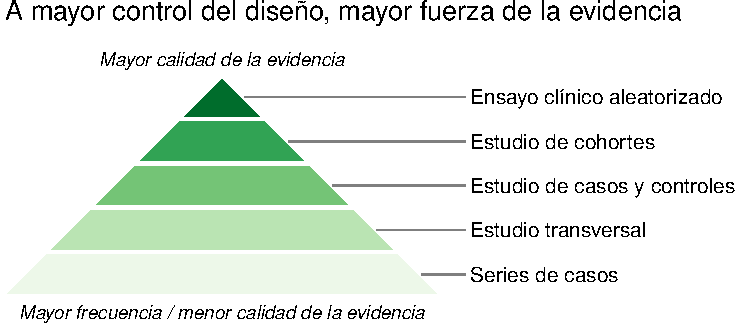
\includegraphics[keepaspectratio]{01-introduccion_files/figure-pdf/piramide-evidencia-1.pdf}}

}

\caption{Jerarquía habitual de la evidencia científica según el tipo de
estudio.}

\end{figure}%

Cada uno de los capítulos siguientes sigue la misma estructura:
definición y características del diseño, ventajas e inconvenientes,
medidas estadísticas propias del tipo de estudio, y un ejemplo completo
resuelto con R.

\part{Diseños de estudio}

\chapter{Estudios descriptivos}\label{estudios-descriptivos}

Como se vio en el
\hyperref[introducciuxf3n-a-los-tipos-de-estudios-estaduxedsticos]{capítulo
de introducción}, la finalidad de un estudio puede ser puramente
descriptiva o analítica. El estudio descriptivo es el diseño
observacional más elemental de todos: no compara grupos, no contrasta
hipótesis y no pretende establecer relaciones causales. Su único
objetivo es cuantificar y describir con precisión cómo se distribuye un
fenómeno (una enfermedad, un hábito, una característica cualquiera) en
una población o en un conjunto de individuos, sirviendo habitualmente
como primer paso de una investigación más amplia.

\section{Definición y
características}\label{definiciuxf3n-y-caracteruxedsticas}

\begin{definition}[Estudio
descriptivo]\protect\hypertarget{def-descriptivos-estudio-descriptivo}{}\label{def-descriptivos-estudio-descriptivo}

Un \emph{estudio descriptivo} es un estudio observacional cuyo único
objetivo es cuantificar la frecuencia, la distribución o las
características de un fenómeno en una población o en un grupo de
individuos, sin comparar grupos de exposición ni plantear hipótesis
sobre relaciones causa-efecto.

\end{definition}

En la práctica, los estudios descriptivos adoptan habitualmente alguna
de estas formas:

\begin{itemize}
\tightlist
\item
  \textbf{Reporte de caso} (\emph{case report}): descripción detallada
  de un único individuo con una característica, enfermedad o evolución
  clínica de interés, generalmente por su rareza o por presentar rasgos
  inesperados.
\item
  \textbf{Serie de casos} (\emph{case series}): descripción de un
  conjunto de individuos, todos ellos con una misma característica (por
  ejemplo, todos los pacientes diagnosticados de una enfermedad en un
  hospital durante un periodo determinado), sin comparación con ningún
  grupo que no la presente.
\item
  \textbf{Estudio descriptivo de frecuencia poblacional}: cuantificación
  de la presencia de un fenómeno en toda una población o en una muestra
  representativa de ella, mediante medidas como proporciones o tasas,
  habitualmente desagregadas por variables como el tiempo, el lugar o
  las características de las personas (la tríada clásica
  \emph{tiempo-lugar-persona} de la vigilancia epidemiológica).
\end{itemize}

Lo que caracteriza a los tres es la ausencia de un \textbf{grupo de
comparación}: no existen individuos ``no expuestos'' o ``sin la
característica'' frente a los que contrastar los resultados. Por ello,
un estudio descriptivo puede informar, por ejemplo, de que el 8~\% de
una muestra de pacientes ingresados presenta una determinada
complicación, pero \textbf{no puede} establecer si esa frecuencia es
alta o baja en comparación con otro grupo, ni identificar qué factores
la explican, ni mucho menos afirmar que exista una relación de
causalidad. Para eso son necesarios los diseños analíticos que se
desarrollan en los capítulos siguientes.

\section{Ventajas e inconvenientes}\label{ventajas-e-inconvenientes}

\textbf{Ventajas}

\begin{itemize}
\tightlist
\item
  Son rápidos, sencillos y económicos de llevar a cabo en comparación
  con cualquier diseño analítico o experimental.
\item
  No requieren un grupo de comparación ni una hipótesis previa, por lo
  que son ideales para explorar fenómenos sobre los que apenas existe
  información.
\item
  Son la herramienta natural para generar nuevas hipótesis que después
  se pondrán a prueba con diseños analíticos.
\item
  Constituyen la base de los sistemas de vigilancia epidemiológica, al
  permitir detectar cambios en la frecuencia de una enfermedad a lo
  largo del tiempo.
\item
  Son, con frecuencia, el único diseño posible cuando el fenómeno de
  estudio es muy poco frecuente (enfermedades raras) o cuando se trata
  de fenómenos nuevos de los que apenas hay casos documentados.
\end{itemize}

\textbf{Inconvenientes}

\begin{itemize}
\tightlist
\item
  No permiten establecer asociaciones entre variables, al carecer de
  grupo de comparación.
\item
  No permiten en ningún caso establecer relaciones de causalidad.
\item
  Los reportes y series de casos suelen basarse en muestras pequeñas y
  no representativas (a menudo pacientes de un único centro), lo que
  limita mucho la generalización de los resultados.
\item
  Son especialmente vulnerables al sesgo de selección, ya que los casos
  que llegan a describirse suelen ser los más llamativos o los que
  acuden a centros concretos.
\item
  No permiten controlar factores de confusión, al no compararse ningún
  grupo.
\end{itemize}

\section{Medidas propias de este
diseño}\label{medidas-propias-de-este-diseuxf1o}

Los estudios descriptivos se apoyan en tres medidas de frecuencia muy
sencillas, pero que conviene definir con precisión porque son los
ladrillos con los que se construyen prácticamente todas las medidas de
los diseños analíticos que se estudiarán en los capítulos siguientes
(riesgos, \emph{odds}, incidencias, etc.).

\subsection{Razón}\label{razuxf3n}

\begin{definition}[Razón]\protect\hypertarget{def-descriptivos-razon}{}\label{def-descriptivos-razon}

Una \emph{razón} (\emph{ratio}) es el cociente entre dos cantidades de
naturaleza distinta, no necesariamente relacionadas como parte y todo,
es decir, el numerador no está necesariamente incluido en el
denominador.

\[R = \frac{a}{b}\]

donde \(a\) y \(b\) son los tamaños de dos grupos o cantidades
diferentes.

\end{definition}

\begin{tcolorbox}[enhanced jigsaw, arc=.35mm, bottomrule=.15mm, bottomtitle=1mm, breakable, colback=white, colbacktitle=quarto-callout-important-color!10!white, colframe=quarto-callout-important-color-frame, coltitle=black, left=2mm, leftrule=.75mm, opacityback=0, opacitybacktitle=0.6, rightrule=.15mm, title=\textcolor{quarto-callout-important-color}{\faExclamation}\hspace{0.5em}{Importante}, titlerule=0mm, toprule=.15mm, toptitle=1mm]

Como \(a\) y \(b\) pueden ser cantidades de cualquier magnitud y no
existe una relación de inclusión entre ellas, se tiene que

\[R \geq 0,\]

sin que exista, en general, ninguna cota superior.

\end{tcolorbox}

\begin{tcolorbox}[enhanced jigsaw, arc=.35mm, bottomrule=.15mm, bottomtitle=1mm, breakable, colback=white, colbacktitle=quarto-callout-note-color!10!white, colframe=quarto-callout-note-color-frame, coltitle=black, left=2mm, leftrule=.75mm, opacityback=0, opacitybacktitle=0.6, rightrule=.15mm, title=\textcolor{quarto-callout-note-color}{\faInfo}\hspace{0.5em}{Interpretación}, titlerule=0mm, toprule=.15mm, toptitle=1mm]

\begin{itemize}
\tightlist
\item
  Una razón se interpreta como el número de veces que la cantidad del
  numerador contiene, o representa, a la cantidad del denominador.
\item
  Por ejemplo, la \emph{razón de masculinidad} de una población es el
  cociente entre el número de hombres y el número de mujeres. Una razón
  de masculinidad de 0.9 indica que hay 0.9 hombres por cada mujer.
\end{itemize}

\end{tcolorbox}

\subsection{Proporción}\label{proporciuxf3n}

\begin{definition}[Proporción]\protect\hypertarget{def-descriptivos-proporcion}{}\label{def-descriptivos-proporcion}

Una \emph{proporción} es el cociente entre el número de individuos que
presentan una determinada característica y el número total de individuos
del grupo, de modo que el numerador está incluido en el denominador.

\[P = \frac{a}{a+b} = \frac{a}{n}\]

donde \(a\) es el número de individuos con la característica de interés
y \(n=a+b\) es el tamaño total del grupo.

\end{definition}

\begin{tcolorbox}[enhanced jigsaw, arc=.35mm, bottomrule=.15mm, bottomtitle=1mm, breakable, colback=white, colbacktitle=quarto-callout-important-color!10!white, colframe=quarto-callout-important-color-frame, coltitle=black, left=2mm, leftrule=.75mm, opacityback=0, opacitybacktitle=0.6, rightrule=.15mm, title=\textcolor{quarto-callout-important-color}{\faExclamation}\hspace{0.5em}{Importante}, titlerule=0mm, toprule=.15mm, toptitle=1mm]

Al estar el numerador incluido en el denominador, toda proporción cumple

\[0 \leq P \leq 1,\]

y puede expresarse también como porcentaje multiplicándola por 100.

\end{tcolorbox}

\begin{tcolorbox}[enhanced jigsaw, arc=.35mm, bottomrule=.15mm, bottomtitle=1mm, breakable, colback=white, colbacktitle=quarto-callout-note-color!10!white, colframe=quarto-callout-note-color-frame, coltitle=black, left=2mm, leftrule=.75mm, opacityback=0, opacitybacktitle=0.6, rightrule=.15mm, title=\textcolor{quarto-callout-note-color}{\faInfo}\hspace{0.5em}{Interpretación}, titlerule=0mm, toprule=.15mm, toptitle=1mm]

\begin{itemize}
\tightlist
\item
  Si \(P=0\) ningún individuo del grupo presenta la característica.
\item
  Si \(P=1\) todos los individuos del grupo presentan la característica.
\item
  Cuanto más próxima esté \(P\) a 1, mayor es la frecuencia relativa de
  la característica en el grupo.
\end{itemize}

\end{tcolorbox}

\subsection{Tasa}\label{tasa}

\begin{definition}[Tasa]\protect\hypertarget{def-descriptivos-tasa}{}\label{def-descriptivos-tasa}

Una \emph{tasa} (\emph{rate}) es una proporción que incorpora
explícitamente el tiempo en su denominador, expresado habitualmente en
unidades de \textbf{persona-tiempo} (personas-año, personas-mes, etc.),
es decir, la suma de los periodos de tiempo que cada individuo permanece
en riesgo de que ocurra el fenómeno de interés.

\[T = \frac{\mbox{número de eventos nuevos}}{\mbox{personas-tiempo en riesgo}}\cdot k\]

donde \(k\) es una constante (10, 100, 1,000, 100,000\ldots) que se
elige para expresar la tasa con cifras manejables.

\end{definition}

\begin{tcolorbox}[enhanced jigsaw, arc=.35mm, bottomrule=.15mm, bottomtitle=1mm, breakable, colback=white, colbacktitle=quarto-callout-important-color!10!white, colframe=quarto-callout-important-color-frame, coltitle=black, left=2mm, leftrule=.75mm, opacityback=0, opacitybacktitle=0.6, rightrule=.15mm, title=\textcolor{quarto-callout-important-color}{\faExclamation}\hspace{0.5em}{Importante}, titlerule=0mm, toprule=.15mm, toptitle=1mm]

Como el numerador no está incluido en el denominador (que tiene unidades
de tiempo y no de individuos), una tasa

\[T \geq 0\]

no está acotada superiormente y, a diferencia de la proporción,
\textbf{no es adimensional}: sus unidades son ``eventos por
persona-tiempo''.

\end{tcolorbox}

\begin{tcolorbox}[enhanced jigsaw, arc=.35mm, bottomrule=.15mm, bottomtitle=1mm, breakable, colback=white, colbacktitle=quarto-callout-note-color!10!white, colframe=quarto-callout-note-color-frame, coltitle=black, left=2mm, leftrule=.75mm, opacityback=0, opacitybacktitle=0.6, rightrule=.15mm, title=\textcolor{quarto-callout-note-color}{\faInfo}\hspace{0.5em}{Interpretación}, titlerule=0mm, toprule=.15mm, toptitle=1mm]

\begin{itemize}
\tightlist
\item
  La tasa mide la \emph{velocidad} con la que ocurren nuevos eventos en
  una población, teniendo en cuenta el tiempo real que cada individuo ha
  estado expuesto al riesgo.
\item
  Dos poblaciones pueden tener el mismo número absoluto de eventos y,
  sin embargo, tasas muy distintas si el tiempo de seguimiento o el
  tamaño de la población en riesgo difieren.
\item
  La proporción es adecuada cuando todos los individuos se observan
  durante el mismo periodo de tiempo; cuando el tiempo de seguimiento
  varía de un individuo a otro (por incorporaciones tardías, pérdidas de
  seguimiento o fallecimientos por otras causas), la tasa es la medida
  correcta porque cada individuo aporta solo el tiempo que realmente
  estuvo en riesgo.
\end{itemize}

\end{tcolorbox}

\begin{example}[]\protect\hypertarget{exm-descriptivos-tasa-incidencia}{}\label{exm-descriptivos-tasa-incidencia}

Se sigue durante el año 2026 a 8 personas sanas para observar la
aparición de una determinada enfermedad. No todas permanecen en riesgo
el año completo: algunas la desarrollan antes de que termine el
seguimiento (y dejan de estar en riesgo) y otra abandona el estudio
antes de tiempo (pérdida de seguimiento).

\[
\begin{array}{lccc}
\hline
\mbox{Individuo} & \mbox{Meses en riesgo} & \mbox{¿Caso nuevo?} & \mbox{Motivo de fin de seguimiento}\\
\hline
\mbox{Individuo 1} & 12 & \mbox{No} & \mbox{Fin del estudio}\\
\mbox{Individuo 2} & 12 & \mbox{No} & \mbox{Fin del estudio}\\
\mbox{Individuo 3} & 5  & \mbox{Sí} & \mbox{Aparición de la enfermedad}\\
\mbox{Individuo 4} & 12 & \mbox{No} & \mbox{Fin del estudio}\\
\mbox{Individuo 5} & 8  & \mbox{Sí} & \mbox{Aparición de la enfermedad}\\
\mbox{Individuo 6} & 12 & \mbox{No} & \mbox{Fin del estudio}\\
\mbox{Individuo 7} & 3  & \mbox{No} & \mbox{Pérdida de seguimiento}\\
\mbox{Individuo 8} & 12 & \mbox{No} & \mbox{Fin del estudio}\\
\hline
\end{array}
\]

El total de meses-persona observados es \(12+12+5+12+8+12+3+12=76\)
meses-persona, lo que equivale a \(76/12=6.33\) personas-año. El número
de casos nuevos es 2 (individuos 3 y 5). La tasa de incidencia es, por
tanto,

\[
T = \frac{2}{6.33}\cdot 1\,000 = 315.9 \mbox{ casos por cada } 1\,000 \mbox{ personas-año}.
\]

Nótese que el individuo 7, aunque solo se observó durante 3 meses,
contribuye igualmente al denominador con esos 3 meses-persona, y que ni
él ni los individuos que desarrollan la enfermedad aportan tiempo en
riesgo más allá del momento en que dejan de estarlo. (Se trata de un
ejemplo con un tamaño muestral reducido con fines exclusivamente
ilustrativos; en la práctica las tasas se calculan sobre poblaciones de
miles o millones de personas-año).

\end{example}

\section{Realización con R}\label{realizaciuxf3n-con-r}

Supongamos que un servicio de urgencias hospitalario registra, durante
un mes, todos los casos atendidos de una determinada enfermedad
infecciosa, anotando la edad, el sexo y la gravedad del cuadro clínico.
Se trata de una serie de casos: no hay ningún grupo de comparación, solo
se describe la frecuencia con la que se presenta cada característica
dentro de la serie.

\begin{Shaded}
\begin{Highlighting}[]
\NormalTok{casos }\OtherTok{\textless{}{-}} \FunctionTok{tibble}\NormalTok{(}
  \AttributeTok{id =} \DecValTok{1}\SpecialCharTok{:}\DecValTok{28}\NormalTok{,}
  \AttributeTok{edad =} \FunctionTok{c}\NormalTok{(}\DecValTok{4}\NormalTok{, }\DecValTok{67}\NormalTok{, }\DecValTok{45}\NormalTok{, }\DecValTok{2}\NormalTok{, }\DecValTok{78}\NormalTok{, }\DecValTok{34}\NormalTok{, }\DecValTok{56}\NormalTok{, }\DecValTok{81}\NormalTok{, }\DecValTok{29}\NormalTok{, }\DecValTok{5}\NormalTok{,}
           \DecValTok{72}\NormalTok{, }\DecValTok{41}\NormalTok{, }\DecValTok{19}\NormalTok{, }\DecValTok{63}\NormalTok{, }\DecValTok{8}\NormalTok{, }\DecValTok{55}\NormalTok{, }\DecValTok{39}\NormalTok{, }\DecValTok{74}\NormalTok{, }\DecValTok{47}\NormalTok{, }\DecValTok{3}\NormalTok{,}
           \DecValTok{68}\NormalTok{, }\DecValTok{52}\NormalTok{, }\DecValTok{27}\NormalTok{, }\DecValTok{9}\NormalTok{, }\DecValTok{61}\NormalTok{, }\DecValTok{33}\NormalTok{, }\DecValTok{76}\NormalTok{, }\DecValTok{48}\NormalTok{),}
  \AttributeTok{sexo =} \FunctionTok{c}\NormalTok{(}\StringTok{"Mujer"}\NormalTok{, }\StringTok{"Hombre"}\NormalTok{, }\StringTok{"Mujer"}\NormalTok{, }\StringTok{"Mujer"}\NormalTok{, }\StringTok{"Hombre"}\NormalTok{, }\StringTok{"Hombre"}\NormalTok{, }\StringTok{"Mujer"}\NormalTok{, }\StringTok{"Mujer"}\NormalTok{,}
           \StringTok{"Hombre"}\NormalTok{, }\StringTok{"Mujer"}\NormalTok{, }\StringTok{"Hombre"}\NormalTok{, }\StringTok{"Mujer"}\NormalTok{, }\StringTok{"Hombre"}\NormalTok{, }\StringTok{"Mujer"}\NormalTok{, }\StringTok{"Hombre"}\NormalTok{, }\StringTok{"Hombre"}\NormalTok{,}
           \StringTok{"Mujer"}\NormalTok{, }\StringTok{"Mujer"}\NormalTok{, }\StringTok{"Hombre"}\NormalTok{, }\StringTok{"Mujer"}\NormalTok{, }\StringTok{"Mujer"}\NormalTok{, }\StringTok{"Hombre"}\NormalTok{, }\StringTok{"Mujer"}\NormalTok{, }\StringTok{"Hombre"}\NormalTok{,}
           \StringTok{"Hombre"}\NormalTok{, }\StringTok{"Mujer"}\NormalTok{, }\StringTok{"Mujer"}\NormalTok{, }\StringTok{"Hombre"}\NormalTok{),}
  \AttributeTok{gravedad =} \FunctionTok{c}\NormalTok{(}\StringTok{"Leve"}\NormalTok{, }\StringTok{"Grave"}\NormalTok{, }\StringTok{"Moderada"}\NormalTok{, }\StringTok{"Leve"}\NormalTok{, }\StringTok{"Grave"}\NormalTok{, }\StringTok{"Moderada"}\NormalTok{, }\StringTok{"Leve"}\NormalTok{, }\StringTok{"Grave"}\NormalTok{,}
               \StringTok{"Leve"}\NormalTok{, }\StringTok{"Leve"}\NormalTok{, }\StringTok{"Moderada"}\NormalTok{, }\StringTok{"Leve"}\NormalTok{, }\StringTok{"Leve"}\NormalTok{, }\StringTok{"Moderada"}\NormalTok{, }\StringTok{"Leve"}\NormalTok{, }\StringTok{"Moderada"}\NormalTok{,}
               \StringTok{"Leve"}\NormalTok{, }\StringTok{"Grave"}\NormalTok{, }\StringTok{"Moderada"}\NormalTok{, }\StringTok{"Leve"}\NormalTok{, }\StringTok{"Grave"}\NormalTok{, }\StringTok{"Leve"}\NormalTok{, }\StringTok{"Leve"}\NormalTok{, }\StringTok{"Leve"}\NormalTok{,}
               \StringTok{"Moderada"}\NormalTok{, }\StringTok{"Leve"}\NormalTok{, }\StringTok{"Grave"}\NormalTok{, }\StringTok{"Moderada"}\NormalTok{)}
\NormalTok{)}

\NormalTok{casos}
\end{Highlighting}
\end{Shaded}

\begin{verbatim}
# A tibble: 28 x 4
      id  edad sexo   gravedad
   <int> <dbl> <chr>  <chr>   
 1     1     4 Mujer  Leve    
 2     2    67 Hombre Grave   
 3     3    45 Mujer  Moderada
 4     4     2 Mujer  Leve    
 5     5    78 Hombre Grave   
 6     6    34 Hombre Moderada
 7     7    56 Mujer  Leve    
 8     8    81 Mujer  Grave   
 9     9    29 Hombre Leve    
10    10     5 Mujer  Leve    
# i 18 more rows
\end{verbatim}

Con \texttt{dplyr} es inmediato calcular la proporción de casos que
corresponde a cada categoría de gravedad, la primera medida descriptiva
de interés:

\begin{Shaded}
\begin{Highlighting}[]
\NormalTok{proporciones\_gravedad }\OtherTok{\textless{}{-}}\NormalTok{ casos }\SpecialCharTok{|\textgreater{}}
  \FunctionTok{count}\NormalTok{(gravedad) }\SpecialCharTok{|\textgreater{}}
  \FunctionTok{mutate}\NormalTok{(}\AttributeTok{proporcion =}\NormalTok{ n }\SpecialCharTok{/} \FunctionTok{sum}\NormalTok{(n),}
         \AttributeTok{porcentaje =} \FunctionTok{round}\NormalTok{(}\DecValTok{100} \SpecialCharTok{*}\NormalTok{ proporcion, }\DecValTok{1}\NormalTok{))}

\NormalTok{proporciones\_gravedad}
\end{Highlighting}
\end{Shaded}

\begin{verbatim}
# A tibble: 3 x 4
  gravedad     n proporcion porcentaje
  <chr>    <int>      <dbl>      <dbl>
1 Grave        6      0.214       21.4
2 Leve        14      0.5         50  
3 Moderada     8      0.286       28.6
\end{verbatim}

También puede describirse la razón entre sexos de la serie, y la
proporción de casos graves dentro de cada grupo de edad, agrupando
previamente la edad en tramos:

\begin{Shaded}
\begin{Highlighting}[]
\CommentTok{\# Razón hombres / mujeres en la serie de casos}
\NormalTok{razon\_sexo }\OtherTok{\textless{}{-}}\NormalTok{ casos }\SpecialCharTok{|\textgreater{}}
  \FunctionTok{count}\NormalTok{(sexo) }\SpecialCharTok{|\textgreater{}}
  \FunctionTok{pivot\_wider}\NormalTok{(}\AttributeTok{names\_from =}\NormalTok{ sexo, }\AttributeTok{values\_from =}\NormalTok{ n) }\SpecialCharTok{|\textgreater{}}
  \FunctionTok{mutate}\NormalTok{(}\AttributeTok{razon\_masculinidad =}\NormalTok{ Hombre }\SpecialCharTok{/}\NormalTok{ Mujer)}

\NormalTok{razon\_sexo}
\end{Highlighting}
\end{Shaded}

\begin{verbatim}
# A tibble: 1 x 3
  Hombre Mujer razon_masculinidad
   <int> <int>              <dbl>
1     13    15              0.867
\end{verbatim}

\begin{Shaded}
\begin{Highlighting}[]
\CommentTok{\# Proporción de casos graves por tramo de edad}
\NormalTok{casos\_edad }\OtherTok{\textless{}{-}}\NormalTok{ casos }\SpecialCharTok{|\textgreater{}}
  \FunctionTok{mutate}\NormalTok{(}\AttributeTok{tramo\_edad =} \FunctionTok{case\_when}\NormalTok{(}
\NormalTok{    edad }\SpecialCharTok{\textless{}} \DecValTok{15} \SpecialCharTok{\textasciitilde{}} \StringTok{"0{-}14 años"}\NormalTok{,}
\NormalTok{    edad }\SpecialCharTok{\textless{}} \DecValTok{65} \SpecialCharTok{\textasciitilde{}} \StringTok{"15{-}64 años"}\NormalTok{,}
    \ConstantTok{TRUE} \SpecialCharTok{\textasciitilde{}} \StringTok{"65 o más años"}
\NormalTok{  )) }\SpecialCharTok{|\textgreater{}}
  \FunctionTok{group\_by}\NormalTok{(tramo\_edad) }\SpecialCharTok{|\textgreater{}}
  \FunctionTok{summarise}\NormalTok{(}\AttributeTok{n =} \FunctionTok{n}\NormalTok{(),}
            \AttributeTok{graves =} \FunctionTok{sum}\NormalTok{(gravedad }\SpecialCharTok{==} \StringTok{"Grave"}\NormalTok{),}
            \AttributeTok{proporcion\_graves =} \FunctionTok{round}\NormalTok{(graves }\SpecialCharTok{/}\NormalTok{ n, }\DecValTok{2}\NormalTok{))}

\NormalTok{casos\_edad}
\end{Highlighting}
\end{Shaded}

\begin{verbatim}
# A tibble: 3 x 4
  tramo_edad        n graves proporcion_graves
  <chr>         <int>  <int>             <dbl>
1 0-14 años         6      0              0   
2 15-64 años       15      0              0   
3 65 o más años     7      6              0.86
\end{verbatim}

Si, además, se conociera cuántos días ha permanecido cada paciente
ingresado (por ejemplo, porque los casos graves requieren
hospitalización), podría calcularse una tasa de nuevos casos graves por
cada 1000 días-paciente de estancia, lo que ilustra cómo la misma lógica
de las tasas se aplica también dentro de un estudio descriptivo:

\begin{Shaded}
\begin{Highlighting}[]
\NormalTok{estancias }\OtherTok{\textless{}{-}}\NormalTok{ casos }\SpecialCharTok{|\textgreater{}}
  \FunctionTok{filter}\NormalTok{(gravedad }\SpecialCharTok{\%in\%} \FunctionTok{c}\NormalTok{(}\StringTok{"Moderada"}\NormalTok{, }\StringTok{"Grave"}\NormalTok{)) }\SpecialCharTok{|\textgreater{}}
  \FunctionTok{mutate}\NormalTok{(}\AttributeTok{dias\_estancia =} \FunctionTok{c}\NormalTok{(}\DecValTok{6}\NormalTok{, }\DecValTok{9}\NormalTok{, }\DecValTok{4}\NormalTok{, }\DecValTok{10}\NormalTok{, }\DecValTok{5}\NormalTok{, }\DecValTok{3}\NormalTok{, }\DecValTok{8}\NormalTok{, }\DecValTok{7}\NormalTok{, }\DecValTok{6}\NormalTok{, }\DecValTok{11}\NormalTok{, }\DecValTok{4}\NormalTok{, }\DecValTok{9}\NormalTok{, }\DecValTok{7}\NormalTok{, }\DecValTok{5}\NormalTok{))}

\NormalTok{tasa\_complicacion }\OtherTok{\textless{}{-}}\NormalTok{ estancias }\SpecialCharTok{|\textgreater{}}
  \FunctionTok{summarise}\NormalTok{(}
    \AttributeTok{dias\_persona =} \FunctionTok{sum}\NormalTok{(dias\_estancia),}
    \AttributeTok{casos\_graves =} \FunctionTok{sum}\NormalTok{(gravedad }\SpecialCharTok{==} \StringTok{"Grave"}\NormalTok{),}
    \AttributeTok{tasa\_x1000 =} \FunctionTok{round}\NormalTok{(}\DecValTok{1000} \SpecialCharTok{*}\NormalTok{ casos\_graves }\SpecialCharTok{/}\NormalTok{ dias\_persona, }\DecValTok{1}\NormalTok{)}
\NormalTok{  )}

\NormalTok{tasa\_complicacion}
\end{Highlighting}
\end{Shaded}

\begin{verbatim}
# A tibble: 1 x 3
  dias_persona casos_graves tasa_x1000
         <dbl>        <int>      <dbl>
1           94            6       63.8
\end{verbatim}

Por último, un diagrama de barras permite visualizar de un vistazo la
distribución de la gravedad de los casos, la representación gráfica más
habitual de una variable cualitativa en un estudio descriptivo:

\begin{Shaded}
\begin{Highlighting}[]
\FunctionTok{ggplot}\NormalTok{(proporciones\_gravedad, }\FunctionTok{aes}\NormalTok{(}\AttributeTok{x =} \FunctionTok{fct\_reorder}\NormalTok{(gravedad, proporcion, }\AttributeTok{.desc =} \ConstantTok{TRUE}\NormalTok{),}
                                   \AttributeTok{y =}\NormalTok{ proporcion)) }\SpecialCharTok{+}
  \FunctionTok{geom\_col}\NormalTok{(}\AttributeTok{fill =} \StringTok{"steelblue"}\NormalTok{) }\SpecialCharTok{+}
  \FunctionTok{geom\_text}\NormalTok{(}\FunctionTok{aes}\NormalTok{(}\AttributeTok{label =} \FunctionTok{paste0}\NormalTok{(porcentaje, }\StringTok{"\%"}\NormalTok{)), }\AttributeTok{vjust =} \SpecialCharTok{{-}}\FloatTok{0.5}\NormalTok{) }\SpecialCharTok{+}
  \FunctionTok{scale\_y\_continuous}\NormalTok{(}\AttributeTok{labels =}\NormalTok{ scales}\SpecialCharTok{::}\NormalTok{percent, }\AttributeTok{limits =} \FunctionTok{c}\NormalTok{(}\DecValTok{0}\NormalTok{, }\FunctionTok{max}\NormalTok{(proporciones\_gravedad}\SpecialCharTok{$}\NormalTok{proporcion) }\SpecialCharTok{*} \FloatTok{1.2}\NormalTok{)) }\SpecialCharTok{+}
  \FunctionTok{labs}\NormalTok{(}\AttributeTok{x =} \StringTok{"Gravedad del cuadro clínico"}\NormalTok{, }\AttributeTok{y =} \StringTok{"Proporción de casos"}\NormalTok{,}
       \AttributeTok{title =} \StringTok{"Gravedad de los casos atendidos en urgencias"}\NormalTok{) }\SpecialCharTok{+}
  \FunctionTok{theme\_minimal}\NormalTok{()}
\end{Highlighting}
\end{Shaded}

\begin{figure}[H]

{\centering \pandocbounded{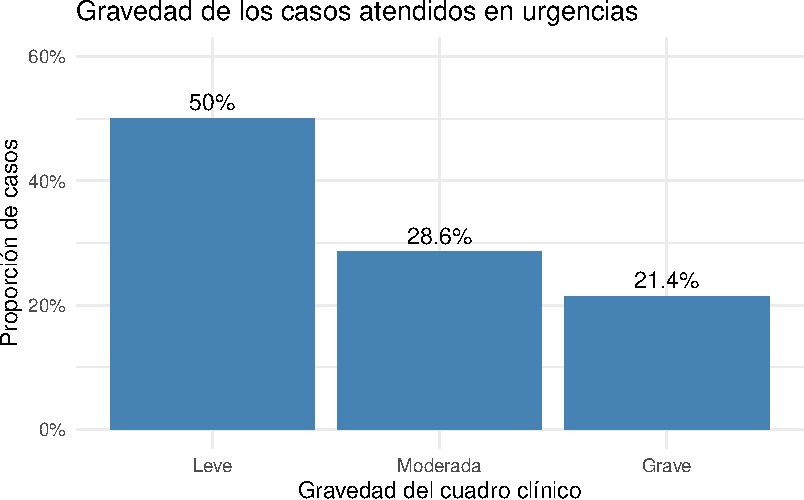
\includegraphics[keepaspectratio]{02-estudios-descriptivos_files/figure-pdf/grafico-proporciones-1.pdf}}

}

\caption{Distribución de la gravedad de los casos registrados en
urgencias durante el mes.}

\end{figure}%

Los resultados describen la serie de casos, pero no permiten ir más
allá: puede afirmarse que algo más de la mitad de los casos de esta
serie fueron leves y que la proporción de cuadros graves es mayor entre
los mayores de 65 años, pero no puede concluirse que la edad
\emph{cause} una mayor gravedad, porque no se dispone de ningún grupo de
comparación con el que contrastar esa diferencia ni se han controlado
otros factores que pudieran explicarla.

\section{Cuándo utilizar este
diseño}\label{cuuxe1ndo-utilizar-este-diseuxf1o}

Un estudio descriptivo es la elección adecuada cuando todavía se sabe
poco sobre un fenómeno y el objetivo prioritario es simplemente
cuantificarlo: en las primeras fases de un brote epidemiológico, en la
vigilancia rutinaria de enfermedades, al documentar un caso clínico
inusual, o al estudiar enfermedades tan raras que reunir un grupo de
comparación resulta inviable. Su gran ventaja es la sencillez y la
rapidez con la que aporta una primera fotografía del problema, que sirve
para generar hipótesis sobre posibles factores asociados. Sin embargo,
en cuanto la pregunta de investigación pasa de ``¿con qué frecuencia
ocurre esto?'' a ``¿por qué ocurre?'' o ``¿qué lo explica?'', un diseño
descriptivo deja de ser suficiente y es necesario recurrir a un diseño
analítico, como el \href{03-estudios-transversales.qmd}{estudio
transversal} o el \href{04-estudios-cohortes.qmd}{estudio de cohortes},
que sí incorporan un grupo de comparación frente al que contrastar los
resultados.

\chapter{Estudios transversales}\label{estudios-transversales}

Como se adelantó en el
\hyperref[introducciuxf3n-a-los-tipos-de-estudios-estaduxedsticos]{capítulo
de introducción}, un estudio transversal es un tipo de estudio
observacional en el que la exposición y el resultado se miden en un
único momento del tiempo sobre los mismos individuos. A diferencia de
los diseños longitudinales, que siguen a los sujetos a lo largo del
tiempo, el estudio transversal puede entenderse como una ``fotografía''
de la población: se toma una muestra en un instante concreto y se
registra simultáneamente el estado de todas las variables de interés.

\section{Definición y
características}\label{definiciuxf3n-y-caracteruxedsticas-1}

\begin{definition}[Estudio
transversal]\protect\hypertarget{def-transversales-estudio-transversal}{}\label{def-transversales-estudio-transversal}

Un \emph{estudio transversal} (también llamado \emph{estudio de
prevalencia} o, en inglés, \emph{cross-sectional study}) es un estudio
observacional en el que se selecciona una muestra de la población
general, sin tener en cuenta ni la exposición ni el resultado de los
individuos, y se miden todas las variables de interés en un único
momento del tiempo.

\end{definition}

La característica que define a este diseño es la forma de seleccionar la
muestra: los individuos se eligen de la población general (por ejemplo,
mediante un muestreo aleatorio), sin condicionar la selección al hecho
de estar expuestos o no, ni al hecho de presentar o no el resultado de
interés. Esto lo distingue tanto del
\href{04-estudios-cohortes.qmd}{estudio de cohortes}, que selecciona la
muestra según la exposición, como del
\href{05-estudios-casos-controles.qmd}{estudio de casos y controles},
que la selecciona según el resultado.

Un estudio transversal puede tener dos finalidades distintas, que a
menudo se combinan en la práctica:

\begin{itemize}
\tightlist
\item
  \textbf{Uso descriptivo}: estimar la prevalencia de una enfermedad,
  una opinión, un hábito o cualquier otro fenómeno en la población, sin
  comparar grupos. Este es el uso más habitual y el que da nombre
  alternativo al diseño (estudio de prevalencia).
\item
  \textbf{Uso analítico}: comparar la prevalencia del resultado entre
  distintos subgrupos definidos por una variable de exposición, con el
  fin de detectar posibles asociaciones. Sin embargo, como la exposición
  y el resultado se miden al mismo tiempo, no es posible establecer con
  certeza cuál precedió a cuál, por lo que las asociaciones observadas
  deben interpretarse con cautela.
\end{itemize}

\section{Ventajas e inconvenientes}\label{ventajas-e-inconvenientes-1}

\begin{itemize}
\tightlist
\item
  \textbf{Rapidez y bajo coste}: al no requerir seguimiento de los
  individuos, los estudios transversales suelen ejecutarse en mucho
  menos tiempo y con muchos menos recursos que los diseños
  longitudinales.
\item
  \textbf{Sencillez}: no es necesario localizar y mantener el contacto
  con los participantes durante un periodo prolongado, por lo que las
  pérdidas de seguimiento no son un problema.
\item
  \textbf{Utilidad para la planificación sanitaria}: al estimar la
  prevalencia de un problema de salud, son la herramienta natural para
  dimensionar recursos y priorizar políticas públicas.
\item
  \textbf{Imposibilidad de establecer causalidad}: al medirse la
  exposición y el resultado en el mismo momento, no se puede determinar
  la secuencia temporal entre ambas, lo que impide concluir que la
  exposición precede (y por tanto puede causar) al resultado.
\item
  \textbf{Sesgo de prevalencia-incidencia (o sesgo de Neyman)}: la
  muestra solo incluye a los individuos que en ese momento tienen la
  enfermedad, es decir, a los supervivientes o casos de duración
  suficiente para ser detectados en el corte transversal. Los casos que
  se curan rápidamente o que fallecen pronto tienden a quedar excluidos,
  sesgando las estimaciones.
\item
  \textbf{Poco adecuado para enfermedades raras o de corta duración}: si
  la prevalencia es muy baja o el episodio es muy breve, la probabilidad
  de capturar casos en un único corte temporal es pequeña, por lo que se
  necesitarían muestras enormes para obtener estimaciones precisas.
\end{itemize}

\section{Medidas propias de este
diseño}\label{medidas-propias-de-este-diseuxf1o-1}

\subsection{Prevalencia}\label{prevalencia}

La medida más característica del estudio transversal es la prevalencia,
que cuantifica qué proporción de la población presenta el resultado de
interés en el momento del corte.

\begin{definition}[Prevalencia]\protect\hypertarget{def-transversales-prevalencia}{}\label{def-transversales-prevalencia}

Dada una muestra de \(n\) individuos representativa de una población, de
los cuales \(a\) presentan el resultado de interés (casos) en el momento
del estudio, la \emph{prevalencia} (puntual) se define como

\[P = \frac{a}{n}\]

Habitualmente se expresa como porcentaje (multiplicando por 100) o como
número de casos por cada 1000, 10 000 o 100 000 habitantes, según la
frecuencia del fenómeno estudiado.

\end{definition}

\begin{tcolorbox}[enhanced jigsaw, arc=.35mm, bottomrule=.15mm, bottomtitle=1mm, breakable, colback=white, colbacktitle=quarto-callout-important-color!10!white, colframe=quarto-callout-important-color-frame, coltitle=black, left=2mm, leftrule=.75mm, opacityback=0, opacitybacktitle=0.6, rightrule=.15mm, title=\textcolor{quarto-callout-important-color}{\faExclamation}\hspace{0.5em}{Importante}, titlerule=0mm, toprule=.15mm, toptitle=1mm]

Como la prevalencia es una proporción, se cumple que

\[0 \leq P \leq 1,\]

siendo \(0\) cuando ningún individuo de la muestra presenta el resultado
y \(1\) (o el 100\%) cuando todos lo presentan.

\end{tcolorbox}

\begin{tcolorbox}[enhanced jigsaw, arc=.35mm, bottomrule=.15mm, bottomtitle=1mm, breakable, colback=white, colbacktitle=quarto-callout-note-color!10!white, colframe=quarto-callout-note-color-frame, coltitle=black, left=2mm, leftrule=.75mm, opacityback=0, opacitybacktitle=0.6, rightrule=.15mm, title=\textcolor{quarto-callout-note-color}{\faInfo}\hspace{0.5em}{Interpretación}, titlerule=0mm, toprule=.15mm, toptitle=1mm]

\begin{itemize}
\tightlist
\item
  Cuanto más próxima esté \(P\) a \(0\), menos extendido está el
  fenómeno en la población.
\item
  Cuanto más próxima esté \(P\) a \(1\), más extendido está el fenómeno
  en la población.
\item
  La prevalencia depende tanto de la frecuencia con la que aparecen los
  casos nuevos (incidencia) como de la duración media del episodio: una
  enfermedad crónica de larga duración puede tener una prevalencia alta
  aunque su incidencia sea baja.
\end{itemize}

\end{tcolorbox}

\begin{example}[]\protect\hypertarget{exm-transversales-prevalencia}{}\label{exm-transversales-prevalencia}

En un estudio transversal se seleccionó una muestra aleatoria de
\(n=500\) habitantes de una ciudad y se midió su presión arterial en una
única visita. De ellos, \(a=45\) presentaban hipertensión arterial en el
momento de la medición. La prevalencia puntual de hipertensión en esta
muestra es

\[P = \frac{a}{n} = \frac{45}{500} = 0.09.\]

Es decir, la prevalencia estimada de hipertensión en esta población es
del \(9\%\), o dicho de otra forma, de aproximadamente 90 casos por cada
1000 habitantes.

\end{example}

\subsection{Razón de prevalencias}\label{razuxf3n-de-prevalencias}

Cuando el estudio transversal se emplea con finalidad analítica,
comparando la prevalencia del resultado entre expuestos y no expuestos,
la medida de asociación habitual es la razón de prevalencias.

\begin{definition}[Razón de
prevalencias]\protect\hypertarget{def-transversales-razon-prevalencias}{}\label{def-transversales-razon-prevalencias}

Dada una tabla de contingencia que cruza una variable de exposición
binaria con un resultado binario,

\[
\begin{array}{lccc}
\hline
 & \mbox{Resultado} & \mbox{No resultado} & \mbox{Total}\\
\hline
\mbox{Expuestos} & a & b & a+b\\
\mbox{No expuestos} & c & d & c+d\\
\hline
\end{array}
\]

la \emph{razón de prevalencias} (\(RP\)) se define como el cociente
entre la prevalencia del resultado en el grupo de expuestos,
\(P_1 = \dfrac{a}{a+b}\), y la prevalencia del resultado en el grupo de
no expuestos, \(P_0 = \dfrac{c}{c+d}\),

\[RP = \frac{P_1}{P_0}.\]

\end{definition}

\begin{tcolorbox}[enhanced jigsaw, arc=.35mm, bottomrule=.15mm, bottomtitle=1mm, breakable, colback=white, colbacktitle=quarto-callout-important-color!10!white, colframe=quarto-callout-important-color-frame, coltitle=black, left=2mm, leftrule=.75mm, opacityback=0, opacitybacktitle=0.6, rightrule=.15mm, title=\textcolor{quarto-callout-important-color}{\faExclamation}\hspace{0.5em}{Importante}, titlerule=0mm, toprule=.15mm, toptitle=1mm]

La razón de prevalencias es siempre un número no negativo,

\[RP \geq 0,\]

sin límite superior.

\end{tcolorbox}

\begin{tcolorbox}[enhanced jigsaw, arc=.35mm, bottomrule=.15mm, bottomtitle=1mm, breakable, colback=white, colbacktitle=quarto-callout-note-color!10!white, colframe=quarto-callout-note-color-frame, coltitle=black, left=2mm, leftrule=.75mm, opacityback=0, opacitybacktitle=0.6, rightrule=.15mm, title=\textcolor{quarto-callout-note-color}{\faInfo}\hspace{0.5em}{Interpretación}, titlerule=0mm, toprule=.15mm, toptitle=1mm]

\begin{itemize}
\tightlist
\item
  Si \(RP=1\), la prevalencia del resultado es igual en expuestos y no
  expuestos, por lo que no hay asociación (en el corte estudiado) entre
  la exposición y el resultado.
\item
  Si \(RP>1\), la prevalencia del resultado es mayor entre los
  expuestos, lo que sugiere una asociación positiva entre exposición y
  resultado.
\item
  Si \(RP<1\), la prevalencia del resultado es menor entre los
  expuestos, lo que sugiere que la exposición podría ser un factor
  protector.
\item
  Al tratarse de un diseño transversal, esta asociación no permite
  concluir causalidad: no se puede descartar que sea el resultado el que
  influya sobre la exposición, o que ambos estén influidos por un tercer
  factor.
\end{itemize}

\end{tcolorbox}

\begin{example}[]\protect\hypertarget{exm-transversales-razon-prevalencias}{}\label{exm-transversales-razon-prevalencias}

En el mismo estudio transversal sobre 1000 personas, se registró además
si cada individuo era fumador. La tabla de contingencia entre el hábito
tabáquico y la presencia de bronquitis crónica en el momento de la
encuesta fue la siguiente:

\[
\begin{array}{lccc}
\hline
 & \mbox{Bronquitis} & \mbox{Sin bronquitis} & \mbox{Total}\\
\hline
\mbox{Fumadores} & 60 & 240 & 300\\
\mbox{No fumadores} & 35 & 665 & 700\\
\hline
\end{array}
\]

La prevalencia de bronquitis crónica en fumadores es
\(P_1 = \dfrac{60}{300} = 0.20\), y en no fumadores es
\(P_0 = \dfrac{35}{700} = 0.05\). La razón de prevalencias es por tanto

\[RP = \frac{P_1}{P_0} = \frac{0.20}{0.05} = 4.\]

Es decir, en el momento del corte, la prevalencia de bronquitis crónica
entre los fumadores es 4 veces la de los no fumadores.

\end{example}

\section{Realización con R}\label{realizaciuxf3n-con-r-1}

A continuación se simula un estudio transversal sobre \(n=180\)
individuos, en el que se mide una variable de exposición binaria
(exposición a un contaminante ambiental) y una variable de resultado
binaria (presencia de una afección respiratoria), ambas registradas en
el mismo momento del tiempo.

\begin{Shaded}
\begin{Highlighting}[]
\FunctionTok{set.seed}\NormalTok{(}\DecValTok{123}\NormalTok{)}
\NormalTok{n }\OtherTok{\textless{}{-}} \DecValTok{180}

\CommentTok{\# Exposición: el 40\% de la muestra está expuesta al contaminante}
\NormalTok{exposicion }\OtherTok{\textless{}{-}} \FunctionTok{rbinom}\NormalTok{(n, }\AttributeTok{size =} \DecValTok{1}\NormalTok{, }\AttributeTok{prob =} \FloatTok{0.4}\NormalTok{)}

\CommentTok{\# La probabilidad de presentar la afección depende de la exposición}
\NormalTok{p\_afeccion }\OtherTok{\textless{}{-}} \FunctionTok{ifelse}\NormalTok{(exposicion }\SpecialCharTok{==} \DecValTok{1}\NormalTok{, }\FloatTok{0.30}\NormalTok{, }\FloatTok{0.12}\NormalTok{)}
\NormalTok{resultado }\OtherTok{\textless{}{-}} \FunctionTok{rbinom}\NormalTok{(n, }\AttributeTok{size =} \DecValTok{1}\NormalTok{, }\AttributeTok{prob =}\NormalTok{ p\_afeccion)}

\NormalTok{datos }\OtherTok{\textless{}{-}} \FunctionTok{tibble}\NormalTok{(}
  \AttributeTok{id =} \DecValTok{1}\SpecialCharTok{:}\NormalTok{n,}
  \AttributeTok{exposicion =} \FunctionTok{factor}\NormalTok{(exposicion, }\AttributeTok{levels =} \FunctionTok{c}\NormalTok{(}\DecValTok{0}\NormalTok{, }\DecValTok{1}\NormalTok{), }\AttributeTok{labels =} \FunctionTok{c}\NormalTok{(}\StringTok{"No expuesto"}\NormalTok{, }\StringTok{"Expuesto"}\NormalTok{)),}
  \AttributeTok{resultado =} \FunctionTok{factor}\NormalTok{(resultado, }\AttributeTok{levels =} \FunctionTok{c}\NormalTok{(}\DecValTok{0}\NormalTok{, }\DecValTok{1}\NormalTok{), }\AttributeTok{labels =} \FunctionTok{c}\NormalTok{(}\StringTok{"Sin afección"}\NormalTok{, }\StringTok{"Con afección"}\NormalTok{))}
\NormalTok{)}

\NormalTok{datos}
\end{Highlighting}
\end{Shaded}

\begin{verbatim}
# A tibble: 180 x 3
      id exposicion  resultado   
   <int> <fct>       <fct>       
 1     1 No expuesto Sin afección
 2     2 Expuesto    Sin afección
 3     3 No expuesto Sin afección
 4     4 Expuesto    Sin afección
 5     5 Expuesto    Sin afección
 6     6 No expuesto Sin afección
 7     7 No expuesto Sin afección
 8     8 Expuesto    Sin afección
 9     9 No expuesto Con afección
10    10 No expuesto Con afección
# i 170 more rows
\end{verbatim}

En primer lugar se calcula la prevalencia global de la afección en toda
la muestra:

\begin{Shaded}
\begin{Highlighting}[]
\NormalTok{prevalencia\_global }\OtherTok{\textless{}{-}} \FunctionTok{mean}\NormalTok{(datos}\SpecialCharTok{$}\NormalTok{resultado }\SpecialCharTok{==} \StringTok{"Con afección"}\NormalTok{)}
\NormalTok{prevalencia\_global}
\end{Highlighting}
\end{Shaded}

\begin{verbatim}
[1] 0.1611111
\end{verbatim}

A continuación se calcula la prevalencia por grupo de exposición, junto
con el número de casos y el tamaño de cada grupo:

\begin{Shaded}
\begin{Highlighting}[]
\NormalTok{tabla\_prevalencias }\OtherTok{\textless{}{-}}\NormalTok{ datos }\SpecialCharTok{|\textgreater{}}
  \FunctionTok{group\_by}\NormalTok{(exposicion) }\SpecialCharTok{|\textgreater{}}
  \FunctionTok{summarise}\NormalTok{(}
    \AttributeTok{casos =} \FunctionTok{sum}\NormalTok{(resultado }\SpecialCharTok{==} \StringTok{"Con afección"}\NormalTok{),}
    \AttributeTok{n =} \FunctionTok{n}\NormalTok{(),}
    \AttributeTok{prevalencia =}\NormalTok{ casos }\SpecialCharTok{/}\NormalTok{ n}
\NormalTok{  )}

\NormalTok{tabla\_prevalencias}
\end{Highlighting}
\end{Shaded}

\begin{verbatim}
# A tibble: 2 x 4
  exposicion  casos     n prevalencia
  <fct>       <int> <int>       <dbl>
1 No expuesto    10   110      0.0909
2 Expuesto       19    70      0.271 
\end{verbatim}

Con estas dos prevalencias se obtiene la razón de prevalencias,
comparando el grupo expuesto con el grupo no expuesto:

\begin{Shaded}
\begin{Highlighting}[]
\NormalTok{rp }\OtherTok{\textless{}{-}}\NormalTok{ tabla\_prevalencias}\SpecialCharTok{$}\NormalTok{prevalencia[tabla\_prevalencias}\SpecialCharTok{$}\NormalTok{exposicion }\SpecialCharTok{==} \StringTok{"Expuesto"}\NormalTok{] }\SpecialCharTok{/}
\NormalTok{  tabla\_prevalencias}\SpecialCharTok{$}\NormalTok{prevalencia[tabla\_prevalencias}\SpecialCharTok{$}\NormalTok{exposicion }\SpecialCharTok{==} \StringTok{"No expuesto"}\NormalTok{]}

\NormalTok{rp}
\end{Highlighting}
\end{Shaded}

\begin{verbatim}
[1] 2.985714
\end{verbatim}

La prevalencia de la afección entre los expuestos al contaminante es, en
esta muestra, aproximadamente 3 veces la de los no expuestos, lo que
apunta a una posible asociación entre la exposición y el resultado (que,
tratándose de un diseño transversal, no puede interpretarse como
causal).

Por último, se calcula un intervalo de confianza al 95\% para la
prevalencia de cada grupo mediante \texttt{prop.test()}, y se
representan gráficamente las prevalencias con sus intervalos de
confianza:

\begin{Shaded}
\begin{Highlighting}[]
\NormalTok{intervalos }\OtherTok{\textless{}{-}}\NormalTok{ tabla\_prevalencias }\SpecialCharTok{|\textgreater{}}
  \FunctionTok{rowwise}\NormalTok{() }\SpecialCharTok{|\textgreater{}}
  \FunctionTok{mutate}\NormalTok{(}
    \AttributeTok{ic =} \FunctionTok{list}\NormalTok{(broom}\SpecialCharTok{::}\FunctionTok{tidy}\NormalTok{(}\FunctionTok{prop.test}\NormalTok{(casos, n)))}
\NormalTok{  ) }\SpecialCharTok{|\textgreater{}}
  \FunctionTok{unnest}\NormalTok{(ic) }\SpecialCharTok{|\textgreater{}}
  \FunctionTok{select}\NormalTok{(exposicion, casos, n, prevalencia, conf.low, conf.high)}

\NormalTok{intervalos}
\end{Highlighting}
\end{Shaded}

\begin{verbatim}
# A tibble: 2 x 6
  exposicion  casos     n prevalencia conf.low conf.high
  <fct>       <int> <int>       <dbl>    <dbl>     <dbl>
1 No expuesto    10   110      0.0909   0.0469     0.165
2 Expuesto       19    70      0.271    0.175      0.393
\end{verbatim}

\begin{Shaded}
\begin{Highlighting}[]
\FunctionTok{ggplot}\NormalTok{(intervalos, }\FunctionTok{aes}\NormalTok{(}\AttributeTok{x =}\NormalTok{ exposicion, }\AttributeTok{y =}\NormalTok{ prevalencia, }\AttributeTok{fill =}\NormalTok{ exposicion)) }\SpecialCharTok{+}
  \FunctionTok{geom\_col}\NormalTok{(}\AttributeTok{width =} \FloatTok{0.6}\NormalTok{) }\SpecialCharTok{+}
  \FunctionTok{geom\_errorbar}\NormalTok{(}\FunctionTok{aes}\NormalTok{(}\AttributeTok{ymin =}\NormalTok{ conf.low, }\AttributeTok{ymax =}\NormalTok{ conf.high), }\AttributeTok{width =} \FloatTok{0.15}\NormalTok{) }\SpecialCharTok{+}
  \FunctionTok{scale\_y\_continuous}\NormalTok{(}\AttributeTok{labels =}\NormalTok{ scales}\SpecialCharTok{::}\FunctionTok{percent\_format}\NormalTok{()) }\SpecialCharTok{+}
  \FunctionTok{scale\_fill\_brewer}\NormalTok{(}\AttributeTok{palette =} \StringTok{"Set2"}\NormalTok{) }\SpecialCharTok{+}
  \FunctionTok{labs}\NormalTok{(}
    \AttributeTok{x =} \StringTok{"Grupo de exposición"}\NormalTok{,}
    \AttributeTok{y =} \StringTok{"Prevalencia"}\NormalTok{,}
    \AttributeTok{title =} \StringTok{"Prevalencia de la afección respiratoria según exposición"}
\NormalTok{  ) }\SpecialCharTok{+}
  \FunctionTok{theme\_minimal}\NormalTok{() }\SpecialCharTok{+}
  \FunctionTok{theme}\NormalTok{(}\AttributeTok{legend.position =} \StringTok{"none"}\NormalTok{)}
\end{Highlighting}
\end{Shaded}

\begin{figure}[H]

{\centering \pandocbounded{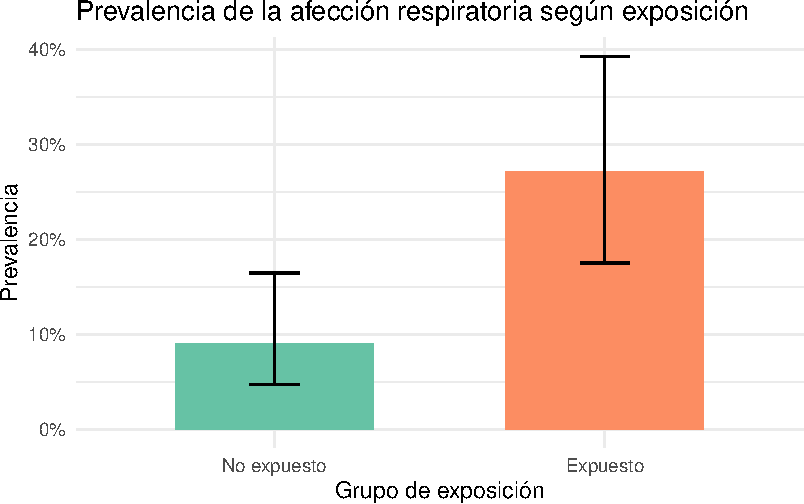
\includegraphics[keepaspectratio]{03-estudios-transversales_files/figure-pdf/grafico-prevalencias-1.pdf}}

}

\caption{Prevalencia de la afección respiratoria según la exposición al
contaminante, con intervalos de confianza al 95\%.}

\end{figure}%

El gráfico confirma que la prevalencia estimada en el grupo expuesto es
notablemente superior a la del grupo no expuesto, y que los intervalos
de confianza de ambos grupos no se solapan, lo que refuerza la idea de
que la diferencia observada difícilmente se debe solo al azar. No
obstante, al tratarse de un corte transversal, esta asociación debería
confirmarse con un diseño longitudinal, como un
\href{04-estudios-cohortes.qmd}{estudio de cohortes}, antes de extraer
conclusiones sobre causalidad.

\section{Cuándo utilizar este
diseño}\label{cuuxe1ndo-utilizar-este-diseuxf1o-1}

El estudio transversal es la herramienta de elección cuando el objetivo
principal es estimar la prevalencia de un fenómeno en un momento dado,
por ejemplo para planificar recursos sanitarios o describir el estado de
salud de una población. También resulta útil como paso previo,
exploratorio y económico, para generar hipótesis sobre posibles
asociaciones que después se pondrán a prueba con diseños más robustos.
Sin embargo, cuando el objetivo es establecer la secuencia temporal
entre una exposición y un resultado, o argumentar una posible relación
de causalidad, el estudio transversal no es el diseño adecuado: conviene
recurrir entonces a un \href{04-estudios-cohortes.qmd}{estudio de
cohortes}, que sigue a los individuos desde la exposición hacia el
resultado, o a un \href{05-estudios-casos-controles.qmd}{estudio de
casos y controles}, que parte del resultado para indagar
retrospectivamente en la exposición. La elección entre estas
alternativas dependerá de la frecuencia del resultado, del tiempo y los
recursos disponibles, y de si interesa priorizar la rapidez o la solidez
causal de las conclusiones.

\chapter{Estudios de cohortes}\label{estudios-de-cohortes}

Un \emph{estudio de cohortes} es un estudio observacional, analítico y
longitudinal en el que se parte de un grupo de individuos expuestos a un
determinado factor y de un grupo de individuos no expuestos a él, todos
ellos libres de la enfermedad o el resultado de interés en el momento
inicial, y se les sigue en el tiempo para comprobar quiénes desarrollan
dicho resultado. A diferencia del estudio transversal, en el que
exposición y resultado se observan en un único instante, en el estudio
de cohortes la secuencia temporal entre exposición y resultado queda
garantizada por diseño, lo que lo convierte en uno de los diseños
observacionales con mayor capacidad para sugerir relaciones causales.
Los conceptos generales de estudio observacional, analítico y
longitudinal se presentaron en el
\hyperref[introducciuxf3n-a-los-tipos-de-estudios-estaduxedsticos]{capítulo
de introducción}.

\section{Definición y
características}\label{definiciuxf3n-y-caracteruxedsticas-2}

\begin{definition}[Estudio de
cohortes]\protect\hypertarget{def-cohortes-estudio-cohortes}{}\label{def-cohortes-estudio-cohortes}

Un \emph{estudio de cohortes} es un estudio observacional en el que se
identifican dos o más grupos (cohortes) de individuos libres del
resultado de interés, definidos según su nivel de exposición a un factor
de estudio, y se les sigue durante un periodo de tiempo para comparar la
frecuencia con la que desarrollan dicho resultado.

\end{definition}

La característica esencial de este diseño es que la formación de los
grupos se realiza en función de la exposición, no del resultado: primero
se clasifica a los individuos en expuestos y no expuestos, y después se
observa la aparición de la enfermedad o evento de interés. Esto
contrasta con el estudio de casos y controles, en el que ocurre justo lo
contrario.

Según el momento en que se recogen los datos respecto al momento en que
se realiza el análisis, se distinguen dos variantes:

\begin{definition}[Cohorte
prospectiva]\protect\hypertarget{def-cohortes-cohorte-prospectiva}{}\label{def-cohortes-cohorte-prospectiva}

Una \emph{cohorte prospectiva} es aquella en la que la exposición se
determina en el momento presente y el seguimiento de los individuos se
realiza hacia adelante en el tiempo, recogiendo los datos del resultado
a medida que van ocurriendo.

\end{definition}

\begin{definition}[Cohorte retrospectiva o
histórica]\protect\hypertarget{def-cohortes-cohorte-retrospectiva}{}\label{def-cohortes-cohorte-retrospectiva}

Una \emph{cohorte retrospectiva} o \emph{histórica} es aquella en la que
tanto la exposición como el seguimiento y la aparición del resultado ya
han ocurrido en el pasado en el momento en que se inicia el estudio, de
modo que el investigador reconstruye la historia de exposición y
resultado a partir de registros u otras fuentes de información
existentes.

\end{definition}

\begin{tcolorbox}[enhanced jigsaw, arc=.35mm, bottomrule=.15mm, bottomtitle=1mm, breakable, colback=white, colbacktitle=quarto-callout-note-color!10!white, colframe=quarto-callout-note-color-frame, coltitle=black, left=2mm, leftrule=.75mm, opacityback=0, opacitybacktitle=0.6, rightrule=.15mm, title=\textcolor{quarto-callout-note-color}{\faInfo}\hspace{0.5em}{Interpretación}, titlerule=0mm, toprule=.15mm, toptitle=1mm]

La diferencia entre una cohorte prospectiva y una retrospectiva no está
en la lógica del diseño, que es idéntica en ambos casos (de la
exposición hacia el resultado), sino en el momento en que se sitúa el
investigador respecto al calendario de los hechos. En la cohorte
prospectiva el investigador espera a que ocurran los eventos; en la
retrospectiva, los eventos ya ocurrieron y se reconstruyen a partir de
historiales clínicos, registros administrativos u otras fuentes
documentales.

\end{tcolorbox}

\section{Ventajas e inconvenientes}\label{ventajas-e-inconvenientes-2}

El diseño de cohortes presenta una serie de ventajas frente a otros
estudios observacionales:

\begin{itemize}
\tightlist
\item
  Permite calcular directamente la incidencia de la enfermedad, tanto en
  expuestos como en no expuestos, ya que se parte de individuos libres
  de la enfermedad y se observa su aparición a lo largo del tiempo.
\item
  Es especialmente adecuado para el estudio de exposiciones poco
  frecuentes, ya que permite seleccionar deliberadamente un número
  suficiente de individuos expuestos.
\item
  Al hacer un seguimiento de los individuos, permite estudiar
  simultáneamente varios resultados o enfermedades asociados a una misma
  exposición.
\item
  Al respetar la secuencia temporal exposición-resultado, reduce algunos
  sesgos que afectan a los estudios transversales y facilita la
  interpretación causal.
\end{itemize}

Frente a estas ventajas, el diseño también presenta importantes
inconvenientes:

\begin{itemize}
\tightlist
\item
  Suele requerir un coste económico y una duración elevados, sobre todo
  en su variante prospectiva, ya que hay que esperar a que se acumulen
  suficientes casos.
\item
  Las pérdidas de seguimiento (individuos que abandonan el estudio antes
  de que finalice) pueden introducir sesgos si no son aleatorias
  respecto a la exposición o al resultado.
\item
  No resulta eficiente para el estudio de enfermedades raras, pues sería
  necesario seguir a un número muy elevado de individuos para observar
  un número suficiente de casos.
\end{itemize}

\section{Medidas propias de este
diseño}\label{medidas-propias-de-este-diseuxf1o-2}

El objetivo central de un estudio de cohortes es comparar la frecuencia
con la que aparece el resultado de interés en el grupo de expuestos
frente al grupo de no expuestos. Para ello se emplean tres medidas: la
incidencia acumulada, el riesgo relativo y el riesgo atribuible.

\subsection{Incidencia acumulada}\label{incidencia-acumulada}

\begin{definition}[Incidencia
acumulada]\protect\hypertarget{def-cohortes-incidencia-acumulada}{}\label{def-cohortes-incidencia-acumulada}

La \emph{incidencia acumulada} o \emph{riesgo} de un grupo es la
proporción de individuos que, estando libres de la enfermedad al inicio
del seguimiento, la desarrollan a lo largo de un periodo de tiempo fijo.
Si \(a\) es el número de casos nuevos que aparecen en un grupo de \(n\)
individuos seguidos durante dicho periodo, la incidencia acumulada se
define como

\[IA = \frac{a}{n}\]

\end{definition}

\begin{tcolorbox}[enhanced jigsaw, arc=.35mm, bottomrule=.15mm, bottomtitle=1mm, breakable, colback=white, colbacktitle=quarto-callout-important-color!10!white, colframe=quarto-callout-important-color-frame, coltitle=black, left=2mm, leftrule=.75mm, opacityback=0, opacitybacktitle=0.6, rightrule=.15mm, title=\textcolor{quarto-callout-important-color}{\faExclamation}\hspace{0.5em}{Importante}, titlerule=0mm, toprule=.15mm, toptitle=1mm]

Al ser una proporción, la incidencia acumulada cumple

\[0\leq IA \leq 1,\]

y suele expresarse también en tanto por ciento o por cada 1000, 10000,
etc. individuos, según la frecuencia del resultado.

\end{tcolorbox}

\subsection{Riesgo relativo}\label{riesgo-relativo}

\begin{definition}[Riesgo
relativo]\protect\hypertarget{def-cohortes-riesgo-relativo}{}\label{def-cohortes-riesgo-relativo}

El \emph{riesgo relativo} (RR) es el cociente entre la incidencia
acumulada en el grupo de expuestos (\(IA_E\)) y la incidencia acumulada
en el grupo de no expuestos (\(IA_{\bar E}\)):

\[RR = \frac{IA_E}{IA_{\bar E}}\]

\end{definition}

\begin{tcolorbox}[enhanced jigsaw, arc=.35mm, bottomrule=.15mm, bottomtitle=1mm, breakable, colback=white, colbacktitle=quarto-callout-important-color!10!white, colframe=quarto-callout-important-color-frame, coltitle=black, left=2mm, leftrule=.75mm, opacityback=0, opacitybacktitle=0.6, rightrule=.15mm, title=\textcolor{quarto-callout-important-color}{\faExclamation}\hspace{0.5em}{Importante}, titlerule=0mm, toprule=.15mm, toptitle=1mm]

El riesgo relativo es un cociente de dos proporciones, por lo que

\[RR \geq 0.\]

\end{tcolorbox}

\begin{tcolorbox}[enhanced jigsaw, arc=.35mm, bottomrule=.15mm, bottomtitle=1mm, breakable, colback=white, colbacktitle=quarto-callout-note-color!10!white, colframe=quarto-callout-note-color-frame, coltitle=black, left=2mm, leftrule=.75mm, opacityback=0, opacitybacktitle=0.6, rightrule=.15mm, title=\textcolor{quarto-callout-note-color}{\faInfo}\hspace{0.5em}{Interpretación}, titlerule=0mm, toprule=.15mm, toptitle=1mm]

\begin{itemize}
\tightlist
\item
  Si \(RR=1\), la incidencia es igual en expuestos y no expuestos, por
  lo que no existe asociación entre la exposición y el resultado.
\item
  Si \(RR>1\), la incidencia es mayor en expuestos, por lo que la
  exposición se comporta como un \emph{factor de riesgo}. Un \(RR=3\)
  indica que el riesgo de desarrollar el resultado es tres veces mayor
  en expuestos que en no expuestos.
\item
  Si \(RR<1\), la incidencia es menor en expuestos, por lo que la
  exposición se comporta como un \emph{factor protector}.
\end{itemize}

\end{tcolorbox}

\subsection{Riesgo atribuible}\label{riesgo-atribuible}

\begin{definition}[Riesgo
atribuible]\protect\hypertarget{def-cohortes-riesgo-atribuible}{}\label{def-cohortes-riesgo-atribuible}

El \emph{riesgo atribuible} (RA) es la diferencia entre la incidencia
acumulada en el grupo de expuestos y la incidencia acumulada en el grupo
de no expuestos:

\[RA = IA_E - IA_{\bar E}\]

El riesgo atribuible mide, en términos absolutos, el exceso de
incidencia del resultado que puede achacarse a la exposición. Cuando
además se calcula la proporción que ese exceso representa sobre la
incidencia total de los expuestos, se obtiene la \emph{fracción
atribuible en expuestos},

\[FAE = \frac{RA}{IA_E} = \frac{IA_E - IA_{\bar E}}{IA_E},\]

que indica qué proporción de los casos que ocurren entre los expuestos
se podrían evitar eliminando la exposición.

\end{definition}

\begin{tcolorbox}[enhanced jigsaw, arc=.35mm, bottomrule=.15mm, bottomtitle=1mm, breakable, colback=white, colbacktitle=quarto-callout-note-color!10!white, colframe=quarto-callout-note-color-frame, coltitle=black, left=2mm, leftrule=.75mm, opacityback=0, opacitybacktitle=0.6, rightrule=.15mm, title=\textcolor{quarto-callout-note-color}{\faInfo}\hspace{0.5em}{Interpretación}, titlerule=0mm, toprule=.15mm, toptitle=1mm]

Mientras que el riesgo relativo informa sobre la fuerza de la asociación
(en términos multiplicativos), el riesgo atribuible informa sobre el
impacto en salud pública de la exposición: dos exposiciones pueden tener
el mismo \(RR\) pero un \(RA\) muy distinto si las incidencias de base
son muy diferentes.

\end{tcolorbox}

\subsection{Ejemplo numérico}\label{ejemplo-numuxe9rico}

\begin{example}[]\protect\hypertarget{exm-cohortes-riesgo-relativo-atribuible}{}\label{exm-cohortes-riesgo-relativo-atribuible}

Se lleva a cabo un estudio de cohortes prospectivo para investigar la
relación entre el hábito de fumar y la aparición de bronquitis crónica.
Se reclutan 600 individuos libres de bronquitis crónica, de los cuales
200 son fumadores y 400 no fumadores, y se les sigue durante 10 años. Al
finalizar el seguimiento se obtiene la siguiente tabla de frecuencias:

\[
\begin{array}{lrrr}
\hline
 & \mbox{Bronquitis} & \mbox{No bronquitis} & \mbox{Total}\\
\hline
\mbox{Fumadores} & 40 & 160 & 200\\
\mbox{No fumadores} & 20 & 380 & 400\\
\hline
\end{array}
\]

\textbf{Incidencias acumuladas.} La incidencia acumulada en fumadores es

\[IA_E = \frac{40}{200} = 0.2 = 20\%,\]

y la incidencia acumulada en no fumadores es

\[IA_{\bar E} = \frac{20}{400} = 0.05 = 5\%.\]

\textbf{Riesgo relativo.}

\[RR = \frac{IA_E}{IA_{\bar E}} = \frac{0.2}{0.05} = 4.\]

El riesgo de desarrollar bronquitis crónica en los fumadores es 4 veces
el riesgo en los no fumadores, por lo que el tabaco se comporta como un
claro factor de riesgo.

\textbf{Riesgo atribuible.}

\[RA = IA_E - IA_{\bar E} = 0.2 - 0.05 = 0.15 = 15\%.\]

De cada 100 fumadores, 15 desarrollan bronquitis crónica como
consecuencia directa de fumar (los otros 5 de los 20 casos por 100 se
habrían producido igualmente por otras causas). La fracción atribuible
en expuestos es

\[FAE = \frac{RA}{IA_E} = \frac{0.15}{0.2} = 0.75 = 75\%,\]

es decir, el 75\% de los casos de bronquitis crónica que aparecen entre
los fumadores podrían evitarse si dejaran de fumar.

\end{example}

\section{Realización con R}\label{realizaciuxf3n-con-r-2}

\subsection{Cálculo de las medidas a partir de la tabla de
contingencia}\label{cuxe1lculo-de-las-medidas-a-partir-de-la-tabla-de-contingencia}

El primer paso es reproducir con R el cálculo manual del ejemplo
anterior, construyendo la tabla de contingencia como una matriz y
calculando a partir de ella las incidencias acumuladas, el riesgo
relativo y el riesgo atribuible.

\begin{Shaded}
\begin{Highlighting}[]
\CommentTok{\# Tabla de contingencia: filas = exposición, columnas = resultado (bronquitis, no bronquitis)}
\NormalTok{tabla }\OtherTok{\textless{}{-}} \FunctionTok{matrix}\NormalTok{(}\FunctionTok{c}\NormalTok{(}\DecValTok{40}\NormalTok{, }\DecValTok{160}\NormalTok{, }\DecValTok{20}\NormalTok{, }\DecValTok{380}\NormalTok{),}
                 \AttributeTok{nrow =} \DecValTok{2}\NormalTok{, }\AttributeTok{byrow =} \ConstantTok{TRUE}\NormalTok{,}
                 \AttributeTok{dimnames =} \FunctionTok{list}\NormalTok{(}\AttributeTok{Exposicion =} \FunctionTok{c}\NormalTok{(}\StringTok{"Fumadores"}\NormalTok{, }\StringTok{"No fumadores"}\NormalTok{),}
                                  \AttributeTok{Resultado =} \FunctionTok{c}\NormalTok{(}\StringTok{"Bronquitis"}\NormalTok{, }\StringTok{"No bronquitis"}\NormalTok{)))}
\NormalTok{tabla}
\end{Highlighting}
\end{Shaded}

\begin{verbatim}
              Resultado
Exposicion     Bronquitis No bronquitis
  Fumadores            40           160
  No fumadores         20           380
\end{verbatim}

\begin{Shaded}
\begin{Highlighting}[]
\CommentTok{\# Incidencias acumuladas}
\NormalTok{ia\_expuestos }\OtherTok{\textless{}{-}}\NormalTok{ tabla[}\StringTok{"Fumadores"}\NormalTok{, }\StringTok{"Bronquitis"}\NormalTok{] }\SpecialCharTok{/} \FunctionTok{sum}\NormalTok{(tabla[}\StringTok{"Fumadores"}\NormalTok{, ])}
\NormalTok{ia\_no\_expuestos }\OtherTok{\textless{}{-}}\NormalTok{ tabla[}\StringTok{"No fumadores"}\NormalTok{, }\StringTok{"Bronquitis"}\NormalTok{] }\SpecialCharTok{/} \FunctionTok{sum}\NormalTok{(tabla[}\StringTok{"No fumadores"}\NormalTok{, ])}
\FunctionTok{c}\NormalTok{(}\AttributeTok{IA\_expuestos =}\NormalTok{ ia\_expuestos, }\AttributeTok{IA\_no\_expuestos =}\NormalTok{ ia\_no\_expuestos)}
\end{Highlighting}
\end{Shaded}

\begin{verbatim}
   IA_expuestos IA_no_expuestos 
           0.20            0.05 
\end{verbatim}

\begin{Shaded}
\begin{Highlighting}[]
\CommentTok{\# Riesgo relativo}
\NormalTok{rr }\OtherTok{\textless{}{-}}\NormalTok{ ia\_expuestos }\SpecialCharTok{/}\NormalTok{ ia\_no\_expuestos}
\NormalTok{rr}
\end{Highlighting}
\end{Shaded}

\begin{verbatim}
[1] 4
\end{verbatim}

\begin{Shaded}
\begin{Highlighting}[]
\CommentTok{\# Riesgo atribuible y fracción atribuible en expuestos}
\NormalTok{ra }\OtherTok{\textless{}{-}}\NormalTok{ ia\_expuestos }\SpecialCharTok{{-}}\NormalTok{ ia\_no\_expuestos}
\NormalTok{fae }\OtherTok{\textless{}{-}}\NormalTok{ ra }\SpecialCharTok{/}\NormalTok{ ia\_expuestos}
\FunctionTok{c}\NormalTok{(}\AttributeTok{RA =}\NormalTok{ ra, }\AttributeTok{FAE =}\NormalTok{ fae)}
\end{Highlighting}
\end{Shaded}

\begin{verbatim}
  RA  FAE 
0.15 0.75 
\end{verbatim}

Los resultados, \(IA_E=0.2\), \(IA_{\bar E}=0.05\), \(RR=4\) y
\(RA=0.15\), coinciden exactamente con los obtenidos a mano.

\subsection{Análisis del tiempo hasta el evento con datos de
seguimiento}\label{anuxe1lisis-del-tiempo-hasta-el-evento-con-datos-de-seguimiento}

En muchos estudios de cohortes no todos los individuos completan el
mismo periodo de seguimiento: algunos abandonan el estudio antes de que
termine y otros lo finalizan sin haber desarrollado el resultado. En
ambos casos se dice que su tiempo de seguimiento está \emph{censurado}.
El análisis de supervivencia, implementado en el paquete
\texttt{survival}, permite tener en cuenta esta censura al comparar la
incidencia acumulada entre grupos.

En el siguiente ejemplo se simula una cohorte de 150 individuos, 75
expuestos y 75 no expuestos, con tiempos hasta el evento generados a
partir de una distribución exponencial (los expuestos tienen, en
promedio, un tiempo hasta el evento menor) y con un tiempo máximo de
seguimiento de 10 años que censura a los individuos que no han
presentado el evento antes de esa fecha.

\begin{Shaded}
\begin{Highlighting}[]
\FunctionTok{set.seed}\NormalTok{(}\DecValTok{123}\NormalTok{)}

\NormalTok{n\_grupo }\OtherTok{\textless{}{-}} \DecValTok{75}

\NormalTok{cohorte }\OtherTok{\textless{}{-}} \FunctionTok{tibble}\NormalTok{(}
  \AttributeTok{id =} \DecValTok{1}\SpecialCharTok{:}\NormalTok{(}\DecValTok{2} \SpecialCharTok{*}\NormalTok{ n\_grupo),}
  \AttributeTok{grupo =} \FunctionTok{rep}\NormalTok{(}\FunctionTok{c}\NormalTok{(}\StringTok{"Expuesto"}\NormalTok{, }\StringTok{"No expuesto"}\NormalTok{), }\AttributeTok{each =}\NormalTok{ n\_grupo),}
  \CommentTok{\# Tiempo hasta el evento: mayor tasa (menor tiempo medio) en expuestos}
  \AttributeTok{tiempo\_evento =} \FunctionTok{c}\NormalTok{(}\FunctionTok{rexp}\NormalTok{(n\_grupo, }\AttributeTok{rate =} \FloatTok{0.15}\NormalTok{),}
                     \FunctionTok{rexp}\NormalTok{(n\_grupo, }\AttributeTok{rate =} \FloatTok{0.06}\NormalTok{)),}
  \AttributeTok{tiempo\_max =} \DecValTok{10}\NormalTok{,}
  \AttributeTok{tiempo =} \FunctionTok{pmin}\NormalTok{(tiempo\_evento, tiempo\_max),}
  \AttributeTok{evento =} \FunctionTok{as.numeric}\NormalTok{(tiempo\_evento }\SpecialCharTok{\textless{}=}\NormalTok{ tiempo\_max)}
\NormalTok{)}

\NormalTok{cohorte }\SpecialCharTok{\%\textgreater{}\%}
  \FunctionTok{group\_by}\NormalTok{(grupo) }\SpecialCharTok{\%\textgreater{}\%}
  \FunctionTok{summarise}\NormalTok{(}\AttributeTok{n =} \FunctionTok{n}\NormalTok{(),}
            \AttributeTok{casos =} \FunctionTok{sum}\NormalTok{(evento),}
            \AttributeTok{incidencia\_acumulada =} \FunctionTok{mean}\NormalTok{(evento))}
\end{Highlighting}
\end{Shaded}

\begin{verbatim}
# A tibble: 2 x 4
  grupo           n casos incidencia_acumulada
  <chr>       <int> <dbl>                <dbl>
1 Expuesto       75    58                0.773
2 No expuesto    75    34                0.453
\end{verbatim}

Con los tiempos y el indicador de evento se construye un objeto de
superviviencia con \texttt{Surv()} y se ajusta una curva de Kaplan-Meier
por grupo con \texttt{survfit()}:

\begin{Shaded}
\begin{Highlighting}[]
\NormalTok{ajuste }\OtherTok{\textless{}{-}} \FunctionTok{survfit}\NormalTok{(}\FunctionTok{Surv}\NormalTok{(tiempo, evento) }\SpecialCharTok{\textasciitilde{}}\NormalTok{ grupo, }\AttributeTok{data =}\NormalTok{ cohorte)}
\FunctionTok{summary}\NormalTok{(ajuste)}\SpecialCharTok{$}\NormalTok{table}
\end{Highlighting}
\end{Shaded}

\begin{verbatim}
                  records n.max n.start events    rmean se(rmean)   median
grupo=Expuesto         75    75      75     58 5.631611 0.4008646 5.665241
grupo=No expuesto      75    75      75     34 7.518551 0.3681156       NA
                   0.95LCL  0.95UCL
grupo=Expuesto    3.924564 7.335592
grupo=No expuesto 7.613148       NA
\end{verbatim}

Para representar gráficamente las curvas se extraen los datos del ajuste
con \texttt{broom::tidy()}, que devuelve un data frame con la
probabilidad de supervivencia estimada en cada instante y grupo, y se
dibuja con \texttt{ggplot2}. La incidencia acumulada de cada grupo es el
complementario de la probabilidad de supervivencia (\(1 - S(t)\)):

\begin{Shaded}
\begin{Highlighting}[]
\NormalTok{ajuste\_df }\OtherTok{\textless{}{-}}\NormalTok{ broom}\SpecialCharTok{::}\FunctionTok{tidy}\NormalTok{(ajuste) }\SpecialCharTok{\%\textgreater{}\%}
  \FunctionTok{mutate}\NormalTok{(}\AttributeTok{grupo =} \FunctionTok{str\_remove}\NormalTok{(strata, }\StringTok{"grupo="}\NormalTok{),}
         \AttributeTok{incidencia\_acumulada =} \DecValTok{1} \SpecialCharTok{{-}}\NormalTok{ estimate)}

\FunctionTok{ggplot}\NormalTok{(ajuste\_df, }\FunctionTok{aes}\NormalTok{(}\AttributeTok{x =}\NormalTok{ time, }\AttributeTok{y =}\NormalTok{ incidencia\_acumulada, }\AttributeTok{color =}\NormalTok{ grupo)) }\SpecialCharTok{+}
  \FunctionTok{geom\_step}\NormalTok{(}\AttributeTok{linewidth =} \DecValTok{1}\NormalTok{) }\SpecialCharTok{+}
  \FunctionTok{labs}\NormalTok{(}\AttributeTok{x =} \StringTok{"Tiempo de seguimiento (años)"}\NormalTok{,}
       \AttributeTok{y =} \StringTok{"Incidencia acumulada estimada"}\NormalTok{,}
       \AttributeTok{color =} \StringTok{"Grupo"}\NormalTok{,}
       \AttributeTok{title =} \StringTok{"Incidencia acumulada de bronquitis crónica según exposición"}\NormalTok{) }\SpecialCharTok{+}
  \FunctionTok{scale\_y\_continuous}\NormalTok{(}\AttributeTok{labels =}\NormalTok{ scales}\SpecialCharTok{::}\NormalTok{percent) }\SpecialCharTok{+}
  \FunctionTok{theme\_minimal}\NormalTok{()}
\end{Highlighting}
\end{Shaded}

\pandocbounded{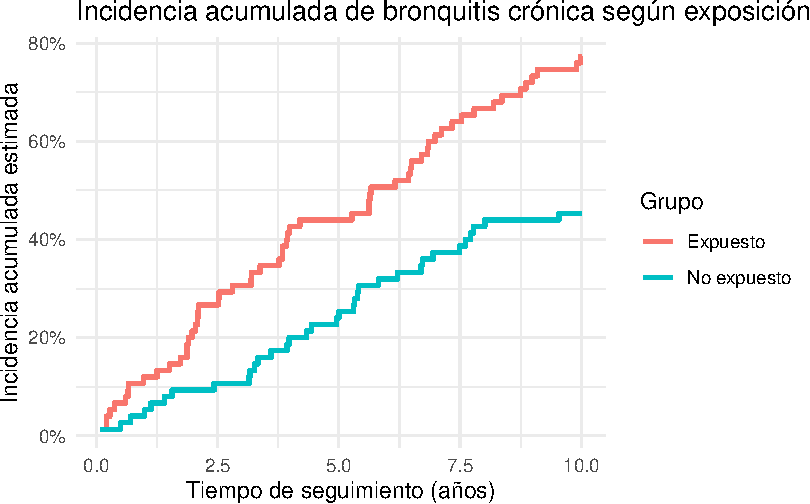
\includegraphics[keepaspectratio]{04-estudios-cohortes_files/figure-pdf/unnamed-chunk-7-1.pdf}}

Las curvas muestran cómo la incidencia acumulada crece más deprisa y
alcanza un nivel más alto en el grupo de expuestos que en el de no
expuestos a lo largo de todo el periodo de seguimiento, lo que es
coherente con un factor de riesgo. A diferencia del cálculo directo de
incidencias con una tabla de contingencia, este enfoque aprovecha toda
la información disponible de cada individuo, incluida la de quienes son
censurados antes de que finalice el seguimiento, en lugar de
descartarlos o tratarlos como si no hubieran desarrollado el resultado.

\section{Cuándo utilizar este
diseño}\label{cuuxe1ndo-utilizar-este-diseuxf1o-2}

El estudio de cohortes es la opción preferible cuando se dispone de
tiempo y recursos suficientes, la exposición de interés es poco
frecuente, o se quiere estudiar el efecto de una exposición sobre varios
resultados a la vez, ya que permite calcular directamente incidencias,
riesgos relativos y riesgos atribuibles. Cuando el resultado de interés
es una enfermedad rara, con periodos de latencia muy largos o cuando se
necesita una respuesta rápida y con un coste reducido, resulta más
eficiente recurrir a un \href{05-estudios-casos-controles.qmd}{estudio
de casos y controles}, que parte del resultado en lugar de la
exposición. Y cuando ni siquiera se necesita establecer una secuencia
temporal entre exposición y resultado, sino simplemente describir su
asociación en un momento dado, puede bastar con un
\hyperref[estudios-transversales]{estudio transversal}, mucho más rápido
y barato de ejecutar aunque no permita calcular incidencias ni
establecer con claridad la dirección de la relación.

\chapter{Estudios de casos y
controles}\label{estudios-de-casos-y-controles}

El estudio de casos y controles es un diseño observacional y analítico
que, a diferencia del \hyperref[estudios-de-cohortes]{estudio de
cohortes}, recorre el tiempo en sentido inverso: en lugar de partir de
la exposición y esperar a que aparezca el resultado, se parte del
resultado, ya ocurrido, y se indaga hacia atrás en busca de la
exposición pasada. Por este motivo se trata, casi siempre, de un diseño
retrospectivo (véase el
\hyperref[introducciuxf3n-a-los-tipos-de-estudios-estaduxedsticos]{capítulo
de introducción} para la distinción entre los criterios de clasificación
de los estudios). Se seleccionan dos grupos de individuos definidos por
su estado respecto al resultado (los \emph{casos}, que presentan la
enfermedad o el evento de interés, y los \emph{controles}, que no lo
presentan) y se compara la frecuencia con la que unos y otros estuvieron
expuestos en el pasado al factor de estudio.

\section{Definición y
características}\label{definiciuxf3n-y-caracteruxedsticas-3}

\begin{definition}[Estudio de casos y
controles]\protect\hypertarget{def-casoscontroles-estudio-casos-controles}{}\label{def-casoscontroles-estudio-casos-controles}

Un \emph{estudio de casos y controles} es un estudio observacional,
analítico y habitualmente retrospectivo en el que se seleccionan dos
grupos de individuos según la presencia (\emph{casos}) o ausencia
(\emph{controles}) del resultado de interés, y se compara
retrospectivamente la proporción de expuestos al factor de estudio en
cada uno de los dos grupos.

\end{definition}

El diseño se articula en torno a dos decisiones críticas, de las que
depende en buena medida la validez del estudio:

\begin{itemize}
\tightlist
\item
  \textbf{Selección de los casos.} Deben definirse con criterios
  diagnósticos claros y explícitos, de forma que no haya ambigüedad
  sobre quién es o no un caso. Es preferible utilizar casos
  \emph{incidentes} (de nueva aparición) frente a casos
  \emph{prevalentes} (ya existentes en el momento del estudio), porque
  estos últimos pueden reflejar factores asociados a la supervivencia
  con la enfermedad más que a su aparición.
\item
  \textbf{Selección de los controles.} Deben proceder de la misma
  población de la que surgen los casos (la llamada \emph{población base}
  o \emph{population at risk}), de modo que, si hubieran desarrollado la
  enfermedad, habrían sido incluidos como casos. Un control mal elegido
  ---que no sea representativo de esa población base--- es la fuente de
  sesgo más frecuente y más difícil de corregir en este tipo de
  estudios.
\end{itemize}

Una consecuencia importante de este diseño es que \textbf{no permite
calcular directamente ni la incidencia ni la prevalencia} de la
enfermedad. El motivo es que el número de casos y de controles no surge
de muestrear aleatoriamente la población y observar cuántos enferman,
sino que lo fija de antemano el propio investigador (por ejemplo, todos
los casos disponibles en un hospital durante un periodo, junto con el
doble de controles). Al no respetarse la proporción real de enfermos y
sanos en la población, cualquier medida que dependa de esa proporción
---como el riesgo relativo o la incidencia acumulada--- queda
distorsionada. Como se verá más adelante, esta limitación es
precisamente la que obliga a recurrir a la \emph{odds ratio} como medida
de asociación propia de este diseño.

\section{Ventajas e inconvenientes}\label{ventajas-e-inconvenientes-3}

\textbf{Ventajas:}

\begin{itemize}
\tightlist
\item
  Son estudios rápidos y baratos de realizar, ya que no requieren
  seguimiento de los individuos en el tiempo.
\item
  Son especialmente adecuados para el estudio de enfermedades raras,
  porque parten de un número fijo de casos ya identificados en lugar de
  esperar a que aparezcan en una cohorte.
\item
  Resultan también apropiados cuando el periodo de latencia entre la
  exposición y la enfermedad es muy largo, ya que evitan años de
  seguimiento.
\item
  Permiten estudiar simultáneamente varias exposiciones o factores de
  riesgo distintos para un mismo resultado.
\end{itemize}

\textbf{Inconvenientes:}

\begin{itemize}
\tightlist
\item
  Son susceptibles al \textbf{sesgo de memoria} (\emph{recall bias}):
  los casos, al haber sufrido la enfermedad, tienden a recordar y
  declarar con más detalle exposiciones pasadas que los controles.
\item
  Son susceptibles al \textbf{sesgo de selección de controles}, si estos
  no son verdaderamente representativos de la población base de la que
  proceden los casos.
\item
  No permiten calcular directamente la incidencia ni la prevalencia de
  la enfermedad, como se ha explicado.
\item
  La secuencia temporal entre exposición y resultado, al reconstruirse
  retrospectivamente, puede ser difícil de establecer con certeza en
  algunos casos.
\end{itemize}

\section{Medidas propias de este
diseño}\label{medidas-propias-de-este-diseuxf1o-3}

Como la incidencia no puede calcularse en este diseño, no es posible
obtener el riesgo relativo tal y como se define en un
\hyperref[estudios-de-cohortes]{estudio de cohortes}. La medida de
asociación propia de los estudios de casos y controles es la \emph{razón
de momios} u \emph{Odds Ratio} (OR), que compara la \emph{odds} (el
momio) de haber estado expuesto entre los casos con la de haber estado
expuesto entre los controles.

Partiendo de una tabla de contingencia \(2\times 2\) que cruza la
exposición con la condición de caso o control,

\[
\begin{array}{lrrr}
\hline
 & \mbox{Casos} & \mbox{Controles} & \mbox{Total}\\
\hline
\mbox{Expuestos} & a & b & a+b\\
\mbox{No expuestos} & c & d & c+d\\
\hline
\mbox{Total} & a+c & b+d & n\\
\hline
\end{array}
\]

\begin{definition}[Odds
ratio]\protect\hypertarget{def-casoscontroles-odds-ratio}{}\label{def-casoscontroles-odds-ratio}

La \emph{odds} (o momio) de exposición entre los casos es el cociente
entre el número de casos expuestos y el número de casos no expuestos,

\[\mbox{Odds}_{\mbox{casos}} = \frac{a}{c},\]

y la odds de exposición entre los controles es el cociente entre el
número de controles expuestos y el número de controles no expuestos,

\[\mbox{Odds}_{\mbox{controles}} = \frac{b}{d}.\]

La \emph{Odds Ratio} (OR) se define como el cociente entre ambas odds,

\[OR = \frac{\mbox{Odds}_{\mbox{casos}}}{\mbox{Odds}_{\mbox{controles}}} = \frac{a/c}{b/d} = \frac{a\cdot d}{b\cdot c}.\]

\end{definition}

\begin{tcolorbox}[enhanced jigsaw, arc=.35mm, bottomrule=.15mm, bottomtitle=1mm, breakable, colback=white, colbacktitle=quarto-callout-important-color!10!white, colframe=quarto-callout-important-color-frame, coltitle=black, left=2mm, leftrule=.75mm, opacityback=0, opacitybacktitle=0.6, rightrule=.15mm, title=\textcolor{quarto-callout-important-color}{\faExclamation}\hspace{0.5em}{Importante}, titlerule=0mm, toprule=.15mm, toptitle=1mm]

Al ser un cociente de dos cantidades positivas, la odds ratio verifica

\[OR > 0,\]

y \(OR=1\) indica ausencia de asociación entre la exposición y el
resultado, ya que en ese caso la odds de exposición es idéntica en casos
y en controles.

\end{tcolorbox}

\begin{tcolorbox}[enhanced jigsaw, arc=.35mm, bottomrule=.15mm, bottomtitle=1mm, breakable, colback=white, colbacktitle=quarto-callout-note-color!10!white, colframe=quarto-callout-note-color-frame, coltitle=black, left=2mm, leftrule=.75mm, opacityback=0, opacitybacktitle=0.6, rightrule=.15mm, title=\textcolor{quarto-callout-note-color}{\faInfo}\hspace{0.5em}{Interpretación}, titlerule=0mm, toprule=.15mm, toptitle=1mm]

\begin{itemize}
\tightlist
\item
  Si \(OR=1\), la exposición no está asociada con la enfermedad.
\item
  Si \(OR>1\), la exposición está asociada positivamente con la
  enfermedad: los expuestos tienen una odds mayor de ser casos, por lo
  que la exposición se comporta como un \textbf{factor de riesgo}.
\item
  Si \(OR<1\), la exposición está asociada negativamente con la
  enfermedad: los expuestos tienen una odds menor de ser casos, por lo
  que la exposición se comporta como un \textbf{factor protector}.
\end{itemize}

\end{tcolorbox}

\begin{tcolorbox}[enhanced jigsaw, arc=.35mm, bottomrule=.15mm, bottomtitle=1mm, breakable, colback=white, colbacktitle=quarto-callout-note-color!10!white, colframe=quarto-callout-note-color-frame, coltitle=black, left=2mm, leftrule=.75mm, opacityback=0, opacitybacktitle=0.6, rightrule=.15mm, title=\textcolor{quarto-callout-note-color}{\faInfo}\hspace{0.5em}{Relación con el riesgo relativo}, titlerule=0mm, toprule=.15mm, toptitle=1mm]

En un \hyperref[estudios-de-cohortes]{estudio de cohortes} la medida
natural de asociación es el riesgo relativo (RR), que compara
directamente las incidencias (probabilidades) de enfermar entre
expuestos y no expuestos. En un estudio de casos y controles no es
posible calcular incidencias, por lo que el RR no puede obtenerse
directamente. Sin embargo, cuando la enfermedad estudiada es
\textbf{poco frecuente} en la población (el llamado \emph{supuesto de
enfermedad rara}, por ejemplo con una prevalencia inferior al 10\%), la
probabilidad de enfermar es muy pequeña tanto en expuestos como en no
expuestos, de modo que la odds de enfermar (probabilidad entre 1 menos
probabilidad) se aproxima mucho a la propia probabilidad. En estas
condiciones puede demostrarse que la odds ratio calculada en el estudio
de casos y controles constituye una buena aproximación del riesgo
relativo poblacional, \(OR \approx RR\), lo que permite interpretarla de
forma similar aunque los diseños sean muy distintos.

\end{tcolorbox}

La incertidumbre muestral de la OR se cuantifica mediante su intervalo
de confianza. Como la distribución de la OR es muy asimétrica, el
intervalo se construye habitualmente sobre su logaritmo, que se aproxima
mejor a una distribución normal.

\begin{definition}[Intervalo de confianza de la odds ratio (método de
Woolf)]\protect\hypertarget{def-casoscontroles-ic-odds-ratio}{}\label{def-casoscontroles-ic-odds-ratio}

El error estándar del logaritmo de la odds ratio se estima como

\[SE(\ln OR) = \sqrt{\frac{1}{a}+\frac{1}{b}+\frac{1}{c}+\frac{1}{d}},\]

y el intervalo de confianza al \((1-\alpha)\cdot 100\%\) para la OR,
conocido como método de Woolf, se obtiene deshaciendo el logaritmo tras
construir el intervalo en escala logarítmica,

\[IC_{(1-\alpha)\cdot100\%} = \exp\left(\ln(OR) \pm z_{1-\alpha/2}\sqrt{\frac{1}{a}+\frac{1}{b}+\frac{1}{c}+\frac{1}{d}}\right).\]

Para un nivel de confianza del 95\%, \(z_{0.975}=1.96\).

\end{definition}

\begin{example}[]\protect\hypertarget{exm-casoscontroles-odds-ratio}{}\label{exm-casoscontroles-odds-ratio}

Se quiere estudiar la asociación entre el consumo habitual de tabaco y
la aparición de cáncer de pulmón mediante un estudio de casos y
controles. Se seleccionan 100 casos (pacientes recién diagnosticados de
cáncer de pulmón) y 200 controles (pacientes sin cáncer de pulmón,
similares en edad y sexo), y se les pregunta retrospectivamente si han
sido fumadores habituales. Los resultados se resumen en la siguiente
tabla:

\[
\begin{array}{lrrr}
\hline
 & \mbox{Casos} & \mbox{Controles} & \mbox{Total}\\
\hline
\mbox{Fumadores} & 70 & 80 & 150\\
\mbox{No fumadores} & 30 & 120 & 150\\
\hline
\mbox{Total} & 100 & 200 & 300\\
\hline
\end{array}
\]

Con \(a=70\), \(b=80\), \(c=30\) y \(d=120\), la odds ratio es

\[OR = \frac{a\cdot d}{b\cdot c} = \frac{70\cdot 120}{80\cdot 30} = \frac{8400}{2400} = 3.5.\]

Es decir, la odds de haber fumado es 3.5 veces mayor entre los casos
(pacientes con cáncer de pulmón) que entre los controles, lo que sugiere
que el tabaco se comporta como un factor de riesgo para esta enfermedad.
Como se trata de una enfermedad poco frecuente en la población general,
esta OR puede interpretarse aproximadamente como el riesgo relativo.

Para calcular el intervalo de confianza al 95\%, se obtiene primero el
error estándar del logaritmo de la OR,

\[SE(\ln OR) = \sqrt{\frac{1}{70}+\frac{1}{80}+\frac{1}{30}+\frac{1}{120}} = \sqrt{0.0143+0.0125+0.0333+0.0083} = \sqrt{0.0684} = 0.2615,\]

y como \(\ln(3.5) = 1.2528\), el intervalo en escala logarítmica es

\[1.2528 \pm 1.96\cdot 0.2615 = 1.2528 \pm 0.5125 = (0.7403,\ 1.7653),\]

que, deshaciendo el logaritmo, da el intervalo de confianza para la OR

\[IC_{95\%} = (e^{0.7403},\ e^{1.7653}) = (2.10,\ 5.84).\]

Como el intervalo no contiene el valor 1, la asociación entre tabaco y
cáncer de pulmón es estadísticamente significativa al 95\% de confianza.

\end{example}

\section{Realización con R}\label{realizaciuxf3n-con-r-3}

El siguiente código reproduce en R el ejemplo anterior, calculando la OR
y su intervalo de confianza al 95\% a partir de la tabla \(2\times 2\)
para comprobar que coincide con el cálculo manual.

\begin{Shaded}
\begin{Highlighting}[]
\CommentTok{\# Tabla 2x2: filas = expuestos/no expuestos, columnas = casos/controles}
\NormalTok{tabla }\OtherTok{\textless{}{-}} \FunctionTok{matrix}\NormalTok{(}\FunctionTok{c}\NormalTok{(}\DecValTok{70}\NormalTok{, }\DecValTok{80}\NormalTok{, }\DecValTok{30}\NormalTok{, }\DecValTok{120}\NormalTok{),}
                \AttributeTok{nrow =} \DecValTok{2}\NormalTok{, }\AttributeTok{byrow =} \ConstantTok{TRUE}\NormalTok{,}
                \AttributeTok{dimnames =} \FunctionTok{list}\NormalTok{(}
                  \AttributeTok{Exposicion =} \FunctionTok{c}\NormalTok{(}\StringTok{"Fumador"}\NormalTok{, }\StringTok{"No fumador"}\NormalTok{),}
                  \AttributeTok{Grupo =} \FunctionTok{c}\NormalTok{(}\StringTok{"Casos"}\NormalTok{, }\StringTok{"Controles"}\NormalTok{)}
\NormalTok{                ))}
\NormalTok{tabla}
\end{Highlighting}
\end{Shaded}

\begin{verbatim}
            Grupo
Exposicion   Casos Controles
  Fumador       70        80
  No fumador    30       120
\end{verbatim}

\begin{Shaded}
\begin{Highlighting}[]
\NormalTok{a }\OtherTok{\textless{}{-}}\NormalTok{ tabla[}\StringTok{"Fumador"}\NormalTok{, }\StringTok{"Casos"}\NormalTok{]}
\NormalTok{b }\OtherTok{\textless{}{-}}\NormalTok{ tabla[}\StringTok{"Fumador"}\NormalTok{, }\StringTok{"Controles"}\NormalTok{]}
\NormalTok{c\_ }\OtherTok{\textless{}{-}}\NormalTok{ tabla[}\StringTok{"No fumador"}\NormalTok{, }\StringTok{"Casos"}\NormalTok{]}
\NormalTok{d }\OtherTok{\textless{}{-}}\NormalTok{ tabla[}\StringTok{"No fumador"}\NormalTok{, }\StringTok{"Controles"}\NormalTok{]}

\CommentTok{\# Odds ratio}
\NormalTok{or }\OtherTok{\textless{}{-}}\NormalTok{ (a }\SpecialCharTok{*}\NormalTok{ d) }\SpecialCharTok{/}\NormalTok{ (b }\SpecialCharTok{*}\NormalTok{ c\_)}

\CommentTok{\# Error estándar del logaritmo de la OR (método de Woolf)}
\NormalTok{se\_log\_or }\OtherTok{\textless{}{-}} \FunctionTok{sqrt}\NormalTok{(}\DecValTok{1} \SpecialCharTok{/}\NormalTok{ a }\SpecialCharTok{+} \DecValTok{1} \SpecialCharTok{/}\NormalTok{ b }\SpecialCharTok{+} \DecValTok{1} \SpecialCharTok{/}\NormalTok{ c\_ }\SpecialCharTok{+} \DecValTok{1} \SpecialCharTok{/}\NormalTok{ d)}

\CommentTok{\# Intervalo de confianza al 95\%}
\NormalTok{z }\OtherTok{\textless{}{-}} \FunctionTok{qnorm}\NormalTok{(}\FloatTok{0.975}\NormalTok{)}
\NormalTok{ic\_inferior }\OtherTok{\textless{}{-}} \FunctionTok{exp}\NormalTok{(}\FunctionTok{log}\NormalTok{(or) }\SpecialCharTok{{-}}\NormalTok{ z }\SpecialCharTok{*}\NormalTok{ se\_log\_or)}
\NormalTok{ic\_superior }\OtherTok{\textless{}{-}} \FunctionTok{exp}\NormalTok{(}\FunctionTok{log}\NormalTok{(or) }\SpecialCharTok{+}\NormalTok{ z }\SpecialCharTok{*}\NormalTok{ se\_log\_or)}

\NormalTok{resultado }\OtherTok{\textless{}{-}} \FunctionTok{tibble}\NormalTok{(}
  \AttributeTok{medida =} \StringTok{"Odds Ratio"}\NormalTok{,}
  \AttributeTok{estimacion =}\NormalTok{ or,}
  \AttributeTok{ic\_95\_inferior =}\NormalTok{ ic\_inferior,}
  \AttributeTok{ic\_95\_superior =}\NormalTok{ ic\_superior}
\NormalTok{)}
\NormalTok{resultado}
\end{Highlighting}
\end{Shaded}

\begin{verbatim}
# A tibble: 1 x 4
  medida     estimacion ic_95_inferior ic_95_superior
  <chr>           <dbl>          <dbl>          <dbl>
1 Odds Ratio        3.5           2.10           5.84
\end{verbatim}

El resultado coincide con el obtenido a mano: \(OR=3.5\) con un
intervalo de confianza al 95\% de \((2.10,\ 5.84)\).

Una forma habitual de representar gráficamente una odds ratio junto con
su intervalo de confianza es el llamado \emph{forest plot}, que muestra
la estimación puntual y su incertidumbre en relación con la línea de
referencia \(OR=1\) (ausencia de asociación).

\begin{Shaded}
\begin{Highlighting}[]
\FunctionTok{ggplot}\NormalTok{(resultado, }\FunctionTok{aes}\NormalTok{(}\AttributeTok{x =}\NormalTok{ or, }\AttributeTok{y =}\NormalTok{ medida)) }\SpecialCharTok{+}
  \FunctionTok{geom\_vline}\NormalTok{(}\AttributeTok{xintercept =} \DecValTok{1}\NormalTok{, }\AttributeTok{linetype =} \StringTok{"dashed"}\NormalTok{, }\AttributeTok{color =} \StringTok{"grey40"}\NormalTok{) }\SpecialCharTok{+}
  \FunctionTok{geom\_errorbarh}\NormalTok{(}\FunctionTok{aes}\NormalTok{(}\AttributeTok{xmin =}\NormalTok{ ic\_95\_inferior, }\AttributeTok{xmax =}\NormalTok{ ic\_95\_superior), }\AttributeTok{height =} \FloatTok{0.1}\NormalTok{) }\SpecialCharTok{+}
  \FunctionTok{geom\_point}\NormalTok{(}\AttributeTok{size =} \DecValTok{3}\NormalTok{, }\AttributeTok{color =} \StringTok{"steelblue"}\NormalTok{) }\SpecialCharTok{+}
  \FunctionTok{scale\_x\_log10}\NormalTok{() }\SpecialCharTok{+}
  \FunctionTok{labs}\NormalTok{(}
    \AttributeTok{x =} \StringTok{"Odds Ratio (escala logarítmica)"}\NormalTok{,}
    \AttributeTok{y =} \ConstantTok{NULL}\NormalTok{,}
    \AttributeTok{title =} \StringTok{"Tabaco y cáncer de pulmón"}
\NormalTok{  ) }\SpecialCharTok{+}
  \FunctionTok{theme\_minimal}\NormalTok{()}
\end{Highlighting}
\end{Shaded}

\begin{figure}[H]

{\centering \pandocbounded{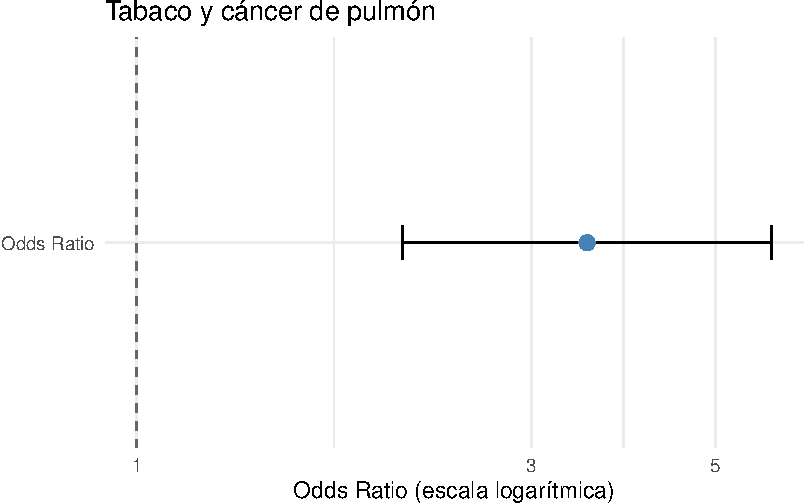
\includegraphics[keepaspectratio]{05-estudios-casos-controles_files/figure-pdf/forest-plot-or-1.pdf}}

}

\caption{Odds ratio del consumo de tabaco y su intervalo de confianza al
95\%.}

\end{figure}%

El punto se sitúa claramente a la derecha de la línea de referencia
\(OR=1\), y todo el intervalo de confianza queda también por encima de
ella, lo que confirma gráficamente que el consumo de tabaco está
asociado de forma significativa con un mayor riesgo de cáncer de pulmón
en esta muestra.

\section{Casos y controles apareados}\label{casos-y-controles-apareados}

En ocasiones, cada caso se \emph{aparea} (\emph{matching}) con uno o
varios controles que comparten con él ciertas características que se
sabe o se sospecha que actúan como factores de confusión, como la edad,
el sexo o el centro de reclutamiento. El objetivo del apareamiento es
asegurar que casos y controles sean lo más comparables posible en esas
variables, de forma que cualquier diferencia observada en la exposición
sea más difícilmente atribuible a ellas. Por ejemplo, a cada caso de 55
años se le podrían asignar dos controles también de 55 años y del mismo
sexo.

El apareamiento tiene, sin embargo, un coste analítico: la tabla
\(2\times 2\) simple ya no resulta válida para comparar los grupos,
porque las observaciones dejan de ser independientes (cada caso está
ligado a su control o controles concretos). El análisis de datos
apareados requiere métodos estadísticos específicos, como el
\textbf{test de McNemar} para el caso de un control por caso, o la
regresión logística condicional cuando hay varios controles por caso,
que quedan fuera del alcance de este capítulo introductorio.

\section{Cuándo utilizar este
diseño}\label{cuuxe1ndo-utilizar-este-diseuxf1o-3}

El estudio de casos y controles es la opción de elección cuando la
enfermedad o el evento de interés es raro, cuando su periodo de latencia
es muy largo, o cuando se dispone de poco tiempo y presupuesto para
completar la investigación. También resulta muy útil como paso
exploratorio para generar hipótesis sobre múltiples posibles
exposiciones a la vez, antes de invertir en un diseño más costoso.
Cuando, por el contrario, es la \textbf{exposición} la que resulta rara
en la población (y no la enfermedad), suele ser preferible recurrir a un
\hyperref[estudios-de-cohortes]{estudio de cohortes}, que garantiza un
número suficiente de expuestos y permite además calcular directamente
incidencias y riesgos relativos. En la práctica, ambos diseños se
consideran complementarios dentro de la investigación epidemiológica
observacional.

\chapter{Estudios ecológicos}\label{estudios-ecoluxf3gicos}

Todos los diseños vistos hasta ahora en este libro comparten un rasgo
común: la unidad de observación es el individuo. Sin embargo, no siempre
se dispone de datos a nivel individual, ni siempre interesa estudiarlos:
en ocasiones lo único disponible, o lo único relevante, son datos
agregados sobre grupos enteros de personas. El estudio ecológico es el
diseño observacional y analítico en el que la unidad de análisis no es
el individuo, sino un grupo o agregado de individuos (un país, una
región, un colegio, un periodo de tiempo), y en el que se relacionan
tasas o promedios agregados de exposición con tasas o promedios
agregados de resultado. Como se anticipó en el
\hyperref[introducciuxf3n-a-los-tipos-de-estudios-estaduxedsticos]{capítulo
de introducción}, este diseño ocupa una posición particular entre los
estudios analíticos, ya que permite generar hipótesis con gran rapidez
pero exige una cautela especial a la hora de interpretar sus resultados.

\section{Definición y
características}\label{definiciuxf3n-y-caracteruxedsticas-4}

\begin{definition}[Estudio
ecológico]\protect\hypertarget{def-ecologicos-estudio-ecologico}{}\label{def-ecologicos-estudio-ecologico}

Un \emph{estudio ecológico} es un estudio observacional y analítico en
el que la unidad de análisis es un grupo o agregado de individuos,
denominado \emph{unidad ecológica}, y en el que se estudia la relación
entre una medida agregada de exposición (una tasa, una proporción o una
media) y una medida agregada de resultado, calculadas ambas para cada
unidad ecológica.

\end{definition}

Lo que distingue a un estudio ecológico de todos los demás diseños de
este libro no es el tipo de medida que se calcula, sino la naturaleza de
la unidad de observación. En un estudio de cohortes o de casos y
controles, cada fila de la base de datos corresponde a una persona; en
un estudio ecológico, cada fila corresponde a un grupo, del que solo se
conocen valores resumidos (por ejemplo, el porcentaje de fumadores o la
tasa de mortalidad), y se ignora la combinación exacta de exposición y
resultado que presenta cada individuo del grupo.

Una \textbf{unidad ecológica} puede definirse de muy diversas formas,
dependiendo de la disponibilidad de datos agregados y de la pregunta de
investigación. Algunos ejemplos habituales son:

\begin{itemize}
\tightlist
\item
  \textbf{Áreas geográficas}: países, comunidades autónomas, provincias
  o municipios, para los que existen estadísticas oficiales agregadas
  (renta media, tasas de mortalidad, cobertura vacunal, etc.).
\item
  \textbf{Instituciones}: colegios, hospitales o empresas, comparados a
  partir de indicadores agregados de sus miembros (por ejemplo, el gasto
  medio por alumno y la tasa de graduación de cada colegio).
\item
  \textbf{Cohortes de nacimiento o periodos de tiempo}: grupos de
  personas nacidas en un mismo año, o datos agregados por años
  calendario, para estudiar tendencias temporales conjuntas de una
  exposición y un resultado.
\end{itemize}

\section{Ventajas e inconvenientes}\label{ventajas-e-inconvenientes-4}

\textbf{Ventajas}

\begin{itemize}
\tightlist
\item
  Es, con diferencia, uno de los diseños más rápidos y baratos de llevar
  a cabo, ya que habitualmente no requiere recoger datos nuevos.
\item
  Aprovecha datos agregados ya disponibles, como estadísticas oficiales,
  registros administrativos o indicadores publicados por organismos
  públicos, sin necesidad de reclutar y seguir a individuos.
\item
  Es muy útil para generar hipótesis de forma exploratoria, que después
  podrán confirmarse (o no) con diseños a nivel individual.
\item
  Permite estudiar exposiciones que solo tienen sentido a nivel de
  grupo, como políticas públicas, normativas, campañas o características
  del entorno, que no varían entre los individuos de una misma unidad
  ecológica.
\item
  Permite detectar \textbf{efectos contextuales}, es decir, efectos del
  grupo sobre el individuo que no pueden observarse estudiando
  únicamente características individuales (por ejemplo, el efecto de
  vivir en una región con mayor desigualdad de renta, con independencia
  de la renta propia de cada individuo).
\end{itemize}

\textbf{Inconvenientes}

\begin{itemize}
\tightlist
\item
  Al no disponer de datos individuales, no se puede saber si, dentro de
  cada unidad ecológica, son realmente los individuos expuestos los que
  presentan el resultado, o si exposición y resultado se distribuyen
  entre personas distintas del mismo grupo.
\item
  La falta de información individual impide controlar adecuadamente los
  factores de confusión a nivel de persona, que solo pueden ajustarse
  (si acaso) de forma agregada.
\item
  Los grupos comparados pueden diferir en muchas otras características
  además de la exposición estudiada, lo que dificulta atribuir la
  asociación observada a esa exposición concreta.
\item
  Su limitación más importante, hasta el punto de merecer un nombre
  propio, es la posibilidad de incurrir en una \textbf{falacia
  ecológica}, que se desarrolla con detalle en el apartado siguiente.
\end{itemize}

\section{Medidas propias de este
diseño}\label{medidas-propias-de-este-diseuxf1o-4}

La medida de asociación característica del estudio ecológico es el
coeficiente de correlación aplicado, no a datos individuales, sino a las
tasas o medias agregadas de las \(n\) unidades ecológicas comparadas.

\begin{definition}[Coeficiente de correlación
ecológica]\protect\hypertarget{def-ecologicos-correlacion-agregada}{}\label{def-ecologicos-correlacion-agregada}

Dadas \(n\) unidades ecológicas, para cada una de las cuales se dispone
de una medida agregada de exposición \(x_i\) (una tasa, proporción o
media) y una medida agregada de resultado \(y_i\), el \emph{coeficiente
de correlación ecológica} es el coeficiente de correlación de Pearson
calculado sobre esos \(n\) pares de valores agregados,

\[r = \frac{\displaystyle\sum_{i=1}^n (x_i-\bar x)(y_i-\bar y)}{\sqrt{\displaystyle\sum_{i=1}^n (x_i-\bar x)^2}\sqrt{\displaystyle\sum_{i=1}^n (y_i-\bar y)^2}}\]

donde \(\bar x\) y \(\bar y\) son las medias de las medidas agregadas de
exposición y de resultado, respectivamente, en las \(n\) unidades
ecológicas.

\end{definition}

\begin{tcolorbox}[enhanced jigsaw, arc=.35mm, bottomrule=.15mm, bottomtitle=1mm, breakable, colback=white, colbacktitle=quarto-callout-important-color!10!white, colframe=quarto-callout-important-color-frame, coltitle=black, left=2mm, leftrule=.75mm, opacityback=0, opacitybacktitle=0.6, rightrule=.15mm, title=\textcolor{quarto-callout-important-color}{\faExclamation}\hspace{0.5em}{Importante}, titlerule=0mm, toprule=.15mm, toptitle=1mm]

Al ser un coeficiente de correlación de Pearson, el coeficiente de
correlación ecológica siempre verifica

\[-1\leq r\leq 1.\]

\end{tcolorbox}

\begin{tcolorbox}[enhanced jigsaw, arc=.35mm, bottomrule=.15mm, bottomtitle=1mm, breakable, colback=white, colbacktitle=quarto-callout-note-color!10!white, colframe=quarto-callout-note-color-frame, coltitle=black, left=2mm, leftrule=.75mm, opacityback=0, opacitybacktitle=0.6, rightrule=.15mm, title=\textcolor{quarto-callout-note-color}{\faInfo}\hspace{0.5em}{Interpretación}, titlerule=0mm, toprule=.15mm, toptitle=1mm]

\begin{itemize}
\tightlist
\item
  El signo de \(r\) indica el sentido de la relación entre las unidades
  ecológicas: si \(r>0\), las unidades con mayor exposición agregada
  tienden a presentar también mayor resultado agregado; si \(r<0\),
  ocurre lo contrario.
\item
  Cuanto más se aproxima \(|r|\) a 1, más fuerte es la relación lineal
  observada entre las medidas agregadas.
\item
  Si \(r\) es próximo a 0, no se observa relación lineal entre la
  exposición y el resultado a nivel de las unidades ecológicas.
\item
  Es fundamental recordar que \(r\) mide una asociación \textbf{entre
  grupos}, no entre individuos, tal y como se explica a continuación.
\end{itemize}

\end{tcolorbox}

La principal amenaza a la validez de las conclusiones de un estudio
ecológico es la posibilidad de trasladar indebidamente una asociación
observada entre grupos a una afirmación sobre los individuos que los
componen.

\begin{definition}[Falacia
ecológica]\protect\hypertarget{def-ecologicos-falacia-ecologica}{}\label{def-ecologicos-falacia-ecologica}

La \emph{falacia ecológica} consiste en inferir, a partir de una
asociación observada entre la exposición y el resultado agregados a
nivel de grupo, que existe esa misma asociación entre la exposición y el
resultado a nivel individual, sin disponer de datos individuales que lo
confirmen.

\end{definition}

\begin{tcolorbox}[enhanced jigsaw, arc=.35mm, bottomrule=.15mm, bottomtitle=1mm, breakable, colback=white, colbacktitle=quarto-callout-warning-color!10!white, colframe=quarto-callout-warning-color-frame, coltitle=black, left=2mm, leftrule=.75mm, opacityback=0, opacitybacktitle=0.6, rightrule=.15mm, title=\textcolor{quarto-callout-warning-color}{\faExclamationTriangle}\hspace{0.5em}{Advertencia}, titlerule=0mm, toprule=.15mm, toptitle=1mm]

Una correlación ecológica alta \textbf{no implica} que, dentro de cada
unidad ecológica, sean precisamente los individuos expuestos los que
presenten el resultado. La asociación agregada puede deberse, total o
parcialmente, a diferencias entre grupos que nada tienen que ver con la
relación individual entre exposición y resultado, e incluso puede tener
signo contrario al de la verdadera asociación individual.

Un ejemplo clásico ilustra el problema: si se calcula, para cada
comunidad autónoma, el porcentaje de población nacida en el extranjero y
la tasa media de alfabetización, es posible encontrar una correlación
ecológica positiva (las comunidades con mayor proporción de población
extranjera presentan, en promedio, tasas de alfabetización más altas),
simplemente porque la población extranjera tiende a concentrarse en las
regiones más urbanas y con mejores sistemas educativos. Concluir de ahí
que, a nivel individual, las personas nacidas en el extranjero tienen
mayor probabilidad de saber leer y escribir que las nacidas en España
sería un error: los datos agregados no informan sobre qué personas
concretas, dentro de cada comunidad, son las que están alfabetizadas, y
la relación individual podría ser incluso la contraria.

\end{tcolorbox}

\begin{example}[]\protect\hypertarget{exm-ecologicos-correlacion-alcohol-cirrosis}{}\label{exm-ecologicos-correlacion-alcohol-cirrosis}

Se dispone de datos agregados de 7 países sobre el consumo medio de
alcohol per cápita (\(x\), en litros de alcohol puro al año) y la tasa
de mortalidad por cirrosis hepática (\(y\), casos por cada 100 000
habitantes):

\[
\begin{array}{lrrrrrrr}
\hline
\mbox{País} & x_i & y_i & x_i-\bar x & y_i-\bar y & (x_i-\bar x)(y_i-\bar y) & (x_i-\bar x)^2 & (y_i-\bar y)^2\\
\hline
\mbox{País 1} & 2 & 5 & -6 & -10 & 60 & 36 & 100\\
\mbox{País 2} & 4 & 8 & -4 & -7 & 28 & 16 & 49\\
\mbox{País 3} & 6 & 11 & -2 & -4 & 8 & 4 & 16\\
\mbox{País 4} & 8 & 15 & 0 & 0 & 0 & 0 & 0\\
\mbox{País 5} & 10 & 18 & 2 & 3 & 6 & 4 & 9\\
\mbox{País 6} & 12 & 20 & 4 & 5 & 20 & 16 & 25\\
\mbox{País 7} & 14 & 28 & 6 & 13 & 78 & 36 & 169\\
\hline
\mbox{Total} & 56 & 105 & & & 200 & 112 & 368\\
\hline
\end{array}
\]

Las medias agregadas son \(\bar x = 56/7 = 8\) litros y
\(\bar y = 105/7 = 15\) casos por cada 100 000 habitantes. Con las sumas
de la tabla, el coeficiente de correlación ecológica resulta

\[r = \frac{\sum (x_i-\bar x)(y_i-\bar y)}{\sqrt{\sum (x_i-\bar x)^2}\sqrt{\sum (y_i-\bar y)^2}} = \frac{200}{\sqrt{112}\sqrt{368}} = \frac{200}{203.02} \approx 0.985.\]

Existe, por tanto, una correlación ecológica positiva y muy fuerte entre
el consumo medio de alcohol y la mortalidad por cirrosis a nivel de
país: los países con mayor consumo agregado tienden a presentar también
una mayor tasa agregada de mortalidad por esta causa. Esta asociación es
coherente con lo que se sabe a nivel clínico sobre el alcohol y la
cirrosis, pero conviene insistir en que, por sí sola, esta correlación
agregada de 7 países no demuestra que sean los individuos que más beben
dentro de cada país los que fallecen por cirrosis: para eso haría falta
un diseño con datos individuales, como un
\hyperref[estudios-de-cohortes]{estudio de cohortes}.

\end{example}

\section{Realización con R}\label{realizaciuxf3n-con-r-4}

A continuación se construye un conjunto de datos agregados por región,
con el consumo medio diario de sal (\(x\), en gramos por persona y día)
y la tasa de hipertensión arterial (\(y\), casos por cada 1000
habitantes) de 18 regiones ficticias, tal y como podrían obtenerse a
partir de estadísticas sanitarias oficiales.

\begin{Shaded}
\begin{Highlighting}[]
\FunctionTok{set.seed}\NormalTok{(}\DecValTok{123}\NormalTok{)}

\NormalTok{n\_regiones }\OtherTok{\textless{}{-}} \DecValTok{18}

\NormalTok{datos\_ecologicos }\OtherTok{\textless{}{-}} \FunctionTok{tibble}\NormalTok{(}
  \AttributeTok{region =} \FunctionTok{paste}\NormalTok{(}\StringTok{"Región"}\NormalTok{, }\DecValTok{1}\SpecialCharTok{:}\NormalTok{n\_regiones),}
  \AttributeTok{consumo\_sal =} \FunctionTok{round}\NormalTok{(}\FunctionTok{rnorm}\NormalTok{(n\_regiones, }\AttributeTok{mean =} \DecValTok{8}\NormalTok{, }\AttributeTok{sd =} \FloatTok{1.8}\NormalTok{), }\DecValTok{1}\NormalTok{)}
\NormalTok{) }\SpecialCharTok{|\textgreater{}}
  \FunctionTok{mutate}\NormalTok{(}
    \AttributeTok{tasa\_hipertension =} \FunctionTok{round}\NormalTok{(}\DecValTok{15} \SpecialCharTok{+} \DecValTok{6} \SpecialCharTok{*}\NormalTok{ consumo\_sal }\SpecialCharTok{+} \FunctionTok{rnorm}\NormalTok{(n\_regiones, }\AttributeTok{mean =} \DecValTok{0}\NormalTok{, }\AttributeTok{sd =} \DecValTok{10}\NormalTok{), }\DecValTok{1}\NormalTok{)}
\NormalTok{  )}

\NormalTok{datos\_ecologicos}
\end{Highlighting}
\end{Shaded}

\begin{verbatim}
# A tibble: 18 x 3
   region    consumo_sal tasa_hipertension
   <chr>           <dbl>             <dbl>
 1 Región 1          7                64  
 2 Región 2          7.6              55.9
 3 Región 3         10.8              69.1
 4 Región 4          8.1              61.4
 5 Región 5          8.2              53.9
 6 Región 6         11.1              74.3
 7 Región 7          8.8              61.5
 8 Región 8          5.7              32.3
 9 Región 9          6.8              64.2
10 Región 10         7.2              59.7
11 Región 11        10.2              64.8
12 Región 12         8.6              79.1
13 Región 13         8.7              71.5
14 Región 14         8.2              61.2
15 Región 15         7                66  
16 Región 16        11.2              91  
17 Región 17         8.9              76.6
18 Región 18         4.5              48.9
\end{verbatim}

Cada fila representa una región completa, no una persona:
\texttt{consumo\_sal} es el consumo medio agregado de esa región, y
\texttt{tasa\_hipertension} es la tasa agregada de hipertensión en esa
misma región.

El coeficiente de correlación ecológica entre ambas variables agregadas
se calcula con \texttt{cor()}, y su significación estadística con
\texttt{cor.test()}:

\begin{Shaded}
\begin{Highlighting}[]
\NormalTok{correlacion }\OtherTok{\textless{}{-}} \FunctionTok{cor}\NormalTok{(datos\_ecologicos}\SpecialCharTok{$}\NormalTok{consumo\_sal, datos\_ecologicos}\SpecialCharTok{$}\NormalTok{tasa\_hipertension)}
\NormalTok{correlacion}
\end{Highlighting}
\end{Shaded}

\begin{verbatim}
[1] 0.7283621
\end{verbatim}

\begin{Shaded}
\begin{Highlighting}[]
\NormalTok{test\_correlacion }\OtherTok{\textless{}{-}} \FunctionTok{cor.test}\NormalTok{(datos\_ecologicos}\SpecialCharTok{$}\NormalTok{consumo\_sal, datos\_ecologicos}\SpecialCharTok{$}\NormalTok{tasa\_hipertension)}
\NormalTok{test\_correlacion}
\end{Highlighting}
\end{Shaded}

\begin{verbatim}

    Pearson's product-moment correlation

data:  datos_ecologicos$consumo_sal and datos_ecologicos$tasa_hipertension
t = 4.252, df = 16, p-value = 0.0006086
alternative hypothesis: true correlation is not equal to 0
95 percent confidence interval:
 0.3962304 0.8919307
sample estimates:
      cor 
0.7283621 
\end{verbatim}

El coeficiente de correlación ecológica es 0.73, lo que indica una
asociación positiva y fuerte entre el consumo medio de sal y la tasa de
hipertensión a nivel regional, y el contraste de hipótesis asociado
sugiere que esta correlación es difícilmente atribuible al azar.

A continuación se ajusta una recta de regresión sobre los datos
agregados con \texttt{lm()}:

\begin{Shaded}
\begin{Highlighting}[]
\NormalTok{modelo\_ecologico }\OtherTok{\textless{}{-}} \FunctionTok{lm}\NormalTok{(tasa\_hipertension }\SpecialCharTok{\textasciitilde{}}\NormalTok{ consumo\_sal, }\AttributeTok{data =}\NormalTok{ datos\_ecologicos)}
\FunctionTok{summary}\NormalTok{(modelo\_ecologico)}
\end{Highlighting}
\end{Shaded}

\begin{verbatim}

Call:
lm(formula = tasa_hipertension ~ consumo_sal, data = datos_ecologicos)

Residuals:
    Min      1Q  Median      3Q     Max 
-18.794  -5.341  -0.536   7.163  13.146 

Coefficients:
            Estimate Std. Error t value Pr(>|t|)    
(Intercept)   21.887     10.171   2.152 0.047028 *  
consumo_sal    5.124      1.205   4.252 0.000609 ***
---
Signif. codes:  0 '***' 0.001 '**' 0.01 '*' 0.05 '.' 0.1 ' ' 1

Residual standard error: 8.98 on 16 degrees of freedom
Multiple R-squared:  0.5305,    Adjusted R-squared:  0.5012 
F-statistic: 18.08 on 1 and 16 DF,  p-value: 0.0006086
\end{verbatim}

Y se representa el diagrama de dispersión de las 18 regiones junto con
la recta de regresión ajustada:

\begin{Shaded}
\begin{Highlighting}[]
\FunctionTok{ggplot}\NormalTok{(datos\_ecologicos, }\FunctionTok{aes}\NormalTok{(}\AttributeTok{x =}\NormalTok{ consumo\_sal, }\AttributeTok{y =}\NormalTok{ tasa\_hipertension)) }\SpecialCharTok{+}
  \FunctionTok{geom\_point}\NormalTok{(}\AttributeTok{size =} \DecValTok{3}\NormalTok{, }\AttributeTok{color =} \StringTok{"steelblue"}\NormalTok{) }\SpecialCharTok{+}
  \FunctionTok{geom\_smooth}\NormalTok{(}\AttributeTok{method =} \StringTok{"lm"}\NormalTok{, }\AttributeTok{se =} \ConstantTok{TRUE}\NormalTok{, }\AttributeTok{color =} \StringTok{"firebrick"}\NormalTok{) }\SpecialCharTok{+}
  \FunctionTok{labs}\NormalTok{(}
    \AttributeTok{x =} \StringTok{"Consumo medio de sal (g/día)"}\NormalTok{,}
    \AttributeTok{y =} \StringTok{"Tasa de hipertensión (casos por 1000 hab.)"}\NormalTok{,}
    \AttributeTok{title =} \StringTok{"Correlación ecológica entre consumo de sal e hipertensión"}
\NormalTok{  ) }\SpecialCharTok{+}
  \FunctionTok{theme\_minimal}\NormalTok{()}
\end{Highlighting}
\end{Shaded}

\begin{figure}[H]

{\centering \pandocbounded{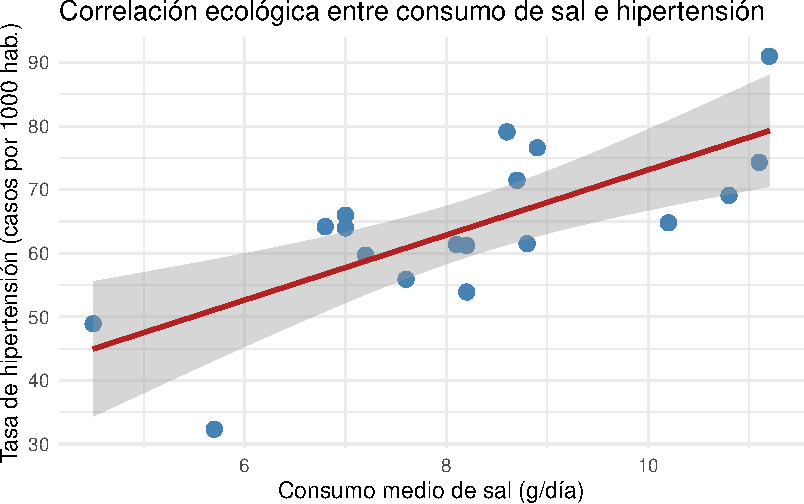
\includegraphics[keepaspectratio]{06-estudios-ecologicos_files/figure-pdf/grafico-dispersion-1.pdf}}

}

\caption{Relación ecológica entre el consumo medio de sal y la tasa de
hipertensión en 18 regiones.}

\end{figure}%

Cada punto del gráfico representa una región entera, no una persona. La
nube de puntos y la recta ajustada muestran una relación positiva clara
entre el consumo medio de sal y la tasa de hipertensión a nivel
regional: las regiones que, en promedio, consumen más sal presentan
también, en promedio, tasas de hipertensión más altas. Sin embargo,
estos datos agregados no permiten afirmar que sean precisamente las
personas que más sal consumen, dentro de cada región, las que
desarrollan hipertensión: podría haber diferencias entre regiones (edad
media de la población, acceso a la sanidad, otros hábitos dietéticos)
que expliquen parte de esta asociación agregada, y la propia falacia
ecológica advierte de que la relación a nivel individual debería
confirmarse con un diseño que recoja datos de cada persona.

\section{Cuándo utilizar este
diseño}\label{cuuxe1ndo-utilizar-este-diseuxf1o-4}

El estudio ecológico resulta especialmente útil como primera
aproximación rápida y económica a una pregunta de investigación, cuando
ya existen estadísticas agregadas disponibles y no es viable, al menos
en una fase inicial, recoger datos a nivel individual. También es el
diseño de elección, y en muchos casos el único posible, cuando la
exposición que se quiere estudiar es en sí misma una característica de
grupo (una política sanitaria, una normativa medioambiental, una campaña
de salud pública) que no varía entre los individuos de una misma unidad
ecológica y que, por tanto, no podría analizarse comparando personas
dentro de un mismo grupo. Sin embargo, precisamente por la amenaza de la
falacia ecológica, cualquier asociación encontrada con este diseño debe
tratarse como una hipótesis preliminar, no como una conclusión
establecida. Cuando el objetivo final es determinar si la exposición y
el resultado están realmente asociados a nivel de persona, es necesario
confirmar los hallazgos ecológicos con un diseño que recoja datos
individuales, como un \hyperref[estudios-de-cohortes]{estudio de
cohortes} o un \hyperref[estudios-de-casos-y-controles]{estudio de casos
y controles}, antes de trasladar las conclusiones a los individuos.

\chapter{Estudios experimentales}\label{estudios-experimentales}

A diferencia de los diseños observacionales estudiados en los capítulos
anteriores, en los que el investigador se limita a observar lo que
ocurre de forma natural, en un \emph{estudio experimental} es el propio
investigador quien decide, de forma activa, qué tratamiento o exposición
recibe cada individuo. Esta capacidad de intervenir sobre la exposición,
unida a la asignación aleatoria de los sujetos a los distintos grupos,
convierte al estudio experimental en el diseño con mayor capacidad para
establecer relaciones causales de todos los vistos hasta ahora. Dentro
de los estudios experimentales, el \emph{ensayo clínico aleatorizado}
es, con diferencia, el más utilizado, especialmente en la evaluación de
nuevos fármacos y tratamientos, y constituye el paradigma de este tipo
de diseño. Los conceptos generales de estudio experimental frente a
observacional se presentaron en el
\hyperref[introducciuxf3n-a-los-tipos-de-estudios-estaduxedsticos]{capítulo
de introducción}.

\section{Definición y
características}\label{definiciuxf3n-y-caracteruxedsticas-5}

\begin{definition}[Ensayo clínico
aleatorizado]\protect\hypertarget{def-experimentales-ensayo-clinico-aleatorizado}{}\label{def-experimentales-ensayo-clinico-aleatorizado}

Un \emph{ensayo clínico aleatorizado} (ECA) es un estudio experimental,
analítico y longitudinal en el que un grupo de individuos se asigna al
azar a recibir un tratamiento (o exposición) experimental o un
tratamiento de control, y se les sigue en el tiempo para comparar la
frecuencia con la que se produce el resultado de interés en ambos
grupos.

\end{definition}

El ensayo clínico aleatorizado comparte con el estudio de cohortes la
lógica general (se parte de la exposición y se observa el resultado a lo
largo del tiempo), pero se diferencia de él en un aspecto esencial:
mientras que en el estudio de cohortes la exposición la determinan los
propios individuos o las circunstancias, en el ensayo clínico es el
investigador quien la asigna, y además lo hace de forma aleatoria. Esta
doble característica, intervención y aleatorización, es la que dota a
este diseño de su extraordinaria capacidad para el control de los
factores de confusión. Tres elementos son clave en su diseño: la
aleatorización, la existencia de un grupo control (habitualmente con
placebo) y el cegamiento.

\subsection{Aleatorización}\label{aleatorizaciuxf3n}

\begin{definition}[Aleatorización]\protect\hypertarget{def-experimentales-aleatorizacion}{}\label{def-experimentales-aleatorizacion}

La \emph{aleatorización} es el procedimiento por el cual la asignación
de cada individuo al grupo experimental o al grupo control se realiza
mediante un mecanismo puramente aleatorio (por ejemplo, un generador de
números aleatorios), de forma que todos los individuos tienen la misma
probabilidad de recibir cada uno de los tratamientos.

\end{definition}

\begin{tcolorbox}[enhanced jigsaw, arc=.35mm, bottomrule=.15mm, bottomtitle=1mm, breakable, colback=white, colbacktitle=quarto-callout-important-color!10!white, colframe=quarto-callout-important-color-frame, coltitle=black, left=2mm, leftrule=.75mm, opacityback=0, opacitybacktitle=0.6, rightrule=.15mm, title=\textcolor{quarto-callout-important-color}{\faExclamation}\hspace{0.5em}{Importante}, titlerule=0mm, toprule=.15mm, toptitle=1mm]

Si el proceso de asignación es realmente aleatorio y el tamaño muestral
es suficientemente grande, la aleatorización tiende a repartir por igual
entre los grupos tanto los factores de confusión conocidos por el
investigador como los que no lo son (o los que ni siquiera se han
llegado a identificar). Esto es algo que ningún diseño observacional
puede garantizar, por muy cuidadoso que sea el ajuste estadístico
posterior, ya que este solo puede corregir el efecto de las variables
que se han medido.

\end{tcolorbox}

\begin{tcolorbox}[enhanced jigsaw, arc=.35mm, bottomrule=.15mm, bottomtitle=1mm, breakable, colback=white, colbacktitle=quarto-callout-note-color!10!white, colframe=quarto-callout-note-color-frame, coltitle=black, left=2mm, leftrule=.75mm, opacityback=0, opacitybacktitle=0.6, rightrule=.15mm, title=\textcolor{quarto-callout-note-color}{\faInfo}\hspace{0.5em}{Interpretación}, titlerule=0mm, toprule=.15mm, toptitle=1mm]

Gracias a la aleatorización, si al final del estudio se observa una
diferencia en el resultado entre los dos grupos, esa diferencia puede
atribuirse con mucha mayor confianza al tratamiento y no a otras
características previas de los individuos, ya que estas se distribuyen
de forma similar (en promedio) en ambos grupos.

\end{tcolorbox}

\subsection{Grupo control y placebo}\label{grupo-control-y-placebo}

En todo ensayo clínico es necesario disponer de un grupo de comparación,
el \emph{grupo control}, que permite valorar qué le hubiera ocurrido a
los individuos del grupo experimental si no hubieran recibido el
tratamiento en estudio. Sin este grupo de referencia sería imposible
saber si la evolución observada en los pacientes tratados se debe al
tratamiento o a otros factores, como la evolución natural de la
enfermedad.

El grupo control puede recibir un \emph{placebo} (una sustancia o
procedimiento inactivo, sin efecto farmacológico, pero indistinguible
del tratamiento experimental en apariencia) cuando no existe un
tratamiento eficaz conocido para la enfermedad estudiada, o bien el
\emph{tratamiento estándar} ya disponible, cuando por motivos éticos no
seria admisible dejar sin tratamiento a los pacientes del grupo control.
En ambos casos el objetivo es el mismo: aislar el efecto específico del
nuevo tratamiento del efecto inespecífico de recibir cualquier atención
o intervención.

\subsection{Cegamiento}\label{cegamiento}

\begin{definition}[Cegamiento]\protect\hypertarget{def-experimentales-cegamiento}{}\label{def-experimentales-cegamiento}

El \emph{cegamiento} (o enmascaramiento) es el procedimiento por el cual
se oculta a los participantes, a los investigadores, o a ambos, qué
tratamiento está recibiendo cada individuo, con el fin de evitar que ese
conocimiento influya en el resultado del estudio.

\end{definition}

Se distinguen varios niveles de cegamiento:

\begin{itemize}
\tightlist
\item
  En un ensayo \emph{simple ciego}, el paciente desconoce si recibe el
  tratamiento experimental o el control, pero el investigador sí lo
  sabe.
\item
  En un ensayo \emph{doble ciego}, ni el paciente ni el investigador que
  evalúa el resultado conocen el tratamiento asignado.
\item
  En un ensayo \emph{abierto} no existe cegamiento: tanto el paciente
  como el investigador conocen el tratamiento asignado, algo inevitable
  en algunos diseños (por ejemplo, cuando se compara cirugía frente a
  tratamiento farmacológico).
\end{itemize}

\begin{tcolorbox}[enhanced jigsaw, arc=.35mm, bottomrule=.15mm, bottomtitle=1mm, breakable, colback=white, colbacktitle=quarto-callout-note-color!10!white, colframe=quarto-callout-note-color-frame, coltitle=black, left=2mm, leftrule=.75mm, opacityback=0, opacitybacktitle=0.6, rightrule=.15mm, title=\textcolor{quarto-callout-note-color}{\faInfo}\hspace{0.5em}{Interpretación}, titlerule=0mm, toprule=.15mm, toptitle=1mm]

El cegamiento reduce el sesgo de información en ambas direcciones: evita
que el conocimiento del tratamiento modifique la respuesta del paciente
(por ejemplo, mediante el efecto placebo, o comunicando síntomas de
forma distinta según lo que espera sentir) y evita que el investigador,
de forma consciente o inconsciente, valore el resultado de forma
diferente según el tratamiento que sabe que ha recibido cada paciente.

\end{tcolorbox}

\section{Ventajas e inconvenientes}\label{ventajas-e-inconvenientes-5}

El ensayo clínico aleatorizado presenta ventajas muy destacadas frente
al resto de diseños estudiados hasta ahora:

\begin{itemize}
\tightlist
\item
  Proporciona la evidencia más sólida para establecer relaciones de
  causalidad entre una exposición o tratamiento y un resultado, por lo
  que se considera el patrón de referencia (\emph{gold standard}) de la
  investigación clínica.
\item
  La aleatorización controla simultáneamente los factores de confusión
  conocidos y los desconocidos, algo que ningún estudio observacional
  puede lograr.
\item
  El investigador controla el momento y la forma en que se administra la
  exposición, lo que reduce muchos de los sesgos de selección e
  información habituales en los estudios observacionales.
\item
  El cegamiento y el uso de un grupo control con placebo permiten aislar
  el efecto específico del tratamiento.
\end{itemize}

Frente a estas ventajas, el diseño presenta también inconvenientes
importantes:

\begin{itemize}
\tightlist
\item
  Suele requerir un coste económico y una duración muy elevados, sobre
  todo cuando el resultado de interés tarda mucho tiempo en manifestarse
  o es poco frecuente.
\item
  Plantea problemas éticos que limitan notablemente su aplicabilidad: no
  es aceptable asignar de forma aleatoria una exposición que se sospecha
  perjudicial, ni negar a un grupo de pacientes un tratamiento del que
  ya existe evidencia de eficacia.
\item
  Los criterios de inclusión y exclusión, necesarios para garantizar la
  seguridad de los participantes y la homogeneidad de la muestra, suelen
  ser muy estrictos, lo que limita la validez externa (la capacidad de
  generalizar los resultados a la población general de pacientes, más
  heterogénea que la muestra del ensayo).
\end{itemize}

\section{Medidas propias de este
diseño}\label{medidas-propias-de-este-diseuxf1o-5}

Al igual que en el estudio de cohortes, en un ensayo clínico se comparan
las incidencias del resultado de interés en el grupo experimental y en
el grupo control, a partir de una tabla de contingencia como la
siguiente, donde \(a\) y \(c\) son el número de individuos en los que se
produce el evento en el grupo experimental y en el grupo control,
respectivamente, y \(n_e\) y \(n_c\) el número total de individuos en
cada grupo:

\[
\begin{array}{lrrr}
\hline
 & \mbox{Evento} & \mbox{No evento} & \mbox{Total}\\
\hline
\mbox{Experimental} & a & b & n_e\\
\mbox{Control} & c & d & n_c\\
\hline
\end{array}
\]

A partir de esta tabla se define la incidencia del evento en el grupo
experimental, \(I_e = a/n_e\), y la incidencia del evento en el grupo
control, \(I_c = c/n_c\). Sobre estas dos incidencias se construyen tres
medidas propias de este diseño, especialmente utilizadas cuando el
resultado de interés es un evento adverso que el tratamiento pretende
evitar: la reducción relativa del riesgo, la reducción absoluta del
riesgo y el número necesario a tratar.

\subsection{Reducción relativa del
riesgo}\label{reducciuxf3n-relativa-del-riesgo}

\begin{definition}[Reducción relativa del
riesgo]\protect\hypertarget{def-experimentales-rrr}{}\label{def-experimentales-rrr}

La \emph{reducción relativa del riesgo} (RRR) es la proporción en la que
el tratamiento experimental reduce el riesgo del evento respecto al
grupo control, y se define como

\[RRR = \frac{I_c - I_e}{I_c}\]

\end{definition}

\begin{tcolorbox}[enhanced jigsaw, arc=.35mm, bottomrule=.15mm, bottomtitle=1mm, breakable, colback=white, colbacktitle=quarto-callout-important-color!10!white, colframe=quarto-callout-important-color-frame, coltitle=black, left=2mm, leftrule=.75mm, opacityback=0, opacitybacktitle=0.6, rightrule=.15mm, title=\textcolor{quarto-callout-important-color}{\faExclamation}\hspace{0.5em}{Importante}, titlerule=0mm, toprule=.15mm, toptitle=1mm]

Cuando el tratamiento experimental reduce el riesgo del evento respecto
al control (\(I_e < I_c\)), se tiene que

\[0 < RRR \leq 1,\]

y suele expresarse en tanto por ciento.

\end{tcolorbox}

\begin{tcolorbox}[enhanced jigsaw, arc=.35mm, bottomrule=.15mm, bottomtitle=1mm, breakable, colback=white, colbacktitle=quarto-callout-note-color!10!white, colframe=quarto-callout-note-color-frame, coltitle=black, left=2mm, leftrule=.75mm, opacityback=0, opacitybacktitle=0.6, rightrule=.15mm, title=\textcolor{quarto-callout-note-color}{\faInfo}\hspace{0.5em}{Interpretación}, titlerule=0mm, toprule=.15mm, toptitle=1mm]

Un \(RRR = 0.3\) (30\%) indica que el tratamiento experimental reduce el
riesgo de sufrir el evento en un 30\% respecto al riesgo del grupo
control. La reducción relativa del riesgo es equivalente a \(1-RR\),
donde \(RR=I_e/I_c\) es el riesgo relativo definido en el estudio de
cohortes, por lo que comparte con él la limitación de no informar sobre
la magnitud absoluta del riesgo evitado.

\end{tcolorbox}

\subsection{Reducción absoluta del
riesgo}\label{reducciuxf3n-absoluta-del-riesgo}

\begin{definition}[Reducción absoluta del
riesgo]\protect\hypertarget{def-experimentales-rar}{}\label{def-experimentales-rar}

La \emph{reducción absoluta del riesgo} (RAR) es la diferencia entre la
incidencia del evento en el grupo control y la incidencia del evento en
el grupo experimental, y se define como

\[RAR = I_c - I_e\]

\end{definition}

\begin{tcolorbox}[enhanced jigsaw, arc=.35mm, bottomrule=.15mm, bottomtitle=1mm, breakable, colback=white, colbacktitle=quarto-callout-important-color!10!white, colframe=quarto-callout-important-color-frame, coltitle=black, left=2mm, leftrule=.75mm, opacityback=0, opacitybacktitle=0.6, rightrule=.15mm, title=\textcolor{quarto-callout-important-color}{\faExclamation}\hspace{0.5em}{Importante}, titlerule=0mm, toprule=.15mm, toptitle=1mm]

Cuando el tratamiento experimental reduce el riesgo del evento respecto
al control (\(I_e < I_c\)), se tiene que

\[0 < RAR \leq 1.\]

\end{tcolorbox}

\begin{tcolorbox}[enhanced jigsaw, arc=.35mm, bottomrule=.15mm, bottomtitle=1mm, breakable, colback=white, colbacktitle=quarto-callout-note-color!10!white, colframe=quarto-callout-note-color-frame, coltitle=black, left=2mm, leftrule=.75mm, opacityback=0, opacitybacktitle=0.6, rightrule=.15mm, title=\textcolor{quarto-callout-note-color}{\faInfo}\hspace{0.5em}{Interpretación}, titlerule=0mm, toprule=.15mm, toptitle=1mm]

A diferencia de la reducción relativa, la reducción absoluta del riesgo
depende directamente del riesgo basal del grupo control: dos
tratamientos pueden tener la misma \(RRR\) y una \(RAR\) muy distinta si
las incidencias de partida son muy diferentes, por lo que la RAR ofrece
una idea más realista del beneficio esperado del tratamiento en la
práctica.

\end{tcolorbox}

\subsection{Número necesario a
tratar}\label{nuxfamero-necesario-a-tratar}

\begin{definition}[Número necesario a
tratar]\protect\hypertarget{def-experimentales-nnt}{}\label{def-experimentales-nnt}

El \emph{número necesario a tratar} (NNT) es el número de pacientes que
sería necesario tratar con el tratamiento experimental, en lugar de con
el control, para evitar un caso adicional del evento de interés, y se
define como el inverso de la reducción absoluta del riesgo:

\[NNT = \frac{1}{RAR}\]

\end{definition}

\begin{tcolorbox}[enhanced jigsaw, arc=.35mm, bottomrule=.15mm, bottomtitle=1mm, breakable, colback=white, colbacktitle=quarto-callout-note-color!10!white, colframe=quarto-callout-note-color-frame, coltitle=black, left=2mm, leftrule=.75mm, opacityback=0, opacitybacktitle=0.6, rightrule=.15mm, title=\textcolor{quarto-callout-note-color}{\faInfo}\hspace{0.5em}{Interpretación}, titlerule=0mm, toprule=.15mm, toptitle=1mm]

El NNT traduce la reducción absoluta del riesgo a una escala muy
intuitiva para la práctica clínica: un \(NNT=10\) significa que, de
media, hay que tratar a 10 pacientes con el nuevo tratamiento en lugar
de con el control para evitar que uno de ellos sufra el evento. Cuanto
menor es el NNT, mayor es la eficacia práctica del tratamiento.

\end{tcolorbox}

\begin{tcolorbox}[enhanced jigsaw, arc=.35mm, bottomrule=.15mm, bottomtitle=1mm, breakable, colback=white, colbacktitle=quarto-callout-warning-color!10!white, colframe=quarto-callout-warning-color-frame, coltitle=black, left=2mm, leftrule=.75mm, opacityback=0, opacitybacktitle=0.6, rightrule=.15mm, title=\textcolor{quarto-callout-warning-color}{\faExclamationTriangle}\hspace{0.5em}{Advertencia}, titlerule=0mm, toprule=.15mm, toptitle=1mm]

El NNT se calcula siempre como el inverso de la RAR expresada en
proporción (no en porcentaje) y, puesto que en la práctica no tiene
sentido tratar a una fracción de paciente, el resultado se redondea
siempre al entero superior (por ejemplo, un \(NNT=8.3\) se interpreta y
se comunica como \(NNT=9\)). Además, al depender de la RAR, el NNT no es
una propiedad fija del tratamiento, sino que varía con el riesgo basal
de la población a la que se aplique: el mismo tratamiento tendrá un NNT
mucho más favorable en pacientes de alto riesgo que en pacientes de bajo
riesgo, por lo que no debe extrapolarse sin más de una población a otra.

\end{tcolorbox}

\subsection{Ejemplo numérico}\label{ejemplo-numuxe9rico-1}

\begin{example}[]\protect\hypertarget{exm-experimentales-rrr-rar-nnt}{}\label{exm-experimentales-rrr-rar-nnt}

Se lleva a cabo un ensayo clínico aleatorizado, doble ciego y controlado
con placebo, para evaluar si un nuevo fármaco reduce la aparición de
infarto de miocardio en pacientes con alto riesgo cardiovascular. Se
reclutan 500 pacientes, que se asignan aleatoriamente a dos grupos de
250: uno recibe el fármaco experimental y otro recibe un placebo, y se
les sigue durante 3 años. Al finalizar el seguimiento se obtiene la
siguiente tabla de frecuencias:

\[
\begin{array}{lrrr}
\hline
 & \mbox{Infarto} & \mbox{No infarto} & \mbox{Total}\\
\hline
\mbox{Fármaco} & 25 & 225 & 250\\
\mbox{Placebo} & 50 & 200 & 250\\
\hline
\end{array}
\]

\textbf{Incidencias.} La incidencia de infarto en el grupo experimental
es

\[I_e = \frac{25}{250} = 0.10 = 10\%,\]

y la incidencia de infarto en el grupo control es

\[I_c = \frac{50}{250} = 0.20 = 20\%.\]

\textbf{Reducción relativa del riesgo.}

\[RRR = \frac{I_c - I_e}{I_c} = \frac{0.20 - 0.10}{0.20} = 0.5 = 50\%.\]

El fármaco reduce el riesgo de sufrir un infarto en un 50\% respecto al
riesgo de los pacientes que reciben placebo.

\textbf{Reducción absoluta del riesgo.}

\[RAR = I_c - I_e = 0.20 - 0.10 = 0.10 = 10\%.\]

De cada 100 pacientes tratados con el fármaco, se evitan 10 infartos que
sí se habrían producido de haber recibido placebo.

\textbf{Número necesario a tratar.}

\[NNT = \frac{1}{RAR} = \frac{1}{0.10} = 10.\]

Es necesario tratar a 10 pacientes con el nuevo fármaco, en lugar de con
placebo, durante 3 años, para evitar un infarto de miocardio adicional.
Obsérvese que, a pesar de que la reducción relativa del riesgo parece
muy elevada (50\%), el NNT permite valorar el beneficio del tratamiento
en términos absolutos y directamente aplicables a la práctica clínica.

\end{example}

\section{Realización con R}\label{realizaciuxf3n-con-r-5}

\subsection{Cálculo de las medidas a partir de la tabla de
contingencia}\label{cuxe1lculo-de-las-medidas-a-partir-de-la-tabla-de-contingencia-1}

El primer paso es reproducir con R el cálculo manual del ejemplo
anterior, construyendo la tabla de contingencia como una matriz y
calculando a partir de ella las incidencias, la RRR, la RAR y el NNT.

\begin{Shaded}
\begin{Highlighting}[]
\CommentTok{\# Tabla de contingencia: filas = grupo, columnas = resultado (infarto, no infarto)}
\NormalTok{tabla }\OtherTok{\textless{}{-}} \FunctionTok{matrix}\NormalTok{(}\FunctionTok{c}\NormalTok{(}\DecValTok{25}\NormalTok{, }\DecValTok{225}\NormalTok{, }\DecValTok{50}\NormalTok{, }\DecValTok{200}\NormalTok{),}
                 \AttributeTok{nrow =} \DecValTok{2}\NormalTok{, }\AttributeTok{byrow =} \ConstantTok{TRUE}\NormalTok{,}
                 \AttributeTok{dimnames =} \FunctionTok{list}\NormalTok{(}\AttributeTok{Grupo =} \FunctionTok{c}\NormalTok{(}\StringTok{"Farmaco"}\NormalTok{, }\StringTok{"Placebo"}\NormalTok{),}
                                  \AttributeTok{Resultado =} \FunctionTok{c}\NormalTok{(}\StringTok{"Infarto"}\NormalTok{, }\StringTok{"No infarto"}\NormalTok{)))}
\NormalTok{tabla}
\end{Highlighting}
\end{Shaded}

\begin{verbatim}
         Resultado
Grupo     Infarto No infarto
  Farmaco      25        225
  Placebo      50        200
\end{verbatim}

\begin{Shaded}
\begin{Highlighting}[]
\CommentTok{\# Incidencias del evento en cada grupo}
\NormalTok{i\_e }\OtherTok{\textless{}{-}}\NormalTok{ tabla[}\StringTok{"Farmaco"}\NormalTok{, }\StringTok{"Infarto"}\NormalTok{] }\SpecialCharTok{/} \FunctionTok{sum}\NormalTok{(tabla[}\StringTok{"Farmaco"}\NormalTok{, ])}
\NormalTok{i\_c }\OtherTok{\textless{}{-}}\NormalTok{ tabla[}\StringTok{"Placebo"}\NormalTok{, }\StringTok{"Infarto"}\NormalTok{] }\SpecialCharTok{/} \FunctionTok{sum}\NormalTok{(tabla[}\StringTok{"Placebo"}\NormalTok{, ])}
\FunctionTok{c}\NormalTok{(}\AttributeTok{I\_e =}\NormalTok{ i\_e, }\AttributeTok{I\_c =}\NormalTok{ i\_c)}
\end{Highlighting}
\end{Shaded}

\begin{verbatim}
I_e I_c 
0.1 0.2 
\end{verbatim}

\begin{Shaded}
\begin{Highlighting}[]
\CommentTok{\# Reducción relativa del riesgo, reducción absoluta del riesgo y NNT}
\NormalTok{rrr }\OtherTok{\textless{}{-}}\NormalTok{ (i\_c }\SpecialCharTok{{-}}\NormalTok{ i\_e) }\SpecialCharTok{/}\NormalTok{ i\_c}
\NormalTok{rar }\OtherTok{\textless{}{-}}\NormalTok{ i\_c }\SpecialCharTok{{-}}\NormalTok{ i\_e}
\NormalTok{nnt }\OtherTok{\textless{}{-}} \DecValTok{1} \SpecialCharTok{/}\NormalTok{ rar}
\FunctionTok{c}\NormalTok{(}\AttributeTok{RRR =}\NormalTok{ rrr, }\AttributeTok{RAR =}\NormalTok{ rar, }\AttributeTok{NNT =} \FunctionTok{ceiling}\NormalTok{(nnt))}
\end{Highlighting}
\end{Shaded}

\begin{verbatim}
 RRR  RAR  NNT 
 0.5  0.1 10.0 
\end{verbatim}

Los resultados, \(I_e=0.10\), \(I_c=0.20\), \(RRR=0.5\), \(RAR=0.10\) y
\(NNT=10\), coinciden exactamente con los obtenidos a mano.

Para representar gráficamente la diferencia entre grupos conviene
acompañar las incidencias observadas de su intervalo de confianza, que
puede obtenerse para cada grupo con \texttt{prop.test()}:

\begin{Shaded}
\begin{Highlighting}[]
\NormalTok{ic\_farmaco }\OtherTok{\textless{}{-}} \FunctionTok{prop.test}\NormalTok{(tabla[}\StringTok{"Farmaco"}\NormalTok{, }\StringTok{"Infarto"}\NormalTok{], }\FunctionTok{sum}\NormalTok{(tabla[}\StringTok{"Farmaco"}\NormalTok{, ]))}
\NormalTok{ic\_placebo }\OtherTok{\textless{}{-}} \FunctionTok{prop.test}\NormalTok{(tabla[}\StringTok{"Placebo"}\NormalTok{, }\StringTok{"Infarto"}\NormalTok{], }\FunctionTok{sum}\NormalTok{(tabla[}\StringTok{"Placebo"}\NormalTok{, ]))}

\NormalTok{incidencias }\OtherTok{\textless{}{-}} \FunctionTok{tibble}\NormalTok{(}
  \AttributeTok{grupo =} \FunctionTok{c}\NormalTok{(}\StringTok{"Fármaco"}\NormalTok{, }\StringTok{"Placebo"}\NormalTok{),}
  \AttributeTok{incidencia =} \FunctionTok{c}\NormalTok{(ic\_farmaco}\SpecialCharTok{$}\NormalTok{estimate, ic\_placebo}\SpecialCharTok{$}\NormalTok{estimate),}
  \AttributeTok{ic\_inf =} \FunctionTok{c}\NormalTok{(ic\_farmaco}\SpecialCharTok{$}\NormalTok{conf.int[}\DecValTok{1}\NormalTok{], ic\_placebo}\SpecialCharTok{$}\NormalTok{conf.int[}\DecValTok{1}\NormalTok{]),}
  \AttributeTok{ic\_sup =} \FunctionTok{c}\NormalTok{(ic\_farmaco}\SpecialCharTok{$}\NormalTok{conf.int[}\DecValTok{2}\NormalTok{], ic\_placebo}\SpecialCharTok{$}\NormalTok{conf.int[}\DecValTok{2}\NormalTok{])}
\NormalTok{)}
\NormalTok{incidencias}
\end{Highlighting}
\end{Shaded}

\begin{verbatim}
# A tibble: 2 x 4
  grupo   incidencia ic_inf ic_sup
  <chr>        <dbl>  <dbl>  <dbl>
1 Fármaco        0.1 0.0670  0.146
2 Placebo        0.2 0.153   0.256
\end{verbatim}

\begin{Shaded}
\begin{Highlighting}[]
\FunctionTok{ggplot}\NormalTok{(incidencias, }\FunctionTok{aes}\NormalTok{(}\AttributeTok{x =}\NormalTok{ grupo, }\AttributeTok{y =}\NormalTok{ incidencia, }\AttributeTok{fill =}\NormalTok{ grupo)) }\SpecialCharTok{+}
  \FunctionTok{geom\_col}\NormalTok{(}\AttributeTok{width =} \FloatTok{0.6}\NormalTok{, }\AttributeTok{show.legend =} \ConstantTok{FALSE}\NormalTok{) }\SpecialCharTok{+}
  \FunctionTok{geom\_errorbar}\NormalTok{(}\FunctionTok{aes}\NormalTok{(}\AttributeTok{ymin =}\NormalTok{ ic\_inf, }\AttributeTok{ymax =}\NormalTok{ ic\_sup), }\AttributeTok{width =} \FloatTok{0.15}\NormalTok{) }\SpecialCharTok{+}
  \FunctionTok{scale\_y\_continuous}\NormalTok{(}\AttributeTok{labels =}\NormalTok{ scales}\SpecialCharTok{::}\NormalTok{percent) }\SpecialCharTok{+}
  \FunctionTok{labs}\NormalTok{(}\AttributeTok{x =} \StringTok{"Grupo"}\NormalTok{,}
       \AttributeTok{y =} \StringTok{"Incidencia de infarto de miocardio"}\NormalTok{,}
       \AttributeTok{title =} \StringTok{"Incidencia de infarto según grupo de tratamiento"}\NormalTok{,}
       \AttributeTok{subtitle =} \StringTok{"Barras de error: intervalo de confianza al 95\%"}\NormalTok{) }\SpecialCharTok{+}
  \FunctionTok{theme\_minimal}\NormalTok{()}
\end{Highlighting}
\end{Shaded}

\pandocbounded{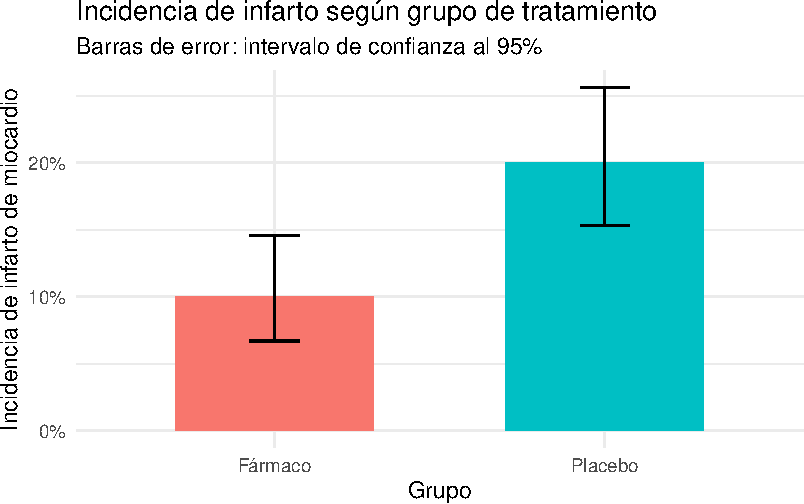
\includegraphics[keepaspectratio]{07-estudios-experimentales_files/figure-pdf/unnamed-chunk-5-1.pdf}}

El gráfico muestra que la incidencia observada en el grupo tratado con
el fármaco es claramente inferior a la del grupo placebo, aunque los
intervalos de confianza recuerdan que ambas incidencias se han estimado
a partir de una muestra y están sujetas a variabilidad muestral.

\subsection{Cálculo del tamaño
muestral}\label{cuxe1lculo-del-tamauxf1o-muestral}

Antes de iniciar un ensayo clínico es necesario determinar cuántos
pacientes por grupo se van a reclutar, de forma que el estudio tenga
potencia suficiente para detectar la diferencia de incidencias que se
considera clínicamente relevante, si esta existe realmente. El paquete
\texttt{pwr} permite realizar este cálculo para la comparación de dos
proporciones con la función \texttt{pwr.2p.test()}, que requiere el
tamaño del efecto de Cohen \texttt{h} (calculado a partir de las dos
proporciones con \texttt{ES.h()}), el nivel de significación
\texttt{sig.level} y la potencia deseada \texttt{power}.

Supóngase que, antes de realizar el ensayo del ejemplo anterior, se
quiere diseñar un estudio capaz de detectar una reducción de la
incidencia de infarto del 20\% (grupo control) al 10\% (grupo
experimental), con una potencia del 80\% y un nivel de significación del
5\%:

\begin{Shaded}
\begin{Highlighting}[]
\NormalTok{tamano\_efecto }\OtherTok{\textless{}{-}} \FunctionTok{ES.h}\NormalTok{(}\AttributeTok{p1 =} \FloatTok{0.10}\NormalTok{, }\AttributeTok{p2 =} \FloatTok{0.20}\NormalTok{)}
\NormalTok{tamano\_efecto}
\end{Highlighting}
\end{Shaded}

\begin{verbatim}
[1] -0.2837941
\end{verbatim}

\begin{Shaded}
\begin{Highlighting}[]
\NormalTok{calculo\_muestra }\OtherTok{\textless{}{-}} \FunctionTok{pwr.2p.test}\NormalTok{(}\AttributeTok{h =}\NormalTok{ tamano\_efecto, }\AttributeTok{sig.level =} \FloatTok{0.05}\NormalTok{, }\AttributeTok{power =} \FloatTok{0.8}\NormalTok{)}
\NormalTok{calculo\_muestra}
\end{Highlighting}
\end{Shaded}

\begin{verbatim}

     Difference of proportion power calculation for binomial distribution (arcsine transformation) 

              h = 0.2837941
              n = 194.9081
      sig.level = 0.05
          power = 0.8
    alternative = two.sided

NOTE: same sample sizes
\end{verbatim}

\begin{Shaded}
\begin{Highlighting}[]
\NormalTok{n\_por\_grupo }\OtherTok{\textless{}{-}} \FunctionTok{ceiling}\NormalTok{(calculo\_muestra}\SpecialCharTok{$}\NormalTok{n)}
\NormalTok{n\_por\_grupo}
\end{Highlighting}
\end{Shaded}

\begin{verbatim}
[1] 195
\end{verbatim}

El resultado indica que serían necesarios aproximadamente 195 pacientes
por grupo (es decir, un total de 390 pacientes) para tener una
probabilidad del 80\% de detectar, con un nivel de significación del
5\%, una diferencia de incidencias como la observada en el ejemplo si
esta existe realmente en la población. Con los 250 pacientes por grupo
reclutados en el ejemplo anterior, el estudio contaba con potencia más
que suficiente para detectar una diferencia de esa magnitud; en la
práctica, este cálculo debe realizarse siempre antes de iniciar el
reclutamiento, y no a posteriori, para justificar el tamaño de la
muestra planificada.

\section{Cuándo utilizar este
diseño}\label{cuuxe1ndo-utilizar-este-diseuxf1o-5}

El ensayo clínico aleatorizado es el diseño de elección siempre que sea
factible desde el punto de vista ético y práctico llevarlo a cabo, ya
que ofrece la evidencia más sólida para establecer que una exposición o
tratamiento causa un determinado resultado. Resulta especialmente
indicado en las fases de evaluación de nuevos fármacos, vacunas o
intervenciones sanitarias, antes de su aprobación y uso generalizado.
Sin embargo, cuando no es posible asignar aleatoriamente la exposición,
bien porque sería contrario a la ética (por ejemplo, asignar el consumo
de tabaco), bien por motivos prácticos, de coste o de tiempo, es
necesario recurrir a un
\href{08-estudios-cuasiexperimentales.qmd}{estudio cuasiexperimental},
que conserva la intervención activa del investigador pero renuncia a la
aleatorización, o bien a alguno de los diseños observacionales
estudiados en los capítulos anteriores.

\chapter{Estudios
cuasiexperimentales}\label{estudios-cuasiexperimentales}

Un \textbf{estudio cuasiexperimental} es un tipo de estudio en el que el
investigador interviene, es decir, aplica un tratamiento, programa o
intervención a los individuos, pero \textbf{sin asignar aleatoriamente}
a los sujetos a los grupos de tratamiento y de control. Esta ausencia de
aleatorización es la característica que lo distingue de los
\hyperref[estudios-experimentales]{estudios experimentales}, tal y como
se introdujo en el
\hyperref[introducciuxf3n-a-los-tipos-de-estudios-estaduxedsticos]{capítulo
de introducción}.

Los estudios cuasiexperimentales surgen habitualmente cuando la
aleatorización no es posible, no es ética o no es práctica. Es el caso,
por ejemplo, de la evaluación de políticas públicas, programas
educativos o intervenciones comunitarias, en los que no se puede asignar
al azar qué municipios, colegios o pacientes reciben la intervención y
cuáles no, ya sea por razones logísticas, legales o de justicia social.

\section{Definición y
características}\label{definiciuxf3n-y-caracteruxedsticas-6}

En un estudio cuasiexperimental el investigador manipula deliberadamente
una variable independiente (la intervención o tratamiento) y mide su
efecto sobre una o varias variables dependientes, pero los grupos que
reciben o no la intervención se forman por procedimientos distintos del
azar: por ejemplo, porque ya existían previamente (dos colegios, dos
regiones), porque los propios individuos se autoseleccionan, o porque la
intervención se aplica a toda una comunidad sin grupo de comparación
disponible.

Existen numerosas variantes de diseño cuasiexperimental, entre las que
destacan las tres siguientes.

\subsection{Diseño de un solo grupo
antes-después}\label{diseuxf1o-de-un-solo-grupo-antes-despuuxe9s}

También llamado diseño \emph{one-group pretest-posttest}, consiste en
medir una variable de interés en un único grupo de individuos antes de
aplicar la intervención y volver a medirla después. Es el diseño
cuasiexperimental más sencillo, ya que no requiere ningún grupo de
comparación, pero también el más débil desde el punto de vista de la
validez interna, porque cualquier cambio observado entre el antes y el
después podría deberse a la intervención, pero también a otros factores
que hayan actuado simultáneamente sobre los individuos.

\subsection{Diseño con grupo de control no
equivalente}\label{diseuxf1o-con-grupo-de-control-no-equivalente}

En este diseño se dispone de dos grupos, uno que recibe la intervención
(grupo tratado) y otro que no la recibe (grupo de control o de
comparación), y se mide la variable de interés en ambos antes y después
de la intervención. La diferencia esencial respecto a un experimento es
que los dos grupos no se han formado mediante asignación aleatoria, sino
que ya existían como tales (dos aulas, dos hospitales, dos regiones),
por lo que pueden diferir sistemáticamente en características que
también influyan en el resultado. Es el diseño cuasiexperimental más
utilizado en la práctica y el que permite construir el estimador de
diferencia en diferencias que se presenta más adelante.

\subsection{Series temporales
interrumpidas}\label{series-temporales-interrumpidas}

En este diseño se realizan múltiples mediciones de la variable de
interés sobre la misma unidad de estudio (una población, una región, una
organización) tanto antes como después de que se produzca la
intervención, que actúa como una interrupción en la serie temporal. Por
ejemplo, registrar la tasa de accidentes de tráfico mes a mes durante
varios años antes y después de la entrada en vigor de una nueva ley de
seguridad vial. La disponibilidad de varias medidas antes y después, en
lugar de una sola, permite valorar si el cambio observado tras la
intervención rompe con la tendencia previa o si es simplemente una
continuación de una tendencia ya existente.

\section{Ventajas e inconvenientes}\label{ventajas-e-inconvenientes-6}

Los estudios cuasiexperimentales presentan las siguientes ventajas:

\begin{itemize}
\tightlist
\item
  Son más factibles, tanto éticamente como en la práctica, que un ensayo
  controlado aleatorizado, ya que no requieren asignar al azar a los
  individuos a recibir o no una intervención.
\item
  Permiten evaluar intervenciones a gran escala, como políticas
  públicas, leyes o programas comunitarios, que no podrían implementarse
  de forma aleatorizada.
\item
  Suelen ser más baratos y rápidos de llevar a cabo que un experimento,
  al aprovechar grupos o mediciones ya existentes.
\end{itemize}

Y también los siguientes inconvenientes:

\begin{itemize}
\tightlist
\item
  Al no existir aleatorización, existe un mayor riesgo de \textbf{sesgo
  de selección}: los grupos comparados pueden diferir sistemáticamente
  en características relevantes, y no solo en si reciben o no la
  intervención.
\item
  Es más difícil descartar la presencia de \textbf{factores de
  confusión} que expliquen, total o parcialmente, el cambio observado.
\item
  Están expuestos a amenazas a la validez interna propias de los diseños
  con medidas repetidas, como la \textbf{regresión a la media} (los
  valores extremos tienden a acercarse a la media en mediciones
  sucesivas, con independencia de la intervención) o la
  \textbf{historia} (sucesos externos a la intervención, ocurridos entre
  el antes y el después, que también podrían explicar el cambio).
\end{itemize}

\section{Medidas propias de este
diseño}\label{medidas-propias-de-este-diseuxf1o-6}

En el diseño con grupo de control no equivalente, la medida de efecto
más habitual es el estimador de \textbf{diferencia en diferencias}.

\begin{definition}[Diferencia en diferencias
(DiD)]\protect\hypertarget{def-cuasiexperimentales-diferencia-en-diferencias}{}\label{def-cuasiexperimentales-diferencia-en-diferencias}

Dado un grupo tratado y un grupo de control no equivalente, en los que
se mide una variable de interés antes y después de aplicar una
intervención sobre el grupo tratado, siendo \(\bar{Y}_{t,antes}\) y
\(\bar{Y}_{t,despues}\) las medias de la variable en el grupo tratado
antes y después de la intervención, y \(\bar{Y}_{c,antes}\) y
\(\bar{Y}_{c,despues}\) las medias correspondientes en el grupo de
control, se define el estimador de diferencia en diferencias como

\[DiD = (\bar{Y}_{t,despues} - \bar{Y}_{t,antes}) - (\bar{Y}_{c,despues} - \bar{Y}_{c,antes})\]

\end{definition}

\begin{tcolorbox}[enhanced jigsaw, arc=.35mm, bottomrule=.15mm, bottomtitle=1mm, breakable, colback=white, colbacktitle=quarto-callout-note-color!10!white, colframe=quarto-callout-note-color-frame, coltitle=black, left=2mm, leftrule=.75mm, opacityback=0, opacitybacktitle=0.6, rightrule=.15mm, title=\textcolor{quarto-callout-note-color}{\faInfo}\hspace{0.5em}{Interpretación}, titlerule=0mm, toprule=.15mm, toptitle=1mm]

El estimador \(DiD\) representa el efecto atribuible a la intervención
una vez descontado el cambio que se habría producido de todos modos, sin
necesidad de intervenir. El cambio observado en el grupo de control se
utiliza como estimación de la \textbf{tendencia contrafactual}, es
decir, de lo que habría ocurrido en el grupo tratado si no hubiera
recibido la intervención. Restar ese cambio al cambio observado en el
grupo tratado permite aislar el efecto propio de la intervención.

\end{tcolorbox}

\begin{tcolorbox}[enhanced jigsaw, arc=.35mm, bottomrule=.15mm, bottomtitle=1mm, breakable, colback=white, colbacktitle=quarto-callout-warning-color!10!white, colframe=quarto-callout-warning-color-frame, coltitle=black, left=2mm, leftrule=.75mm, opacityback=0, opacitybacktitle=0.6, rightrule=.15mm, title=\textcolor{quarto-callout-warning-color}{\faExclamationTriangle}\hspace{0.5em}{Advertencia}, titlerule=0mm, toprule=.15mm, toptitle=1mm]

El estimador de diferencia en diferencias solo es válido bajo el
\textbf{supuesto de tendencias paralelas}: en ausencia de la
intervención, el grupo tratado y el grupo de control habrían
evolucionado de forma paralela, es decir, con el mismo cambio medio
entre el antes y el después. Si este supuesto no se cumple, la \(DiD\)
puede sobrestimar o infraestimar el verdadero efecto de la intervención.

\end{tcolorbox}

\begin{example}[]\protect\hypertarget{exm-cuasiexperimentales-did-refuerzo-escolar}{}\label{exm-cuasiexperimentales-did-refuerzo-escolar}

Un ayuntamiento implanta un programa de refuerzo escolar en los colegios
de su municipio (grupo tratado). Para valorar su efecto, se compara la
calificación media de los alumnos en una prueba estandarizada con la de
los colegios de un municipio vecino que no recibió el programa (grupo de
control), antes y después de su implantación. No es posible asignar
aleatoriamente qué municipio recibe el programa, por lo que se trata de
un diseño cuasiexperimental con grupo de control no equivalente.

Las calificaciones medias obtenidas son

\[
\begin{array}{lrrr}
\hline
\mbox{Grupo} & \mbox{Antes} & \mbox{Después} & \mbox{Cambio}\\
\hline
\mbox{Tratado (con programa)} & 5.2 & 6.4 & 1.2\\
\mbox{Control (sin programa)} & 5.3 & 5.6 & 0.3\\
\hline
\end{array}
\]

El cambio en el grupo tratado es

\[\bar{Y}_{t,despues} - \bar{Y}_{t,antes} = 6.4 - 5.2 = 1.2,\]

y el cambio en el grupo de control, que estima la tendencia que habría
seguido el grupo tratado sin el programa, es

\[\bar{Y}_{c,despues} - \bar{Y}_{c,antes} = 5.6 - 5.3 = 0.3.\]

Por tanto, el estimador de diferencia en diferencias es

\[DiD = 1.2 - 0.3 = 0.9.\]

Descontada la tendencia común a ambos municipios, el programa de
refuerzo escolar habría producido un aumento medio de 0.9 puntos en la
calificación de los alumnos.

\end{example}

\section{Realización con R}\label{realizaciuxf3n-con-r-6}

\subsection{Cálculo de la diferencia en
diferencias}\label{cuxe1lculo-de-la-diferencia-en-diferencias}

A continuación se reproduce en R el cálculo del ejemplo anterior a
partir de las cuatro medias observadas.

\begin{Shaded}
\begin{Highlighting}[]
\NormalTok{y\_t\_antes }\OtherTok{\textless{}{-}} \FloatTok{5.2}
\NormalTok{y\_t\_despues }\OtherTok{\textless{}{-}} \FloatTok{6.4}
\NormalTok{y\_c\_antes }\OtherTok{\textless{}{-}} \FloatTok{5.3}
\NormalTok{y\_c\_despues }\OtherTok{\textless{}{-}} \FloatTok{5.6}

\NormalTok{cambio\_tratado }\OtherTok{\textless{}{-}}\NormalTok{ y\_t\_despues }\SpecialCharTok{{-}}\NormalTok{ y\_t\_antes}
\NormalTok{cambio\_control }\OtherTok{\textless{}{-}}\NormalTok{ y\_c\_despues }\SpecialCharTok{{-}}\NormalTok{ y\_c\_antes}
\NormalTok{DiD }\OtherTok{\textless{}{-}}\NormalTok{ cambio\_tratado }\SpecialCharTok{{-}}\NormalTok{ cambio\_control}

\NormalTok{cambio\_tratado}
\end{Highlighting}
\end{Shaded}

\begin{verbatim}
[1] 1.2
\end{verbatim}

\begin{Shaded}
\begin{Highlighting}[]
\NormalTok{cambio\_control}
\end{Highlighting}
\end{Shaded}

\begin{verbatim}
[1] 0.3
\end{verbatim}

\begin{Shaded}
\begin{Highlighting}[]
\NormalTok{DiD}
\end{Highlighting}
\end{Shaded}

\begin{verbatim}
[1] 0.9
\end{verbatim}

El resultado coincide con el obtenido a mano: un cambio de 1.2 puntos en
el grupo tratado, un cambio de 0.3 puntos en el grupo de control, y una
diferencia en diferencias de 0.9 puntos.

El gráfico clásico de diferencia en diferencias representa, para cada
grupo, la evolución de la media entre el antes y el después mediante una
línea. La divergencia entre ambas líneas tras la intervención es
visualmente atribuible al efecto del programa.

\begin{Shaded}
\begin{Highlighting}[]
\NormalTok{datos\_did }\OtherTok{\textless{}{-}} \FunctionTok{tibble}\NormalTok{(}
  \AttributeTok{grupo =} \FunctionTok{rep}\NormalTok{(}\FunctionTok{c}\NormalTok{(}\StringTok{"Tratado"}\NormalTok{, }\StringTok{"Control"}\NormalTok{), }\AttributeTok{each =} \DecValTok{2}\NormalTok{),}
  \AttributeTok{momento =} \FunctionTok{rep}\NormalTok{(}\FunctionTok{c}\NormalTok{(}\StringTok{"Antes"}\NormalTok{, }\StringTok{"Después"}\NormalTok{), }\AttributeTok{times =} \DecValTok{2}\NormalTok{),}
  \AttributeTok{media =} \FunctionTok{c}\NormalTok{(y\_t\_antes, y\_t\_despues, y\_c\_antes, y\_c\_despues)}
\NormalTok{) }\SpecialCharTok{|\textgreater{}}
  \FunctionTok{mutate}\NormalTok{(}\AttributeTok{momento =} \FunctionTok{factor}\NormalTok{(momento, }\AttributeTok{levels =} \FunctionTok{c}\NormalTok{(}\StringTok{"Antes"}\NormalTok{, }\StringTok{"Después"}\NormalTok{)))}

\FunctionTok{ggplot}\NormalTok{(datos\_did, }\FunctionTok{aes}\NormalTok{(}\AttributeTok{x =}\NormalTok{ momento, }\AttributeTok{y =}\NormalTok{ media, }\AttributeTok{group =}\NormalTok{ grupo, }\AttributeTok{color =}\NormalTok{ grupo)) }\SpecialCharTok{+}
  \FunctionTok{geom\_line}\NormalTok{(}\AttributeTok{linewidth =} \DecValTok{1}\NormalTok{) }\SpecialCharTok{+}
  \FunctionTok{geom\_point}\NormalTok{(}\AttributeTok{size =} \DecValTok{3}\NormalTok{) }\SpecialCharTok{+}
  \FunctionTok{labs}\NormalTok{(}
    \AttributeTok{x =} \StringTok{"Momento"}\NormalTok{,}
    \AttributeTok{y =} \StringTok{"Calificación media"}\NormalTok{,}
    \AttributeTok{color =} \StringTok{"Grupo"}\NormalTok{,}
    \AttributeTok{title =} \StringTok{"Diferencia en diferencias del programa de refuerzo escolar"}
\NormalTok{  ) }\SpecialCharTok{+}
  \FunctionTok{theme\_minimal}\NormalTok{()}
\end{Highlighting}
\end{Shaded}

\pandocbounded{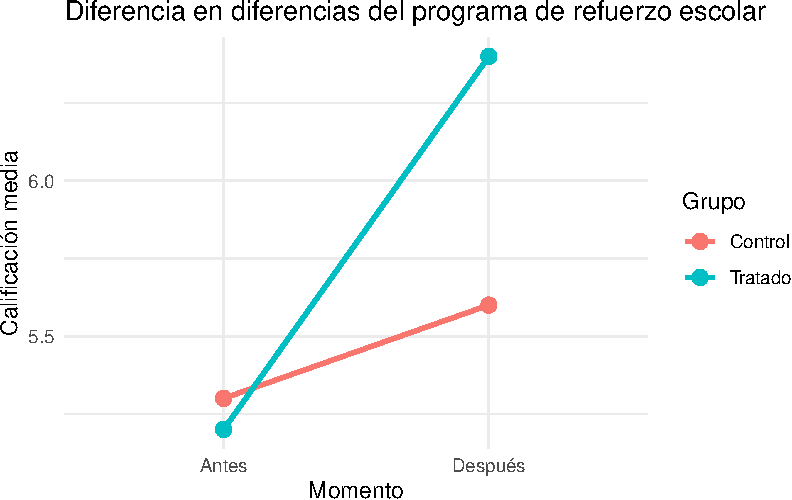
\includegraphics[keepaspectratio]{08-estudios-cuasiexperimentales_files/figure-pdf/unnamed-chunk-2-1.pdf}}

En el gráfico se aprecia que, aunque ambos grupos mejoran ligeramente
entre el antes y el después, el grupo tratado lo hace en mayor medida
que el grupo de control, y esa distancia adicional es precisamente la
\(DiD\) calculada.

\subsection{Diseño de un solo grupo
antes-después}\label{diseuxf1o-de-un-solo-grupo-antes-despuuxe9s-1}

Cuando no se dispone de ningún grupo de control, el diseño más simple
consiste en comparar las mediciones de los mismos individuos antes y
después de la intervención mediante un contraste de datos pareados. A
continuación se simula una muestra de 30 individuos a los que se aplica
una intervención (por ejemplo, un programa de entrenamiento cognitivo) y
se mide su rendimiento antes y después.

\begin{Shaded}
\begin{Highlighting}[]
\FunctionTok{set.seed}\NormalTok{(}\DecValTok{123}\NormalTok{)}
\NormalTok{n }\OtherTok{\textless{}{-}} \DecValTok{30}
\NormalTok{antes }\OtherTok{\textless{}{-}} \FunctionTok{rnorm}\NormalTok{(n, }\AttributeTok{mean =} \DecValTok{50}\NormalTok{, }\AttributeTok{sd =} \DecValTok{8}\NormalTok{)}
\NormalTok{despues }\OtherTok{\textless{}{-}}\NormalTok{ antes }\SpecialCharTok{+} \FunctionTok{rnorm}\NormalTok{(n, }\AttributeTok{mean =} \DecValTok{4}\NormalTok{, }\AttributeTok{sd =} \DecValTok{5}\NormalTok{)}

\NormalTok{datos\_pretest\_postest }\OtherTok{\textless{}{-}} \FunctionTok{tibble}\NormalTok{(}
  \AttributeTok{individuo =} \DecValTok{1}\SpecialCharTok{:}\NormalTok{n,}
  \AttributeTok{antes =}\NormalTok{ antes,}
  \AttributeTok{despues =}\NormalTok{ despues}
\NormalTok{)}

\NormalTok{datos\_pretest\_postest}
\end{Highlighting}
\end{Shaded}

\begin{verbatim}
# A tibble: 30 x 3
   individuo antes despues
       <int> <dbl>   <dbl>
 1         1  45.5    51.6
 2         2  48.2    50.7
 3         3  62.5    70.9
 4         4  50.6    59.0
 5         5  51.0    59.1
 6         6  63.7    71.2
 7         7  53.7    60.5
 8         8  39.9    43.6
 9         9  44.5    47.0
10        10  46.4    48.5
# i 20 more rows
\end{verbatim}

Para contrastar si el cambio medio observado es estadísticamente
significativo se aplica un contraste \(t\) de Student para datos
pareados:

\begin{Shaded}
\begin{Highlighting}[]
\FunctionTok{t.test}\NormalTok{(datos\_pretest\_postest}\SpecialCharTok{$}\NormalTok{despues, datos\_pretest\_postest}\SpecialCharTok{$}\NormalTok{antes, }\AttributeTok{paired =} \ConstantTok{TRUE}\NormalTok{)}
\end{Highlighting}
\end{Shaded}

\begin{verbatim}

    Paired t-test

data:  datos_pretest_postest$despues and datos_pretest_postest$antes
t = 6.4165, df = 29, p-value = 5.115e-07
alternative hypothesis: true mean difference is not equal to 0
95 percent confidence interval:
 3.332482 6.450901
sample estimates:
mean difference 
       4.891692 
\end{verbatim}

El p-valor obtenido es prácticamente cero, muy inferior a 0.05, por lo
que se rechaza la hipótesis nula de que no existe cambio medio entre el
antes y el después: el rendimiento medio tras la intervención es
significativamente superior al previo. Sin embargo, al tratarse de un
diseño de un solo grupo, este resultado no permite descartar que el
cambio se deba a otros factores distintos de la intervención (maduración
de los individuos, práctica en la propia prueba, sucesos externos
ocurridos durante el estudio, etc.), que es precisamente la principal
limitación de este diseño frente al que incorpora un grupo de control no
equivalente.

\section{Cuándo utilizar este
diseño}\label{cuuxe1ndo-utilizar-este-diseuxf1o-6}

Un estudio cuasiexperimental es la opción adecuada cuando el
investigador puede intervenir aplicando un tratamiento o programa, pero
no puede asignar aleatoriamente a los individuos o unidades a los grupos
de tratamiento y control, como ocurre con frecuencia en la evaluación de
políticas públicas, programas educativos o intervenciones comunitarias.
Se diferencia así de los \hyperref[estudios-experimentales]{estudios
experimentales}, que deben preferirse siempre que la aleatorización sea
posible y ética, ya que ofrecen un control mucho mayor sobre los
factores de confusión. Y se diferencia de los
\hyperref[estudios-de-cohortes]{estudios de cohortes} en que en estos
últimos el investigador no interviene en absoluto, limitándose a
observar y seguir en el tiempo a individuos que ya están expuestos o no
a un factor por decisión propia o por las circunstancias, sin aplicar
ningún tratamiento. En definitiva, el diseño cuasiexperimental ocupa un
lugar intermedio entre la observación pura y el experimento controlado,
y resulta especialmente útil cuando la pregunta de investigación exige
valorar el efecto de una intervención real que no puede aleatorizarse.

\chapter{Encuestas y diseño de
muestreo}\label{encuestas-y-diseuxf1o-de-muestreo}

Como se adelantó en el
\hyperref[introducciuxf3n-a-los-tipos-de-estudios-estaduxedsticos]{capítulo
de introducción}, la encuesta es probablemente el instrumento de
recogida de datos más extendido en estadística aplicada: consiste en
seleccionar una muestra de individuos de una población y medir sobre
ellos, mediante un cuestionario u otro procedimiento de observación, una
o varias variables de interés (opiniones, hábitos, características
sociodemográficas, intención de voto, etc.). En la mayoría de los casos
comparte con el \hyperref[estudios-transversales]{estudio transversal}
la misma lógica temporal, ya que las variables se registran en un único
momento, sobre una muestra tomada de la población general sin
condicionar la selección a ninguna exposición o resultado previo. Sin
embargo, mientras que en los capítulos anteriores el foco estaba en el
tipo de diseño observacional o experimental, en este capítulo el foco se
traslada a una cuestión transversal a todos ellos y crítica para la
validez de cualquier estudio: \textbf{cómo se selecciona la muestra} a
partir de la cual se pretende estimar o inferir características de toda
la población.

\section{Definición y
características}\label{definiciuxf3n-y-caracteruxedsticas-7}

\begin{definition}[Encuesta
estadística]\protect\hypertarget{def-encuestas-encuesta-estadistica}{}\label{def-encuestas-encuesta-estadistica}

Una \emph{encuesta estadística} es un procedimiento de investigación que
consiste en seleccionar una muestra de individuos de una población,
mediante un método de muestreo determinado, y recoger información sobre
ellos (habitualmente a través de un cuestionario) con el fin de estimar
características, opiniones o comportamientos de la población de la que
proceden.

\end{definition}

La validez de las conclusiones de una encuesta depende, en gran medida,
de que la muestra seleccionada sea representativa de la población
objetivo. Esto exige, en primer lugar, disponer de un marco muestral
adecuado.

\begin{definition}[Marco
muestral]\protect\hypertarget{def-encuestas-marco-muestral}{}\label{def-encuestas-marco-muestral}

El \emph{marco muestral} (en inglés, \emph{sampling frame}) es el
listado, registro o procedimiento que permite identificar y acceder a
todos los elementos de la población objetivo, de manera que cada uno de
ellos pueda ser seleccionado para formar parte de la muestra.

\end{definition}

Un marco muestral incompleto o desactualizado (por ejemplo, un censo de
población antiguo, o un listado telefónico que excluye a quienes solo
disponen de móvil) introduce un sesgo de cobertura, ya que ciertos
segmentos de la población tienen probabilidad nula o muy baja de ser
seleccionados, con independencia de lo riguroso que sea el método de
muestreo empleado posteriormente.

Cuando se dispone de un marco muestral adecuado, existen varios diseños
de \textbf{muestreo probabilístico}, en los que cada elemento de la
población tiene una probabilidad conocida (y no nula) de ser
seleccionado, lo que permite calcular la precisión de las estimaciones y
generalizarlas a la población con garantías estadísticas. Los
principales son los siguientes.

\subsection{Muestreo aleatorio simple
(MAS)}\label{muestreo-aleatorio-simple-mas}

En el \emph{muestreo aleatorio simple} cada elemento de la población
tiene la misma probabilidad de ser seleccionado, y la selección de cada
individuo es independiente de la de los demás. Es el diseño de
referencia, el más sencillo de analizar, pero exige disponer de un marco
muestral completo y puede resultar poco eficiente cuando la población es
muy heterogénea o está muy dispersa geográficamente.

\subsection{Muestreo estratificado}\label{muestreo-estratificado}

En el \emph{muestreo estratificado} la población se divide previamente
en subgrupos o \textbf{estratos}, internamente lo más homogéneos posible
respecto a la variable de interés y heterogéneos entre sí (por ejemplo,
comunidades autónomas, tramos de edad o tipo de centro educativo), y
dentro de cada estrato se selecciona una muestra aleatoria simple de
manera independiente. Cuando el tamaño de la muestra en cada estrato se
reparte en proporción al peso de dicho estrato en la población, se habla
de \textbf{afijación proporcional}. Al garantizar la presencia de todos
los estratos en la proporción adecuada, este diseño suele producir
estimaciones más precisas que el muestreo aleatorio simple, para un
mismo tamaño de muestra, siempre que los estratos sean realmente
homogéneos internamente.

\subsection{Muestreo por
conglomerados}\label{muestreo-por-conglomerados}

En el \emph{muestreo por conglomerados} (o \emph{por clusters}) la
población se divide en grupos naturales o preexistentes (conglomerados),
como colegios, manzanas de una ciudad o centros de salud, y en lugar de
seleccionar individuos se seleccionan aleatoriamente algunos
conglomerados completos, incluyendo a todos sus miembros en la muestra
(o, en su versión bietápica, seleccionando después una submuestra dentro
de cada conglomerado elegido). Resulta especialmente útil cuando no
existe un marco muestral de individuos pero sí de conglomerados, y
reduce mucho el coste logístico al concentrar el trabajo de campo en
unas pocas zonas. A cambio, suele perder precisión respecto al muestreo
aleatorio simple, ya que los individuos de un mismo conglomerado tienden
a parecerse entre sí.

\subsection{Muestreo sistemático}\label{muestreo-sistemuxe1tico}

En el \emph{muestreo sistemático} se ordena el marco muestral (por
ejemplo, un listado de \(N\) individuos), se calcula un intervalo de
selección \(k = N/n\) (siendo \(n\) el tamaño de muestra deseado), se
elige aleatoriamente un punto de partida entre \(1\) y \(k\), y a partir
de él se selecciona cada \(k\)-ésimo elemento de la lista. Es fácil de
aplicar y, cuando el listado no sigue ningún patrón periódico
relacionado con la variable de interés, suele proporcionar resultados
muy similares a los del muestreo aleatorio simple.

Además de estos diseños probabilísticos, existen métodos de
\textbf{muestreo no probabilístico}, como el muestreo por conveniencia
(se selecciona a los individuos más accesibles) o el muestreo en bola de
nieve (los participantes reclutan a su vez a otros participantes). Estos
métodos son más rápidos y baratos, pero al no conocerse la probabilidad
de selección de cada individuo no permiten calcular la precisión de las
estimaciones ni generalizar los resultados a la población con garantías
estadísticas, por lo que su uso queda habitualmente restringido a
estudios exploratorios o poblaciones muy difíciles de acceder.

\section{Ventajas e inconvenientes}\label{ventajas-e-inconvenientes-7}

\begin{itemize}
\tightlist
\item
  \textbf{Muestreo aleatorio simple}: es el más sencillo de diseñar y
  analizar, pero exige un marco muestral completo de individuos y puede
  resultar poco eficiente (mayor error para el mismo tamaño de muestra)
  cuando la población es heterogénea.
\item
  \textbf{Muestreo estratificado}: mejora la precisión frente al
  muestreo aleatorio simple cuando existen variables (estratos)
  fuertemente relacionadas con la variable de interés, y garantiza
  representación de todos los grupos relevantes; a cambio, requiere
  conocer de antemano el valor de la variable de estratificación para
  toda la población, lo que no siempre es posible.
\item
  \textbf{Muestreo por conglomerados}: es el más económico y
  logísticamente viable cuando la población está muy dispersa o no
  existe un marco muestral de individuos, pero suele ser el menos
  preciso, ya que los elementos de un mismo conglomerado tienden a ser
  parecidos entre sí (baja variabilidad interna, alta variabilidad entre
  conglomerados).
\item
  \textbf{Muestreo sistemático}: es muy fácil de implementar sobre un
  listado ordenado y suele comportarse como el muestreo aleatorio
  simple, pero puede introducir sesgos graves si el listado presenta
  algún patrón periódico que coincida con el intervalo de selección
  \(k\).
\item
  \textbf{Muestreo no probabilístico}: es el más rápido y barato, y en
  ocasiones la única opción viable (por ejemplo, para poblaciones
  ocultas o de difícil acceso), pero no permite cuantificar el error de
  muestreo ni generalizar los resultados a la población con garantías
  estadísticas.
\end{itemize}

\section{Medidas propias de este
diseño}\label{medidas-propias-de-este-diseuxf1o-7}

Además de las medidas descriptivas habituales (proporciones, medias,
etc.), calculadas ahora ponderando por el diseño muestral empleado, dos
cantidades son especialmente características del diseño de encuestas: el
error de muestreo de una estimación y el tamaño muestral necesario para
lograr una precisión determinada.

\subsection{Error de muestreo}\label{error-de-muestreo}

\begin{definition}[Error de
muestreo]\protect\hypertarget{def-encuestas-error-muestreo}{}\label{def-encuestas-error-muestreo}

Dada una muestra aleatoria simple de tamaño \(n\) en la que se ha
observado una proporción muestral \(\hat p\) de individuos que presentan
una determinada característica, el \emph{error de muestreo} (o margen de
error) de \(\hat p\) para un nivel de confianza \(1-\alpha\) se define
como

\[e = z_{\alpha/2}\sqrt{\frac{\hat p(1-\hat p)}{n}}\]

donde \(z_{\alpha/2}\) es el valor crítico de la distribución normal
estándar que deja una probabilidad \(\alpha/2\) a su derecha.

\end{definition}

\begin{tcolorbox}[enhanced jigsaw, arc=.35mm, bottomrule=.15mm, bottomtitle=1mm, breakable, colback=white, colbacktitle=quarto-callout-important-color!10!white, colframe=quarto-callout-important-color-frame, coltitle=black, left=2mm, leftrule=.75mm, opacityback=0, opacitybacktitle=0.6, rightrule=.15mm, title=\textcolor{quarto-callout-important-color}{\faExclamation}\hspace{0.5em}{Importante}, titlerule=0mm, toprule=.15mm, toptitle=1mm]

El error de muestreo es siempre un número no negativo,

\[e \geq 0,\]

y disminuye a medida que aumenta el tamaño de muestra \(n\),
concretamente en proporción a \(1/\sqrt{n}\): para reducir el error a la
mitad es necesario cuadruplicar el tamaño de muestra.

\end{tcolorbox}

\begin{tcolorbox}[enhanced jigsaw, arc=.35mm, bottomrule=.15mm, bottomtitle=1mm, breakable, colback=white, colbacktitle=quarto-callout-note-color!10!white, colframe=quarto-callout-note-color-frame, coltitle=black, left=2mm, leftrule=.75mm, opacityback=0, opacitybacktitle=0.6, rightrule=.15mm, title=\textcolor{quarto-callout-note-color}{\faInfo}\hspace{0.5em}{Interpretación}, titlerule=0mm, toprule=.15mm, toptitle=1mm]

\begin{itemize}
\tightlist
\item
  El error de muestreo cuantifica cuánto puede diferir, con la confianza
  especificada, la proporción muestral \(\hat p\) de la verdadera
  proporción poblacional \(p\), exclusivamente por el hecho de trabajar
  con una muestra y no con toda la población.
\item
  El intervalo \((\hat p - e,\ \hat p + e)\) es precisamente el
  intervalo de confianza al nivel \(1-\alpha\) para la proporción
  poblacional \(p\).
\item
  El error de muestreo no recoge otras fuentes de error ajenas al azar,
  como el sesgo de no respuesta, el sesgo de cobertura del marco
  muestral o los errores de medición del cuestionario, que pueden ser
  tanto o más importantes que el propio error de muestreo.
\end{itemize}

\end{tcolorbox}

\subsection{Tamaño muestral
necesario}\label{tamauxf1o-muestral-necesario}

En la práctica, la pregunta habitual no es ``¿qué error tiene mi
muestra?'' sino la inversa: ``¿qué tamaño de muestra necesito para que
el error no supere un determinado valor?''. Despejando \(n\) de la
fórmula del error de muestreo se obtiene la siguiente expresión.

\begin{definition}[Tamaño muestral
necesario]\protect\hypertarget{def-encuestas-tamano-muestral}{}\label{def-encuestas-tamano-muestral}

Para estimar una proporción poblacional \(p\) con un error de muestreo
máximo \(e\) y un nivel de confianza \(1-\alpha\), el tamaño de muestra
necesario, suponiendo muestreo aleatorio simple sobre una población de
tamaño muy superior a la muestra, es

\[n = \frac{z_{\alpha/2}^2\, p(1-p)}{e^2}\]

donde \(p\) es un valor aproximado (de un estudio previo o piloto) de la
proporción que se quiere estimar; si no se dispone de tal valor, se toma
\(p=0.5\), ya que es el valor que maximiza \(p(1-p)\) y por tanto
produce el tamaño de muestra más conservador (el mayor posible).

\end{definition}

\begin{tcolorbox}[enhanced jigsaw, arc=.35mm, bottomrule=.15mm, bottomtitle=1mm, breakable, colback=white, colbacktitle=quarto-callout-important-color!10!white, colframe=quarto-callout-important-color-frame, coltitle=black, left=2mm, leftrule=.75mm, opacityback=0, opacitybacktitle=0.6, rightrule=.15mm, title=\textcolor{quarto-callout-important-color}{\faExclamation}\hspace{0.5em}{Importante}, titlerule=0mm, toprule=.15mm, toptitle=1mm]

Cuando la población tiene un tamaño finito y conocido \(N\) que no es
muy superior al tamaño de muestra calculado, puede aplicarse el
\emph{factor de corrección para poblaciones finitas},

\[n_{ajustado} = \frac{n}{1+\dfrac{n-1}{N}},\]

que reduce ligeramente el tamaño de muestra necesario. En la práctica,
cuando \(N\) es grande frente a \(n\) (por ejemplo, encuestas sobre la
población de un país o una ciudad grande), esta corrección apenas tiene
efecto y suele omitirse.

\end{tcolorbox}

\begin{tcolorbox}[enhanced jigsaw, arc=.35mm, bottomrule=.15mm, bottomtitle=1mm, breakable, colback=white, colbacktitle=quarto-callout-note-color!10!white, colframe=quarto-callout-note-color-frame, coltitle=black, left=2mm, leftrule=.75mm, opacityback=0, opacitybacktitle=0.6, rightrule=.15mm, title=\textcolor{quarto-callout-note-color}{\faInfo}\hspace{0.5em}{Interpretación}, titlerule=0mm, toprule=.15mm, toptitle=1mm]

\begin{itemize}
\tightlist
\item
  El tamaño muestral necesario aumenta con el nivel de confianza exigido
  (mayor \(z_{\alpha/2}\)) y disminuye rápidamente al relajar la
  precisión exigida (mayor \(e\)), ya que \(n\) depende del cuadrado de
  \(e\) en el denominador.
\item
  El tamaño muestral necesario es máximo cuando \(p=0.5\) y disminuye a
  medida que \(p\) se aleja de \(0.5\) hacia \(0\) o hacia \(1\), ya que
  fenómenos muy raros o muy comunes son, en cierto sentido, más fáciles
  de acotar con precisión.
\item
  Esta fórmula corresponde al muestreo aleatorio simple; en diseños
  estratificados, por conglomerados o sistemáticos, el tamaño necesario
  puede ser menor o mayor, en función de si el diseño mejora o empeora
  la precisión respecto al muestreo aleatorio simple.
\end{itemize}

\end{tcolorbox}

\begin{example}[]\protect\hypertarget{exm-encuestas-tamano-muestral}{}\label{exm-encuestas-tamano-muestral}

Se quiere diseñar una encuesta para estimar la proporción de la
población de una ciudad que está a favor de un determinado proyecto
urbanístico, con un error de muestreo máximo de \(e=0.03\) (tres puntos
porcentuales) y un nivel de confianza del \(95\%\) (\(\alpha=0.05\), por
lo que \(z_{\alpha/2}=1.96\)). Al no disponer de información previa
sobre la proporción real, se toma el valor más conservador, \(p=0.5\).
El tamaño de muestra necesario es

\[n = \frac{z_{\alpha/2}^2\, p(1-p)}{e^2} = \frac{1.96^2 \times 0.5 \times 0.5}{0.03^2} = \frac{0.9604}{0.0009} \approx 1067.1.\]

Redondeando hacia arriba, se necesitaría una muestra de \(n=1068\)
individuos para garantizar, con una confianza del \(95\%\), que la
proporción estimada no se aleje de la verdadera proporción poblacional
en más de tres puntos porcentuales.

\end{example}

\section{Realización con R}\label{realizaciuxf3n-con-r-7}

\subsection{Cálculo del tamaño muestral
necesario}\label{cuxe1lculo-del-tamauxf1o-muestral-necesario}

En primer lugar se reproduce en R el cálculo manual del
Ejemplo~\ref{exm-encuestas-tamano-muestral}, obteniendo el valor crítico
\(z_{\alpha/2}\) con \texttt{qnorm()} y aplicando directamente la
fórmula del tamaño muestral:

\begin{Shaded}
\begin{Highlighting}[]
\NormalTok{calcular\_n }\OtherTok{\textless{}{-}} \ControlFlowTok{function}\NormalTok{(e, }\AttributeTok{confianza =} \FloatTok{0.95}\NormalTok{, }\AttributeTok{p =} \FloatTok{0.5}\NormalTok{) \{}
\NormalTok{  alpha }\OtherTok{\textless{}{-}} \DecValTok{1} \SpecialCharTok{{-}}\NormalTok{ confianza}
\NormalTok{  z }\OtherTok{\textless{}{-}} \FunctionTok{qnorm}\NormalTok{(}\DecValTok{1} \SpecialCharTok{{-}}\NormalTok{ alpha }\SpecialCharTok{/} \DecValTok{2}\NormalTok{)}
\NormalTok{  n }\OtherTok{\textless{}{-}}\NormalTok{ (z}\SpecialCharTok{\^{}}\DecValTok{2} \SpecialCharTok{*}\NormalTok{ p }\SpecialCharTok{*}\NormalTok{ (}\DecValTok{1} \SpecialCharTok{{-}}\NormalTok{ p)) }\SpecialCharTok{/}\NormalTok{ e}\SpecialCharTok{\^{}}\DecValTok{2}
  \FunctionTok{ceiling}\NormalTok{(n)}
\NormalTok{\}}

\NormalTok{n\_necesario }\OtherTok{\textless{}{-}} \FunctionTok{calcular\_n}\NormalTok{(}\AttributeTok{e =} \FloatTok{0.03}\NormalTok{, }\AttributeTok{confianza =} \FloatTok{0.95}\NormalTok{, }\AttributeTok{p =} \FloatTok{0.5}\NormalTok{)}
\NormalTok{n\_necesario}
\end{Highlighting}
\end{Shaded}

\begin{verbatim}
[1] 1068
\end{verbatim}

El resultado, 1068 individuos, coincide con el obtenido a mano. A
continuación se representa cómo varía el tamaño de muestra necesario en
función del error de muestreo admitido, para un nivel de confianza del
95\%:

\begin{Shaded}
\begin{Highlighting}[]
\NormalTok{errores }\OtherTok{\textless{}{-}} \FunctionTok{tibble}\NormalTok{(}
  \AttributeTok{e =} \FunctionTok{seq}\NormalTok{(}\FloatTok{0.01}\NormalTok{, }\FloatTok{0.10}\NormalTok{, }\AttributeTok{by =} \FloatTok{0.005}\NormalTok{)}
\NormalTok{) }\SpecialCharTok{|\textgreater{}}
  \FunctionTok{mutate}\NormalTok{(}\AttributeTok{n =} \FunctionTok{map\_dbl}\NormalTok{(e, }\SpecialCharTok{\textasciitilde{}} \FunctionTok{calcular\_n}\NormalTok{(.x, }\AttributeTok{confianza =} \FloatTok{0.95}\NormalTok{, }\AttributeTok{p =} \FloatTok{0.5}\NormalTok{)))}

\FunctionTok{ggplot}\NormalTok{(errores, }\FunctionTok{aes}\NormalTok{(}\AttributeTok{x =}\NormalTok{ e, }\AttributeTok{y =}\NormalTok{ n)) }\SpecialCharTok{+}
  \FunctionTok{geom\_line}\NormalTok{(}\AttributeTok{color =} \StringTok{"steelblue"}\NormalTok{, }\AttributeTok{linewidth =} \DecValTok{1}\NormalTok{) }\SpecialCharTok{+}
  \FunctionTok{geom\_point}\NormalTok{(}\AttributeTok{color =} \StringTok{"steelblue"}\NormalTok{) }\SpecialCharTok{+}
  \FunctionTok{scale\_x\_continuous}\NormalTok{(}\AttributeTok{labels =}\NormalTok{ scales}\SpecialCharTok{::}\FunctionTok{percent\_format}\NormalTok{()) }\SpecialCharTok{+}
  \FunctionTok{scale\_y\_continuous}\NormalTok{(}\AttributeTok{labels =}\NormalTok{ scales}\SpecialCharTok{::}\FunctionTok{comma\_format}\NormalTok{()) }\SpecialCharTok{+}
  \FunctionTok{labs}\NormalTok{(}
    \AttributeTok{x =} \StringTok{"Error de muestreo admitido"}\NormalTok{,}
    \AttributeTok{y =} \StringTok{"Tamaño de muestra necesario"}\NormalTok{,}
    \AttributeTok{title =} \StringTok{"Relación entre precisión exigida y tamaño de muestra"}
\NormalTok{  ) }\SpecialCharTok{+}
  \FunctionTok{theme\_minimal}\NormalTok{()}
\end{Highlighting}
\end{Shaded}

\begin{figure}[H]

{\centering \pandocbounded{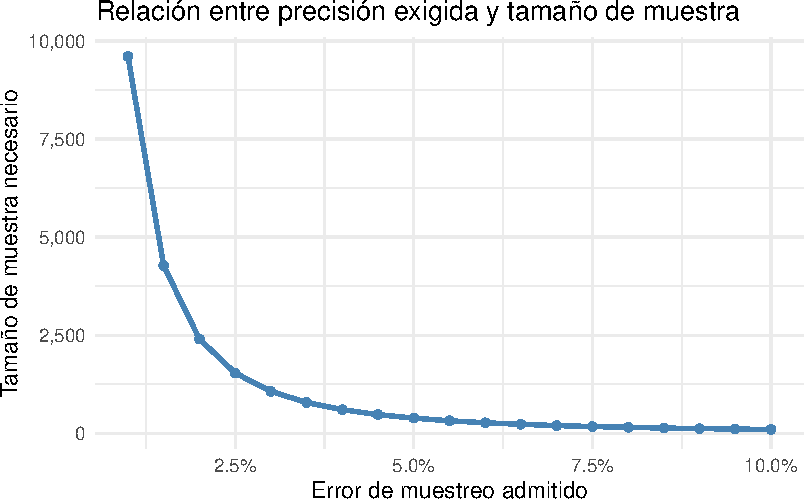
\includegraphics[keepaspectratio]{09-encuestas-muestreo_files/figure-pdf/grafico-tamano-muestral-1.pdf}}

}

\caption{Tamaño de muestra necesario en función del error de muestreo
admitido (confianza del 95\%, p = 0.5).}

\end{figure}%

Como cabía esperar, el tamaño de muestra necesario crece muy rápidamente
a medida que se exige un error de muestreo menor, debido a la relación
cuadrática entre ambas cantidades.

\subsection{Comparación entre muestreo aleatorio simple y muestreo
estratificado}\label{comparaciuxf3n-entre-muestreo-aleatorio-simple-y-muestreo-estratificado}

Para comparar la precisión del muestreo aleatorio simple (MAS) frente al
muestreo estratificado, se simula una ``población'' de \(N=4000\)
personas repartidas en 4 regiones, con una opinión binaria (a favor / en
contra de una medida) cuya prevalencia varía sustancialmente de una
región a otra, de forma que la región constituye un buen criterio de
estratificación:

\begin{Shaded}
\begin{Highlighting}[]
\FunctionTok{set.seed}\NormalTok{(}\DecValTok{2026}\NormalTok{)}
\NormalTok{N }\OtherTok{\textless{}{-}} \DecValTok{4000}

\NormalTok{poblacion }\OtherTok{\textless{}{-}} \FunctionTok{tibble}\NormalTok{(}
  \AttributeTok{id =} \DecValTok{1}\SpecialCharTok{:}\NormalTok{N,}
  \AttributeTok{region =} \FunctionTok{sample}\NormalTok{(}
    \FunctionTok{c}\NormalTok{(}\StringTok{"Norte"}\NormalTok{, }\StringTok{"Sur"}\NormalTok{, }\StringTok{"Este"}\NormalTok{, }\StringTok{"Oeste"}\NormalTok{),}
    \AttributeTok{size =}\NormalTok{ N,}
    \AttributeTok{replace =} \ConstantTok{TRUE}\NormalTok{,}
    \AttributeTok{prob =} \FunctionTok{c}\NormalTok{(}\FloatTok{0.30}\NormalTok{, }\FloatTok{0.25}\NormalTok{, }\FloatTok{0.25}\NormalTok{, }\FloatTok{0.20}\NormalTok{)}
\NormalTok{  )}
\NormalTok{)}

\CommentTok{\# La probabilidad de estar a favor depende fuertemente de la región}
\NormalTok{prob\_favor }\OtherTok{\textless{}{-}} \FunctionTok{c}\NormalTok{(}\AttributeTok{Norte =} \FloatTok{0.75}\NormalTok{, }\AttributeTok{Sur =} \FloatTok{0.30}\NormalTok{, }\AttributeTok{Este =} \FloatTok{0.55}\NormalTok{, }\AttributeTok{Oeste =} \FloatTok{0.40}\NormalTok{)}

\NormalTok{poblacion }\OtherTok{\textless{}{-}}\NormalTok{ poblacion }\SpecialCharTok{|\textgreater{}}
  \FunctionTok{mutate}\NormalTok{(}
    \AttributeTok{p\_favor =}\NormalTok{ prob\_favor[region],}
    \AttributeTok{opinion =} \FunctionTok{rbinom}\NormalTok{(N, }\AttributeTok{size =} \DecValTok{1}\NormalTok{, }\AttributeTok{prob =}\NormalTok{ p\_favor),}
    \AttributeTok{opinion =} \FunctionTok{factor}\NormalTok{(opinion, }\AttributeTok{levels =} \FunctionTok{c}\NormalTok{(}\DecValTok{0}\NormalTok{, }\DecValTok{1}\NormalTok{), }\AttributeTok{labels =} \FunctionTok{c}\NormalTok{(}\StringTok{"En contra"}\NormalTok{, }\StringTok{"A favor"}\NormalTok{))}
\NormalTok{  )}

\NormalTok{poblacion}
\end{Highlighting}
\end{Shaded}

\begin{verbatim}
# A tibble: 4,000 x 4
      id region p_favor opinion  
   <int> <chr>    <dbl> <fct>    
 1     1 Sur       0.3  En contra
 2     2 Sur       0.3  En contra
 3     3 Norte     0.75 A favor  
 4     4 Norte     0.75 A favor  
 5     5 Sur       0.3  En contra
 6     6 Norte     0.75 A favor  
 7     7 Este      0.55 A favor  
 8     8 Oeste     0.4  A favor  
 9     9 Norte     0.75 A favor  
10    10 Sur       0.3  A favor  
# i 3,990 more rows
\end{verbatim}

La proporción real de personas a favor en el conjunto de la población
(el parámetro que se desea estimar) es:

\begin{Shaded}
\begin{Highlighting}[]
\NormalTok{p\_poblacional }\OtherTok{\textless{}{-}} \FunctionTok{mean}\NormalTok{(poblacion}\SpecialCharTok{$}\NormalTok{opinion }\SpecialCharTok{==} \StringTok{"A favor"}\NormalTok{)}
\NormalTok{p\_poblacional}
\end{Highlighting}
\end{Shaded}

\begin{verbatim}
[1] 0.51325
\end{verbatim}

A partir de esta población se extrae, en primer lugar, una muestra
aleatoria simple de \(n=1068\) individuos:

\begin{Shaded}
\begin{Highlighting}[]
\NormalTok{muestra\_mas }\OtherTok{\textless{}{-}}\NormalTok{ poblacion }\SpecialCharTok{|\textgreater{}}
  \FunctionTok{slice\_sample}\NormalTok{(}\AttributeTok{n =}\NormalTok{ n\_necesario)}

\NormalTok{p\_mas }\OtherTok{\textless{}{-}} \FunctionTok{mean}\NormalTok{(muestra\_mas}\SpecialCharTok{$}\NormalTok{opinion }\SpecialCharTok{==} \StringTok{"A favor"}\NormalTok{)}
\NormalTok{p\_mas}
\end{Highlighting}
\end{Shaded}

\begin{verbatim}
[1] 0.5065543
\end{verbatim}

A continuación se extrae una muestra estratificada por región, con
afijación proporcional, del mismo tamaño total aproximado: se calcula la
proporción que representa cada región en la población y se selecciona
ese mismo porcentaje dentro de cada estrato:

\begin{Shaded}
\begin{Highlighting}[]
\NormalTok{prop\_muestral }\OtherTok{\textless{}{-}}\NormalTok{ n\_necesario }\SpecialCharTok{/}\NormalTok{ N}

\NormalTok{muestra\_estratificada }\OtherTok{\textless{}{-}}\NormalTok{ poblacion }\SpecialCharTok{|\textgreater{}}
  \FunctionTok{group\_by}\NormalTok{(region) }\SpecialCharTok{|\textgreater{}}
  \FunctionTok{slice\_sample}\NormalTok{(}\AttributeTok{prop =}\NormalTok{ prop\_muestral) }\SpecialCharTok{|\textgreater{}}
  \FunctionTok{ungroup}\NormalTok{()}

\FunctionTok{nrow}\NormalTok{(muestra\_estratificada)}
\end{Highlighting}
\end{Shaded}

\begin{verbatim}
[1] 1067
\end{verbatim}

\begin{Shaded}
\begin{Highlighting}[]
\NormalTok{p\_estratificado }\OtherTok{\textless{}{-}} \FunctionTok{mean}\NormalTok{(muestra\_estratificada}\SpecialCharTok{$}\NormalTok{opinion }\SpecialCharTok{==} \StringTok{"A favor"}\NormalTok{)}
\NormalTok{p\_estratificado}
\end{Highlighting}
\end{Shaded}

\begin{verbatim}
[1] 0.5126523
\end{verbatim}

Se comprueba que la muestra estratificada respeta, aproximadamente, el
peso de cada región en la población:

\begin{Shaded}
\begin{Highlighting}[]
\NormalTok{muestra\_estratificada }\SpecialCharTok{|\textgreater{}}
  \FunctionTok{count}\NormalTok{(region) }\SpecialCharTok{|\textgreater{}}
  \FunctionTok{mutate}\NormalTok{(}\AttributeTok{proporcion\_muestra =}\NormalTok{ n }\SpecialCharTok{/} \FunctionTok{sum}\NormalTok{(n))}
\end{Highlighting}
\end{Shaded}

\begin{verbatim}
# A tibble: 4 x 3
  region     n proporcion_muestra
  <chr>  <int>              <dbl>
1 Este     268              0.251
2 Norte    322              0.302
3 Oeste    205              0.192
4 Sur      272              0.255
\end{verbatim}

\begin{Shaded}
\begin{Highlighting}[]
\NormalTok{poblacion }\SpecialCharTok{|\textgreater{}}
  \FunctionTok{count}\NormalTok{(region) }\SpecialCharTok{|\textgreater{}}
  \FunctionTok{mutate}\NormalTok{(}\AttributeTok{proporcion\_poblacion =}\NormalTok{ n }\SpecialCharTok{/} \FunctionTok{sum}\NormalTok{(n))}
\end{Highlighting}
\end{Shaded}

\begin{verbatim}
# A tibble: 4 x 3
  region     n proporcion_poblacion
  <chr>  <int>                <dbl>
1 Este    1004                0.251
2 Norte   1207                0.302
3 Oeste    769                0.192
4 Sur     1020                0.255
\end{verbatim}

Por último, se comparan gráficamente las tres proporciones: la real de
la población y las estimadas por cada uno de los dos métodos de
muestreo.

\begin{Shaded}
\begin{Highlighting}[]
\NormalTok{comparacion }\OtherTok{\textless{}{-}} \FunctionTok{tibble}\NormalTok{(}
  \AttributeTok{metodo =} \FunctionTok{c}\NormalTok{(}\StringTok{"Población"}\NormalTok{, }\StringTok{"MAS"}\NormalTok{, }\StringTok{"Estratificado"}\NormalTok{),}
  \AttributeTok{proporcion =} \FunctionTok{c}\NormalTok{(p\_poblacional, p\_mas, p\_estratificado)}
\NormalTok{) }\SpecialCharTok{|\textgreater{}}
  \FunctionTok{mutate}\NormalTok{(}\AttributeTok{metodo =} \FunctionTok{factor}\NormalTok{(metodo, }\AttributeTok{levels =} \FunctionTok{c}\NormalTok{(}\StringTok{"Población"}\NormalTok{, }\StringTok{"MAS"}\NormalTok{, }\StringTok{"Estratificado"}\NormalTok{)))}

\FunctionTok{ggplot}\NormalTok{(comparacion, }\FunctionTok{aes}\NormalTok{(}\AttributeTok{x =}\NormalTok{ metodo, }\AttributeTok{y =}\NormalTok{ proporcion, }\AttributeTok{fill =}\NormalTok{ metodo)) }\SpecialCharTok{+}
  \FunctionTok{geom\_col}\NormalTok{(}\AttributeTok{width =} \FloatTok{0.6}\NormalTok{) }\SpecialCharTok{+}
  \FunctionTok{geom\_hline}\NormalTok{(}\AttributeTok{yintercept =}\NormalTok{ p\_poblacional, }\AttributeTok{linetype =} \StringTok{"dashed"}\NormalTok{, }\AttributeTok{color =} \StringTok{"gray30"}\NormalTok{) }\SpecialCharTok{+}
  \FunctionTok{scale\_y\_continuous}\NormalTok{(}\AttributeTok{labels =}\NormalTok{ scales}\SpecialCharTok{::}\FunctionTok{percent\_format}\NormalTok{()) }\SpecialCharTok{+}
  \FunctionTok{scale\_fill\_brewer}\NormalTok{(}\AttributeTok{palette =} \StringTok{"Set2"}\NormalTok{) }\SpecialCharTok{+}
  \FunctionTok{labs}\NormalTok{(}
    \AttributeTok{x =} \ConstantTok{NULL}\NormalTok{,}
    \AttributeTok{y =} \StringTok{"Proporción a favor"}\NormalTok{,}
    \AttributeTok{title =} \StringTok{"Estimación de la proporción según el diseño de muestreo"}
\NormalTok{  ) }\SpecialCharTok{+}
  \FunctionTok{theme\_minimal}\NormalTok{() }\SpecialCharTok{+}
  \FunctionTok{theme}\NormalTok{(}\AttributeTok{legend.position =} \StringTok{"none"}\NormalTok{)}
\end{Highlighting}
\end{Shaded}

\begin{figure}[H]

{\centering \pandocbounded{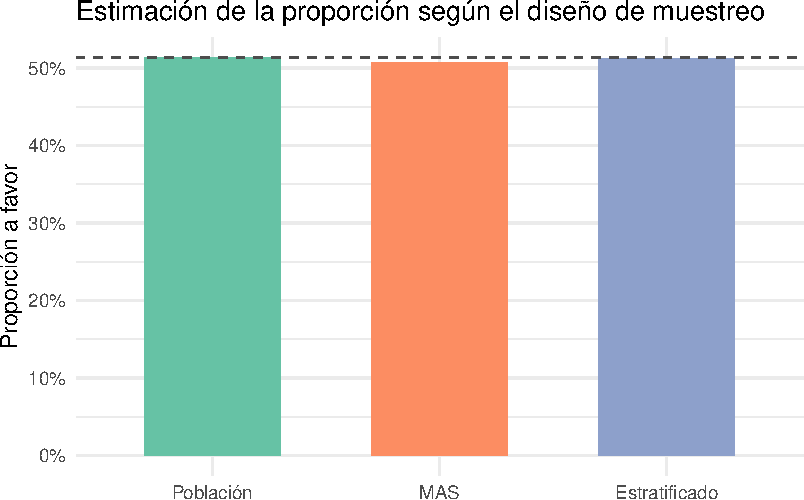
\includegraphics[keepaspectratio]{09-encuestas-muestreo_files/figure-pdf/grafico-comparacion-1.pdf}}

}

\caption{Proporción de personas a favor de la medida: valor poblacional
real frente a las estimaciones por muestreo aleatorio simple y por
muestreo estratificado.}

\end{figure}%

En esta simulación, la proporción real de personas a favor en la
población es del 51.3\%, mientras que la muestra aleatoria simple estima
un 50.7\% y la muestra estratificada un 51.3\%. Dado que la región está
fuertemente relacionada con la opinión (los estratos son internamente
bastante homogéneos) y que la afijación proporcional garantiza que cada
región esté representada en su peso exacto, cabe esperar que, en
promedio y a lo largo de repeticiones del muestreo, la estimación
estratificada se aproxime más a la proporción poblacional que la del
muestreo aleatorio simple, cuya composición por regiones puede variar de
una muestra a otra por puro azar. Este es precisamente el motivo por el
que, siempre que se disponga de una variable de estratificación
adecuada, el muestreo estratificado suele preferirse al muestreo
aleatorio simple en las encuestas reales.

\section{Cuándo utilizar este
diseño}\label{cuuxe1ndo-utilizar-este-diseuxf1o-7}

El diseño de muestreo no es un tipo de estudio alternativo a los
descritos en los capítulos anteriores, sino una dimensión transversal a
todos ellos: tanto un \hyperref[estudios-descriptivos]{estudio
descriptivo} como un \hyperref[estudios-transversales]{estudio
transversal}, un \hyperref[estudios-de-cohortes]{estudio de cohortes} o
un ensayo \hyperref[estudios-experimentales]{experimental} necesitan
seleccionar en algún momento una muestra de la población, y la calidad
de ese muestreo condiciona directamente la validez de las conclusiones
que se extraigan. Conviene prestar especial atención al diseño muestral,
y en particular optar por el muestreo estratificado o por conglomerados
frente al muestreo aleatorio simple, cuando la población es muy
heterogénea, cuando existen variables conocidas fuertemente relacionadas
con el fenómeno de interés, o cuando el coste de acceder a los
individuos varía mucho según su localización o su pertenencia a un
determinado grupo. Un cálculo previo del tamaño muestral necesario, en
función de la precisión exigida y de los recursos disponibles, es
también un paso imprescindible en la planificación de cualquier estudio,
se trate de una encuesta de opinión, un estudio epidemiológico o un
ensayo clínico. En definitiva, ningún análisis estadístico posterior,
por sofisticado que sea, puede compensar una muestra mal seleccionada:
la calidad del diseño muestral es, junto con el propio diseño del
estudio, uno de los pilares sobre los que se sostiene la validez de
cualquier investigación estadística.

\part{Selección del contraste estadístico}

\chapter{Selección del contraste
estadístico}\label{selecciuxf3n-del-contraste-estaduxedstico-1}

Los capítulos anteriores han mostrado cómo \textbf{diseñar} un estudio
estadístico: cómo seleccionar la muestra, cómo asignar (o no) la
exposición, y en qué momentos recoger los datos. Una vez recogidos los
datos según alguno de esos diseños, queda una segunda pregunta, igual de
importante: ¿qué \textbf{contraste de hipótesis} es el adecuado para
analizarlos?

La respuesta depende, sobre todo, de tres factores:

\begin{itemize}
\tightlist
\item
  El \textbf{número de variables} que intervienen en el estudio y, si
  hay más de una, cuál es la variable dependiente (la respuesta que se
  quiere explicar) y cuál la independiente (el factor que se cree que
  influye en ella).
\item
  El \textbf{tipo de las variables}: cuantitativas, cualitativas
  ordinales o cualitativas nominales.
\item
  La \textbf{naturaleza de las poblaciones o grupos comparados}: si son
  independientes (individuos distintos en cada grupo) o están
  relacionadas o pareadas (los mismos individuos medidos varias veces, o
  emparejados de algún modo).
\end{itemize}

Esta segunda parte del libro está dedicada precisamente a esta cuestión:
cómo elegir, y cómo ejecutar en R, el contraste de hipótesis apropiado
en cada situación. A diferencia de la primera parte, aquí el capítulo no
se organiza por tipo de diseño de investigación, sino por el
\textbf{número y la naturaleza de las poblaciones o grupos} que se
comparan, que es el criterio que realmente determina qué contraste
utilizar. El diseño del estudio (si los datos proceden de un
\hyperref[estudios-de-cohortes]{estudio de cohortes}, de un
\hyperref[estudios-experimentales]{ensayo clínico} o de una simple
\hyperref[encuestas-y-diseuxf1o-de-muestreo]{encuesta}) influye en qué
conclusiones de causalidad pueden extraerse del resultado del contraste,
pero no cambia, en general, qué contraste es el adecuado: eso lo
determinan el número de variables, su tipo, y si las poblaciones
comparadas son independientes o están pareadas.

\section{Tabla de decisión}\label{tabla-de-decisiuxf3n}

La siguiente tabla resume los contrastes de hipótesis más habituales
según estos criterios, y sirve como mapa de esta segunda parte del
libro. Cada fila indica, para una combinación de variable(s)
independiente(s), variable dependiente y objetivo del análisis, cuál es
el contraste apropiado y en qué capítulo se desarrolla.

Variables independientes

Variable dependiente

Objetivo

Contraste

Capítulo

Ninguna (una población)

Cuantitativa

Contrastar la normalidad de una variable

Kolmogorov-Smirnov (muestras grandes) / Shapiro-Wilk

\href{11-contrastes-una-poblacion.qmd}{Contrastes para una población}

Cuantitativa normal

Contrastar si la media poblacional tiene un valor determinado

Test t para la media de una población

Ninguna (una población)

Cualitativa (2 categorías)

Contrastar si la proporción de una categoría tiene un valor determinado

Test binomial / Test Z para una proporción

Cualitativa (\textgreater2 categorías)

Contrastar si las proporciones de las categorías tienen unos valores
determinados

Test Chi-cuadrado de bondad de ajuste

Una cualitativa con 2 categorías, poblaciones independientes

Cuantitativa normal

Contrastar si hay diferencias entre las medias de las dos poblaciones

Test F de Fisher (varianzas) + Test t de comparación de medias

\href{12-contrastes-dos-poblaciones-independientes.qmd}{Contrastes para
dos poblaciones independientes}

Cuantitativa o cualitativa ordinal

Contrastar si hay diferencias entre las distribuciones de las dos
poblaciones

Test U de Mann-Whitney

Cualitativa (2 categorías)

Contrastar si hay relación entre las variables o diferencias entre
proporciones

Test Chi-cuadrado de independencia / Test exacto de Fisher

Cualitativa (\textgreater2 categorías)

Contrastar si hay relación entre las variables o diferencias entre
proporciones

Test Chi-cuadrado de independencia

Una cualitativa con \textgreater2 categorías, poblaciones independientes

Cuantitativa normal (varianzas homogéneas)

Contrastar si hay diferencias entre las medias de las poblaciones

Levene (varianzas) + ANOVA de un factor + Tukey/Bonferroni

Cuantitativa o cualitativa ordinal

Contrastar si hay diferencias entre las distribuciones de las
poblaciones

Test de Kruskal-Wallis + comparaciones por pares de Wilcoxon

Una cualitativa con 2 categorías, poblaciones pareadas

Cuantitativa normal

Contrastar si hay diferencias entre las medias de las dos poblaciones
pareadas

Test t para datos pareados

\href{13-contrastes-dos-poblaciones-pareadas.qmd}{Contrastes para dos
poblaciones pareadas}

Cuantitativa o cualitativa ordinal

Contrastar si hay diferencias entre las distribuciones de las dos
poblaciones pareadas

Test de Wilcoxon para datos pareados

Cualitativa (2 categorías)

Contrastar si hay diferencias entre las proporciones de las dos
poblaciones pareadas

Test de McNemar

Una cualitativa con \textgreater2 categorías, poblaciones relacionadas
(medidas repetidas)

Cuantitativa normal

Contrastar si hay diferencias entre las medidas repetidas

ANOVA de medidas repetidas de un factor

\href{15-contrastes-medidas-repetidas.qmd}{Contrastes para más de dos
poblaciones relacionadas}

Cuantitativa o cualitativa ordinal

Contrastar si hay diferencias entre las medidas repetidas

Test de Friedman

Una cuantitativa normal

Cuantitativa normal

Contrastar si existe relación lineal / construir un modelo predictivo

Correlación de Pearson / Regresión simple

\href{16-relacion-entre-variables.qmd}{Relación y predicción entre dos
variables}

Cuantitativa o cualitativa ordinal

Contrastar si existe relación (de orden) entre las dos variables

Correlación de Spearman

Una cuantitativa

Cualitativa (2 categorías)

Construir un modelo predictivo que explique la variable cualitativa

Regresión logística simple

\begin{tcolorbox}[enhanced jigsaw, arc=.35mm, bottomrule=.15mm, bottomtitle=1mm, breakable, colback=white, colbacktitle=quarto-callout-note-color!10!white, colframe=quarto-callout-note-color-frame, coltitle=black, left=2mm, leftrule=.75mm, opacityback=0, opacitybacktitle=0.6, rightrule=.15mm, title=\textcolor{quarto-callout-note-color}{\faInfo}\hspace{0.5em}{Nota}, titlerule=0mm, toprule=.15mm, toptitle=1mm]

Esta tabla no agota todas las situaciones posibles. Quedan fuera de esta
segunda parte, por ser casos más especializados, los contrastes de
\textbf{concordancia o acuerdo entre dos medidas} de un mismo fenómeno
(como el coeficiente Kappa de Cohen para variables cualitativas o el
coeficiente de correlación intraclase para variables cuantitativas), así
como el ANOVA de dos o más factores y sus interacciones. El
\href{https://aprendeconalf.es/estadistica-manual/}{Manual de
Estadística} desarrolla además, con mucho más detalle, la correlación y
la regresión, y el coeficiente chi-cuadrado y de contingencia entre
variables cualitativas, por lo que el último capítulo de esta parte
remite a él para profundizar en esos contrastes en lugar de repetir aquí
su desarrollo.

\end{tcolorbox}

\section{El conjunto de datos de
ejemplo}\label{el-conjunto-de-datos-de-ejemplo}

Todos los ejemplos de esta segunda parte utilizan un mismo conjunto de
datos, \texttt{datos-curso.csv}, con las calificaciones de 120 alumnos
de una asignatura dividida en tres grupos de clase. Se puede descargar
desde el repositorio del libro para reproducir los ejemplos.

\begin{Shaded}
\begin{Highlighting}[]
\NormalTok{df }\OtherTok{\textless{}{-}} \FunctionTok{read\_csv}\NormalTok{(}\StringTok{"datos/datos{-}curso.csv"}\NormalTok{)}
\end{Highlighting}
\end{Shaded}

\begin{verbatim}
Rows: 120 Columns: 16
-- Column specification --------------------------------------------------------
Delimiter: ","
chr (9): sexo, turno, grupo, trabaja, calificacionA, calificacionB, califica...
dbl (7): notaA, notaB, notaC, notaD, notaE, asinaturas.aprobadas, nota.media

i Use `spec()` to retrieve the full column specification for this data.
i Specify the column types or set `show_col_types = FALSE` to quiet this message.
\end{verbatim}

\begin{Shaded}
\begin{Highlighting}[]
\FunctionTok{glimpse}\NormalTok{(df)}
\end{Highlighting}
\end{Shaded}

\begin{verbatim}
Rows: 120
Columns: 16
$ sexo                 <chr> "Mujer", "Hombre", "Hombre", "Hombre", "Hombre", ~
$ turno                <chr> "Tarde", "Mañana", "Mañana", "Mañana", "Mañana", ~
$ grupo                <chr> "C", "A", "B", "B", "A", "A", "A", "C", "C", "C",~
$ trabaja              <chr> "N", "N", "N", "N", "N", "S", "N", "S", "N", "N",~
$ notaA                <dbl> 5.2, 5.7, 8.3, 6.1, 6.2, 8.6, 6.7, 4.1, 5.0, 5.3,~
$ notaB                <dbl> 6.3, 5.7, 8.8, 6.8, 9.0, 8.9, 7.9, 5.2, 5.0, 6.3,~
$ notaC                <dbl> 3.4, 4.2, 8.8, 4.0, 5.0, 9.5, 5.6, 1.7, 3.3, 4.8,~
$ notaD                <dbl> 2.3, 3.5, 8.0, 3.5, 4.4, 8.4, 4.8, 0.3, 2.7, 3.6,~
$ notaE                <dbl> 2.0, 2.7, 5.5, 2.2, 3.7, 3.9, 4.2, 1.0, 6.0, 2.3,~
$ calificacionA        <chr> "Aprobado", "Aprobado", "Aprobado", "Aprobado", "~
$ calificacionB        <chr> "Aprobado", "Aprobado", "Aprobado", "Aprobado", "~
$ calificacionC        <chr> "Suspenso", "Suspenso", "Aprobado", "Suspenso", "~
$ calificacionD        <chr> "Suspenso", "Suspenso", "Aprobado", "Suspenso", "~
$ calificacionE        <chr> "Suspenso", "Suspenso", "Aprobado", "Suspenso", "~
$ asinaturas.aprobadas <dbl> 2, 2, 5, 2, 3, 4, 3, 1, 2, 2, 3, 2, 3, 3, 3, 4, 4~
$ nota.media           <dbl> 3.8, 4.3, 7.9, 4.5, 5.7, 7.8, 5.8, 2.5, 4.4, 4.5,~
\end{verbatim}

Las variables que contiene son:

{\def\LTcaptype{none} % do not increment counter
\begin{longtable}[]{@{}
  >{\raggedright\arraybackslash}p{(\linewidth - 2\tabcolsep) * \real{0.5000}}
  >{\raggedright\arraybackslash}p{(\linewidth - 2\tabcolsep) * \real{0.5000}}@{}}
\toprule\noalign{}
\begin{minipage}[b]{\linewidth}\raggedright
Variable
\end{minipage} & \begin{minipage}[b]{\linewidth}\raggedright
Descripción
\end{minipage} \\
\midrule\noalign{}
\endhead
\bottomrule\noalign{}
\endlastfoot
\texttt{sexo} & Sexo del alumno (Hombre / Mujer). \\
\texttt{turno} & Turno en el que cursa la asignatura (Mañana /
Tarde). \\
\texttt{grupo} & Grupo de clase al que pertenece (A, B o C). \\
\texttt{trabaja} & Si el alumno compagina los estudios con un trabajo (S
/ N). \\
\texttt{notaA}, \ldots, \texttt{notaE} & Calificación numérica (0-10)
obtenida en cinco pruebas o exámenes distintos de la asignatura. \\
\texttt{calificacionA}, \ldots, \texttt{calificacionE} & Resultado
cualitativo (Aprobado / Suspenso) de cada una de esas cinco pruebas. \\
\texttt{asinaturas.aprobadas} & Número de asignaturas aprobadas por el
alumno ese curso (0 a 5). \\
\texttt{nota.media} & Nota media del alumno en el curso. \\
\end{longtable}
}

Este conjunto de datos permite ilustrar tanto comparaciones entre
\textbf{poblaciones independientes} (por ejemplo, comparar
\texttt{notaA} entre hombres y mujeres, dos grupos de individuos
distintos) como comparaciones entre \textbf{poblaciones pareadas o
medidas repetidas} (por ejemplo, comparar \texttt{notaA} con
\texttt{notaB} para los mismos alumnos, o las cinco notas \texttt{notaA}
a \texttt{notaE} de cada alumno entre sí).

\section{Estructura de los
capítulos}\label{estructura-de-los-capuxedtulos}

Los capítulos siguientes están organizados por el número de poblaciones
o grupos comparados y por si estos son independientes o están
relacionados, siguiendo el orden de la tabla de decisión anterior. Cada
contraste se presenta con una estructura fija: el \textbf{objetivo} del
contraste, sus \textbf{requisitos} de aplicación, la \textbf{hipótesis
nula} que pone a prueba, un ejemplo resuelto sobre el conjunto de datos
del curso, y la interpretación del resultado.

\chapter{Contrastes para una
población}\label{contrastes-para-una-poblaciuxf3n}

Este primer capítulo de la segunda parte del libro corresponde a la fila
más sencilla de la
\hyperref[selecciuxf3n-del-contraste-estaduxedstico-1]{tabla de
decisión}: no hay ninguna variable independiente, y el objetivo es
describir o contrastar una única variable de una única población, sin
compararla con ninguna otra. Según el tipo de esa variable, cuantitativa
o cualitativa, los estadísticos descriptivos, los gráficos y los
contrastes de hipótesis apropiados son distintos, por lo que el capítulo
se organiza en dos grandes secciones. Todos los ejemplos utilizan el
conjunto de datos \texttt{datos-curso.csv} presentado en el capítulo
anterior.

\section{Una variable cuantitativa}\label{una-variable-cuantitativa}

\subsection{Estadísticos
descriptivos}\label{estaduxedsticos-descriptivos}

Antes de aplicar cualquier contraste conviene describir la variable con
sus estadísticos habituales de posición, dispersión y forma. Para la
variable \texttt{notaA} se obtienen así:

\begin{Shaded}
\begin{Highlighting}[]
\FunctionTok{nrow}\NormalTok{(df)}
\end{Highlighting}
\end{Shaded}

\begin{verbatim}
[1] 120
\end{verbatim}

\begin{Shaded}
\begin{Highlighting}[]
\FunctionTok{mean}\NormalTok{(df}\SpecialCharTok{$}\NormalTok{notaA)}
\end{Highlighting}
\end{Shaded}

\begin{verbatim}
[1] 6.028333
\end{verbatim}

\begin{Shaded}
\begin{Highlighting}[]
\FunctionTok{sd}\NormalTok{(df}\SpecialCharTok{$}\NormalTok{notaA)}
\end{Highlighting}
\end{Shaded}

\begin{verbatim}
[1] 1.340524
\end{verbatim}

\begin{Shaded}
\begin{Highlighting}[]
\FunctionTok{min}\NormalTok{(df}\SpecialCharTok{$}\NormalTok{notaA)}
\end{Highlighting}
\end{Shaded}

\begin{verbatim}
[1] 2.5
\end{verbatim}

\begin{Shaded}
\begin{Highlighting}[]
\FunctionTok{max}\NormalTok{(df}\SpecialCharTok{$}\NormalTok{notaA)}
\end{Highlighting}
\end{Shaded}

\begin{verbatim}
[1] 9.3
\end{verbatim}

\begin{Shaded}
\begin{Highlighting}[]
\FunctionTok{quantile}\NormalTok{(df}\SpecialCharTok{$}\NormalTok{notaA)}
\end{Highlighting}
\end{Shaded}

\begin{verbatim}
   0%   25%   50%   75%  100% 
2.500 5.100 5.900 6.825 9.300 
\end{verbatim}

\begin{Shaded}
\begin{Highlighting}[]
\FunctionTok{library}\NormalTok{(moments)}
\FunctionTok{skewness}\NormalTok{(df}\SpecialCharTok{$}\NormalTok{notaA)}
\end{Highlighting}
\end{Shaded}

\begin{verbatim}
[1] 0.1373915
\end{verbatim}

\begin{Shaded}
\begin{Highlighting}[]
\FunctionTok{kurtosis}\NormalTok{(df}\SpecialCharTok{$}\NormalTok{notaA) }\SpecialCharTok{{-}} \DecValTok{3}
\end{Highlighting}
\end{Shaded}

\begin{verbatim}
[1] -0.102287
\end{verbatim}

La muestra está formada por los \(n=120\) alumnos del curso, con una
nota media en la prueba A de \(\bar{x}=6.03\) y una desviación típica de
\(s=1.34\). Las calificaciones oscilan entre un mínimo de 2.5 y un
máximo de 9.3, con una mediana de 5.9 y un rango intercuartílico que va
de \(Q_1=5.1\) a \(Q_3=6.83\). El coeficiente de asimetría es
prácticamente nulo (\(0.137\)), lo que indica una distribución casi
simétrica con una ligerísima cola hacia la derecha, y el coeficiente de
apuntamiento (curtosis menos 3) también es cercano a cero (\(-0.102\)),
por lo que la distribución no se aparta mucho de la forma acampanada de
una normal. Estos dos últimos valores ya anticipan el resultado del
contraste de normalidad que se aplica más adelante.

\subsection{Gráficos}\label{gruxe1ficos}

El histograma y el diagrama de caja y bigotes son las representaciones
habituales de una variable cuantitativa, y permiten valorar visualmente
la forma de la distribución (simetría, apuntamiento, posibles valores
atípicos) antes de someterla a un contraste formal.

\begin{Shaded}
\begin{Highlighting}[]
\FunctionTok{ggplot}\NormalTok{(df, }\FunctionTok{aes}\NormalTok{(}\AttributeTok{x =}\NormalTok{ notaA)) }\SpecialCharTok{+}
  \FunctionTok{geom\_histogram}\NormalTok{(}\AttributeTok{binwidth =} \DecValTok{1}\NormalTok{, }\AttributeTok{fill =} \StringTok{"steelblue"}\NormalTok{, }\AttributeTok{color =} \StringTok{"white"}\NormalTok{) }\SpecialCharTok{+}
  \FunctionTok{labs}\NormalTok{(}\AttributeTok{x =} \StringTok{"Nota A"}\NormalTok{, }\AttributeTok{y =} \StringTok{"Frecuencia"}\NormalTok{)}
\end{Highlighting}
\end{Shaded}

\pandocbounded{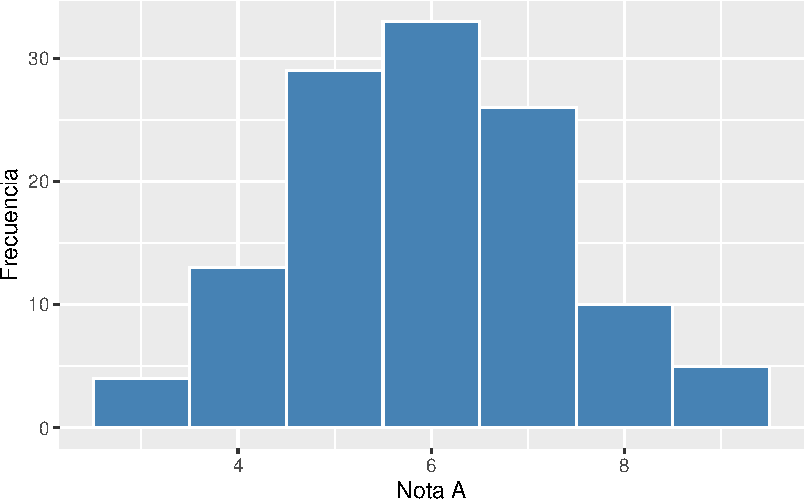
\includegraphics[keepaspectratio]{11-contrastes-una-poblacion_files/figure-pdf/unnamed-chunk-3-1.pdf}}

\begin{Shaded}
\begin{Highlighting}[]
\FunctionTok{ggplot}\NormalTok{(df, }\FunctionTok{aes}\NormalTok{(}\AttributeTok{y =}\NormalTok{ notaA)) }\SpecialCharTok{+}
  \FunctionTok{geom\_boxplot}\NormalTok{(}\AttributeTok{fill =} \StringTok{"steelblue"}\NormalTok{) }\SpecialCharTok{+}
  \FunctionTok{labs}\NormalTok{(}\AttributeTok{y =} \StringTok{"Nota A"}\NormalTok{)}
\end{Highlighting}
\end{Shaded}

\pandocbounded{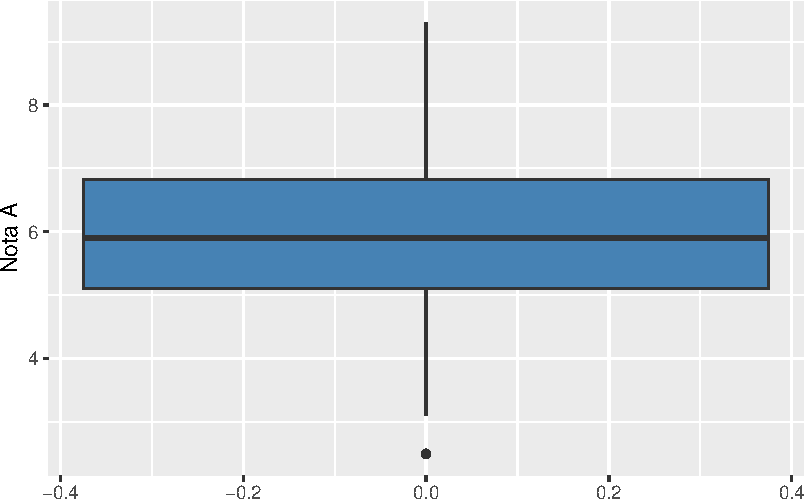
\includegraphics[keepaspectratio]{11-contrastes-una-poblacion_files/figure-pdf/unnamed-chunk-4-1.pdf}}

Ambos gráficos confirman lo que ya sugerían los estadísticos
descriptivos: una distribución razonablemente simétrica y centrada
alrededor de 6, sin valores atípicos destacables en el diagrama de caja.

\subsection{Contraste de normalidad de
Shapiro-Wilk}\label{contraste-de-normalidad-de-shapiro-wilk}

\begin{definition}[Contraste de normalidad de
Shapiro-Wilk]\protect\hypertarget{def-unapoblacion-shapiro-wilk}{}\label{def-unapoblacion-shapiro-wilk}

El contraste de Shapiro-Wilk permite comprobar si una muestra de una
variable cuantitativa procede de una población con distribución normal.
Su hipótesis nula es

\[H_0: \text{la variable sigue una distribución normal.}\]

Se rechaza esta hipótesis cuando el p-valor del contraste es menor que
el nivel de significación fijado (habitualmente 0.05).

\end{definition}

\textbf{Requisitos}: una variable cuantitativa. El test de Shapiro-Wilk
funciona bien con cualquier tamaño muestral, aunque con muestras muy
grandes es tan potente que puede rechazar la normalidad ante
desviaciones mínimas y sin relevancia práctica; en ese caso es
preferible el contraste de Kolmogorov-Smirnov (\texttt{ks.test()}), que
compara la función de distribución empírica de los datos con la de una
normal teórica y es más adecuado para muestras grandes.

Muchos de los contrastes que se estudian en este libro, como el test t,
exigen que la variable analizada siga una distribución normal (o que la
muestra sea suficientemente grande, \(n \geq 30\), para invocar el
teorema central del límite). El contraste de Shapiro-Wilk es la
herramienta habitual para comprobar ese requisito antes de aplicarlos. A
continuación se contrasta la normalidad de dos variables del conjunto de
datos, \texttt{notaA} y \texttt{notaE}, para mostrar un caso en el que
no se rechaza la normalidad y otro en el que sí se rechaza.

\begin{example}[]\protect\hypertarget{exm-unapoblacion-shapiro-wilk}{}\label{exm-unapoblacion-shapiro-wilk}

~

\begin{Shaded}
\begin{Highlighting}[]
\FunctionTok{shapiro.test}\NormalTok{(df}\SpecialCharTok{$}\NormalTok{notaA)}
\end{Highlighting}
\end{Shaded}

\begin{verbatim}

    Shapiro-Wilk normality test

data:  df$notaA
W = 0.99424, p-value = 0.907
\end{verbatim}

\begin{Shaded}
\begin{Highlighting}[]
\FunctionTok{shapiro.test}\NormalTok{(df}\SpecialCharTok{$}\NormalTok{notaE)}
\end{Highlighting}
\end{Shaded}

\begin{verbatim}

    Shapiro-Wilk normality test

data:  df$notaE
W = 0.92264, p-value = 4.065e-06
\end{verbatim}

Para \texttt{notaA} el estadístico es \(W=0.994\) con un p-valor de
\(0.907\), muy superior a 0.05, por lo que no hay evidencia para
rechazar \(H_0\): es razonable asumir que \texttt{notaA} sigue una
distribución normal. Para \texttt{notaE}, en cambio, el p-valor es
\(4.07\times10^{-6}\), muy inferior a 0.05, por lo que se rechaza
\(H_0\) y se concluye que \texttt{notaE} no sigue una distribución
normal (coherente con ser una nota con más alumnos suspensos
concentrados en valores bajos, lo que genera asimetría).

\end{example}

\subsection{Test t para la media de una
población}\label{test-t-para-la-media-de-una-poblaciuxf3n}

\begin{definition}[Test t para la media de una
población]\protect\hypertarget{def-unapoblacion-test-t-media}{}\label{def-unapoblacion-test-t-media}

El test t de una muestra permite contrastar si la media de una variable
cuantitativa en una población, \(\mu\), es igual a un valor de
referencia \(\mu_0\). La hipótesis nula es

\[H_0: \mu = \mu_0,\]

frente a una hipótesis alternativa bilateral (\(\mu \neq \mu_0\)) o
unilateral (\(\mu > \mu_0\) o \(\mu < \mu_0\)), según el interés del
estudio.

\end{definition}

\textbf{Requisitos}: variable cuantitativa que siga una distribución
normal, o bien un tamaño muestral suficientemente grande (\(n \geq 30\))
para que el teorema central del límite garantice la normalidad de la
media muestral aunque la variable original no sea normal.

Como se acaba de comprobar con el contraste de Shapiro-Wilk,
\texttt{notaA} puede considerarse normal, así que puede aplicarse
directamente el test t para comprobar si la nota media de esta prueba
difiere de un valor de referencia, por ejemplo si difiere de 5.

\begin{example}[]\protect\hypertarget{exm-unapoblacion-test-t-media}{}\label{exm-unapoblacion-test-t-media}

~

\begin{Shaded}
\begin{Highlighting}[]
\FunctionTok{t.test}\NormalTok{(df}\SpecialCharTok{$}\NormalTok{notaA, }\AttributeTok{mu =} \DecValTok{5}\NormalTok{, }\AttributeTok{alternative =} \StringTok{"two.sided"}\NormalTok{)}
\end{Highlighting}
\end{Shaded}

\begin{verbatim}

    One Sample t-test

data:  df$notaA
t = 8.4033, df = 119, p-value = 1.08e-13
alternative hypothesis: true mean is not equal to 5
95 percent confidence interval:
 5.786023 6.270643
sample estimates:
mean of x 
 6.028333 
\end{verbatim}

El estadístico del contraste es \(t=8.40\) con \(119\) grados de
libertad y un p-valor de \(1.08\times10^{-13}\), muy inferior a 0.05,
por lo que se rechaza \(H_0\): la nota media de \texttt{notaA} es
significativamente distinta de 5. La media muestral, \(\bar{x}=6.03\),
junto con el intervalo de confianza al 95\% (de 5.79 a 6.27, que no
incluye el valor 5), indica que la nota media real de esta prueba es
superior a 5.

\end{example}

\section{Una variable cualitativa}\label{una-variable-cualitativa}

\subsection{Estadísticos
descriptivos}\label{estaduxedsticos-descriptivos-1}

Para una variable cualitativa, los estadísticos descriptivos habituales
son las frecuencias absolutas y relativas (proporciones o porcentajes)
de cada categoría. Antes de calcularlas conviene comprobar cuántos
alumnos tienen datos perdidos en la variable. Por ejemplo, para
\texttt{calificacionB}:

\begin{Shaded}
\begin{Highlighting}[]
\FunctionTok{sum}\NormalTok{(}\SpecialCharTok{!}\FunctionTok{is.na}\NormalTok{(df}\SpecialCharTok{$}\NormalTok{calificacionB))}
\end{Highlighting}
\end{Shaded}

\begin{verbatim}
[1] 115
\end{verbatim}

\begin{Shaded}
\begin{Highlighting}[]
\FunctionTok{table}\NormalTok{(df}\SpecialCharTok{$}\NormalTok{calificacionB)}
\end{Highlighting}
\end{Shaded}

\begin{verbatim}

Aprobado Suspenso 
      98       17 
\end{verbatim}

\begin{Shaded}
\begin{Highlighting}[]
\FunctionTok{prop.table}\NormalTok{(}\FunctionTok{table}\NormalTok{(df}\SpecialCharTok{$}\NormalTok{calificacionB))}
\end{Highlighting}
\end{Shaded}

\begin{verbatim}

 Aprobado  Suspenso 
0.8521739 0.1478261 
\end{verbatim}

De los 120 alumnos del curso, 5 tienen un dato perdido en
\texttt{calificacionB}, por lo que la variable se ha podido observar en
\(n=115\) alumnos. De ellos, 98 aprobaron esta prueba y 17 la
suspendieron, lo que supone una proporción de aprobados del 85.2\% y de
suspensos del 14.8\%.

\subsection{Gráficos}\label{gruxe1ficos-1}

El diagrama de sectores es una representación muy extendida para
variables cualitativas, ya que muestra de un vistazo el peso de cada
categoría sobre el total. Sin embargo, cuando hay que comparar con
precisión el tamaño de varias categorías, el ojo humano distingue peor
los ángulos que las alturas, por lo que un diagrama de barras suele ser
una alternativa más legible.

\begin{Shaded}
\begin{Highlighting}[]
\NormalTok{tabla\_pie }\OtherTok{\textless{}{-}}\NormalTok{ df }\SpecialCharTok{\%\textgreater{}\%}
  \FunctionTok{count}\NormalTok{(calificacionA) }\SpecialCharTok{\%\textgreater{}\%}
  \FunctionTok{mutate}\NormalTok{(}\AttributeTok{prop =}\NormalTok{ n }\SpecialCharTok{/} \FunctionTok{sum}\NormalTok{(n))}

\FunctionTok{ggplot}\NormalTok{(tabla\_pie, }\FunctionTok{aes}\NormalTok{(}\AttributeTok{x =} \StringTok{""}\NormalTok{, }\AttributeTok{y =}\NormalTok{ prop, }\AttributeTok{fill =}\NormalTok{ calificacionA)) }\SpecialCharTok{+}
  \FunctionTok{geom\_col}\NormalTok{(}\AttributeTok{width =} \DecValTok{1}\NormalTok{) }\SpecialCharTok{+}
  \FunctionTok{coord\_polar}\NormalTok{(}\AttributeTok{theta =} \StringTok{"y"}\NormalTok{) }\SpecialCharTok{+}
  \FunctionTok{labs}\NormalTok{(}\AttributeTok{x =} \ConstantTok{NULL}\NormalTok{, }\AttributeTok{y =} \ConstantTok{NULL}\NormalTok{, }\AttributeTok{fill =} \StringTok{"Calificación A"}\NormalTok{) }\SpecialCharTok{+}
  \FunctionTok{theme\_void}\NormalTok{()}
\end{Highlighting}
\end{Shaded}

\pandocbounded{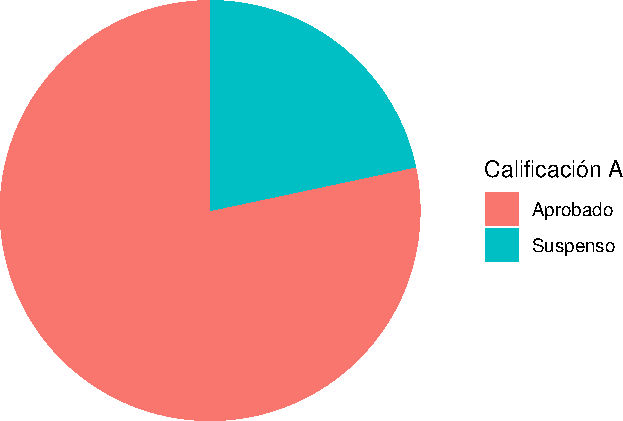
\includegraphics[keepaspectratio]{11-contrastes-una-poblacion_files/figure-pdf/unnamed-chunk-9-1.pdf}}

\begin{Shaded}
\begin{Highlighting}[]
\FunctionTok{ggplot}\NormalTok{(df, }\FunctionTok{aes}\NormalTok{(}\AttributeTok{x =}\NormalTok{ calificacionA)) }\SpecialCharTok{+}
  \FunctionTok{geom\_bar}\NormalTok{(}\AttributeTok{fill =} \StringTok{"steelblue"}\NormalTok{) }\SpecialCharTok{+}
  \FunctionTok{labs}\NormalTok{(}\AttributeTok{x =} \StringTok{"Calificación A"}\NormalTok{, }\AttributeTok{y =} \StringTok{"Número de alumnos"}\NormalTok{)}
\end{Highlighting}
\end{Shaded}

\pandocbounded{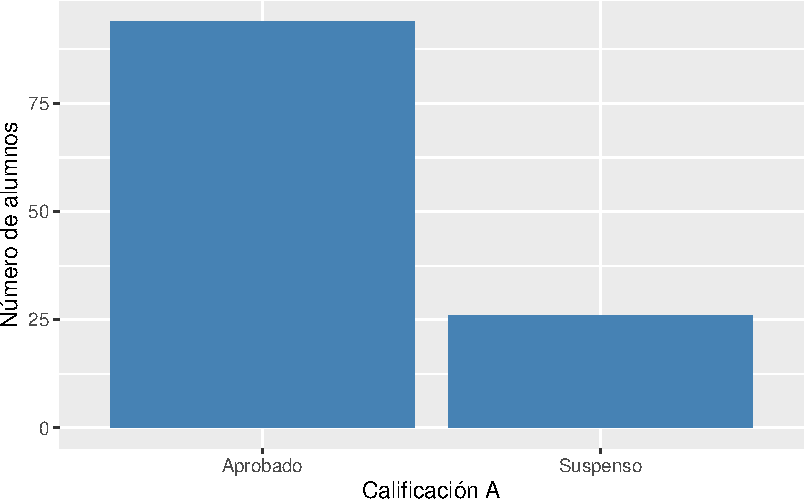
\includegraphics[keepaspectratio]{11-contrastes-una-poblacion_files/figure-pdf/unnamed-chunk-10-1.pdf}}

Los dos gráficos muestran la misma información (una amplia mayoría de
aprobados en la prueba A frente a una minoría de suspensos), pero el
diagrama de barras permite leer con más precisión el número de alumnos
de cada categoría.

\subsection{Test binomial para una
proporción}\label{test-binomial-para-una-proporciuxf3n}

\begin{definition}[Test binomial para una
proporción]\protect\hypertarget{def-unapoblacion-test-binomial-proporcion}{}\label{def-unapoblacion-test-binomial-proporcion}

El test binomial exacto permite contrastar si la proporción poblacional
de una de las dos categorías de una variable cualitativa dicotómica,
\(p\), es igual a un valor de referencia \(p_0\). La hipótesis nula es

\[H_0: p = p_0,\]

frente a una alternativa bilateral o unilateral, según el interés del
estudio. El contraste se basa directamente en la distribución binomial
exacta, sin recurrir a ninguna aproximación.

\end{definition}

\textbf{Requisitos}: variable cualitativa con exactamente dos
categorías. Al ser un contraste exacto, es válido para cualquier tamaño
muestral, incluidas las muestras pequeñas en las que no es aplicable la
aproximación normal.

Un objetivo habitual en la evaluación de un curso es comprobar si la
tasa de aprobados de una prueba supera un determinado umbral, por
ejemplo el 70\%. A continuación se contrasta si la proporción de
aprobados en \texttt{calificacionA} es superior a 0.7.

\begin{example}[]\protect\hypertarget{exm-unapoblacion-test-binomial-proporcion}{}\label{exm-unapoblacion-test-binomial-proporcion}

~

\begin{Shaded}
\begin{Highlighting}[]
\FunctionTok{binom.test}\NormalTok{(}\AttributeTok{x =} \FunctionTok{table}\NormalTok{(df}\SpecialCharTok{$}\NormalTok{calificacionA)[}\StringTok{"Aprobado"}\NormalTok{], }\AttributeTok{n =} \FunctionTok{nrow}\NormalTok{(df), }\AttributeTok{p =} \FloatTok{0.7}\NormalTok{,}
           \AttributeTok{alternative =} \StringTok{"greater"}\NormalTok{)}
\end{Highlighting}
\end{Shaded}

\begin{verbatim}

    Exact binomial test

data:  table(df$calificacionA)["Aprobado"] and nrow(df)
number of successes = 94, number of trials = 120, p-value = 0.02657
alternative hypothesis: true probability of success is greater than 0.7
95 percent confidence interval:
 0.7123183 1.0000000
sample estimates:
probability of success 
             0.7833333 
\end{verbatim}

De los 120 alumnos, 94 aprobaron la prueba A, una proporción muestral de
\(\hat{p}=0.783\). El p-valor del contraste es \(0.027\), inferior a
0.05, por lo que se rechaza \(H_0\): hay evidencia suficiente para
afirmar que la proporción real de aprobados en la prueba A es superior
al 70\%.

\end{example}

\subsection{Test Z para una
proporción}\label{test-z-para-una-proporciuxf3n}

\begin{definition}[Test Z para una
proporción]\protect\hypertarget{def-unapoblacion-test-z-proporcion}{}\label{def-unapoblacion-test-z-proporcion}

El test Z para una proporción persigue el mismo objetivo que el test
binomial (contrastar si una proporción poblacional \(p\) es igual a un
valor de referencia \(p_0\), con hipótesis nula \(H_0: p = p_0\)), pero
en lugar de usar la distribución binomial exacta se apoya en la
aproximación normal a la binomial, con corrección de continuidad.

\end{definition}

\textbf{Requisitos}: variable cualitativa con dos categorías y tamaño
muestral suficientemente grande (\(n \geq 30\), y en particular
\(np_0 \geq 5\) y \(n(1-p_0) \geq 5\)) para que la aproximación normal a
la binomial sea razonable. Con muestras pequeñas es preferible el test
binomial exacto.

El tamaño de la muestra de este curso, \(n=120\), es suficientemente
grande como para aplicar también el test Z sobre el mismo contraste de
la proporción de aprobados en \texttt{calificacionA}.

\begin{example}[]\protect\hypertarget{exm-unapoblacion-test-z-proporcion}{}\label{exm-unapoblacion-test-z-proporcion}

~

\begin{Shaded}
\begin{Highlighting}[]
\FunctionTok{prop.test}\NormalTok{(}\AttributeTok{x =} \FunctionTok{table}\NormalTok{(df}\SpecialCharTok{$}\NormalTok{calificacionA)[}\StringTok{"Aprobado"}\NormalTok{], }\AttributeTok{n =} \FunctionTok{nrow}\NormalTok{(df), }\AttributeTok{p =} \FloatTok{0.7}\NormalTok{,}
          \AttributeTok{alternative =} \StringTok{"greater"}\NormalTok{)}
\end{Highlighting}
\end{Shaded}

\begin{verbatim}

    1-sample proportions test with continuity correction

data:  table(df$calificacionA)["Aprobado"] out of nrow(df), null probability 0.7
X-squared = 3.5813, df = 1, p-value = 0.02922
alternative hypothesis: true p is greater than 0.7
95 percent confidence interval:
 0.7111099 1.0000000
sample estimates:
        p 
0.7833333 
\end{verbatim}

El estadístico de este contraste es \(\chi^2=3.58\) (equivalente a un
estadístico Z al cuadrado) con un p-valor de \(0.029\), también inferior
a 0.05. La conclusión coincide con la del test binomial exacto: se
rechaza \(H_0\) y se concluye que la proporción de aprobados en la
prueba A es significativamente superior al 70\%. El p-valor obtenido con
la aproximación normal (0.029) es muy similar al del test exacto
(0.027), como cabía esperar con un tamaño muestral de 120 alumnos,
aunque en muestras pequeñas ambos contrastes pueden diferir de forma más
apreciable.

\end{example}

\chapter{Contrastes para dos poblaciones
independientes}\label{contrastes-para-dos-poblaciones-independientes}

Este capítulo desarrolla la primera fila de la
\hyperref[selecciuxf3n-del-contraste-estaduxedstico-1]{tabla de
decisión} que involucra a dos variables: aquella en la que la variable
independiente es cualitativa con dos categorías, cada una
correspondiente a un grupo de individuos \textbf{distintos} (poblaciones
independientes), y se quiere contrastar si existen diferencias entre
esos dos grupos en una variable dependiente, ya sea esta cuantitativa o
cualitativa. Los ejemplos utilizan el conjunto de datos
\texttt{datos-curso.csv} presentado en el
\hyperref[selecciuxf3n-del-contraste-estaduxedstico-1]{capítulo
anterior}, comparando a los alumnos según su \texttt{sexo} (Hombre /
Mujer), dos grupos formados por alumnos diferentes y por tanto
independientes entre sí.

\section{Variable dependiente
cuantitativa}\label{variable-dependiente-cuantitativa}

Cuando la variable dependiente es cuantitativa, el objetivo habitual es
comparar la nota obtenida en la primera prueba, \texttt{notaA}, entre
los alumnos y las alumnas. Antes de aplicar ningún contraste conviene
describir y representar gráficamente los datos, y comprobar si es
razonable asumir que \texttt{notaA} sigue una distribución normal dentro
de cada grupo, ya que de ello depende qué contraste es el más apropiado.

\subsection{Estadísticos descriptivos por
grupo}\label{estaduxedsticos-descriptivos-por-grupo}

\begin{Shaded}
\begin{Highlighting}[]
\FunctionTok{library}\NormalTok{(moments)}

\NormalTok{df }\SpecialCharTok{\%\textgreater{}\%}
  \FunctionTok{group\_by}\NormalTok{(sexo) }\SpecialCharTok{\%\textgreater{}\%}
  \FunctionTok{summarise}\NormalTok{(}
    \AttributeTok{n =} \FunctionTok{n}\NormalTok{(),}
    \AttributeTok{media =} \FunctionTok{mean}\NormalTok{(notaA),}
    \AttributeTok{de =} \FunctionTok{sd}\NormalTok{(notaA),}
    \AttributeTok{minimo =} \FunctionTok{min}\NormalTok{(notaA),}
    \AttributeTok{Q1 =} \FunctionTok{quantile}\NormalTok{(notaA, }\FloatTok{0.25}\NormalTok{),}
    \AttributeTok{mediana =} \FunctionTok{median}\NormalTok{(notaA),}
    \AttributeTok{Q3 =} \FunctionTok{quantile}\NormalTok{(notaA, }\FloatTok{0.75}\NormalTok{),}
    \AttributeTok{maximo =} \FunctionTok{max}\NormalTok{(notaA),}
    \AttributeTok{asimetria =} \FunctionTok{skewness}\NormalTok{(notaA),}
    \AttributeTok{apuntamiento =} \FunctionTok{kurtosis}\NormalTok{(notaA)}
\NormalTok{  )}
\end{Highlighting}
\end{Shaded}

\begin{verbatim}
# A tibble: 2 x 11
  sexo       n media    de minimo    Q1 mediana    Q3 maximo asimetria
  <chr>  <int> <dbl> <dbl>  <dbl> <dbl>   <dbl> <dbl>  <dbl>     <dbl>
1 Hombre    71  6.12  1.23    3.5   5.3     6.1  6.85    9.3     0.249
2 Mujer     49  5.89  1.49    2.5   5       5.7  6.8     9.3     0.135
# i 1 more variable: apuntamiento <dbl>
\end{verbatim}

Los dos grupos tienen un tamaño razonable (71 hombres y 49 mujeres),
medias muy parecidas (6.12 frente a 5.89) y coeficientes de asimetría y
apuntamiento próximos a los valores 0 y 3 propios de la distribución
normal, lo que sugiere que ninguno de los dos grupos se aparta mucho de
la normalidad.

\subsection{Representación gráfica}\label{representaciuxf3n-gruxe1fica}

El diagrama de cajas y bigotes y el diagrama de violín permiten comparar
visualmente la posición, la dispersión y la forma de la distribución de
\texttt{notaA} en ambos grupos.

\begin{Shaded}
\begin{Highlighting}[]
\FunctionTok{ggplot}\NormalTok{(df, }\FunctionTok{aes}\NormalTok{(}\AttributeTok{x =}\NormalTok{ sexo, }\AttributeTok{y =}\NormalTok{ notaA, }\AttributeTok{fill =}\NormalTok{ sexo)) }\SpecialCharTok{+}
  \FunctionTok{geom\_boxplot}\NormalTok{() }\SpecialCharTok{+}
  \FunctionTok{scale\_fill\_brewer}\NormalTok{(}\AttributeTok{palette =} \StringTok{"Set2"}\NormalTok{) }\SpecialCharTok{+}
  \FunctionTok{labs}\NormalTok{(}\AttributeTok{x =} \StringTok{"Sexo"}\NormalTok{, }\AttributeTok{y =} \StringTok{"Nota A"}\NormalTok{) }\SpecialCharTok{+}
  \FunctionTok{theme\_minimal}\NormalTok{() }\SpecialCharTok{+}
  \FunctionTok{theme}\NormalTok{(}\AttributeTok{legend.position =} \StringTok{"none"}\NormalTok{)}
\end{Highlighting}
\end{Shaded}

\begin{figure}[H]

{\centering \pandocbounded{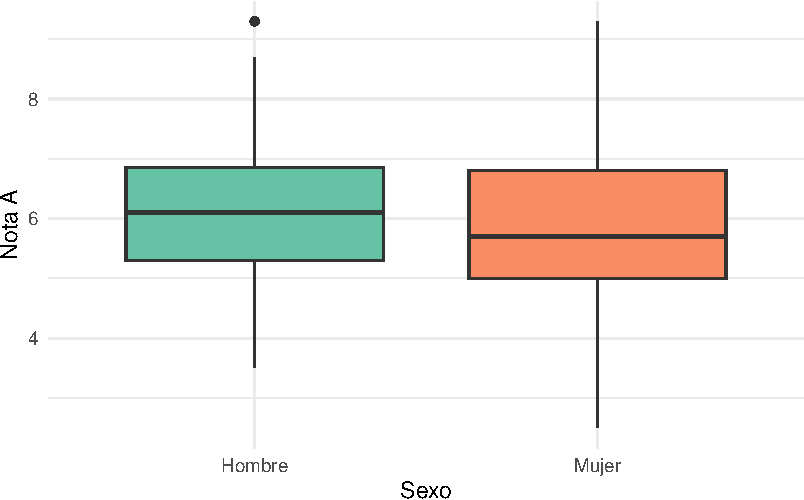
\includegraphics[keepaspectratio]{12-contrastes-dos-poblaciones-independientes_files/figure-pdf/boxplot-notaA-sexo-1.pdf}}

}

\caption{Diagrama de cajas y bigotes de la nota A según el sexo.}

\end{figure}%

\begin{Shaded}
\begin{Highlighting}[]
\FunctionTok{ggplot}\NormalTok{(df, }\FunctionTok{aes}\NormalTok{(}\AttributeTok{x =}\NormalTok{ sexo, }\AttributeTok{y =}\NormalTok{ notaA, }\AttributeTok{fill =}\NormalTok{ sexo)) }\SpecialCharTok{+}
  \FunctionTok{geom\_violin}\NormalTok{() }\SpecialCharTok{+}
  \FunctionTok{scale\_fill\_brewer}\NormalTok{(}\AttributeTok{palette =} \StringTok{"Set2"}\NormalTok{) }\SpecialCharTok{+}
  \FunctionTok{labs}\NormalTok{(}\AttributeTok{x =} \StringTok{"Sexo"}\NormalTok{, }\AttributeTok{y =} \StringTok{"Nota A"}\NormalTok{) }\SpecialCharTok{+}
  \FunctionTok{theme\_minimal}\NormalTok{() }\SpecialCharTok{+}
  \FunctionTok{theme}\NormalTok{(}\AttributeTok{legend.position =} \StringTok{"none"}\NormalTok{)}
\end{Highlighting}
\end{Shaded}

\begin{figure}[H]

{\centering \pandocbounded{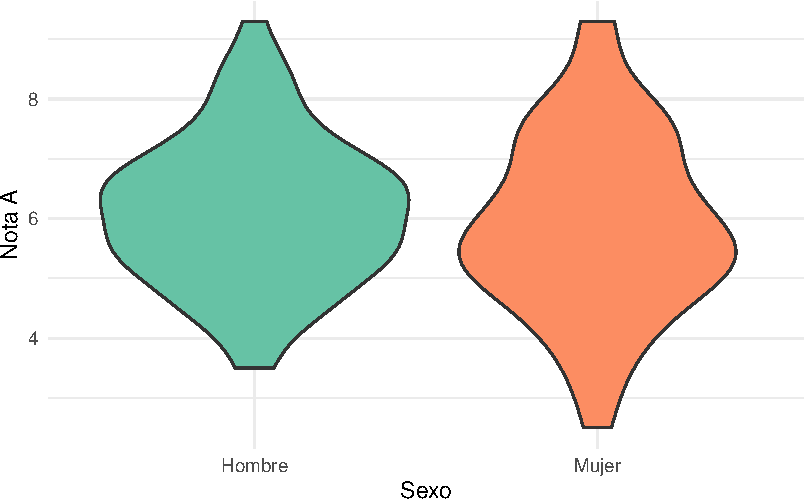
\includegraphics[keepaspectratio]{12-contrastes-dos-poblaciones-independientes_files/figure-pdf/violin-notaA-sexo-1.pdf}}

}

\caption{Diagrama de violín de la nota A según el sexo.}

\end{figure}%

Ambos gráficos muestran cajas y formas muy similares en los dos grupos,
sin apenas solapamiento asimétrico ni valores atípicos destacados, lo
que anticipa que es poco probable encontrar diferencias relevantes entre
ambos grupos.

\subsection{Comprobación de la
normalidad}\label{comprobaciuxf3n-de-la-normalidad}

Antes de decidir entre un contraste paramétrico (test t) o no
paramétrico (test U de Mann-Whitney) hay que comprobar la normalidad de
\texttt{notaA} \textbf{en cada grupo por separado}, con el test de
Shapiro-Wilk visto en el capítulo de
\hyperref[contrastes-para-una-poblaciuxf3n]{contrastes para una
población}:

\begin{Shaded}
\begin{Highlighting}[]
\NormalTok{df }\SpecialCharTok{\%\textgreater{}\%}
  \FunctionTok{group\_by}\NormalTok{(sexo) }\SpecialCharTok{\%\textgreater{}\%}
  \FunctionTok{summarise}\NormalTok{(}
    \AttributeTok{n =} \FunctionTok{n}\NormalTok{(),}
    \StringTok{\textasciigrave{}}\AttributeTok{p{-}valor}\StringTok{\textasciigrave{}} \OtherTok{=} \FunctionTok{shapiro.test}\NormalTok{(notaA)}\SpecialCharTok{$}\NormalTok{p.value}
\NormalTok{  )}
\end{Highlighting}
\end{Shaded}

\begin{verbatim}
# A tibble: 2 x 3
  sexo       n `p-valor`
  <chr>  <int>     <dbl>
1 Hombre    71     0.872
2 Mujer     49     0.942
\end{verbatim}

En ambos grupos el p-valor del test de Shapiro-Wilk es muy superior a
0.05 (0.872 en hombres y 0.942 en mujeres), por lo que no hay evidencia
para rechazar la normalidad de \texttt{notaA} en ninguno de los dos
grupos. Se cumple, por tanto, el requisito para aplicar los contrastes
paramétricos (test F y test t) que se muestran a continuación.

\subsection{Test F de Fisher de comparación de
varianzas}\label{test-f-de-fisher-de-comparaciuxf3n-de-varianzas}

\begin{definition}[Test F de Fisher de comparación de
varianzas]\protect\hypertarget{def-dosindep-test-f}{}\label{def-dosindep-test-f}

El \emph{test F de Fisher} contrasta si las varianzas de una variable
cuantitativa son iguales en dos poblaciones independientes. La hipótesis
nula es

\[H_0: \sigma_1^2 = \sigma_2^2\]

frente a la hipótesis alternativa \(H_1: \sigma_1^2 \neq \sigma_2^2\).

\end{definition}

\textbf{Requisitos}: la variable dependiente debe ser cuantitativa y
seguir una distribución normal en ambas poblaciones (o,
alternativamente, cada grupo debe tener un tamaño muestral
\(n \geq 30\)).

Comprobada la normalidad de \texttt{notaA} en ambos grupos, puede
aplicarse el test F para decidir si, a la hora de comparar las medias,
debe asumirse o no que las varianzas poblacionales son iguales.

\begin{example}[]\protect\hypertarget{exm-dosindep-test-f}{}\label{exm-dosindep-test-f}

~

\begin{Shaded}
\begin{Highlighting}[]
\FunctionTok{var.test}\NormalTok{(notaA }\SpecialCharTok{\textasciitilde{}}\NormalTok{ sexo, }\AttributeTok{data =}\NormalTok{ df)}
\end{Highlighting}
\end{Shaded}

\begin{verbatim}

    F test to compare two variances

data:  notaA by sexo
F = 0.6769, num df = 70, denom df = 48, p-value = 0.1347
alternative hypothesis: true ratio of variances is not equal to 1
95 percent confidence interval:
 0.3953421 1.1293155
sample estimates:
ratio of variances 
         0.6769032 
\end{verbatim}

El p-valor del contraste es 0.1347, superior a 0.05, por lo que no se
rechaza la hipótesis nula: no hay evidencia de que las varianzas de
\texttt{notaA} difieran entre hombres y mujeres, y puede asumirse la
igualdad de varianzas al aplicar el test t de comparación de medias.

\end{example}

\subsection{Test t de comparación de medias de poblaciones
independientes}\label{test-t-de-comparaciuxf3n-de-medias-de-poblaciones-independientes}

\begin{definition}[Test t de comparación de medias de poblaciones
independientes]\protect\hypertarget{def-dosindep-test-t}{}\label{def-dosindep-test-t}

El \emph{test t de comparación de medias de poblaciones independientes}
contrasta si las medias de una variable cuantitativa normal son iguales
en dos poblaciones independientes. La hipótesis nula es

\[H_0: \mu_1 = \mu_2\]

frente a la hipótesis alternativa \(H_1: \mu_1 \neq \mu_2\) (o una
alternativa unilateral, si procede).

\end{definition}

\textbf{Requisitos}: la variable dependiente debe ser cuantitativa y
seguir una distribución normal en ambas poblaciones (o cada grupo debe
tener \(n \geq 30\)). El cálculo del estadístico del contraste depende,
además, de si las varianzas poblacionales pueden considerarse iguales o
no, lo que se determina con el test F anterior: si las varianzas son
homogéneas se emplea la versión clásica del test t
(\texttt{var.equal\ =\ TRUE}); si no lo son, se emplea la corrección de
Welch (\texttt{var.equal\ =\ FALSE}), que es además la opción por
defecto en R y una elección razonable siempre que exista alguna duda
sobre la igualdad de varianzas.

Como el test F no ha encontrado diferencias significativas entre las
varianzas, cabría esperar que ambas versiones del test t den resultados
muy parecidos. Se aplica el test t con la corrección de Welch, más
conservadora y por tanto más segura como opción por defecto:

\begin{example}[]\protect\hypertarget{exm-dosindep-test-t}{}\label{exm-dosindep-test-t}

~

\begin{Shaded}
\begin{Highlighting}[]
\FunctionTok{t.test}\NormalTok{(notaA }\SpecialCharTok{\textasciitilde{}}\NormalTok{ sexo, }\AttributeTok{data =}\NormalTok{ df, }\AttributeTok{alternative =} \StringTok{"two.sided"}\NormalTok{, }\AttributeTok{var.equal =} \ConstantTok{FALSE}\NormalTok{)}
\end{Highlighting}
\end{Shaded}

\begin{verbatim}

    Welch Two Sample t-test

data:  notaA by sexo
t = 0.89364, df = 89.873, p-value = 0.3739
alternative hypothesis: true difference in means between group Hombre and group Mujer is not equal to 0
95 percent confidence interval:
 -0.2821809  0.7435779
sample estimates:
mean in group Hombre  mean in group Mujer 
            6.122535             5.891837 
\end{verbatim}

El p-valor es 0.3739, muy superior a 0.05, por lo que no se rechaza
\(H_0\): no hay evidencia de que la nota media de la primera prueba
difiera entre hombres y mujeres. Si se repite el contraste asumiendo
varianzas iguales (\texttt{var.equal\ =\ TRUE}), el resultado es
prácticamente idéntico (t = 0.926, p = 0.3563), como cabía esperar tras
el resultado del test F.

\end{example}

El siguiente diagrama de medias, con el intervalo de confianza al 95\%
de la media en cada grupo, ilustra gráficamente la conclusión del
contraste: los dos intervalos se solapan ampliamente, coherente con la
ausencia de diferencias significativas.

\begin{Shaded}
\begin{Highlighting}[]
\NormalTok{media\_ic }\OtherTok{\textless{}{-}} \ControlFlowTok{function}\NormalTok{(x) \{}
\NormalTok{  m }\OtherTok{\textless{}{-}} \FunctionTok{mean}\NormalTok{(x)}
\NormalTok{  error }\OtherTok{\textless{}{-}} \FunctionTok{qt}\NormalTok{(}\FloatTok{0.975}\NormalTok{, }\AttributeTok{df =} \FunctionTok{length}\NormalTok{(x) }\SpecialCharTok{{-}} \DecValTok{1}\NormalTok{) }\SpecialCharTok{*} \FunctionTok{sd}\NormalTok{(x) }\SpecialCharTok{/} \FunctionTok{sqrt}\NormalTok{(}\FunctionTok{length}\NormalTok{(x))}
  \FunctionTok{data.frame}\NormalTok{(}\AttributeTok{y =}\NormalTok{ m, }\AttributeTok{ymin =}\NormalTok{ m }\SpecialCharTok{{-}}\NormalTok{ error, }\AttributeTok{ymax =}\NormalTok{ m }\SpecialCharTok{+}\NormalTok{ error)}
\NormalTok{\}}

\FunctionTok{ggplot}\NormalTok{(df, }\FunctionTok{aes}\NormalTok{(}\AttributeTok{x =}\NormalTok{ sexo, }\AttributeTok{y =}\NormalTok{ notaA, }\AttributeTok{color =}\NormalTok{ sexo)) }\SpecialCharTok{+}
  \FunctionTok{stat\_summary}\NormalTok{(}\AttributeTok{fun =} \StringTok{"mean"}\NormalTok{, }\AttributeTok{geom =} \StringTok{"point"}\NormalTok{, }\AttributeTok{size =} \DecValTok{3}\NormalTok{) }\SpecialCharTok{+}
  \FunctionTok{stat\_summary}\NormalTok{(}\AttributeTok{fun.data =}\NormalTok{ media\_ic, }\AttributeTok{geom =} \StringTok{"pointrange"}\NormalTok{) }\SpecialCharTok{+}
  \FunctionTok{labs}\NormalTok{(}\AttributeTok{x =} \StringTok{"Sexo"}\NormalTok{, }\AttributeTok{y =} \StringTok{"Nota A media"}\NormalTok{) }\SpecialCharTok{+}
  \FunctionTok{theme\_minimal}\NormalTok{() }\SpecialCharTok{+}
  \FunctionTok{theme}\NormalTok{(}\AttributeTok{legend.position =} \StringTok{"none"}\NormalTok{)}
\end{Highlighting}
\end{Shaded}

\begin{figure}[H]

{\centering \pandocbounded{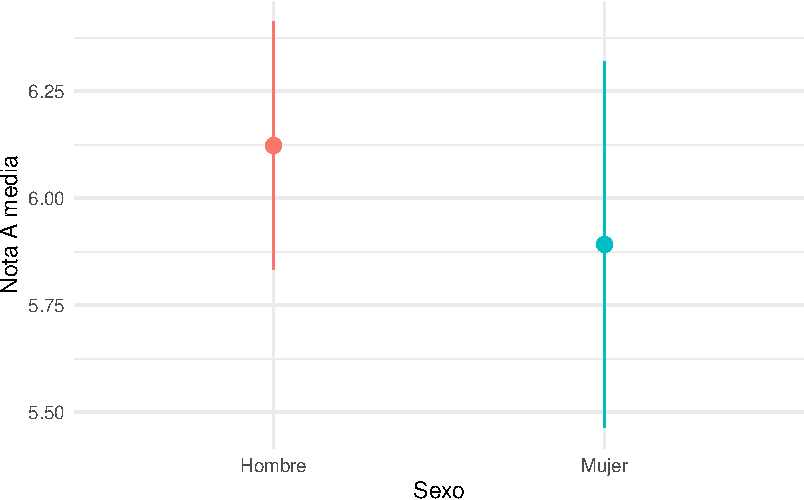
\includegraphics[keepaspectratio]{12-contrastes-dos-poblaciones-independientes_files/figure-pdf/diagrama-medias-notaA-sexo-1.pdf}}

}

\caption{Media de la nota A por sexo, con su intervalo de confianza al
95\%.}

\end{figure}%

\subsection{Test U de Mann-Whitney}\label{test-u-de-mann-whitney}

\begin{definition}[Test U de
Mann-Whitney]\protect\hypertarget{def-dosindep-test-u-mann-whitney}{}\label{def-dosindep-test-u-mann-whitney}

El \emph{test U de Mann-Whitney} (también llamado test de la suma de
rangos de Wilcoxon) contrasta si las distribuciones de una variable
cuantitativa o cualitativa ordinal son iguales en dos poblaciones
independientes, sin necesidad de asumir normalidad. Cuando las dos
distribuciones tienen la misma forma y dispersión, el contraste equivale
a comparar sus medianas. La hipótesis nula es

\[H_0: \mbox{las distribuciones de las dos poblaciones son iguales}\]

frente a la alternativa de que una de las poblaciones tiende a presentar
valores sistemáticamente más altos (o más bajos) que la otra.

\end{definition}

\textbf{Requisitos}: la variable dependiente debe ser, al menos,
cualitativa ordinal (o cuantitativa), y las dos poblaciones deben ser
independientes. No exige que la variable siga una distribución normal,
por lo que es la alternativa natural al test t cuando no se cumple ese
requisito.

Aunque en este caso \texttt{notaA} es normal en ambos grupos y el test t
es aplicable, se muestra también el test U de Mann-Whitney a modo
ilustrativo, ya que sería la opción adecuada si la normalidad no se
hubiera cumplido:

\begin{example}[]\protect\hypertarget{exm-dosindep-test-u-mann-whitney}{}\label{exm-dosindep-test-u-mann-whitney}

~

\begin{Shaded}
\begin{Highlighting}[]
\FunctionTok{wilcox.test}\NormalTok{(notaA }\SpecialCharTok{\textasciitilde{}}\NormalTok{ sexo, }\AttributeTok{data =}\NormalTok{ df, }\AttributeTok{alternative =} \StringTok{"two.sided"}\NormalTok{)}
\end{Highlighting}
\end{Shaded}

\begin{verbatim}

    Wilcoxon rank sum test with continuity correction

data:  notaA by sexo
W = 1917, p-value = 0.3445
alternative hypothesis: true location shift is not equal to 0
\end{verbatim}

El p-valor es 0.3445, superior a 0.05, por lo que tampoco con este
contraste no paramétrico se rechaza la hipótesis nula: la distribución
de \texttt{notaA} no difiere significativamente entre hombres y mujeres,
confirmando la conclusión alcanzada con el test t.

\end{example}

\section{Variable dependiente
cualitativa}\label{variable-dependiente-cualitativa}

Cuando la variable dependiente es cualitativa, el interés no está en
comparar medias sino en comparar \textbf{proporciones}, o, de forma
equivalente, en contrastar si existe \textbf{asociación} entre las dos
variables cualitativas. Como ejemplo se compara el resultado (Aprobado /
Suspenso) de la primera prueba, \texttt{calificacionA}, entre hombres y
mujeres.

La tabla de contingencia entre \texttt{sexo} y \texttt{calificacionA}, y
las proporciones de aprobados dentro de cada sexo, son las siguientes:

\begin{Shaded}
\begin{Highlighting}[]
\NormalTok{tabla }\OtherTok{\textless{}{-}} \FunctionTok{table}\NormalTok{(df}\SpecialCharTok{$}\NormalTok{sexo, df}\SpecialCharTok{$}\NormalTok{calificacionA)}
\NormalTok{tabla}
\end{Highlighting}
\end{Shaded}

\begin{verbatim}
        
         Aprobado Suspenso
  Hombre       58       13
  Mujer        36       13
\end{verbatim}

\begin{Shaded}
\begin{Highlighting}[]
\FunctionTok{prop.table}\NormalTok{(tabla, }\AttributeTok{margin =} \DecValTok{1}\NormalTok{)}
\end{Highlighting}
\end{Shaded}

\begin{verbatim}
        
          Aprobado  Suspenso
  Hombre 0.8169014 0.1830986
  Mujer  0.7346939 0.2653061
\end{verbatim}

El 81.7\% de los hombres aprueba la primera prueba, frente al 73.5\% de
las mujeres. La pregunta que responden los contrastes de esta sección es
si esa diferencia de casi 8 puntos porcentuales es lo bastante grande
como para no poder explicarse por el azar del muestreo, o si, por el
contrario, es compatible con que en la población no exista ninguna
diferencia real entre sexos.

\subsection{Test Chi-cuadrado de
independencia}\label{test-chi-cuadrado-de-independencia}

\begin{definition}[Test Chi-cuadrado de
independencia]\protect\hypertarget{def-dosindep-test-chi-cuadrado}{}\label{def-dosindep-test-chi-cuadrado}

El \emph{test Chi-cuadrado de independencia} contrasta si existe
relación (asociación) entre dos variables cualitativas, o, de forma
equivalente cuando una de ellas define dos poblaciones, si las
proporciones de las categorías de la otra variable son iguales en ambas
poblaciones. La hipótesis nula es

\[H_0: \mbox{las dos variables son independientes (no hay asociación entre ellas)}\]

\end{definition}

\textbf{Requisitos}: las dos variables deben ser cualitativas, y no más
del 20\% de las frecuencias esperadas de la tabla de contingencia debe
ser inferior a 5 (ninguna frecuencia esperada debe ser, además, inferior
a 1).

\begin{example}[]\protect\hypertarget{exm-dosindep-test-chi-cuadrado}{}\label{exm-dosindep-test-chi-cuadrado}

~

\begin{Shaded}
\begin{Highlighting}[]
\NormalTok{chi }\OtherTok{\textless{}{-}} \FunctionTok{chisq.test}\NormalTok{(tabla)}
\NormalTok{chi}
\end{Highlighting}
\end{Shaded}

\begin{verbatim}

    Pearson's Chi-squared test with Yates' continuity correction

data:  tabla
X-squared = 0.72085, df = 1, p-value = 0.3959
\end{verbatim}

\begin{Shaded}
\begin{Highlighting}[]
\NormalTok{chi}\SpecialCharTok{$}\NormalTok{expected}
\end{Highlighting}
\end{Shaded}

\begin{verbatim}
        
         Aprobado Suspenso
  Hombre 55.61667 15.38333
  Mujer  38.38333 10.61667
\end{verbatim}

Las cuatro frecuencias esperadas de la tabla (55.6, 15.4, 38.4 y 10.6)
son todas superiores a 5, por lo que se cumple el requisito de
aplicación del test. El p-valor obtenido, con la corrección de
continuidad de Yates propia de las tablas 2x2, es 0.3959, muy superior a
0.05, por lo que no se rechaza la hipótesis nula: no hay evidencia de
asociación entre el sexo y el resultado de la primera prueba, es decir,
la proporción de aprobados no difiere significativamente entre hombres y
mujeres.

\end{example}

\subsection{Test exacto de Fisher}\label{test-exacto-de-fisher}

\begin{definition}[Test exacto de
Fisher]\protect\hypertarget{def-dosindep-test-fisher}{}\label{def-dosindep-test-fisher}

El \emph{test exacto de Fisher} contrasta la misma hipótesis de
independencia que el test Chi-cuadrado, pero calculando de forma exacta
(sin aproximación asintótica) la probabilidad de las tablas de
contingencia al menos tan extremas como la observada. La hipótesis nula
es la misma que la del test Chi-cuadrado:

\[H_0: \mbox{las dos variables son independientes (no hay asociación entre ellas)}\]

Es la alternativa recomendada, especialmente en tablas 2x2, cuando no se
cumple el requisito de frecuencias esperadas del test Chi-cuadrado
(muestras pequeñas).

\end{definition}

\textbf{Requisitos}: las dos variables deben ser cualitativas. A
diferencia del test Chi-cuadrado, no exige ninguna condición sobre las
frecuencias esperadas, por lo que es válido con cualquier tamaño
muestral.

\begin{example}[]\protect\hypertarget{exm-dosindep-test-fisher}{}\label{exm-dosindep-test-fisher}

~

\begin{Shaded}
\begin{Highlighting}[]
\FunctionTok{fisher.test}\NormalTok{(tabla)}
\end{Highlighting}
\end{Shaded}

\begin{verbatim}

    Fisher's Exact Test for Count Data

data:  tabla
p-value = 0.3677
alternative hypothesis: true odds ratio is not equal to 1
95 percent confidence interval:
 0.609684 4.234633
sample estimates:
odds ratio 
  1.604498 
\end{verbatim}

El p-valor del test exacto de Fisher es 0.3677, muy similar al obtenido
con el test Chi-cuadrado (0.3959) y, de nuevo, muy superior a 0.05: no
se rechaza la hipótesis nula de independencia. Este parecido entre ambos
resultados es el esperable, ya que las frecuencias esperadas de la tabla
de contingencia eran, como se comprobó antes, suficientemente grandes
para que el test Chi-cuadrado fuera fiable; el test exacto de Fisher
habría sido la opción obligada, en cambio, de haber tenido frecuencias
esperadas por debajo de 5.

\end{example}

\section{Resumen}\label{resumen}

En los cinco contrastes de este capítulo, ninguno ha encontrado
diferencias estadísticamente significativas entre hombres y mujeres, ni
en la nota media de la primera prueba ni en la proporción de aprobados,
lo que es coherente con lo observado en las descriptivas y los gráficos
iniciales: los dos grupos se comportan, en esta asignatura, de forma muy
similar.

Todos los contrastes anteriores exigen que las dos poblaciones
comparadas estén formadas por individuos distintos, es decir, que sean
independientes. Cuando en cambio se comparan los mismos individuos
medidos en dos ocasiones (por ejemplo, la nota de un mismo alumno en dos
pruebas distintas, \texttt{notaA} y \texttt{notaB}), las poblaciones
están pareadas y los contrastes anteriores dejan de ser válidos, siendo
necesario recurrir a sus versiones para datos pareados, que se
desarrollan en el capítulo de
\href{13-contrastes-dos-poblaciones-pareadas.qmd}{Contrastes para dos
poblaciones pareadas}. Y cuando la variable independiente tiene más de
dos categorías (por ejemplo, comparar la nota media entre los tres
grupos de clase, A, B y C), es necesario recurrir a los contrastes que
se desarrollan en el capítulo de
\href{14-contrastes-mas-dos-poblaciones-independientes.qmd}{Contrastes
para más de dos poblaciones independientes}.

\chapter{Contrastes para dos poblaciones
pareadas}\label{contrastes-para-dos-poblaciones-pareadas}

En el \hyperref[contrastes-para-dos-poblaciones-independientes]{capítulo
anterior} las dos poblaciones comparadas estaban formadas por individuos
distintos: por ejemplo, un grupo de hombres y un grupo de mujeres, sin
ninguna relación entre las observaciones de un grupo y las del otro. Sin
embargo, en muchos estudios las dos poblaciones que se comparan no son
independientes, sino que están \textbf{pareadas} o
\textbf{relacionadas}: los mismos individuos se miden dos veces, por
ejemplo antes y después de una intervención, o en dos condiciones,
momentos o pruebas distintas. En ese caso cada individuo aporta un
\textbf{par de valores relacionados entre sí}, y esa relación debe
tenerse en cuenta al elegir el contraste, porque ignorarla (tratando los
datos como si procedieran de dos grupos independientes) desaprovecha
información y puede llevar a conclusiones erróneas.

En el conjunto de datos del curso, \texttt{notaA} y \texttt{notaB} son
las calificaciones obtenidas por los mismos 120 alumnos en dos
asignaturas distintas, por lo que cada alumno aporta un par de notas
relacionadas entre sí (un alumno con buen rendimiento tenderá a obtener
buenas notas en ambas asignaturas). Lo mismo ocurre con
\texttt{calificacionA} y \texttt{calificacionB}, la versión cualitativa
(Aprobado / Suspenso) de esas mismas dos calificaciones. Este capítulo
presenta los contrastes adecuados para este tipo de comparaciones,
distinguiendo según si la variable dependiente es cuantitativa o
cualitativa.

\section{\texorpdfstring{Variable dependiente cuantitativa: comparar
\texttt{notaA} con
\texttt{notaB}}{Variable dependiente cuantitativa: comparar notaA con notaB}}\label{variable-dependiente-cuantitativa-comparar-notaa-con-notab}

Antes de plantear ningún contraste conviene visualizar la relación entre
las dos notas de cada alumno, precisamente para comprobar que están
pareadas y no son dos muestras independientes.

\begin{Shaded}
\begin{Highlighting}[]
\FunctionTok{ggplot}\NormalTok{(df, }\FunctionTok{aes}\NormalTok{(}\AttributeTok{x =}\NormalTok{ notaA, }\AttributeTok{y =}\NormalTok{ notaB)) }\SpecialCharTok{+}
  \FunctionTok{geom\_point}\NormalTok{(}\AttributeTok{alpha =} \FloatTok{0.6}\NormalTok{, }\AttributeTok{color =} \StringTok{"steelblue"}\NormalTok{) }\SpecialCharTok{+}
  \FunctionTok{geom\_abline}\NormalTok{(}\AttributeTok{slope =} \DecValTok{1}\NormalTok{, }\AttributeTok{intercept =} \DecValTok{0}\NormalTok{, }\AttributeTok{linetype =} \StringTok{"dashed"}\NormalTok{, }\AttributeTok{color =} \StringTok{"darkred"}\NormalTok{) }\SpecialCharTok{+}
  \FunctionTok{labs}\NormalTok{(}
    \AttributeTok{title =} \StringTok{"Nota de la asignatura A frente a la nota de la asignatura B"}\NormalTok{,}
    \AttributeTok{subtitle =} \StringTok{"por alumno; la línea discontinua marca la igualdad notaA = notaB"}\NormalTok{,}
    \AttributeTok{x =} \StringTok{"notaA"}\NormalTok{,}
    \AttributeTok{y =} \StringTok{"notaB"}
\NormalTok{  ) }\SpecialCharTok{+}
  \FunctionTok{theme\_minimal}\NormalTok{()}
\end{Highlighting}
\end{Shaded}

\pandocbounded{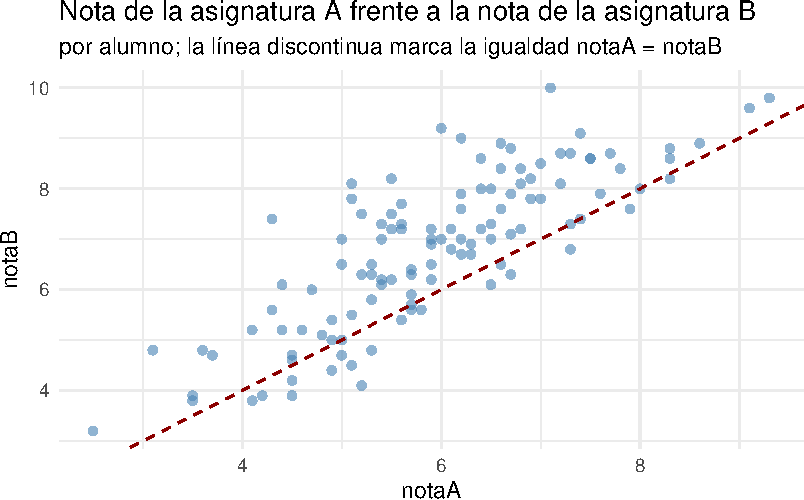
\includegraphics[keepaspectratio]{13-contrastes-dos-poblaciones-pareadas_files/figure-pdf/unnamed-chunk-1-1.pdf}}

\begin{Shaded}
\begin{Highlighting}[]
\FunctionTok{cor}\NormalTok{(df}\SpecialCharTok{$}\NormalTok{notaA, df}\SpecialCharTok{$}\NormalTok{notaB, }\AttributeTok{use =} \StringTok{"complete.obs"}\NormalTok{)}
\end{Highlighting}
\end{Shaded}

\begin{verbatim}
[1] 0.8104926
\end{verbatim}

La correlación entre \texttt{notaA} y \texttt{notaB} es de 0.81: un
alumno con una nota alta en la asignatura A tiende a tener también una
nota alta en la B, lo que confirma que ambas notas están relacionadas y
proceden de los mismos individuos, y no de dos grupos de alumnos
distintos. En el diagrama de dispersión se observa además que la mayoría
de los puntos quedan por debajo de la línea discontinua
\texttt{notaA\ =\ notaB} (92 de los 115 alumnos con ambas notas), es
decir, que la mayoría de los alumnos obtiene una nota más alta en B que
en A. Precisamente por existir esta relación entre las dos mediciones,
el contraste debe tener en cuenta el emparejamiento en lugar de tratar
\texttt{notaA} y \texttt{notaB} como si procedieran de dos poblaciones
independientes.

Para comparar las notas de la asignatura A y de la asignatura B de los
mismos alumnos conviene empezar creando la variable que resume, para
cada alumno, la diferencia entre ambas notas:

\begin{Shaded}
\begin{Highlighting}[]
\NormalTok{df }\OtherTok{\textless{}{-}}\NormalTok{ df }\SpecialCharTok{\%\textgreater{}\%} \FunctionTok{mutate}\NormalTok{(}\AttributeTok{diferencia\_AB =}\NormalTok{ notaA }\SpecialCharTok{{-}}\NormalTok{ notaB)}
\end{Highlighting}
\end{Shaded}

Esta variable \texttt{diferencia\_AB} es la clave de todo este apartado:
un contraste sobre dos poblaciones pareadas puede plantearse de forma
equivalente como un contraste sobre esta única variable diferencia
frente al valor 0, exactamente igual que los contrastes sobre la media o
la mediana de una sola población que se vieron en el capítulo de
\hyperref[contrastes-para-una-poblaciuxf3n]{contrastes para una
población}. Si no hay diferencia real entre las dos asignaturas, la
diferencia \texttt{diferencia\_AB} debería distribuirse en torno a 0; si
una de las dos asignaturas tiende a puntuar más alto que la otra, la
diferencia se desplazará sistemáticamente por encima o por debajo de 0.

Cabe señalar que cinco alumnos no tienen registrada la nota de la
asignatura B (son valores perdidos, \texttt{NA}), por lo que la
diferencia también queda como \texttt{NA} en esos cinco casos. Todos los
análisis siguientes se basan, por tanto, en los 115 alumnos con datos
completos en ambas asignaturas.

\textbf{Estadísticos descriptivos de la diferencia}

\begin{Shaded}
\begin{Highlighting}[]
\FunctionTok{library}\NormalTok{(moments)}

\NormalTok{df }\SpecialCharTok{\%\textgreater{}\%}
  \FunctionTok{summarise}\NormalTok{(}
    \AttributeTok{n =} \FunctionTok{sum}\NormalTok{(}\SpecialCharTok{!}\FunctionTok{is.na}\NormalTok{(diferencia\_AB)),}
    \AttributeTok{media =} \FunctionTok{mean}\NormalTok{(diferencia\_AB, }\AttributeTok{na.rm =} \ConstantTok{TRUE}\NormalTok{),}
    \AttributeTok{dt =} \FunctionTok{sd}\NormalTok{(diferencia\_AB, }\AttributeTok{na.rm =} \ConstantTok{TRUE}\NormalTok{),}
    \AttributeTok{minimo =} \FunctionTok{min}\NormalTok{(diferencia\_AB, }\AttributeTok{na.rm =} \ConstantTok{TRUE}\NormalTok{),}
    \AttributeTok{Q1 =} \FunctionTok{quantile}\NormalTok{(diferencia\_AB, }\FloatTok{0.25}\NormalTok{, }\AttributeTok{na.rm =} \ConstantTok{TRUE}\NormalTok{),}
    \AttributeTok{mediana =} \FunctionTok{median}\NormalTok{(diferencia\_AB, }\AttributeTok{na.rm =} \ConstantTok{TRUE}\NormalTok{),}
    \AttributeTok{Q3 =} \FunctionTok{quantile}\NormalTok{(diferencia\_AB, }\FloatTok{0.75}\NormalTok{, }\AttributeTok{na.rm =} \ConstantTok{TRUE}\NormalTok{),}
    \AttributeTok{maximo =} \FunctionTok{max}\NormalTok{(diferencia\_AB, }\AttributeTok{na.rm =} \ConstantTok{TRUE}\NormalTok{),}
    \AttributeTok{asimetria =} \FunctionTok{skewness}\NormalTok{(diferencia\_AB, }\AttributeTok{na.rm =} \ConstantTok{TRUE}\NormalTok{),}
    \AttributeTok{apuntamiento =} \FunctionTok{kurtosis}\NormalTok{(diferencia\_AB, }\AttributeTok{na.rm =} \ConstantTok{TRUE}\NormalTok{)}
\NormalTok{  )}
\end{Highlighting}
\end{Shaded}

\begin{verbatim}
# A tibble: 1 x 10
      n  media    dt minimo    Q1 mediana     Q3 maximo asimetria apuntamiento
  <int>  <dbl> <dbl>  <dbl> <dbl>   <dbl>  <dbl>  <dbl>     <dbl>        <dbl>
1   115 -0.882 0.900   -3.2  -1.5    -0.8 -0.300   1.10    -0.430         2.86
\end{verbatim}

Sobre los 115 alumnos con ambas notas, la diferencia
\texttt{notaA\ -\ notaB} tiene una media de -0.88 y una desviación
típica de 0.90, con un mínimo de -3.2 y un máximo de 1.1 (cuartiles
-1.5, -0.8 y -0.3). El hecho de que la media y la mediana sean negativas
indica que, en general, los alumnos obtienen una nota más alta en la
asignatura B que en la A. El coeficiente de asimetría, -0.43, muestra
una ligera asimetría negativa (cola algo más larga hacia valores muy
negativos), y el apuntamiento, 2.86, es muy próximo a 3, el valor de
referencia de la distribución normal, lo que no sugiere colas
especialmente pesadas ni ligeras.

\textbf{Gráficos}

\begin{Shaded}
\begin{Highlighting}[]
\FunctionTok{ggplot}\NormalTok{(df, }\FunctionTok{aes}\NormalTok{(}\AttributeTok{y =}\NormalTok{ diferencia\_AB)) }\SpecialCharTok{+}
  \FunctionTok{geom\_boxplot}\NormalTok{(}\AttributeTok{fill =} \StringTok{"steelblue"}\NormalTok{, }\AttributeTok{alpha =} \FloatTok{0.6}\NormalTok{) }\SpecialCharTok{+}
  \FunctionTok{labs}\NormalTok{(}
    \AttributeTok{title =} \StringTok{"Diagrama de caja y bigotes de la diferencia notaA {-} notaB"}\NormalTok{,}
    \AttributeTok{y =} \StringTok{"Diferencia (notaA {-} notaB)"}
\NormalTok{  ) }\SpecialCharTok{+}
  \FunctionTok{theme\_minimal}\NormalTok{()}
\end{Highlighting}
\end{Shaded}

\pandocbounded{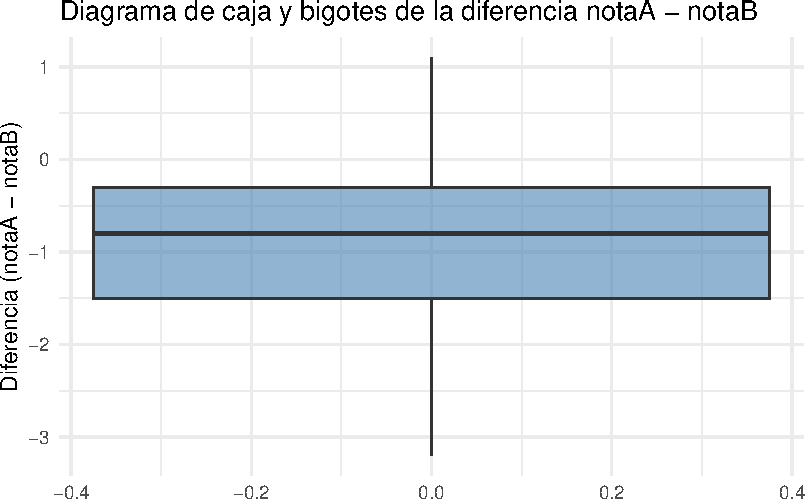
\includegraphics[keepaspectratio]{13-contrastes-dos-poblaciones-pareadas_files/figure-pdf/unnamed-chunk-5-1.pdf}}

El diagrama de caja confirma lo observado en los estadísticos
descriptivos: la caja se sitúa casi por completo por debajo de 0, sin
valores atípicos, lo que refuerza la idea de que la mayoría de los
alumnos sacan mejor nota en la asignatura B que en la A.

\textbf{Test de normalidad de Shapiro-Wilk sobre la diferencia}

\begin{Shaded}
\begin{Highlighting}[]
\FunctionTok{shapiro.test}\NormalTok{(df}\SpecialCharTok{$}\NormalTok{diferencia\_AB)}
\end{Highlighting}
\end{Shaded}

\begin{verbatim}

    Shapiro-Wilk normality test

data:  df$diferencia_AB
W = 0.9794, p-value = 0.07367
\end{verbatim}

El test de Shapiro-Wilk proporciona un p-valor de 0.074, mayor que 0.05,
por lo que no se rechaza la hipótesis nula de normalidad: puede asumirse
que la diferencia \texttt{diferencia\_AB} sigue una distribución
aproximadamente normal. Este resultado, junto con el hecho de disponer
de \(n=115\) pares (muy por encima de 30), respalda el uso del test t
para datos pareados que se presenta a continuación.

\subsection{Test t para datos
pareados}\label{test-t-para-datos-pareados}

\begin{definition}[Test t para datos
pareados]\protect\hypertarget{def-dospareadas-t-pareado}{}\label{def-dospareadas-t-pareado}

El \emph{test t para datos pareados} contrasta si existe diferencia
entre las medias de dos poblaciones pareadas, es decir, medidas sobre
los mismos individuos. Si \(D\) es la variable que recoge, para cada
individuo, la diferencia entre sus dos mediciones, y \(\mu_D\) es la
media poblacional de esa diferencia, el contraste plantea las hipótesis

\[H_0: \mu_D = 0 \quad \text{frente a} \quad H_1: \mu_D \neq 0,\]

siendo \(H_0\) equivalente a afirmar que las medias de las dos
poblaciones pareadas, \(\mu_1\) y \(\mu_2\), coinciden.

\end{definition}

\textbf{Requisitos}:

\begin{itemize}
\tightlist
\item
  La variable dependiente es cuantitativa y se mide dos veces sobre los
  mismos individuos (o sobre pares de individuos emparejados según algún
  criterio).
\item
  La variable diferencia \(D\) sigue una distribución normal, o bien el
  tamaño muestral es suficientemente grande (\(n \geq 30\)) para que el
  teorema central del límite garantice la normalidad aproximada de la
  media de las diferencias.
\end{itemize}

En el ejemplo, la diferencia \texttt{diferencia\_AB} no se ha podido
rechazar como normal (Shapiro-Wilk, \(p=0.074\)) y además se dispone de
\(n=115\) pares, por lo que se cumplen ambos requisitos y puede
aplicarse con garantías el test t para datos pareados para comparar las
notas medias de los mismos alumnos en las asignaturas A y B.

\begin{example}[]\protect\hypertarget{exm-dospareadas-t-pareado}{}\label{exm-dospareadas-t-pareado}

~

\begin{Shaded}
\begin{Highlighting}[]
\FunctionTok{t.test}\NormalTok{(df}\SpecialCharTok{$}\NormalTok{notaA, df}\SpecialCharTok{$}\NormalTok{notaB, }\AttributeTok{alternative =} \StringTok{"two.sided"}\NormalTok{, }\AttributeTok{paired =} \ConstantTok{TRUE}\NormalTok{)}
\end{Highlighting}
\end{Shaded}

\begin{verbatim}

    Paired t-test

data:  df$notaA and df$notaB
t = -10.506, df = 114, p-value < 2.2e-16
alternative hypothesis: true mean difference is not equal to 0
95 percent confidence interval:
 -1.048005 -0.715473
sample estimates:
mean difference 
     -0.8817391 
\end{verbatim}

\begin{Shaded}
\begin{Highlighting}[]
\NormalTok{media\_ic }\OtherTok{\textless{}{-}} \ControlFlowTok{function}\NormalTok{(x) \{}
\NormalTok{  x }\OtherTok{\textless{}{-}}\NormalTok{ x[}\SpecialCharTok{!}\FunctionTok{is.na}\NormalTok{(x)]}
\NormalTok{  m }\OtherTok{\textless{}{-}} \FunctionTok{mean}\NormalTok{(x)}
\NormalTok{  ee }\OtherTok{\textless{}{-}} \FunctionTok{sd}\NormalTok{(x) }\SpecialCharTok{/} \FunctionTok{sqrt}\NormalTok{(}\FunctionTok{length}\NormalTok{(x))}
\NormalTok{  ic }\OtherTok{\textless{}{-}} \FunctionTok{qt}\NormalTok{(}\FloatTok{0.975}\NormalTok{, }\AttributeTok{df =} \FunctionTok{length}\NormalTok{(x) }\SpecialCharTok{{-}} \DecValTok{1}\NormalTok{) }\SpecialCharTok{*}\NormalTok{ ee}
  \FunctionTok{data.frame}\NormalTok{(}\AttributeTok{y =}\NormalTok{ m, }\AttributeTok{ymin =}\NormalTok{ m }\SpecialCharTok{{-}}\NormalTok{ ic, }\AttributeTok{ymax =}\NormalTok{ m }\SpecialCharTok{+}\NormalTok{ ic)}
\NormalTok{\}}

\FunctionTok{ggplot}\NormalTok{(df, }\FunctionTok{aes}\NormalTok{(}\AttributeTok{x =} \StringTok{""}\NormalTok{, }\AttributeTok{y =}\NormalTok{ diferencia\_AB)) }\SpecialCharTok{+}
  \FunctionTok{stat\_summary}\NormalTok{(}\AttributeTok{fun.data =}\NormalTok{ media\_ic, }\AttributeTok{geom =} \StringTok{"errorbar"}\NormalTok{, }\AttributeTok{width =} \FloatTok{0.2}\NormalTok{, }\AttributeTok{color =} \StringTok{"darkred"}\NormalTok{) }\SpecialCharTok{+}
  \FunctionTok{stat\_summary}\NormalTok{(}\AttributeTok{fun =}\NormalTok{ mean, }\AttributeTok{geom =} \StringTok{"point"}\NormalTok{, }\AttributeTok{size =} \DecValTok{3}\NormalTok{, }\AttributeTok{color =} \StringTok{"darkred"}\NormalTok{) }\SpecialCharTok{+}
  \FunctionTok{labs}\NormalTok{(}
    \AttributeTok{title =} \StringTok{"Media e intervalo de confianza al 95\% de la diferencia notaA {-} notaB"}\NormalTok{,}
    \AttributeTok{x =} \ConstantTok{NULL}\NormalTok{,}
    \AttributeTok{y =} \StringTok{"Diferencia (notaA {-} notaB)"}
\NormalTok{  ) }\SpecialCharTok{+}
  \FunctionTok{theme\_minimal}\NormalTok{()}
\end{Highlighting}
\end{Shaded}

\pandocbounded{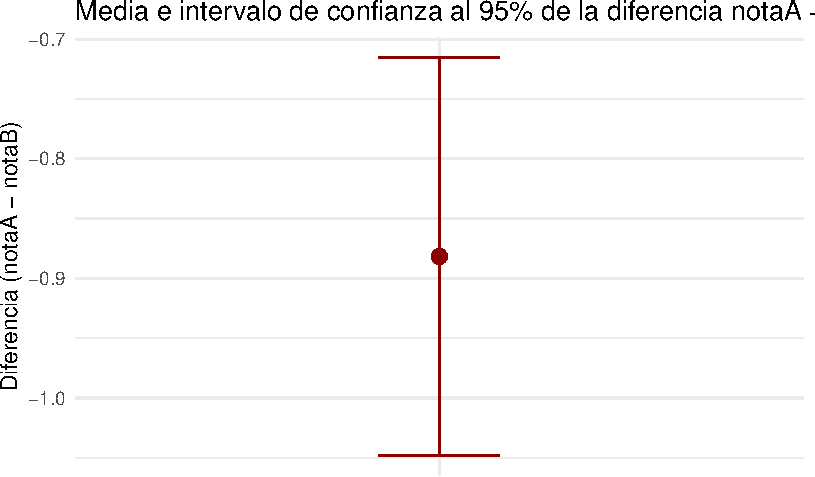
\includegraphics[keepaspectratio]{13-contrastes-dos-poblaciones-pareadas_files/figure-pdf/unnamed-chunk-8-1.pdf}}

El test t para datos pareados proporciona un estadístico \(t=-10.51\)
con 114 grados de libertad y un p-valor menor que \(2.2\times10^{-16}\),
muy inferior a 0.05, por lo que se rechaza la hipótesis nula
\(H_0: \mu_D=0\). La media estimada de la diferencia es -0.88, con un
intervalo de confianza al 95\% de \((-1.05, -0.72)\), que no contiene el
0. Se concluye, por tanto, que existe una diferencia significativa entre
las notas medias de las asignaturas A y B para los mismos alumnos,
siendo la nota media de la asignatura B significativamente superior a la
de la asignatura A.

\end{example}

\subsection{Test de Wilcoxon para datos
pareados}\label{test-de-wilcoxon-para-datos-pareados}

\begin{definition}[Test de Wilcoxon para datos
pareados]\protect\hypertarget{def-dospareadas-wilcoxon-pareado}{}\label{def-dospareadas-wilcoxon-pareado}

El \emph{test de Wilcoxon para datos pareados} (o test de los rangos con
signo de Wilcoxon) es la alternativa no paramétrica al test t para datos
pareados. Contrasta si existe diferencia entre las distribuciones
(habitualmente interpretada como diferencia entre las medianas) de dos
poblaciones pareadas, sin necesidad de asumir normalidad de la
diferencia. La hipótesis nula es

\[H_0: \text{la distribución de las diferencias es simétrica en torno a 0}\]

frente a la alternativa de que existe un desplazamiento sistemático de
las diferencias por encima o por debajo de 0.

\end{definition}

\textbf{Requisitos}:

\begin{itemize}
\tightlist
\item
  La variable dependiente es cuantitativa (o al menos ordinal) y se mide
  dos veces sobre los mismos individuos.
\item
  No se requiere que la diferencia siga una distribución normal, lo que
  lo hace preferible al test t para datos pareados cuando ese supuesto
  no se cumple o el tamaño muestral es pequeño.
\end{itemize}

Aunque en el ejemplo anterior la diferencia \texttt{diferencia\_AB} pudo
asumirse normal y el test t era plenamente aplicable, se ilustra a
continuación su alternativa no paramétrica, útil como contraste de
robustez o para las situaciones en las que la normalidad de la
diferencia no pueda asumirse.

\begin{example}[]\protect\hypertarget{exm-dospareadas-wilcoxon-pareado}{}\label{exm-dospareadas-wilcoxon-pareado}

~

\begin{Shaded}
\begin{Highlighting}[]
\FunctionTok{wilcox.test}\NormalTok{(df}\SpecialCharTok{$}\NormalTok{notaA, df}\SpecialCharTok{$}\NormalTok{notaB, }\AttributeTok{alternative =} \StringTok{"two.sided"}\NormalTok{, }\AttributeTok{paired =} \ConstantTok{TRUE}\NormalTok{)}
\end{Highlighting}
\end{Shaded}

\begin{verbatim}

    Wilcoxon signed rank test with continuity correction

data:  df$notaA and df$notaB
V = 398, p-value = 2.442e-15
alternative hypothesis: true location shift is not equal to 0
\end{verbatim}

El test de Wilcoxon para datos pareados proporciona un estadístico
\(V=398\) y un p-valor de \(2.44\times10^{-15}\), muy inferior a 0.05,
por lo que se rechaza la hipótesis nula de simetría de las diferencias
en torno a 0. La conclusión coincide con la del test t: existe una
diferencia significativa entre las calificaciones de los mismos alumnos
en las asignaturas A y B.

\end{example}

\section{\texorpdfstring{Variable dependiente cualitativa: comparar
\texttt{calificacionA} con
\texttt{calificacionB}}{Variable dependiente cualitativa: comparar calificacionA con calificacionB}}\label{variable-dependiente-cualitativa-comparar-calificaciona-con-calificacionb}

Las variables \texttt{calificacionA} y \texttt{calificacionB} recogen,
para los mismos 120 alumnos, el resultado cualitativo (Aprobado /
Suspenso) de las asignaturas A y B. Al tratarse de la misma pareja de
alumnos medidos dos veces con una variable cualitativa binaria, no puede
aplicarse aquí un contraste de independencia habitual, sino uno diseñado
específicamente para datos pareados.

\subsection{Test de McNemar}\label{test-de-mcnemar}

\begin{definition}[Test de
McNemar]\protect\hypertarget{def-dospareadas-mcnemar}{}\label{def-dospareadas-mcnemar}

El \emph{test de McNemar} contrasta si la proporción de una categoría de
una variable cualitativa binaria cambia entre dos mediciones pareadas
realizadas sobre los mismos individuos. Si \(b\) es el número de
individuos que pasan de la categoría 1 a la categoría 2 entre la primera
y la segunda medición, y \(c\) el número de individuos que pasan de la
categoría 2 a la categoría 1, la hipótesis nula es

\[H_0: p_b = p_c\]

es decir, que las proporciones marginales de las dos mediciones son
iguales, o equivalentemente, que no hay un cambio neto entre la primera
y la segunda medición (los cambios en un sentido y en el otro se
compensan).

\end{definition}

\textbf{Requisitos}:

\begin{itemize}
\tightlist
\item
  La variable dependiente es cualitativa binaria (dos categorías) y se
  mide dos veces sobre los mismos individuos.
\item
  Los datos se organizan en una tabla de contingencia 2x2
  \textbf{pareada}, en la que filas y columnas representan las
  categorías de la misma variable en la primera y en la segunda
  medición, y cada individuo contribuye a una única celda.
\end{itemize}

Nótese que en esta situación no puede utilizarse el test chi-cuadrado de
independencia empleado en el capítulo de
\hyperref[contrastes-para-dos-poblaciones-independientes]{contrastes
para dos poblaciones independientes}: allí las dos poblaciones
comparadas estaban formadas por individuos distintos, de modo que cada
observación era independiente de las demás, condición que exige el test
chi-cuadrado. Aquí, en cambio, cada uno de los 120 alumnos aparece dos
veces en la tabla (una en \texttt{calificacionA} y otra en
\texttt{calificacionB}), por lo que las observaciones no son
independientes entre sí, y aplicar un chi-cuadrado de independencia
estándar sería incorrecto. El test de McNemar resuelve este problema
centrándose únicamente en los alumnos que cambian de categoría entre las
dos mediciones.

\begin{example}[]\protect\hypertarget{exm-dospareadas-mcnemar}{}\label{exm-dospareadas-mcnemar}

~

\begin{Shaded}
\begin{Highlighting}[]
\NormalTok{tabla }\OtherTok{\textless{}{-}} \FunctionTok{table}\NormalTok{(df}\SpecialCharTok{$}\NormalTok{calificacionA, df}\SpecialCharTok{$}\NormalTok{calificacionB)}
\NormalTok{tabla}
\end{Highlighting}
\end{Shaded}

\begin{verbatim}
          
           Aprobado Suspenso
  Aprobado       86        3
  Suspenso       12       14
\end{verbatim}

\begin{Shaded}
\begin{Highlighting}[]
\FunctionTok{mcnemar.test}\NormalTok{(tabla, }\AttributeTok{correct =} \ConstantTok{TRUE}\NormalTok{)}
\end{Highlighting}
\end{Shaded}

\begin{verbatim}

    McNemar's Chi-squared test with continuity correction

data:  tabla
McNemar's chi-squared = 4.2667, df = 1, p-value = 0.03887
\end{verbatim}

De los 115 alumnos con calificación registrada en ambas asignaturas, 86
aprueban las dos y 14 suspenden las dos: estos alumnos no cambian de
categoría y no aportan información al contraste. De los 29 alumnos
restantes, 12 suspenden la asignatura A pero aprueban la B, mientras que
solo 3 aprueban la A y suspenden la B. El test de McNemar, aplicado
sobre estos cambios discordantes, proporciona un estadístico
\(\chi^2=4.27\) con 1 grado de libertad y un p-valor de 0.039, menor que
0.05, por lo que se rechaza la hipótesis nula de igualdad de
proporciones marginales. Se concluye que la proporción de aprobados no
es la misma en la asignatura A que en la B para los mismos alumnos: de
hecho, la proporción de aprobados pasa del 77.4\% (89 de 115) en la
asignatura A al 85.2\% (98 de 115) en la asignatura B, un aumento que
resulta ser estadísticamente significativo.

\end{example}

\section{Para saber más}\label{para-saber-muxe1s}

Este capítulo ha cubierto el caso de dos mediciones pareadas. Cuando las
dos poblaciones comparadas están formadas por individuos distintos, sin
ninguna relación entre ellos, el contraste adecuado es el que se
presenta en el capítulo de
\hyperref[contrastes-para-dos-poblaciones-independientes]{contrastes
para dos poblaciones independientes}. Y cuando se dispone de más de dos
medidas repetidas sobre los mismos individuos (por ejemplo, las cinco
notas \texttt{notaA} a \texttt{notaE} de cada alumno, en lugar de solo
dos), los contrastes t y de Wilcoxon para datos pareados dejan de ser
aplicables y hay que recurrir a los que se presentan en el capítulo de
\href{15-contrastes-medidas-repetidas.qmd}{contrastes para más de dos
poblaciones relacionadas}.

\chapter{Contrastes para más de dos poblaciones
independientes}\label{contrastes-para-muxe1s-de-dos-poblaciones-independientes}

El \hyperref[contrastes-para-dos-poblaciones-independientes]{capítulo
anterior} trató el caso de dos poblaciones independientes. Sin embargo,
en muchas ocasiones no se comparan dos grupos, sino tres o más, formados
por individuos distintos entre sí. Este capítulo generaliza los
contrastes anteriores a esa situación: cómo comparar una variable,
cuantitativa o cualitativa, entre más de dos poblaciones independientes.
En el conjunto de datos de ejemplo, la variable independiente natural
para esta situación es \texttt{grupo}, que clasifica a los 120 alumnos
en tres grupos de clase (A, B y C), formados por alumnos distintos:
nadie pertenece a la vez a dos grupos, por lo que las tres poblaciones
son independientes entre sí.

\section{Estadísticos descriptivos por
grupo}\label{estaduxedsticos-descriptivos-por-grupo-1}

Antes de aplicar ningún contraste, conviene describir la variable
cuantitativa de interés en cada uno de los grupos. Se utiliza aquí la
variable \texttt{notaC}, que es la que muestra diferencias más claras
entre los tres grupos de clase.

\begin{Shaded}
\begin{Highlighting}[]
\FunctionTok{library}\NormalTok{(moments)}

\NormalTok{df }\SpecialCharTok{|\textgreater{}}
  \FunctionTok{group\_by}\NormalTok{(grupo) }\SpecialCharTok{|\textgreater{}}
  \FunctionTok{summarise}\NormalTok{(}
    \AttributeTok{n =} \FunctionTok{sum}\NormalTok{(}\SpecialCharTok{!}\FunctionTok{is.na}\NormalTok{(notaC)),}
    \AttributeTok{media =} \FunctionTok{mean}\NormalTok{(notaC, }\AttributeTok{na.rm =} \ConstantTok{TRUE}\NormalTok{),}
    \AttributeTok{de =} \FunctionTok{sd}\NormalTok{(notaC, }\AttributeTok{na.rm =} \ConstantTok{TRUE}\NormalTok{),}
    \AttributeTok{minimo =} \FunctionTok{min}\NormalTok{(notaC, }\AttributeTok{na.rm =} \ConstantTok{TRUE}\NormalTok{),}
    \AttributeTok{q1 =} \FunctionTok{quantile}\NormalTok{(notaC, }\FloatTok{0.25}\NormalTok{, }\AttributeTok{na.rm =} \ConstantTok{TRUE}\NormalTok{),}
    \AttributeTok{mediana =} \FunctionTok{median}\NormalTok{(notaC, }\AttributeTok{na.rm =} \ConstantTok{TRUE}\NormalTok{),}
    \AttributeTok{q3 =} \FunctionTok{quantile}\NormalTok{(notaC, }\FloatTok{0.75}\NormalTok{, }\AttributeTok{na.rm =} \ConstantTok{TRUE}\NormalTok{),}
    \AttributeTok{maximo =} \FunctionTok{max}\NormalTok{(notaC, }\AttributeTok{na.rm =} \ConstantTok{TRUE}\NormalTok{),}
    \AttributeTok{asimetria =} \FunctionTok{skewness}\NormalTok{(notaC, }\AttributeTok{na.rm =} \ConstantTok{TRUE}\NormalTok{),}
    \AttributeTok{apuntamiento =} \FunctionTok{kurtosis}\NormalTok{(notaC, }\AttributeTok{na.rm =} \ConstantTok{TRUE}\NormalTok{)}
\NormalTok{  )}
\end{Highlighting}
\end{Shaded}

\begin{verbatim}
# A tibble: 3 x 11
  grupo     n media    de minimo    q1 mediana    q3 maximo asimetria
  <chr> <int> <dbl> <dbl>  <dbl> <dbl>   <dbl> <dbl>  <dbl>     <dbl>
1 A        38  5.52  1.51    2     4.6    5.55   6.5    9.5    0.0121
2 B        34  5.95  1.35    2.8   5.3    6      6.9    8.8   -0.473 
3 C        47  4.07  1.38    1.3   3.3    4      5.1    6.7   -0.0272
# i 1 more variable: apuntamiento <dbl>
\end{verbatim}

El grupo C presenta la media más baja (4.07) y los grupos A y B medias
parecidas y más altas (5.52 y 5.95, respectivamente), lo que ya sugiere
que podría existir una diferencia real entre C y los otros dos grupos.
Las tres distribuciones tienen una asimetría cercana a 0 y un
apuntamiento próximo a 3, lo que es compatible con una distribución
aproximadamente normal en los tres grupos.

\textbf{Gráficos.} Un diagrama de cajas y bigotes y un diagrama de
violín permiten visualizar de un vistazo estas diferencias:

\begin{Shaded}
\begin{Highlighting}[]
\FunctionTok{ggplot}\NormalTok{(df, }\FunctionTok{aes}\NormalTok{(}\AttributeTok{x =}\NormalTok{ grupo, }\AttributeTok{y =}\NormalTok{ notaC, }\AttributeTok{fill =}\NormalTok{ grupo)) }\SpecialCharTok{+}
  \FunctionTok{geom\_boxplot}\NormalTok{() }\SpecialCharTok{+}
  \FunctionTok{labs}\NormalTok{(}\AttributeTok{x =} \StringTok{"Grupo"}\NormalTok{, }\AttributeTok{y =} \StringTok{"Nota C"}\NormalTok{) }\SpecialCharTok{+}
  \FunctionTok{theme\_minimal}\NormalTok{() }\SpecialCharTok{+}
  \FunctionTok{theme}\NormalTok{(}\AttributeTok{legend.position =} \StringTok{"none"}\NormalTok{)}
\end{Highlighting}
\end{Shaded}

\begin{figure}[H]

{\centering \pandocbounded{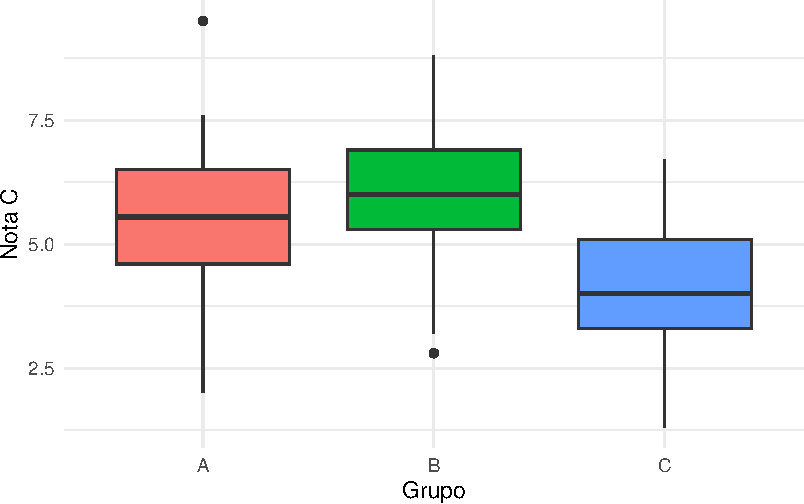
\includegraphics[keepaspectratio]{14-contrastes-mas-dos-poblaciones-independientes_files/figure-pdf/boxplot-1.pdf}}

}

\caption{Diagrama de cajas y bigotes de la nota C por grupo.}

\end{figure}%

\begin{Shaded}
\begin{Highlighting}[]
\FunctionTok{ggplot}\NormalTok{(df, }\FunctionTok{aes}\NormalTok{(}\AttributeTok{x =}\NormalTok{ grupo, }\AttributeTok{y =}\NormalTok{ notaC, }\AttributeTok{fill =}\NormalTok{ grupo)) }\SpecialCharTok{+}
  \FunctionTok{geom\_violin}\NormalTok{() }\SpecialCharTok{+}
  \FunctionTok{labs}\NormalTok{(}\AttributeTok{x =} \StringTok{"Grupo"}\NormalTok{, }\AttributeTok{y =} \StringTok{"Nota C"}\NormalTok{) }\SpecialCharTok{+}
  \FunctionTok{theme\_minimal}\NormalTok{() }\SpecialCharTok{+}
  \FunctionTok{theme}\NormalTok{(}\AttributeTok{legend.position =} \StringTok{"none"}\NormalTok{)}
\end{Highlighting}
\end{Shaded}

\begin{figure}[H]

{\centering \pandocbounded{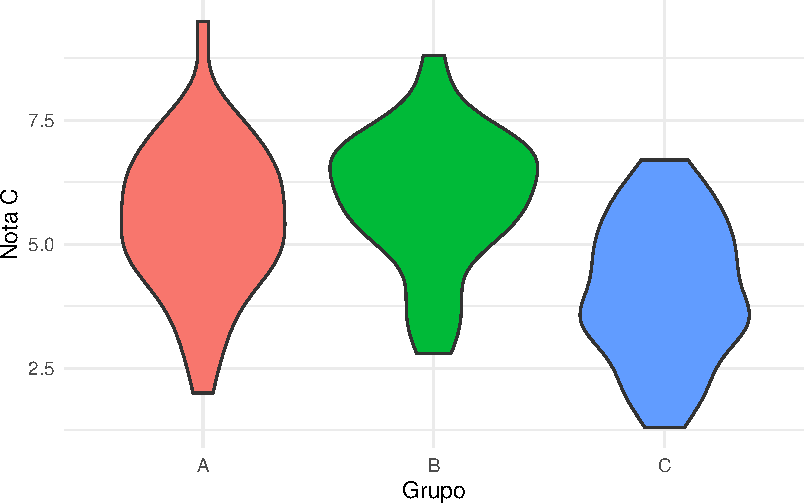
\includegraphics[keepaspectratio]{14-contrastes-mas-dos-poblaciones-independientes_files/figure-pdf/violin-1.pdf}}

}

\caption{Diagrama de violín de la nota C por grupo.}

\end{figure}%

En ambos gráficos se aprecia que el grupo C tiene una posición más baja
que A y B, y que las cajas de A y B se solapan bastante, mientras que la
de C apenas se solapa con ellas.

\textbf{Normalidad por grupo.} Antes de decidir qué contraste aplicar
(paramétrico o no paramétrico), es necesario comprobar si \texttt{notaC}
sigue una distribución normal en cada uno de los tres grupos, mediante
el test de Shapiro-Wilk:

\begin{Shaded}
\begin{Highlighting}[]
\NormalTok{df }\SpecialCharTok{|\textgreater{}}
  \FunctionTok{filter}\NormalTok{(}\SpecialCharTok{!}\FunctionTok{is.na}\NormalTok{(notaC)) }\SpecialCharTok{|\textgreater{}}
  \FunctionTok{group\_by}\NormalTok{(grupo) }\SpecialCharTok{|\textgreater{}}
  \FunctionTok{summarise}\NormalTok{(}
    \AttributeTok{estadistico =} \FunctionTok{shapiro.test}\NormalTok{(notaC)}\SpecialCharTok{$}\NormalTok{statistic,}
    \AttributeTok{p.valor =} \FunctionTok{shapiro.test}\NormalTok{(notaC)}\SpecialCharTok{$}\NormalTok{p.value}
\NormalTok{  )}
\end{Highlighting}
\end{Shaded}

\begin{verbatim}
# A tibble: 3 x 3
  grupo estadistico p.valor
  <chr>       <dbl>   <dbl>
1 A           0.989   0.961
2 B           0.965   0.343
3 C           0.976   0.442
\end{verbatim}

En los tres grupos el p-valor es muy superior a 0.05 (0.9614 en A,
0.3432 en B y 0.4420 en C), por lo que no hay evidencia para rechazar la
normalidad de \texttt{notaC} en ninguno de ellos. Se cumple, por tanto,
el requisito de normalidad necesario para aplicar los contrastes
paramétricos que siguen.

\subsection{Test de Levene de comparación de
varianzas}\label{test-de-levene-de-comparaciuxf3n-de-varianzas}

\begin{definition}[Test de Levene de comparación de
varianzas]\protect\hypertarget{def-masdosindep-levene}{}\label{def-masdosindep-levene}

El \emph{test de Levene} tiene como objetivo contrastar si las varianzas
de una variable cuantitativa son iguales en más de dos poblaciones
independientes. Es la generalización a más de dos grupos del test F de
Fisher visto en el capítulo anterior. Las hipótesis del contraste son

\[H_0: \sigma_1^2=\sigma_2^2=\cdots=\sigma_k^2 \quad \text{frente a} \quad H_1: \text{algún } \sigma_i^2 \text{ es distinto de los demás},\]

donde \(k\) es el número de poblaciones comparadas.

\end{definition}

\begin{tcolorbox}[enhanced jigsaw, arc=.35mm, bottomrule=.15mm, bottomtitle=1mm, breakable, colback=white, colbacktitle=quarto-callout-note-color!10!white, colframe=quarto-callout-note-color-frame, coltitle=black, left=2mm, leftrule=.75mm, opacityback=0, opacitybacktitle=0.6, rightrule=.15mm, title=\textcolor{quarto-callout-note-color}{\faInfo}\hspace{0.5em}{Interpretación}, titlerule=0mm, toprule=.15mm, toptitle=1mm]

\begin{itemize}
\tightlist
\item
  Si el p-valor del contraste es mayor que el nivel de significación
  (habitualmente 0.05), no se rechaza \(H_0\) y se concluye que las
  varianzas de los \(k\) grupos pueden considerarse homogéneas.
\item
  Si el p-valor es menor que el nivel de significación, se rechaza
  \(H_0\) y se concluye que al menos uno de los grupos tiene una
  varianza distinta de las demás.
\item
  Comprobar la homogeneidad de varianzas es un paso previo necesario
  para poder aplicar después el ANOVA de un factor, ya que este último
  asume que las varianzas de los grupos son iguales.
\end{itemize}

\end{tcolorbox}

\textbf{Requisitos}:

\begin{itemize}
\tightlist
\item
  La variable comparada debe ser cuantitativa.
\item
  Las poblaciones comparadas deben ser independientes entre sí
  (individuos distintos en cada grupo).
\item
  La variable debe seguir una distribución normal en todos los grupos, o
  bien el tamaño de cada grupo debe ser igual o superior a 30 (en cuyo
  caso el teorema central del límite garantiza una aproximación
  razonable).
\end{itemize}

Comprobada la normalidad de \texttt{notaC} en los tres grupos, se puede
aplicar el test de Levene con la función \texttt{leveneTest()} del
paquete \texttt{car} para contrastar si las tres poblaciones tienen la
misma varianza.

\begin{example}[]\protect\hypertarget{exm-masdosindep-levene}{}\label{exm-masdosindep-levene}

~

\begin{Shaded}
\begin{Highlighting}[]
\FunctionTok{library}\NormalTok{(car)}

\NormalTok{df }\OtherTok{\textless{}{-}}\NormalTok{ df }\SpecialCharTok{|\textgreater{}} \FunctionTok{mutate}\NormalTok{(}\AttributeTok{grupo =} \FunctionTok{factor}\NormalTok{(grupo))}
\FunctionTok{leveneTest}\NormalTok{(notaC }\SpecialCharTok{\textasciitilde{}}\NormalTok{ grupo, }\AttributeTok{data =}\NormalTok{ df)}
\end{Highlighting}
\end{Shaded}

\begin{verbatim}
Levene's Test for Homogeneity of Variance (center = median)
       Df F value Pr(>F)
group   2  0.3186 0.7278
      116               
\end{verbatim}

El p-valor del contraste es 0.7278, muy superior a 0.05, por lo que no
se rechaza \(H_0\): no hay evidencia de que las varianzas de
\texttt{notaC} difieran entre los tres grupos de clase. Se cumple, por
tanto, el requisito de homogeneidad de varianzas necesario para aplicar
el ANOVA de un factor.

\end{example}

\subsection{ANOVA de un factor}\label{anova-de-un-factor}

\begin{definition}[ANOVA de un
factor]\protect\hypertarget{def-masdosindep-anova}{}\label{def-masdosindep-anova}

El \emph{análisis de varianza (ANOVA) de un factor} tiene como objetivo
contrastar si existen diferencias entre las medias de una variable
cuantitativa en más de dos poblaciones independientes. Las hipótesis del
contraste son

\[H_0: \mu_1=\mu_2=\cdots=\mu_k \quad \text{frente a} \quad H_1: \text{alguna } \mu_i \text{ es distinta de las demás},\]

donde \(k\) es el número de poblaciones comparadas.

\end{definition}

\begin{tcolorbox}[enhanced jigsaw, arc=.35mm, bottomrule=.15mm, bottomtitle=1mm, breakable, colback=white, colbacktitle=quarto-callout-note-color!10!white, colframe=quarto-callout-note-color-frame, coltitle=black, left=2mm, leftrule=.75mm, opacityback=0, opacitybacktitle=0.6, rightrule=.15mm, title=\textcolor{quarto-callout-note-color}{\faInfo}\hspace{0.5em}{Interpretación}, titlerule=0mm, toprule=.15mm, toptitle=1mm]

\begin{itemize}
\tightlist
\item
  Si el p-valor del contraste es mayor que 0.05, no se rechaza \(H_0\) y
  se concluye que no hay evidencia de diferencias entre las medias de
  los \(k\) grupos.
\item
  Si el p-valor es menor que 0.05, se rechaza \(H_0\) y se concluye que
  al menos una de las medias difiere de las demás, aunque el ANOVA por
  sí solo no indica cuál o cuáles.
\item
  El ANOVA de un factor es la generalización a más de dos grupos del
  test t de comparación de medias visto en el capítulo anterior: de
  hecho, cuando \(k=2\), ambos contrastes son equivalentes.
\end{itemize}

\end{tcolorbox}

\textbf{Requisitos}:

\begin{itemize}
\tightlist
\item
  La variable dependiente debe ser cuantitativa.
\item
  Las poblaciones comparadas deben ser independientes entre sí.
\item
  La variable debe seguir una distribución normal en cada uno de los
  grupos, o los grupos deben tener un tamaño igual o superior a 30.
\item
  Las varianzas de los grupos deben ser homogéneas, requisito que se
  comprueba previamente con el test de Levene.
\end{itemize}

Como se cumplen los requisitos de normalidad y homogeneidad de
varianzas, se puede aplicar el ANOVA de un factor con la función
\texttt{aov()} para contrastar si existen diferencias entre las medias
de \texttt{notaC} en los tres grupos.

\begin{example}[]\protect\hypertarget{exm-masdosindep-anova}{}\label{exm-masdosindep-anova}

~

\begin{Shaded}
\begin{Highlighting}[]
\NormalTok{modelo\_anova }\OtherTok{\textless{}{-}} \FunctionTok{aov}\NormalTok{(notaC }\SpecialCharTok{\textasciitilde{}}\NormalTok{ grupo, }\AttributeTok{data =}\NormalTok{ df)}
\FunctionTok{summary}\NormalTok{(modelo\_anova)}
\end{Highlighting}
\end{Shaded}

\begin{verbatim}
             Df Sum Sq Mean Sq F value   Pr(>F)    
grupo         2  80.69   40.34   20.05 3.32e-08 ***
Residuals   116 233.41    2.01                     
---
Signif. codes:  0 '***' 0.001 '**' 0.01 '*' 0.05 '.' 0.1 ' ' 1
1 observation deleted due to missingness
\end{verbatim}

El p-valor del contraste (\texttt{Pr(\textgreater{}F)}) es 3.32e-08, muy
inferior a 0.05, por lo que se rechaza \(H_0\): existen diferencias
significativas entre las medias de \texttt{notaC} en al menos dos de los
tres grupos de clase.

\end{example}

Cuando, como en este caso, el ANOVA resulta significativo, este solo
informa de que existe alguna diferencia entre los grupos, pero no indica
entre cuáles. Es necesario entonces aplicar un \textbf{test de
comparación múltiple por pares} que compare las medias de los grupos dos
a dos, controlando el error global de realizar varias comparaciones
simultáneas. El más habitual es el \textbf{test de Tukey}
(\texttt{TukeyHSD()}), aunque también se utiliza, de forma algo más
conservadora, la corrección de \textbf{Bonferroni}, que simplemente
divide el nivel de significación entre el número de comparaciones
realizadas.

\begin{Shaded}
\begin{Highlighting}[]
\FunctionTok{TukeyHSD}\NormalTok{(modelo\_anova)}
\end{Highlighting}
\end{Shaded}

\begin{verbatim}
  Tukey multiple comparisons of means
    95% family-wise confidence level

Fit: aov(formula = notaC ~ grupo, data = df)

$grupo
          diff        lwr        upr     p adj
B-A  0.4312693 -0.3637573  1.2262960 0.4048482
C-A -1.4455767 -2.1802858 -0.7108676 0.0000241
C-B -1.8768461 -2.6350758 -1.1186163 0.0000001
\end{verbatim}

Los resultados muestran que la diferencia entre B y A no es
significativa (p-valor 0.4048), mientras que las diferencias entre C y A
(p-valor 0.0000241) y entre C y B (p-valor 0.0000001) sí lo son. Es
decir, el grupo C tiene una nota media en \texttt{notaC}
significativamente inferior a la de los otros dos grupos, mientras que A
y B no difieren significativamente entre sí.

Un diagrama de medias con sus intervalos de confianza al 95\% permite
visualizar estas mismas conclusiones:

\begin{Shaded}
\begin{Highlighting}[]
\NormalTok{mean\_ci }\OtherTok{\textless{}{-}} \ControlFlowTok{function}\NormalTok{(x) \{}
\NormalTok{  x }\OtherTok{\textless{}{-}}\NormalTok{ x[}\SpecialCharTok{!}\FunctionTok{is.na}\NormalTok{(x)]}
\NormalTok{  m }\OtherTok{\textless{}{-}} \FunctionTok{mean}\NormalTok{(x)}
\NormalTok{  se }\OtherTok{\textless{}{-}} \FunctionTok{sd}\NormalTok{(x) }\SpecialCharTok{/} \FunctionTok{sqrt}\NormalTok{(}\FunctionTok{length}\NormalTok{(x))}
\NormalTok{  ic }\OtherTok{\textless{}{-}}\NormalTok{ se }\SpecialCharTok{*} \FunctionTok{qt}\NormalTok{(}\FloatTok{0.975}\NormalTok{, }\FunctionTok{length}\NormalTok{(x) }\SpecialCharTok{{-}} \DecValTok{1}\NormalTok{)}
  \FunctionTok{data.frame}\NormalTok{(}\AttributeTok{y =}\NormalTok{ m, }\AttributeTok{ymin =}\NormalTok{ m }\SpecialCharTok{{-}}\NormalTok{ ic, }\AttributeTok{ymax =}\NormalTok{ m }\SpecialCharTok{+}\NormalTok{ ic)}
\NormalTok{\}}

\FunctionTok{ggplot}\NormalTok{(df, }\FunctionTok{aes}\NormalTok{(}\AttributeTok{x =}\NormalTok{ grupo, }\AttributeTok{y =}\NormalTok{ notaC, }\AttributeTok{color =}\NormalTok{ grupo)) }\SpecialCharTok{+}
  \FunctionTok{stat\_summary}\NormalTok{(}\AttributeTok{fun.data =}\NormalTok{ mean\_ci, }\AttributeTok{geom =} \StringTok{"errorbar"}\NormalTok{, }\AttributeTok{width =} \FloatTok{0.2}\NormalTok{) }\SpecialCharTok{+}
  \FunctionTok{stat\_summary}\NormalTok{(}\AttributeTok{fun =}\NormalTok{ mean, }\AttributeTok{geom =} \StringTok{"point"}\NormalTok{, }\AttributeTok{size =} \DecValTok{3}\NormalTok{) }\SpecialCharTok{+}
  \FunctionTok{labs}\NormalTok{(}\AttributeTok{x =} \StringTok{"Grupo"}\NormalTok{, }\AttributeTok{y =} \StringTok{"Nota C media"}\NormalTok{) }\SpecialCharTok{+}
  \FunctionTok{theme\_minimal}\NormalTok{() }\SpecialCharTok{+}
  \FunctionTok{theme}\NormalTok{(}\AttributeTok{legend.position =} \StringTok{"none"}\NormalTok{)}
\end{Highlighting}
\end{Shaded}

\begin{figure}[H]

{\centering \pandocbounded{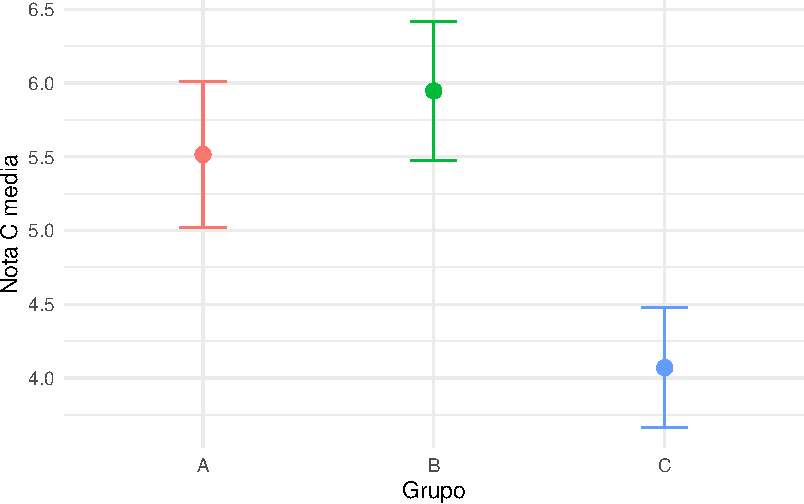
\includegraphics[keepaspectratio]{14-contrastes-mas-dos-poblaciones-independientes_files/figure-pdf/medias-ic-1.pdf}}

}

\caption{Medias de la nota C por grupo con intervalos de confianza al
95\%.}

\end{figure}%

En el gráfico se aprecia que los intervalos de confianza de A y B se
solapan ampliamente, mientras que el de C queda claramente por debajo y
no se solapa con los de los otros dos grupos, en consonancia con el
resultado del test de Tukey.

\subsection{Test de Kruskal-Wallis (no
paramétrico)}\label{test-de-kruskal-wallis-no-paramuxe9trico}

\begin{definition}[Test de
Kruskal-Wallis]\protect\hypertarget{def-masdosindep-kruskal}{}\label{def-masdosindep-kruskal}

El \emph{test de Kruskal-Wallis} es la alternativa no paramétrica al
ANOVA de un factor. Tiene como objetivo contrastar si las distribuciones
de una variable cuantitativa u ordinal son iguales en más de dos
poblaciones independientes, sin necesidad de asumir normalidad. Las
hipótesis del contraste son

\[H_0: \text{las distribuciones (medianas) son iguales en las } k \text{ poblaciones} \quad \text{frente a} \quad H_1: \text{alguna difiere de las demás}.\]

\end{definition}

\begin{tcolorbox}[enhanced jigsaw, arc=.35mm, bottomrule=.15mm, bottomtitle=1mm, breakable, colback=white, colbacktitle=quarto-callout-note-color!10!white, colframe=quarto-callout-note-color-frame, coltitle=black, left=2mm, leftrule=.75mm, opacityback=0, opacitybacktitle=0.6, rightrule=.15mm, title=\textcolor{quarto-callout-note-color}{\faInfo}\hspace{0.5em}{Interpretación}, titlerule=0mm, toprule=.15mm, toptitle=1mm]

\begin{itemize}
\tightlist
\item
  Si el p-valor del contraste es mayor que 0.05, no se rechaza \(H_0\) y
  se concluye que no hay evidencia de diferencias entre las
  distribuciones de los \(k\) grupos.
\item
  Si el p-valor es menor que 0.05, se rechaza \(H_0\) y se concluye que
  al menos una de las distribuciones difiere de las demás.
\item
  El test de Kruskal-Wallis es la generalización a más de dos grupos del
  test U de Mann-Whitney visto en el capítulo anterior, del mismo modo
  que el ANOVA generaliza al test t.
\end{itemize}

\end{tcolorbox}

\textbf{Requisitos}:

\begin{itemize}
\tightlist
\item
  La variable comparada debe ser, al menos, ordinal (cuantitativa o
  cualitativa ordinal).
\item
  Las poblaciones comparadas deben ser independientes entre sí.
\item
  A diferencia del ANOVA, no exige que la variable siga una distribución
  normal en los grupos, lo que lo convierte en la alternativa natural
  cuando no se cumple ese requisito o cuando la variable es solo
  ordinal.
\end{itemize}

Cuando no se cumple el requisito de normalidad del ANOVA (o directamente
se quiere evitar esa suposición), se recurre al test de Kruskal-Wallis.
A modo de ejemplo, se aplica ahora a la variable \texttt{notaA}, que no
se ha comprobado que sea normal en los tres grupos:

\begin{example}[]\protect\hypertarget{exm-masdosindep-kruskal}{}\label{exm-masdosindep-kruskal}

~

\begin{Shaded}
\begin{Highlighting}[]
\FunctionTok{kruskal.test}\NormalTok{(notaA }\SpecialCharTok{\textasciitilde{}}\NormalTok{ grupo, }\AttributeTok{data =}\NormalTok{ df)}
\end{Highlighting}
\end{Shaded}

\begin{verbatim}

    Kruskal-Wallis rank sum test

data:  notaA by grupo
Kruskal-Wallis chi-squared = 62.218, df = 2, p-value = 3.087e-14
\end{verbatim}

El p-valor del contraste es 3.087e-14, muy inferior a 0.05, por lo que
se rechaza \(H_0\): existen diferencias significativas entre las
distribuciones de \texttt{notaA} en al menos dos de los tres grupos.

\end{example}

Igual que ocurre con el ANOVA, un resultado significativo en el test de
Kruskal-Wallis no indica entre qué grupos concretos hay diferencias. El
test de comparación múltiple por pares equivalente es el \textbf{test de
Wilcoxon por pares}, aplicando una corrección (aquí, el método de
Benjamini-Hochberg, \texttt{"BH"}) para controlar el error acumulado al
hacer varias comparaciones:

\begin{Shaded}
\begin{Highlighting}[]
\FunctionTok{pairwise.wilcox.test}\NormalTok{(df}\SpecialCharTok{$}\NormalTok{notaA, df}\SpecialCharTok{$}\NormalTok{grupo, }\AttributeTok{p.adjust.method =} \StringTok{"BH"}\NormalTok{)}
\end{Highlighting}
\end{Shaded}

\begin{verbatim}

    Pairwise comparisons using Wilcoxon rank sum test with continuity correction 

data:  df$notaA and df$grupo 

  A       B      
B 0.19    -      
C 4.2e-10 1.3e-11

P value adjustment method: BH 
\end{verbatim}

La diferencia entre A y B no es significativa (p-valor 0.19), mientras
que las diferencias entre A y C (p-valor 4.2e-10) y entre B y C (p-valor
1.3e-11) sí lo son. La conclusión es, por tanto, coherente con la
obtenida antes para \texttt{notaC}: el grupo C se diferencia claramente
de los otros dos, que no difieren significativamente entre sí.

\section{Variable dependiente
cualitativa}\label{variable-dependiente-cualitativa-1}

Cuando la variable dependiente es cualitativa y se compara entre más de
dos poblaciones independientes, el contraste apropiado sigue siendo el
\textbf{test Chi-cuadrado de independencia}, ya presentado en el
capítulo de
\hyperref[contrastes-para-dos-poblaciones-independientes]{Contrastes
para dos poblaciones independientes}. Allí se aplicaba a una tabla de
contingencia \(2\times2\), construida cruzando una variable
independiente con dos categorías y una variable dependiente también con
dos categorías; aquí la única diferencia es que la tabla de contingencia
tiene más de dos filas (o más de dos columnas), al tener \texttt{grupo}
tres categorías en lugar de dos.

Así, para contrastar si existe relación entre el grupo de clase y el
resultado (aprobado o suspenso) en la asignatura A, bastaría con
construir la tabla de contingencia
\texttt{table(df\$grupo,\ df\$calificacionA)}, de dimensión
\(3\times2\), y aplicar sobre ella \texttt{chisq.test()} exactamente
igual que en el caso de dos grupos. El estadístico de contraste, sus
grados de libertad (que ahora dependen del número de filas y columnas de
la tabla) y la interpretación del p-valor obtenido no cambian en
absoluto respecto al procedimiento ya descrito para dos poblaciones
independientes.

\section{Cierre}\label{cierre}

Este capítulo ha mostrado cómo comparar más de dos poblaciones
independientes, tanto cuando la variable dependiente es cuantitativa
(Levene, ANOVA y Tukey, o su alternativa no paramétrica, Kruskal-Wallis
con comparaciones de Wilcoxon por pares) como cuando es cualitativa
(Chi-cuadrado de independencia). El siguiente capítulo,
\href{15-contrastes-medidas-repetidas.qmd}{Contrastes para más de dos
poblaciones relacionadas}, trata la situación análoga pero cuando los
más de dos grupos comparados no están formados por individuos distintos,
sino que son medidas repetidas tomadas sobre los mismos sujetos.

\chapter{Contrastes para más de dos poblaciones relacionadas (medidas
repetidas)}\label{contrastes-para-muxe1s-de-dos-poblaciones-relacionadas-medidas-repetidas}

Este capítulo generaliza el
\hyperref[contrastes-para-dos-poblaciones-pareadas]{capítulo anterior},
dedicado a dos poblaciones pareadas, al caso de \textbf{más de dos}
medidas relacionadas tomadas sobre los mismos individuos. Corresponde a
la fila de la
\hyperref[selecciuxf3n-del-contraste-estaduxedstico-1]{tabla de
decisión} en la que la variable independiente es cualitativa con más de
dos categorías, pero, a diferencia del
\hyperref[contrastes-para-muxe1s-de-dos-poblaciones-independientes]{capítulo
dedicado a poblaciones independientes}, esas categorías no distinguen
grupos de individuos distintos, sino ocasiones de medida repetidas sobre
los mismos individuos. El conjunto de datos del curso dispone de cinco
calificaciones distintas, \texttt{notaA}, \texttt{notaB},
\texttt{notaC}, \texttt{notaD} y \texttt{notaE}, obtenidas por los
\textbf{mismos} 120 alumnos (pueden interpretarse como cinco pruebas o
exámenes distintos realizados por cada alumno a lo largo del curso).
Estas cinco notas no son, por tanto, cinco poblaciones independientes,
sino cinco \textbf{medidas repetidas} por individuo, y esa dependencia
entre ellas es la que obliga a utilizar contrastes distintos de los
vistos en el capítulo anterior sobre poblaciones independientes:
ignorarla y tratar las cinco notas como si procedieran de alumnos
distintos infravaloraría la precisión real de las comparaciones y podría
llevar a conclusiones erróneas.

\section{Preparación de los datos: de formato ancho a formato
largo}\label{preparaciuxf3n-de-los-datos-de-formato-ancho-a-formato-largo}

En \texttt{df}, cada alumno ocupa una única fila y cada una de sus cinco
notas ocupa una columna distinta (\texttt{notaA}, \ldots,
\texttt{notaE}): es el llamado \textbf{formato ancho}. Los contrastes de
este capítulo, sin embargo, necesitan el \textbf{formato largo}, en el
que cada fila representa una única combinación de alumno y prueba. Para
pasar de un formato a otro se crea primero un identificador de alumno
(el número de fila) y después se reorganizan las cinco columnas de notas
en dos columnas nuevas, \texttt{prueba} (con el nombre de la prueba) y
\texttt{nota} (con la calificación), usando
\texttt{tidyr::pivot\_longer()}:

\begin{Shaded}
\begin{Highlighting}[]
\NormalTok{df\_largo }\OtherTok{\textless{}{-}}\NormalTok{ df }\SpecialCharTok{\%\textgreater{}\%}
  \FunctionTok{mutate}\NormalTok{(}\AttributeTok{alumno =} \FunctionTok{row\_number}\NormalTok{()) }\SpecialCharTok{\%\textgreater{}\%}
  \FunctionTok{select}\NormalTok{(alumno, notaA, notaB, notaC, notaD, notaE) }\SpecialCharTok{\%\textgreater{}\%}
  \FunctionTok{pivot\_longer}\NormalTok{(}\AttributeTok{cols =} \FunctionTok{starts\_with}\NormalTok{(}\StringTok{"nota"}\NormalTok{), }\AttributeTok{names\_to =} \StringTok{"prueba"}\NormalTok{, }\AttributeTok{values\_to =} \StringTok{"nota"}\NormalTok{) }\SpecialCharTok{\%\textgreater{}\%}
  \FunctionTok{mutate}\NormalTok{(}\AttributeTok{prueba =} \FunctionTok{factor}\NormalTok{(prueba))}

\FunctionTok{head}\NormalTok{(df\_largo, }\DecValTok{10}\NormalTok{)}
\end{Highlighting}
\end{Shaded}

\begin{verbatim}
# A tibble: 10 x 3
   alumno prueba  nota
    <int> <fct>  <dbl>
 1      1 notaA    5.2
 2      1 notaB    6.3
 3      1 notaC    3.4
 4      1 notaD    2.3
 5      1 notaE    2  
 6      2 notaA    5.7
 7      2 notaB    5.7
 8      2 notaC    4.2
 9      2 notaD    3.5
10      2 notaE    2.7
\end{verbatim}

Cada alumno pasa de ocupar una fila a ocupar cinco (una por prueba), de
modo que \texttt{df\_largo} tiene \(120 \times 5 = 600\) filas. Algunas
notas son valores perdidos (10 en total, repartidos entre
\texttt{notaB}, \texttt{notaC}, \texttt{notaD} y \texttt{notaE}), que se
mantienen en \texttt{df\_largo} y se tratarán más adelante según lo
exija cada contraste.

\textbf{Estadísticos descriptivos por prueba}

\begin{Shaded}
\begin{Highlighting}[]
\NormalTok{df\_largo }\SpecialCharTok{\%\textgreater{}\%}
  \FunctionTok{group\_by}\NormalTok{(prueba) }\SpecialCharTok{\%\textgreater{}\%}
  \FunctionTok{summarise}\NormalTok{(}
    \AttributeTok{n =} \FunctionTok{sum}\NormalTok{(}\SpecialCharTok{!}\FunctionTok{is.na}\NormalTok{(nota)),}
    \AttributeTok{media =} \FunctionTok{mean}\NormalTok{(nota, }\AttributeTok{na.rm =} \ConstantTok{TRUE}\NormalTok{),}
    \AttributeTok{dt =} \FunctionTok{sd}\NormalTok{(nota, }\AttributeTok{na.rm =} \ConstantTok{TRUE}\NormalTok{)}
\NormalTok{  )}
\end{Highlighting}
\end{Shaded}

\begin{verbatim}
# A tibble: 5 x 4
  prueba     n media    dt
  <fct>  <int> <dbl> <dbl>
1 notaA    120  6.03  1.34
2 notaB    115  6.81  1.54
3 notaC    119  5.07  1.63
4 notaD    118  4.12  1.68
5 notaE    118  2.70  1.80
\end{verbatim}

La nota media desciende de forma bastante regular a lo largo del curso,
de \(\bar{x}=6.03\) en la prueba A a \(\bar{x}=2.70\) en la prueba E,
con desviaciones típicas parecidas entre sí (entre 1.34 y 1.80). Esta
caída progresiva de la media ya sugiere que las cinco pruebas no tienen
el mismo nivel de dificultad o de exigencia, algo que los contrastes de
este capítulo permitirán confirmar formalmente.

\textbf{Gráficos}

El diagrama de cajas y bigotes de \texttt{nota} según \texttt{prueba}
permite comparar de un vistazo la posición y la dispersión de las cinco
pruebas:

\begin{Shaded}
\begin{Highlighting}[]
\FunctionTok{ggplot}\NormalTok{(df\_largo, }\FunctionTok{aes}\NormalTok{(}\AttributeTok{x =}\NormalTok{ prueba, }\AttributeTok{y =}\NormalTok{ nota, }\AttributeTok{fill =}\NormalTok{ prueba)) }\SpecialCharTok{+}
  \FunctionTok{geom\_boxplot}\NormalTok{() }\SpecialCharTok{+}
  \FunctionTok{scale\_fill\_brewer}\NormalTok{(}\AttributeTok{palette =} \StringTok{"Set2"}\NormalTok{) }\SpecialCharTok{+}
  \FunctionTok{labs}\NormalTok{(}\AttributeTok{x =} \StringTok{"Prueba"}\NormalTok{, }\AttributeTok{y =} \StringTok{"Nota"}\NormalTok{) }\SpecialCharTok{+}
  \FunctionTok{theme\_minimal}\NormalTok{() }\SpecialCharTok{+}
  \FunctionTok{theme}\NormalTok{(}\AttributeTok{legend.position =} \StringTok{"none"}\NormalTok{)}
\end{Highlighting}
\end{Shaded}

\begin{figure}[H]

{\centering \pandocbounded{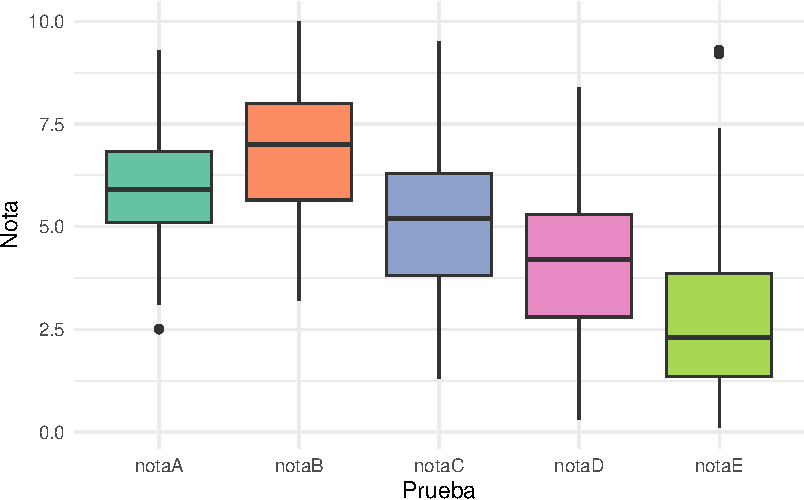
\includegraphics[keepaspectratio]{15-contrastes-medidas-repetidas_files/figure-pdf/boxplot-pruebas-1.pdf}}

}

\caption{Diagrama de cajas y bigotes de la nota en cada una de las cinco
pruebas.}

\end{figure}%

Como el interés de este capítulo está en las medidas repetidas sobre los
mismos individuos, conviene también visualizar la trayectoria de cada
alumno a través de las cinco pruebas. Para no saturar el gráfico se
representan solo los 10 primeros alumnos, junto con la trayectoria de la
media general (en rojo) calculada sobre todos los alumnos:

\begin{Shaded}
\begin{Highlighting}[]
\FunctionTok{ggplot}\NormalTok{(df\_largo }\SpecialCharTok{\%\textgreater{}\%} \FunctionTok{filter}\NormalTok{(alumno }\SpecialCharTok{\textless{}=} \DecValTok{10}\NormalTok{), }\FunctionTok{aes}\NormalTok{(}\AttributeTok{x =}\NormalTok{ prueba, }\AttributeTok{y =}\NormalTok{ nota)) }\SpecialCharTok{+}
  \FunctionTok{geom\_line}\NormalTok{(}\FunctionTok{aes}\NormalTok{(}\AttributeTok{group =}\NormalTok{ alumno), }\AttributeTok{alpha =} \FloatTok{0.4}\NormalTok{) }\SpecialCharTok{+}
  \FunctionTok{stat\_summary}\NormalTok{(}\AttributeTok{data =}\NormalTok{ df\_largo, }\FunctionTok{aes}\NormalTok{(}\AttributeTok{group =} \DecValTok{1}\NormalTok{), }\AttributeTok{fun =}\NormalTok{ mean, }\AttributeTok{geom =} \StringTok{"line"}\NormalTok{, }\AttributeTok{color =} \StringTok{"firebrick"}\NormalTok{, }\AttributeTok{linewidth =} \FloatTok{1.2}\NormalTok{) }\SpecialCharTok{+}
  \FunctionTok{labs}\NormalTok{(}\AttributeTok{x =} \StringTok{"Prueba"}\NormalTok{, }\AttributeTok{y =} \StringTok{"Nota"}\NormalTok{) }\SpecialCharTok{+}
  \FunctionTok{theme\_minimal}\NormalTok{()}
\end{Highlighting}
\end{Shaded}

\begin{figure}[H]

{\centering \pandocbounded{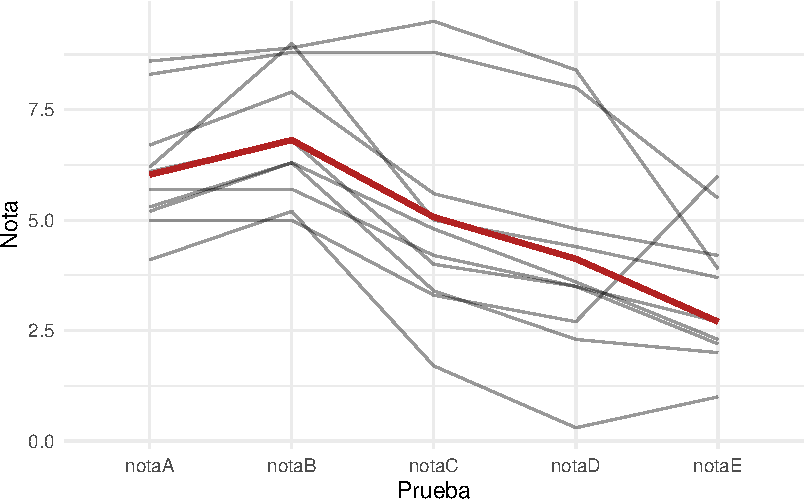
\includegraphics[keepaspectratio]{15-contrastes-medidas-repetidas_files/figure-pdf/lineas-trayectoria-1.pdf}}

}

\caption{Trayectoria de las notas de los 10 primeros alumnos a través de
las cinco pruebas, con la media general superpuesta en rojo.}

\end{figure}%

Tanto las cajas como las trayectorias individuales confirman la
tendencia descendente ya apuntada por las medias: la mayoría de los
alumnos obtiene notas cada vez más bajas a medida que avanzan las
pruebas, aunque con un orden entre alumnos que se mantiene
razonablemente estable (quien saca más nota en la prueba A tiende
también a sacar más nota en las siguientes).

\textbf{Comprobación de la normalidad}

El ANOVA de medidas repetidas que se presenta en la sección siguiente
exige que la variable sea normal en cada una de las medidas repetidas.
Antes de aplicarlo conviene comprobarlo, con el test de Shapiro-Wilk
visto en el capítulo de
\hyperref[contrastes-para-una-poblaciuxf3n]{contrastes para una
población}, en cada una de las cinco pruebas por separado:

\begin{Shaded}
\begin{Highlighting}[]
\NormalTok{df\_largo }\SpecialCharTok{\%\textgreater{}\%}
  \FunctionTok{group\_by}\NormalTok{(prueba) }\SpecialCharTok{\%\textgreater{}\%}
  \FunctionTok{summarise}\NormalTok{(}
    \AttributeTok{n =} \FunctionTok{sum}\NormalTok{(}\SpecialCharTok{!}\FunctionTok{is.na}\NormalTok{(nota)),}
    \StringTok{\textasciigrave{}}\AttributeTok{p{-}valor}\StringTok{\textasciigrave{}} \OtherTok{=} \FunctionTok{shapiro.test}\NormalTok{(nota[}\SpecialCharTok{!}\FunctionTok{is.na}\NormalTok{(nota)])}\SpecialCharTok{$}\NormalTok{p.value}
\NormalTok{  )}
\end{Highlighting}
\end{Shaded}

\begin{verbatim}
# A tibble: 5 x 3
  prueba     n  `p-valor`
  <fct>  <int>      <dbl>
1 notaA    120 0.907     
2 notaB    115 0.0675    
3 notaC    119 0.412     
4 notaD    118 0.575     
5 notaE    118 0.00000407
\end{verbatim}

En \texttt{notaA}, \texttt{notaB}, \texttt{notaC} y \texttt{notaD} el
p-valor del test de Shapiro-Wilk es superior a 0.05 (0.907, 0.068, 0.412
y 0.575, respectivamente), por lo que no hay evidencia para rechazar la
normalidad en ninguna de ellas. En \texttt{notaE}, en cambio, el p-valor
es \(4.07\times10^{-6}\), muy inferior a 0.05, por lo que se rechaza la
normalidad: esta última prueba tiene una distribución claramente no
normal (coherente con concentrar más alumnos suspensos en valores bajos,
lo que genera asimetría). El requisito de normalidad del ANOVA de
medidas repetidas no se cumple, por tanto, de forma estricta en las
cinco pruebas a la vez, lo que hace especialmente pertinente comprobar
también el resultado con la alternativa no paramétrica, el test de
Friedman, que se presenta a continuación.

\section{Comparación de las medidas
repetidas}\label{comparaciuxf3n-de-las-medidas-repetidas}

Con los datos ya en formato largo, el objetivo es contrastar si existen
diferencias entre las medias (o las distribuciones) de las cinco
pruebas. Según pueda asumirse o no la normalidad de las notas, se
dispone de una versión paramétrica (el ANOVA de medidas repetidas) y de
una alternativa no paramétrica (el test de Friedman).

\subsection{ANOVA de medidas repetidas de un
factor}\label{anova-de-medidas-repetidas-de-un-factor}

\begin{definition}[ANOVA de medidas repetidas de un
factor]\protect\hypertarget{def-medidasrepetidas-anova}{}\label{def-medidasrepetidas-anova}

El \emph{ANOVA de medidas repetidas de un factor} contrasta si las
medias de una variable cuantitativa son iguales en más de dos medidas
relacionadas (tomadas sobre los mismos individuos). La hipótesis nula es

\[H_0: \mu_1 = \mu_2 = \dots = \mu_k,\]

donde \(\mu_1, \dots, \mu_k\) son las medias poblacionales de las \(k\)
medidas repetidas, frente a la alternativa de que al menos una de esas
medias difiere de las demás.

\end{definition}

\textbf{Requisitos}: la variable dependiente debe ser cuantitativa y
seguir una distribución normal en cada una de las medidas repetidas (o
un tamaño muestral suficientemente grande en cada una). Además debe
cumplirse el supuesto de \textbf{esfericidad}, que exige que las
varianzas de las diferencias entre todos los pares posibles de medidas
repetidas sean aproximadamente iguales; cuando no se cumple, el
contraste se vuelve demasiado liberal (rechaza \(H_0\) con más facilidad
de la debida) y conviene corregirlo o recurrir a la alternativa no
paramétrica de la sección siguiente. Su comprobación formal (con el test
de esfericidad de Mauchly y correcciones como la de Greenhouse-Geisser)
queda fuera del alcance de este capítulo introductorio.

En R, el ANOVA de medidas repetidas se ajusta con la función
\texttt{aov()} habitual, pero añadiendo un término \texttt{Error()} que
identifica al alumno como la unidad sobre la que se repiten las medidas:
\texttt{Error(alumno/prueba)} indica que \texttt{prueba} varía dentro de
cada \texttt{alumno}. Este contraste exige que todos los individuos
tengan las cinco medidas completas, así que primero se eliminan de
\texttt{df\_largo} los alumnos con alguna nota perdida.

\begin{example}[]\protect\hypertarget{exm-medidasrepetidas-anova}{}\label{exm-medidasrepetidas-anova}

~

\begin{Shaded}
\begin{Highlighting}[]
\NormalTok{df\_largo\_completo }\OtherTok{\textless{}{-}}\NormalTok{ df\_largo }\SpecialCharTok{\%\textgreater{}\%}
  \FunctionTok{group\_by}\NormalTok{(alumno) }\SpecialCharTok{\%\textgreater{}\%}
  \FunctionTok{filter}\NormalTok{(}\SpecialCharTok{!}\FunctionTok{any}\NormalTok{(}\FunctionTok{is.na}\NormalTok{(nota))) }\SpecialCharTok{\%\textgreater{}\%}
  \FunctionTok{ungroup}\NormalTok{() }\SpecialCharTok{\%\textgreater{}\%}
  \FunctionTok{mutate}\NormalTok{(}\AttributeTok{alumno =} \FunctionTok{factor}\NormalTok{(alumno))}

\FunctionTok{n\_distinct}\NormalTok{(df\_largo\_completo}\SpecialCharTok{$}\NormalTok{alumno)}
\end{Highlighting}
\end{Shaded}

\begin{verbatim}
[1] 111
\end{verbatim}

\begin{Shaded}
\begin{Highlighting}[]
\NormalTok{modelo }\OtherTok{\textless{}{-}} \FunctionTok{aov}\NormalTok{(nota }\SpecialCharTok{\textasciitilde{}}\NormalTok{ prueba }\SpecialCharTok{+} \FunctionTok{Error}\NormalTok{(alumno}\SpecialCharTok{/}\NormalTok{prueba), }\AttributeTok{data =}\NormalTok{ df\_largo\_completo)}
\FunctionTok{summary}\NormalTok{(modelo)}
\end{Highlighting}
\end{Shaded}

\begin{verbatim}

Error: alumno
           Df Sum Sq Mean Sq F value Pr(>F)
Residuals 110  688.9   6.262               

Error: alumno:prueba
           Df Sum Sq Mean Sq F value Pr(>F)    
prueba      4 1122.2  280.56   192.5 <2e-16 ***
Residuals 440  641.4    1.46                   
---
Signif. codes:  0 '***' 0.001 '**' 0.01 '*' 0.05 '.' 0.1 ' ' 1
\end{verbatim}

De los 120 alumnos, 111 tienen las cinco notas completas y son los que
entran en el análisis (los 9 restantes se descartan por tener algún
valor perdido). El resultado se organiza en dos estratos: el primero
(\texttt{Error:\ alumno}) recoge la variabilidad debida a las
diferencias globales entre alumnos, y el segundo
(\texttt{Error:\ alumno:prueba}) es el que contiene el contraste de
interés, sobre \texttt{prueba}. El estadístico es \(F=192.5\) con 4 y
440 grados de libertad, y un p-valor inferior a \(2\times10^{-16}\), muy
por debajo de 0.05, por lo que se rechaza \(H_0\): existen diferencias
significativas entre las medias de las cinco pruebas. A la vista de las
medias descendentes ya observadas (de 6.03 en la prueba A a 2.70 en la
prueba E), la conclusión es que el nivel de exigencia (o el rendimiento
medio) no se mantiene constante a lo largo del curso.

\end{example}

El ANOVA de medidas repetidas solo informa de que \textbf{alguna} de las
cinco medias difiere de las demás, pero no de \textbf{cuáles}. Para
averiguarlo se puede completar el análisis con comparaciones por pares
(una versión del test t pareado para cada par de pruebas), corrigiendo
el nivel de significación de cada comparación individual con el método
de Bonferroni para controlar la probabilidad de cometer al menos un
error de tipo I al hacer varias comparaciones a la vez:

\begin{Shaded}
\begin{Highlighting}[]
\FunctionTok{pairwise.t.test}\NormalTok{(df\_largo\_completo}\SpecialCharTok{$}\NormalTok{nota, df\_largo\_completo}\SpecialCharTok{$}\NormalTok{prueba,}
                 \AttributeTok{paired =} \ConstantTok{TRUE}\NormalTok{, }\AttributeTok{p.adjust.method =} \StringTok{"bonferroni"}\NormalTok{)}
\end{Highlighting}
\end{Shaded}

\begin{verbatim}

    Pairwise comparisons using paired t tests 

data:  df_largo_completo$nota and df_largo_completo$prueba 

      notaA   notaB   notaC   notaD  
notaB < 2e-16 -       -       -      
notaC 2.1e-14 < 2e-16 -       -      
notaD < 2e-16 < 2e-16 < 2e-16 -      
notaE < 2e-16 < 2e-16 < 2e-16 7.9e-07

P value adjustment method: bonferroni 
\end{verbatim}

Los diez p-valores de la tabla son inferiores a 0.05 (el mayor, entre
\texttt{notaD} y \texttt{notaE}, es \(7.9\times10^{-7}\)), por lo que
las cinco pruebas difieren significativamente entre sí dos a dos: no se
trata de que una única prueba se aparte de las demás, sino de un
descenso generalizado y progresivo del rendimiento a lo largo de las
cinco pruebas.

\subsection{Test de Friedman}\label{test-de-friedman}

\begin{definition}[Test de
Friedman]\protect\hypertarget{def-medidasrepetidas-friedman}{}\label{def-medidasrepetidas-friedman}

El \emph{test de Friedman} es la alternativa no paramétrica al ANOVA de
medidas repetidas: contrasta si existen diferencias entre más de dos
medidas relacionadas sin necesidad de asumir que la variable sigue una
distribución normal. La hipótesis nula es

\[H_0: \mbox{no hay diferencias entre las medidas repetidas.}\]

El contraste se basa en los rangos que ocupa cada medida dentro de cada
individuo, en lugar de en los valores originales de la variable.

\end{definition}

\textbf{Requisitos}: la variable dependiente debe ser, al menos,
cualitativa ordinal (o cuantitativa), y las medidas deben proceder de
los mismos individuos. No exige normalidad, por lo que es la opción
adecuada cuando no puede garantizarse el requisito de normalidad (o de
esfericidad) del ANOVA de medidas repetidas.

En R, \texttt{friedman.test()} no trabaja sobre el formato largo, sino
que espera una matriz con los individuos en las filas y las medidas
repetidas en las columnas (es decir, prácticamente el formato ancho
original), y no admite valores perdidos, por lo que hay que eliminarlos
antes con \texttt{na.omit()}.

\begin{example}[]\protect\hypertarget{exm-medidasrepetidas-friedman}{}\label{exm-medidasrepetidas-friedman}

~

\begin{Shaded}
\begin{Highlighting}[]
\NormalTok{mat\_notas }\OtherTok{\textless{}{-}}\NormalTok{ df }\SpecialCharTok{\%\textgreater{}\%}
  \FunctionTok{select}\NormalTok{(notaA, notaB, notaC, notaD, notaE) }\SpecialCharTok{\%\textgreater{}\%}
  \FunctionTok{as.matrix}\NormalTok{() }\SpecialCharTok{\%\textgreater{}\%}
  \FunctionTok{na.omit}\NormalTok{()}

\FunctionTok{nrow}\NormalTok{(mat\_notas)}
\end{Highlighting}
\end{Shaded}

\begin{verbatim}
[1] 111
\end{verbatim}

\begin{Shaded}
\begin{Highlighting}[]
\FunctionTok{friedman.test}\NormalTok{(mat\_notas)}
\end{Highlighting}
\end{Shaded}

\begin{verbatim}

    Friedman rank sum test

data:  mat_notas
Friedman chi-squared = 316.59, df = 4, p-value < 2.2e-16
\end{verbatim}

Tras eliminar los valores perdidos quedan, de nuevo, 111 alumnos con las
cinco notas completas (los mismos que en el ANOVA anterior). El
estadístico del contraste es \(\chi^2=316.59\) con 4 grados de libertad
y un p-valor inferior a \(2.2\times10^{-16}\), muy inferior a 0.05, por
lo que también se rechaza \(H_0\): hay diferencias significativas entre
las cinco pruebas. La conclusión coincide plenamente con la del ANOVA de
medidas repetidas, lo cual es tranquilizador dado que, como se vio
antes, \texttt{notaE} no cumplía estrictamente el requisito de
normalidad: al no depender de ese supuesto, el resultado del test de
Friedman es, en este caso concreto, la referencia más fiable de las dos,
y el hecho de que ambos contrastes coincidan en su conclusión refuerza
la confianza en el resultado.

\end{example}

Al igual que con el ANOVA, el test de Friedman solo indica que existen
diferencias globales, no entre qué pares de pruebas concretas. La
versión no paramétrica de las comparaciones por pares, con la misma
corrección de Bonferroni, se obtiene con
\texttt{pairwise.wilcox.test()}:

\begin{Shaded}
\begin{Highlighting}[]
\FunctionTok{pairwise.wilcox.test}\NormalTok{(df\_largo\_completo}\SpecialCharTok{$}\NormalTok{nota, df\_largo\_completo}\SpecialCharTok{$}\NormalTok{prueba,}
                      \AttributeTok{paired =} \ConstantTok{TRUE}\NormalTok{, }\AttributeTok{p.adjust.method =} \StringTok{"bonferroni"}\NormalTok{)}
\end{Highlighting}
\end{Shaded}

\begin{verbatim}

    Pairwise comparisons using Wilcoxon signed rank test with continuity correction 

data:  df_largo_completo$nota and df_largo_completo$prueba 

      notaA   notaB   notaC   notaD  
notaB 1.3e-13 -       -       -      
notaC 8.8e-12 5.2e-16 -       -      
notaD < 2e-16 < 2e-16 < 2e-16 -      
notaE < 2e-16 < 2e-16 9.1e-13 8.8e-07

P value adjustment method: bonferroni 
\end{verbatim}

De nuevo los diez p-valores son inferiores a 0.05 (el mayor,
\(8.8\times10^{-7}\), vuelve a corresponder al par
\texttt{notaD}-\texttt{notaE}), confirmando con un método que no depende
de la normalidad la misma conclusión obtenida con las comparaciones
paramétricas: cada una de las cinco pruebas difiere significativamente
de las demás.

\begin{tcolorbox}[enhanced jigsaw, arc=.35mm, bottomrule=.15mm, bottomtitle=1mm, breakable, colback=white, colbacktitle=quarto-callout-tip-color!10!white, colframe=quarto-callout-tip-color-frame, coltitle=black, left=2mm, leftrule=.75mm, opacityback=0, opacitybacktitle=0.6, rightrule=.15mm, title=\textcolor{quarto-callout-tip-color}{\faLightbulb}\hspace{0.5em}{Tip}, titlerule=0mm, toprule=.15mm, toptitle=1mm]

Ante datos de medidas repetidas conviene aplicar primero el test de
Shapiro-Wilk (u otro contraste de normalidad) en cada una de las medidas
por separado. Si todas son razonablemente normales, el ANOVA de medidas
repetidas es la opción más potente; si alguna se aparta claramente de la
normalidad, como ocurre aquí con \texttt{notaE}, el test de Friedman es
la alternativa más segura. Cuando, como en este ejemplo, ambos
contrastes coinciden en su conclusión, puede reportarse cualquiera de
los dos con tranquilidad. La comprobación formal del supuesto adicional
de esfericidad que exige el ANOVA de medidas repetidas (con el test de
Mauchly y las correcciones de Greenhouse-Geisser o Huynh-Feldt) se
desarrolla con detalle en el
\href{https://aprendeconalf.es/estadistica-manual/}{Manual de
Estadística}.

\end{tcolorbox}

\section{Resumen}\label{resumen-1}

Los dos contrastes de este capítulo llegan a la misma conclusión: el
rendimiento de los alumnos no es constante a lo largo de las cinco
pruebas del curso, sino que desciende de forma significativa y, según
muestran las comparaciones por pares, de forma generalizada entre todas
ellas. Un resultado así, obtenido sobre datos de medidas repetidas,
sugiere una pregunta que el contraste estadístico por sí solo no puede
responder: si el descenso se debe a que las pruebas son cada vez más
difíciles, a que la materia se acumula y exige más al alumno conforme
avanza el curso, o a otra causa distinta (por ejemplo, cansancio o
pérdida de motivación); dar respuesta a esa pregunta exigiría un diseño
adicional, no solo un contraste de hipótesis.

Ambos contrastes son, además, la generalización, a más de dos medidas
repetidas, del contraste paramétrico visto en
\hyperref[contrastes-para-dos-poblaciones-pareadas]{Contrastes para dos
poblaciones pareadas} para el caso particular de solo dos medidas: de
hecho, cuando solo hay dos medidas repetidas, el estadístico F del ANOVA
de medidas repetidas coincide con el cuadrado del estadístico t del test
t pareado, y ambos contrastes dan exactamente el mismo p-valor. El test
de Friedman, en cambio, no se reduce al test de Wilcoxon para datos
pareados cuando solo hay dos medidas, porque Friedman se basa únicamente
en el orden (el rango) que ocupa cada medida dentro de cada individuo,
mientras que Wilcoxon tiene en cuenta también la magnitud de las
diferencias; con dos medidas, la generalización natural del test de
Friedman es más bien el test de los signos.

Con esto se cierra la parte de la tabla de decisión dedicada a comparar
medias o distribuciones entre dos o más poblaciones, ya sean
independientes o relacionadas; el
\href{16-relacion-entre-variables.qmd}{último capítulo de esta parte}
aborda una cuestión distinta: la relación y la predicción entre dos
variables cuantitativas.

\chapter{Relación y predicción entre dos
variables}\label{relaciuxf3n-y-predicciuxf3n-entre-dos-variables}

Este último capítulo cierra la tabla de decisión presentada en
\hyperref[selecciuxf3n-del-contraste-estaduxedstico-1]{Selección del
contraste estadístico} con las filas que faltaban: aquellas en las que
se quiere estudiar la \textbf{relación} entre dos variables
cuantitativas, o \textbf{predecir} una variable cuantitativa (o
cualitativa binaria) a partir de otra cuantitativa. La correlación y la
regresión son temas amplios, con mucha teoría, propiedades y variantes
detrás. Como ese desarrollo ya está hecho, y con detalle, en el
\href{https://aprendeconalf.es/estadistica-manual/}{Manual de
Estadística} del mismo autor, aquí no se repite: este capítulo se limita
a situar cada contraste en la tabla de decisión y a mostrar el ejemplo
mínimo de código en R necesario para aplicarlo sobre el conjunto de
datos del curso. Para las definiciones formales, las fórmulas y las
propiedades de estos contrastes, así como para el coeficiente
chi-cuadrado y el coeficiente de contingencia entre dos variables
cualitativas (mencionados pero no desarrollados en el capítulo
introductorio de esta parte), acúdase al Manual.

\section{Relación entre dos variables
cuantitativas}\label{relaciuxf3n-entre-dos-variables-cuantitativas}

Cuando ambas variables son cuantitativas y (aproximadamente) normales,
la pregunta habitual es si existe una \textbf{relación lineal} entre
ellas. El coeficiente de correlación de Pearson mide la fuerza y el
sentido de esa relación lineal, y toma valores en el intervalo
\([-1,1]\): cerca de \(1\) indica relación lineal positiva fuerte, cerca
de \(-1\) relación lineal negativa fuerte, y cerca de \(0\) ausencia de
relación lineal.

Cuando alguna de las variables es cualitativa ordinal, o cuando las
variables son cuantitativas pero no puede asumirse normalidad, se
utiliza en su lugar el coeficiente de correlación de Spearman, que mide
la relación de orden (monótona) entre las dos variables en lugar de la
relación estrictamente lineal. También toma valores en \([-1,1]\) y se
interpreta igual.

\begin{Shaded}
\begin{Highlighting}[]
\FunctionTok{cor.test}\NormalTok{(df}\SpecialCharTok{$}\NormalTok{notaA, df}\SpecialCharTok{$}\NormalTok{notaB, }\AttributeTok{method =} \StringTok{"pearson"}\NormalTok{)}
\end{Highlighting}
\end{Shaded}

\begin{verbatim}

    Pearson's product-moment correlation

data:  df$notaA and df$notaB
t = 14.709, df = 113, p-value < 2.2e-16
alternative hypothesis: true correlation is not equal to 0
95 percent confidence interval:
 0.7367182 0.8651991
sample estimates:
      cor 
0.8104926 
\end{verbatim}

El coeficiente de correlación de Pearson entre \texttt{notaA} y
\texttt{notaB} es \(r = 0.81\), y el contraste de hipótesis nula
\(H_0: \rho = 0\) da un p-valor prácticamente nulo
(\(p < 2.2 \times 10^{-16}\)), por lo que se rechaza la hipótesis nula:
existe una relación lineal positiva fuerte y significativa entre las dos
calificaciones.

\begin{Shaded}
\begin{Highlighting}[]
\FunctionTok{ggplot}\NormalTok{(df, }\FunctionTok{aes}\NormalTok{(}\AttributeTok{x =}\NormalTok{ notaB, }\AttributeTok{y =}\NormalTok{ notaA)) }\SpecialCharTok{+}
  \FunctionTok{geom\_point}\NormalTok{() }\SpecialCharTok{+}
  \FunctionTok{geom\_smooth}\NormalTok{(}\AttributeTok{method =} \StringTok{"lm"}\NormalTok{)}
\end{Highlighting}
\end{Shaded}

\begin{figure}[H]

{\centering \pandocbounded{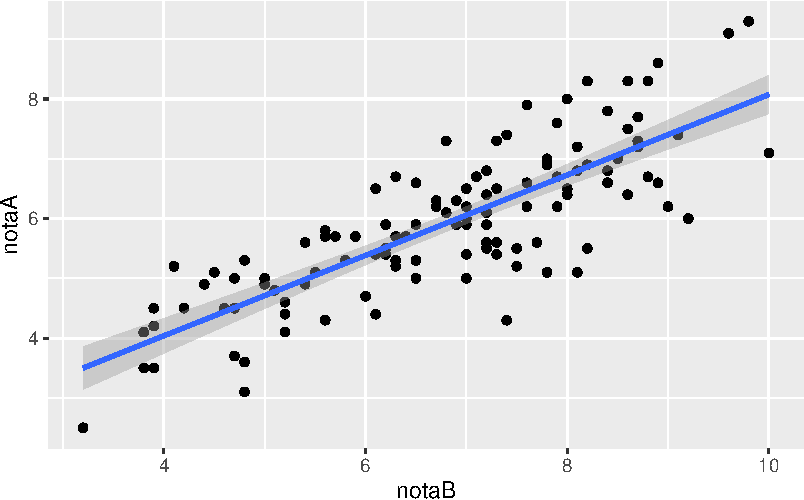
\includegraphics[keepaspectratio]{16-relacion-entre-variables_files/figure-pdf/unnamed-chunk-2-1.pdf}}

}

\caption{Diagrama de dispersión entre notaA y notaB, con la recta de
regresión ajustada.}

\end{figure}%

\section{Regresión simple}\label{regresiuxf3n-simple}

Cuando el objetivo no es solo contrastar si existe relación, sino
construir un \textbf{modelo predictivo} que permita estimar el valor de
una variable cuantitativa a partir de otra, se recurre a la regresión
lineal simple. El modelo ajusta la recta que mejor explica la variable
dependiente en función de la independiente, y el contraste de hipótesis
asociado a la pendiente indica si esa relación es estadísticamente
significativa.

\begin{Shaded}
\begin{Highlighting}[]
\NormalTok{modelo }\OtherTok{\textless{}{-}} \FunctionTok{lm}\NormalTok{(notaA }\SpecialCharTok{\textasciitilde{}}\NormalTok{ notaB, }\AttributeTok{data =}\NormalTok{ df)}
\FunctionTok{summary}\NormalTok{(modelo)}
\end{Highlighting}
\end{Shaded}

\begin{verbatim}

Call:
lm(formula = notaA ~ notaB, data = df)

Residuals:
     Min       1Q   Median       3Q      Max 
-2.02596 -0.46667  0.03761  0.46790  1.43947 

Coefficients:
            Estimate Std. Error t value Pr(>|t|)    
(Intercept)  1.34679    0.31938   4.217 5.02e-05 ***
notaB        0.67286    0.04575  14.709  < 2e-16 ***
---
Signif. codes:  0 '***' 0.001 '**' 0.01 '*' 0.05 '.' 0.1 ' ' 1

Residual standard error: 0.7501 on 113 degrees of freedom
  (5 observations deleted due to missingness)
Multiple R-squared:  0.6569,    Adjusted R-squared:  0.6539 
F-statistic: 216.3 on 1 and 113 DF,  p-value: < 2.2e-16
\end{verbatim}

Por cada punto que sube \texttt{notaB}, \texttt{notaA} sube en promedio
0.673 puntos (\(\hat\beta_1 = 0.673\)), y esa pendiente es
significativamente distinta de cero (\(p < 2\times10^{-16}\)), lo que
confirma la relación lineal ya detectada con la correlación. El
coeficiente de determinación, \(R^2 = 0.657\), indica que el modelo
explica un 65.7 \% de la variabilidad de \texttt{notaA}.

\section{Regresión logística
simple}\label{regresiuxf3n-loguxedstica-simple}

Cuando la variable que se quiere predecir es cualitativa binaria (por
ejemplo, aprobar o suspender una prueba) y la variable predictora es
cuantitativa, el modelo lineal deja de ser adecuado y se sustituye por
la regresión logística simple, que modela la probabilidad de la
categoría de interés en función de la variable independiente.

\begin{Shaded}
\begin{Highlighting}[]
\NormalTok{df }\OtherTok{\textless{}{-}}\NormalTok{ df }\SpecialCharTok{\%\textgreater{}\%}
  \FunctionTok{mutate}\NormalTok{(}\AttributeTok{aprobado =} \FunctionTok{as.numeric}\NormalTok{(calificacionA }\SpecialCharTok{==} \StringTok{"Aprobado"}\NormalTok{))}

\NormalTok{modelo\_log }\OtherTok{\textless{}{-}} \FunctionTok{glm}\NormalTok{(aprobado }\SpecialCharTok{\textasciitilde{}}\NormalTok{ notaE, }\AttributeTok{data =}\NormalTok{ df, }\AttributeTok{family =} \StringTok{"binomial"}\NormalTok{)}
\FunctionTok{summary}\NormalTok{(modelo\_log)}
\end{Highlighting}
\end{Shaded}

\begin{verbatim}

Call:
glm(formula = aprobado ~ notaE, family = "binomial", data = df)

Coefficients:
            Estimate Std. Error z value Pr(>|z|)   
(Intercept)  1.18250    0.40104   2.949  0.00319 **
notaE        0.03036    0.12613   0.241  0.80978   
---
Signif. codes:  0 '***' 0.001 '**' 0.01 '*' 0.05 '.' 0.1 ' ' 1

(Dispersion parameter for binomial family taken to be 1)

    Null deviance: 124.45  on 117  degrees of freedom
Residual deviance: 124.39  on 116  degrees of freedom
  (2 observations deleted due to missingness)
AIC: 128.39

Number of Fisher Scoring iterations: 4
\end{verbatim}

El coeficiente de \texttt{notaE} es positivo (\(\hat\beta_1 = 0.030\)),
lo que indicaría que una nota más alta en la prueba E se asocia a una
mayor probabilidad de aprobar la prueba A, pero el p-valor asociado
(\(p = 0.81\)) está muy lejos de ser significativo: con estos datos no
hay evidencia de que la calificación obtenida en la prueba E prediga el
resultado (aprobado/suspenso) de la prueba A.

\section{Cierre de esta parte del
libro}\label{cierre-de-esta-parte-del-libro}

Este libro ha recorrido dos preguntas distintas pero complementarias
sobre un mismo estudio estadístico. La primera parte trató sobre el
\textbf{diseño}: cómo se recogen los datos, según los distintos tipos de
estudios descriptivos, transversales, de cohortes, de casos y controles,
ecológicos, experimentales, cuasiexperimentales o basados en encuestas,
y qué conclusiones de causalidad permite extraer cada uno. La segunda
parte, cerrada con este capítulo, trató sobre el \textbf{análisis}: una
vez recogidos los datos, cómo elegir el contraste de hipótesis adecuado
según el número y el tipo de variables involucradas y la relación entre
las poblaciones comparadas. Conviene no perder de vista que ambas
preguntas son necesarias pero ninguna es suficiente por sí sola: un
contraste estadístico perfectamente elegido y ejecutado sobre datos mal
recogidos ---con sesgos de selección, factores de confusión no
controlados u otras amenazas a la validez discutidas en la primera
parte--- no produce conclusiones válidas, por muy pequeño que sea el
p-valor obtenido. El buen análisis estadístico empieza en el buen
diseño. Quien llegue a este capítulo sin haber pasado antes por el
principio del libro puede retomarlo en
\hyperref[introducciuxf3n-a-los-tipos-de-estudios-estaduxedsticos]{Introducción
a los tipos de estudios estadísticos}, y quien busque de nuevo el mapa
completo de contrastes puede volver a
\hyperref[selecciuxf3n-del-contraste-estaduxedstico-1]{Selección del
contraste estadístico}.




\end{document}
